\documentclass[12pt,a4paper]{report}

\usepackage{amsmath}
\usepackage{amssymb}
\usepackage{amsthm}
\usepackage{graphicx}
\usepackage{enumerate}
\usepackage[table]{xcolor}
\usepackage{verbatim}
\usepackage[top=1.2in, bottom=1.2in, left=1.2in, right=1.2in]{geometry}
%\usepackage[notref]{showkeys}

\usepackage{tikz}
\newcommand{\tikzmark}[2]{
	\tikz[overlay,remember picture, baseline] 
	\node[anchor=base] (#1) {$#2$};}

\usepackage{thmtools}
\renewcommand{\listtheoremname}{List of Applications}
\renewcommand\thmtformatoptarg[1]{: #1}

\usepackage{enotez}
\let\footnote=\endnote
\setenotez{list-name={Hints and Answers}, totoc=chapter}

\theoremstyle{definition}
\newtheorem{theorem}{Theorem}[chapter]
\newtheorem{lemma}[theorem]{Lemma}
\newtheorem{corollary}[theorem]{Corollary}
\newtheorem{definition}[theorem]{Definition}
\newtheorem{example}[theorem]{Example}
\newtheorem{properties}[theorem]{Properties}
\newtheorem{exercise}[theorem]{Exercise}
\newtheorem{exercise*}[theorem]{Exercise*}
\newtheorem{remark}[theorem]{Remark}
\newtheorem{sketch}[theorem]{Sketch}
\newtheorem*{application}{Application}

\newcommand{\figbox}[1]{
\begin{center}
	\fbox{\parbox[b][2.5in][t]{0.5\textwidth}{{\scriptsize{#1}}}}
\end{center}}
\newcommand*\rfrac[2]{{}^{#1}\!/_{#2}}
\newcommand{\wtd}[1]{\widetilde{#1}}
\newcommand{\abs}[1]{ \left| #1 \right| }
\newcommand{\rank}{\text{rank}\:}
\renewcommand{\d}{\mathrm{d}}
\newcommand{\e}{\mathrm{e}}
\newcommand{\df}[2]{\displaystyle{\frac{\partial #1}{\partial #2}}}
\newcommand{\ddf}[2]{\displaystyle{\frac{\partial^2 #1}{\partial #2^2}}}
\newcommand{\dff}[3]{\displaystyle{\frac{\partial^2 #1}{\partial{#2}\partial{#3}}}}
\newcommand{\Df}[2]{\displaystyle{\frac{\d #1}{\d #2}}}
\newcommand{\Ddf}[2]{\displaystyle{\frac{\d^2 #1}{\d #2^2}}}
\newcommand{\itgr}[4]{\int_{#1}^{#2} #3 \: \d #4}
\newcommand{\eval}[3]{\left. #1 \, \right|_{#2}^{#3}}

\setcounter{tocdepth}{2}

\title{A Compact Course on Mathematical Methods}
\author{Pascal Philipp}


\begin{document}

\maketitle

\newgeometry{top=1.0in, bottom=1.0in, left=0.7in, right=0.8in}
\noindent
\texttt{COMMENTS}
\thispagestyle{empty}
\newpage
\restoregeometry

\newgeometry{top=0.8in, bottom=1.0in, left=1.1in, right=1.1in}
\tableofcontents
\thispagestyle{empty}
\newpage
\listoftheorems[ignoreall,show={application}]

\bigskip
\noindent
\texttt{Customise the format: drop ``Application: ''.}
\thispagestyle{empty}
\restoregeometry

\addtocontents{toc}{\protect\thispagestyle{empty}}

\chapter{Vectors and Matrices}
\label{ch:vm}
\emph{Matrices} (singular: \emph{matrix}) are arrays of numbers, for example,
\[ M = \begin{bmatrix}
 4 & -\sqrt{3} & \pi \\ -5.2 & 0 & 13
\end{bmatrix}, \]
and \emph{vectors} are matrices that have only one column. The use of vectors and matrices makes the notation and handling of data and variables in large computations clearer and more compact, and their study has also led to new concepts and theories. Vectors and matrices are fundamental in mathematics and for applications of mathematical analysis.

In the example below, we will work with a matrix that represents the connections in a network of cities, and this matrix can therefore be considered the link that makes the road network accessible to mathematical analysis. Other networks that are frequently analysed using matrices include social networks (e.g., to study the spread of news), the world wide web (e.g., Google PageRank), contact networks (e.g., to minimise contagion in a hospital).

\begin{application}[Random walks]
A very large number of hikers is travelling randomly around the network of cities
\begin{center}
	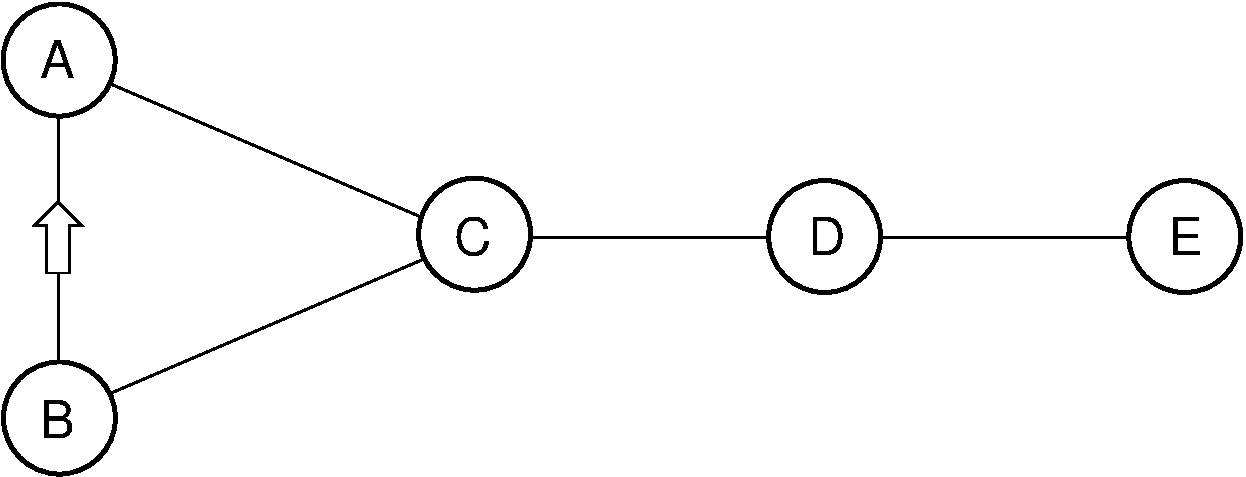
\includegraphics[width=0.5\textwidth]{./Figures/network.pdf}
\end{center}
where the road between $A$ and $B$ can only be travelled in one direction. A hiker would arrive in a city, stay for the day, randomly pick one of the outgoing roads -- each with equal probability; possibly the city he or she came from the previous day --  and then travel there the next morning. For example, if there are 100 hikers in $D$ today, then an average of 50 of them will hike to $C$ the next day. Besides those new arrivals from $D$, the city $C$ will further receive new hikers from $A$ and from $B$.

The hikers in this example are called \emph{random walkers} in mathematical jargon, and an important and applicable task is to find the \emph{steady state} of the system -- that is, the distribution of hikers so that the total number of hikers in each city does not change from one day to the next. For example, looking at the above map, you might expect that after a long time there should be a larger concentration of hikers in $C$ than in $E$.

The steady state  can be found by balancing the number of incoming and outgoing hikers for each city. Let $d$ and $e$ be the steady-state proportion of hikers in cities $D$ and $E$, and consider all travelling to and from $E$: outgoing $= e$, incoming = $\tfrac12d$, which gives $e = \tfrac12d$. Repeating this for the other cities leads to a collection of five equations.

Alternatively, one can choose a matrix approach and use vectors to describe the distribution of hikers over the network. The first entry of that vector stands for the proportion of hikers in $A$, the second for the proportion in $B$, etc. For example,
\[ v_1 = \begin{bmatrix} 0 \\ 0 \\ 1 \\ 0 \\ 0 \end{bmatrix}, \quad v_2 = \begin{bmatrix} 0.2 \\ 0.2 \\ 0.2 \\ 0.2 \\ 0.2 \end{bmatrix}\]
means in the first case that all hikers are in $C$, and in the second case that they are evenly distributed over all five cities. Next we describe their movements using a matrix. After the review of matrix multiplication in the next section, you will be able to convince yourself that
\[ v_{\text{tomorrow}} = \begin{bmatrix} 0 & \rfrac12 & \rfrac13 & 0 & 0 \\
									 0 & 0 & \rfrac13 & 0 & 0 \\
									 1 & \rfrac12 & 0 & \rfrac12 & 0 \\
									 0 & 0 & \rfrac13 & 0 & 1 \\
									 0 & 0 & 0 & \rfrac12 & 0 \end{bmatrix} v_{\text{today}}
					   = P \, v_{\text{today}} \]
reflects the movement of the hikers around the network of cities\footnote{For example:
\[ \text{all hikers in $C$} \leftrightarrow
v = \begin{bmatrix} 0 \\ 0 \\ 1 \\ 0 \\ 0 \end{bmatrix}
\quad \stackrel{P}{\longrightarrow} \quad
P \, v = \begin{bmatrix} \rfrac13 \\ \rfrac13 \\ 0 \\ \rfrac13 \\ 0 \end{bmatrix}
\leftrightarrow  \text{ hikers evenly distributed over $A,B,D$}
\qquad \text{\checkmark} \]
Now check this for the other four ``concentrated'' configurations. If that works, then $P$ is correct.
}. The task of finding a steady state now corresponds to finding a vector (i.e., a distribution of hikers) that does not change through application of $P$ (i.e., from one day to the next). Note that individual hikers keep moving -- the steady state is the distribution of hikers such that their \emph{total} number in each city stays the same. Denoting this vector by $v^*$ and its entries $a,b,c,d,e$, we obtain $v^*=Pv^*$, or
\[ \begin{bmatrix} a\\b\\c\\d\\e \end{bmatrix} =
\begin{bmatrix} 0 & \rfrac12 & \rfrac13 & 0 & 0 \\
0 & 0 & \rfrac13 & 0 & 0 \\
1 & \rfrac12 & 0 & \rfrac12 & 0 \\
0 & 0 & \rfrac13 & 0 & 1 \\
0 & 0 & 0 & \rfrac12 & 0 \end{bmatrix} \begin{bmatrix} a\\b\\c\\d\\e \end{bmatrix}. \]
This is an equation of 5-vectors (the result of the matrix multiplication on the right-hand side is a 5-vector as well) and therefore corresponds to a collection of five ordinary equations -- can you locate the equation $e = \tfrac12d$ from the previous paragraph in it?

The equation $v^*=Pv^*$ is in fact an eigenvalue equation for the matrix $P$. We will learn how to solve it in this chapter. The solution is
\[a=0.177,\:\:b=0.118,\:\:c=0.353,\:\:d=0.235,\:\:e=0.118\:.\]
\end{application}


\section{Review of Matrix Arithmetic}
\label{sec:rma}
\begin{definition}[Matrices] ~\\
\begin{enumerate}[(i)]
	\item A $m \times n$ matrix is an array
		\[A = \begin{bmatrix}
		a_{11} & a_{12} & a_{13} & \cdots & a_{1n} \\
		a_{21} & a_{22} & a_{23} & \cdots & a_{2n} \\
		a_{31} & a_{32} & a_{33} & \cdots & a_{3n} \\
		\vdots & \vdots & \vdots & \ddots & \vdots \\
		a_{m1} & a_{m2} & a_{m3} & \cdots & a_{mn} \\
		\end{bmatrix},\]
		where $m$ is the number of rows and $n$ the number of columns. We also refer to $A$ as a matrix of \emph{size} $m \times n$.
	\item An equation of the form $A=B$, where $A$ and $B$ are matrices of the same size $m \times n$, means that $a_{ij} = b_{ij}$ for all $i\in\{1,2,\dots,m\},j\in\{1,2,\dots,n\}.$ Matrices of different sizes can never be equal.
	\item Addition and subtraction can only be carried out for matrices of the same size, and then the operation is carried out elementwise:
		\begin{equation*}\begin{split}
		A \pm B & = \begin{bmatrix}
		a_{11} & a_{12} & \cdots & a_{1n} \\
		a_{21} & a_{22} & \cdots & a_{2n} \\
		\vdots & \vdots & \ddots & \vdots \\
		a_{m1} & a_{m2} & \cdots & a_{mn} \\
		\end{bmatrix} \pm \begin{bmatrix}
		b_{11} & b_{12} & \cdots & b_{1n} \\
		b_{21} & b_{22} & \cdots & b_{2n} \\
		\vdots & \vdots & \ddots & \vdots \\
		b_{m1} & b_{m2} & \cdots & b_{mn} \\
		\end{bmatrix} \\ & = \begin{bmatrix}
		a_{11} \pm b_{11} & a_{12} \pm b_{12} & \cdots & a_{1n} \pm b_{1n} \\
		a_{21} \pm b_{21} & a_{22} \pm b_{22} & \cdots & a_{2n} \pm b_{2n} \\
		\vdots & \vdots & \ddots & \vdots \\
		a_{m1} \pm b_{m1} & a_{m2} \pm b_{m2} & \cdots & a_{mn} \pm b_{mn} \\
		\end{bmatrix}.
		\end{split}\end{equation*}
	\item Multiplying a number with a matrix is called \emph{scalar multiplication}:
		\[ \lambda A = \lambda \begin{bmatrix}
		a_{11} & a_{12} & \cdots & a_{1n} \\
		a_{21} & a_{22} & \cdots & a_{2n} \\
		\vdots & \vdots & \ddots & \vdots \\
		a_{m1} & a_{m2} & \cdots & a_{mn} \\
		\end{bmatrix} = \begin{bmatrix}
		\lambda a_{11} & \lambda a_{12} & \cdots & \lambda a_{1n} \\
		\lambda a_{21} & \lambda a_{22} & \cdots & \lambda a_{2n} \\
		\vdots & \vdots & \ddots & \vdots \\
		\lambda a_{m1} & \lambda a_{m2} & \cdots & \lambda a_{mn} \\
		\end{bmatrix}.\]
	\item Multiplying two matrices $A$ and $B$ is called \emph{matrix multiplication} -- it can be carried out only if the number of columns of $A$ agrees with the number of rows of $B$:
		\begin{equation*}
		A \, B =\begin{bmatrix}
		a_{11} & a_{12} & \cdots & a_{1n} \\
		a_{21} & a_{22} & \cdots & a_{2n} \\
		\vdots & \vdots & \ddots & \vdots \\
		a_{m1} & a_{m2} & \cdots & a_{mn} \\
		\end{bmatrix} \begin{bmatrix}
		b_{11} & b_{12} & \cdots & b_{1k} \\
		b_{21} & b_{22} & \cdots & b_{2k} \\
		\vdots & \vdots & \ddots & \vdots \\
		b_{n1} & b_{n2} & \cdots & b_{nk} \\
		\end{bmatrix}
		= \begin{bmatrix}
		c_{11} & c_{12} & \cdots & c_{1k} \\
		c_{21} & c_{22} & \cdots & c_{2k} \\
		\vdots & \vdots & \ddots & \vdots \\
		c_{m1} & c_{m2} & \cdots & c_{mk} \\
		\end{bmatrix},
		\end{equation*}
		where $c_{ij} = \sum_{s=1}^n a_{is}b_{sj}$. The resulting matrix is of size $m \times k$.
	\item A \emph{square matrix} is a matrix with $m=n$. The \emph{identity matrix}, which has entries $1$ on the diagonal and is zero everywhere else,
	\[ I = \begin{bmatrix} 1 & & & \\ & 1 & & \\ & & \ddots & \\ & & & 1 \end{bmatrix},\]
	is an important example of a square matrix.
		
\end{enumerate}
\end{definition}

\begin{remark}
\begin{enumerate}[(i)]
	\item Regarding the condition on when two matrices can be multiplied, it should be useful to remember that ``$m \times n \cdot n \times k$ works and gives a $m \times k$ matrix.'' Therefore, the result of a $1 \times n$ with a $n \times 1$ is a $1 \times 1$, which is just a single real number, also called a \emph{scalar}.
	\item The rule for matrix multiplication may seem quite complicated -- it becomes easier to remember once one breaks down the procedure as follows. The case $1 \times n \cdot n \times 1$ just mentioned is the building block for matrix products:
\begin{equation*}\begin{split}
 \begin{bmatrix} a_{11} & a_{12} & a_{13} &\cdots & a_{1n} \end{bmatrix}
   \begin{bmatrix} b_{11} \\ b_{21} \\ b_{31} \\ \vdots \\ b_{n1} \end{bmatrix}
   & = a_{11}b_{11} + a_{12}b_{21} + a_{13}b_{31} + \dots + a_{1n}b_{n1} \\
   & = \sum_{s=1}^n a_{1s}b_{s1} = c_{11} \:.
\end{split}\end{equation*}
Here, both matrices have the same number of elements, and those entries are multiplied pairwise and then added up. For larger matrices, one just repeats this procedure $m \cdot k$ times:
\[\left[ \begin{array}{cccc}
\rowcolor{olive!20}
a_{11} & a_{12} & \cdots & a_{1n} \\
a_{21} & a_{22} & \cdots & a_{2n} \\
\vdots & \vdots & \ddots & \vdots \\
a_{m1} & a_{m2} & \cdots & a_{mn} \\
\end{array} \right] \left[ \begin{array}{c>{\columncolor{olive!20}}ccc}
b_{11} & b_{12} & \cdots & b_{1k} \\
b_{21} & b_{22} & \cdots & b_{2k} \\
\vdots & \vdots & \ddots & \vdots \\
b_{n1} & b_{n2} & \cdots & b_{nk} \\
\end{array} \right]
= \left[ \begin{array}{cccc}
c_{11} & \cellcolor{olive!20} c_{12} & \cdots & c_{1k} \\
c_{21} & c_{22} & \cdots & c_{2k} \\
\vdots & \vdots & \ddots & \vdots \\
c_{m1} & c_{m2} & \cdots & c_{mk} \\
\end{array} \right]. \]
	\item Another important definition for matrices is the \emph{transpose} of a matrix, which leaves the entries $a_{11}, a_{22}, a_{33}, \dots$ alone and swaps all other entries across the diagonal. This operation is denoted with a ``$^\top$'' and changes the size of the matrix unless it is square, cf. the examples below.
\end{enumerate}	
\end{remark}

\begin{example}
\begin{enumerate}[(i)]
	\item The $2 \times 2$ identity matrix is $I = \begin{bmatrix} 1 & 0 \\ 0 & 1 \end{bmatrix}.$
	\item The matrix
	\[ A = \begin{bmatrix}
	1 & 2 \\ 3 & 4 \\ 5 & 6
	\end{bmatrix}\]
	is of size $3 \times 2$ and its transpose is the $2 \times 3$ matrix
	\[ A^{\top} = \begin{bmatrix}
	1 & 3 & 5 \\ 2 & 4 & 6
	\end{bmatrix}.\]
	\item For the matrix $A$ from (ii), we have
	\[ A + A = \begin{bmatrix}
	1 & 2 \\ 3 & 4 \\ 5 & 6
	\end{bmatrix} + \begin{bmatrix}
	1 & 2 \\ 3 & 4 \\ 5 & 6
	\end{bmatrix} = \begin{bmatrix}
	1+1 & 2+2 \\ 3+3 & 4+4 \\ 5+5 & 6+6
	\end{bmatrix} = \begin{bmatrix}
	2 & 4 \\ 6 & 8 \\ 10 & 12
	\end{bmatrix},\]
	which agrees with
	\[ 2 \, A = 2 \, \begin{bmatrix}
	1 & 2 \\ 3 & 4 \\ 5 & 6
	\end{bmatrix} = \begin{bmatrix}
	2\cdot1 & 2\cdot2 \\ 2\cdot3 & 2\cdot4 \\ 2\cdot5 & 2\cdot6
	\end{bmatrix} = \begin{bmatrix}
	2 & 4 \\ 6 & 8 \\ 10 & 12
	\end{bmatrix}.\]
	\item For $A$ and its transpose $A^\top$, we obtain the products
	\begin{equation*} \begin{split}
	A \, A^\top & = \begin{bmatrix}
	1 & 2 \\ 3 & 4 \\ 5 & 6
	\end{bmatrix} \begin{bmatrix}
	1 & 3 & 5 \\ 2 & 4 & 6
	\end{bmatrix} \\ & = \begin{bmatrix}
	 1 \cdot 1 + 2 \cdot 2 & 1 \cdot 3 + 2 \cdot 4 & 1 \cdot 5 + 2 \cdot 6 \\
	 3 \cdot 1 + 4 \cdot 2 & 3 \cdot 3 + 4 \cdot 4 & 3 \cdot 5 + 4 \cdot 6 \\ 
	 5 \cdot 1 + 6 \cdot 2 & 5 \cdot 3 + 6 \cdot 4 & 5 \cdot 5 + 6 \cdot 6
	\end{bmatrix} = \begin{bmatrix}
	5 & 11 & 17 \\ 11 & 25 & 39 \\ 17 & 39 & 61
	\end{bmatrix}
	\end{split} \end{equation*}
	and
	\begin{equation*}\begin{split}
    A^\top A & = \begin{bmatrix}
	1 & 3 & 5 \\ 2 & 4 & 6
	\end{bmatrix} \begin{bmatrix}
	1 & 2 \\ 3 & 4 \\ 5 & 6
	\end{bmatrix} \\ & = \begin{bmatrix}
	1 \cdot 1 + 3 \cdot 3 + 5 \cdot 5 & 1 \cdot 2 + 3 \cdot 4 + 5 \cdot 6 \\
	2 \cdot 1 + 4 \cdot 3 + 6 \cdot 5 & 2 \cdot 2 + 4 \cdot 4 + 6 \cdot 6
	\end{bmatrix} = \begin{bmatrix}
	35 & 44 \\ 44 & 56
	\end{bmatrix}.
	\end{split}\end{equation*}
\end{enumerate}
\end{example}

\begin{properties}
	\label{prop:matrix_mult}
	\begin{enumerate}[(i)]
		\item Matrix addition is commutative and associative:
		\[ A + B = B + A \:, \qquad A+B+C = (A+B)+C = A+(B+C) \:, \]
		where all three matrices are of the same size.
		\item Matrix multiplication is associative as well, but it is not commutative. That is, $AB$ is not always the same as $BA$. However, scalars can be swapped with matrices,
		\[ A(\lambda B) = \lambda A B \:. \]
		\item For combinations of the two operations, distributive laws hold:
		\[ A (B+ \wtd{B}) = AB + A\wtd{B} \:, \qquad (A+\wtd{A})B = AB + \wtd{A}B \:,\]
		where $A,\wtd{A}$ are $m \times n$ and $B,\wtd{B}$ are $n \times k$.
		\item For the transpose of a matrix multiplication, we have
		\[ (AB)^\top = B^\top A^\top,\]
		where the sizes of $A$ and $B$ are as in the previous property.
	\end{enumerate}
\end{properties}

\begin{definition}[Vectors]
\label{def:vectors}
~\\
\begin{enumerate}[(i)]
	\item A $n$-vector is a $n \times 1$ matrix:
		\[v = \begin{bmatrix}
		v_1 \\
		v_2 \\
		v_3 \\
		\vdots \\
		v_n \\
		\end{bmatrix}.\]
		We also refer to $v$ as a vector of size $n$.
	\item As for matrices, $v=w$ means that $v_i = w_i$ for all $i\in\{1,2,\dots,n\}$, and vectors of different sizes can never be equal. In equations like 
	\[ v = 0 \:, \]
	the $0$ on the right-hand side is understood to stand for the $n \times 1$ vector of all zeros rather than the number zero. 
	\item Addition and subtraction can only be carried out for vectors of the same size, and then the operation is carried out elementwise:
		\begin{equation*}
		v \pm w = \begin{bmatrix}
		v_1 \\
		v_2 \\
		\vdots \\
		v_n \\
		\end{bmatrix} \pm \begin{bmatrix}
		w_1 \\
		w_2 \\
		\vdots \\
		w_n \\
		\end{bmatrix} \\ = \begin{bmatrix}
		v_1 \pm w_1 \\
		v_2 \pm w_2 \\
		\vdots \\
		v_n \pm w_n \\
		\end{bmatrix}.
		\end{equation*}
	\item Multiplying a number with a vector is called scalar multiplication:
		\[ \lambda v = \lambda \begin{bmatrix}
		v_1 \\
		v_2 \\
		\vdots \\
		v_n \\
		\end{bmatrix} = \begin{bmatrix}
		\lambda v_1 \\
		\lambda v_2 \\
		\vdots \\
		\lambda v_n \\
		\end{bmatrix}. \]
	\item Multiplication of a matrix and a vector is carried out according to the rules of matrix multiplication: If the number of columns of $A$ agrees with the size of $v$, then
		\begin{equation*}
		A \, v =\begin{bmatrix}
		a_{11} & a_{12} & \cdots & a_{1n} \\
		a_{21} & a_{22} & \cdots & a_{2n} \\
		\vdots & \vdots & \ddots & \vdots \\
		a_{m1} & a_{m2} & \cdots & a_{mn} \\
		\end{bmatrix} \begin{bmatrix}
		v_1 \\
		v_2 \\
		\vdots \\
		v_n \\
		\end{bmatrix}
		= \begin{bmatrix}
		c_1 \\
		c_2 \\
		\vdots \\
		c_m \\
		\end{bmatrix},
		\end{equation*}
		where $c_i = \sum_{s=1}^n a_{is}v_{s}$. The result is a vector of size $m$.
	\item The \emph{scalar product} (or \emph{dot product}) of two vectors $v$ and $w$ of the same size is
		\[ v \circ w = \begin{bmatrix} v_1 \\ v_2 \\ \vdots \\ v_n \end{bmatrix} \circ
					   \begin{bmatrix} w_1 \\ w_2 \\ \vdots \\ w_n \end{bmatrix}
					   = \sum_{s=1}^n v_s w_s \:. \]
	\item A \emph{row vector} of size $n$ is a $1 \times n$ matrix:
	\[v = \begin{bmatrix}
	v_1 & v_2 & v_3 & \cdots & v_n \end{bmatrix}. \]
	\item The \emph{norm} of a vector is
	\[ ||v|| = \sqrt{v_1^2+v_2^2+ \dots v_n^2} = \sqrt{v \circ v} \:. \]
	\end{enumerate}
\end{definition}

\begin{remark}
\label{rem:vectors}
\begin{enumerate}[(i)]
	\item The term ``vector'' always refers to a one-column matrix as in (i) of Definition~\ref{def:vectors}, and it is sometimes called \emph{column vector} to distinguish it more explicitly from a row vector. Note that parts (i)-(v) of~\ref{def:vectors} are inherited from the corresponding matrix definitions, and only (vi)-(viii) are new and specific to vectors. Regarding multiplication and products: a simple dot ``$\cdot$'' stands either for regular multiplication of two numbers, for scalar multiplication (multiplication of a number with a vector or matrix), or for matrix multiplication (multiplication of matrices and vectors of appropriate size). However, the ``$\cdot$'' may be omitted. For scalar products, we always write the~``$\circ$''.
	\item The matrix transpose allows to write the scalar product of two vectors as a matrix product: Let $v,w$ be two vectors of the same size, then
	\[ v \circ w = v^\top w \:. \]
	\item When defining a vector in-line, it is more convenient to write down its transpose. For example, $v = \begin{bmatrix} 2 & -1 & 3 \end{bmatrix}^\top$ is the vector
	\[ v = \begin{bmatrix} 2 \\ -1 \\ 3 \end{bmatrix}. \]
	\item We write $v\in\mathbb{R}^n$ for a vector of size $n$, meaning that $v$ has $n$ entries and each of them is a real number. For $n=2$ or $n=3$~: Picturing a vector as an arrow in the two-dimensional plane $\mathbb{R}^2$ or in the three-dimensional space $\mathbb{R}^3$, the norm $||v||$ is simply its length. The angle $\theta$ between two vectors $v$ and $w$ of the same size is
	\[ \cos \theta = \frac{v \circ w}{||v|| \, ||w||} \:. \]
	\end{enumerate}
\end{remark}

\begin{example}
\begin{enumerate}[(i)]
	\item \[ \begin{bmatrix}
	11 \\ -6 \\ 6
	\end{bmatrix} - \begin{bmatrix}
	-7 \\ -1 \\ 3
	\end{bmatrix} = \begin{bmatrix}
	18 \\ -5 \\ 3
	\end{bmatrix} \]
	\item \[ \begin{bmatrix}
	4 & -1 \\ 0 & -3 \\ 7 & 1
	\end{bmatrix} \begin{bmatrix}
	-9 \\ 3
	\end{bmatrix} = \begin{bmatrix}
	4 \cdot (-9) + (-1) \cdot 3 \\
	0 \cdot (-9) + (-3) \cdot 3 \\
	7 \cdot (-9) + 1 \cdot 3 \\
	\end{bmatrix} = \begin{bmatrix}
	-39 \\ -9 \\ -60
	\end{bmatrix}\]
	\item The scalar product of $v = \begin{bmatrix} 4 & - 4 & 1 \end{bmatrix}^\top$
	and $w = \begin{bmatrix} 3 & -2 & -5\end{bmatrix}^\top$ is
	\[ v \circ w = \begin{bmatrix} 4 \\ -4 \\ 1 \end{bmatrix} \circ
	\begin{bmatrix} 3 \\ -2 \\ -5\end{bmatrix} 
	= 4 \cdot 3 + (-4) \cdot (-2) + 1 \cdot (-5) = 15 \:. \]
	\item The scalar product in the previous example can also be computed as a matrix multiplication, namely $v^\top w =15$. Transposing the second vector instead gives a $3 \times 3$ matrix:
	\begin{equation*}
	\begin{split}
v w^\top &= \begin{bmatrix} 4 \\ -4 \\ 1 \end{bmatrix} 
\begin{bmatrix} 3 & -2 & -5\end{bmatrix} \\ &= \begin{bmatrix}
4 \cdot 3 & 4 \cdot (-2) & 4 \cdot (-5) \\
(-4) \cdot 3 & (-4) \cdot (-2) & (-4) \cdot (-5) \\
1 \cdot 3 & 1 \cdot (-2) & 1 \cdot (-5) \\
\end{bmatrix} = \begin{bmatrix}
12 & -8 & -20 \\ -12 & 8 & 20 \\ 3 & -2 & -5 
\end{bmatrix}.
	\end{split}
	\end{equation*}
	\item 
	\[ \begin{bmatrix}
	0 & -2 & 13
	\end{bmatrix} \begin{bmatrix}
	3 & 2 & -4 \\ 5 & -3 & 0 \\ 1 & -2 & 1
	\end{bmatrix} \begin{bmatrix}
	3 \\ 7 \\ -1
	\end{bmatrix} = \begin{bmatrix}
	0 & -2 & 13	
	\end{bmatrix} \begin{bmatrix}
	27 \\ -6 \\ -12
	\end{bmatrix} = -144 \]
	\item The norm of $v=\begin{bmatrix}1 & 2 & 3\end{bmatrix}^\top$ is
	\[ ||v|| = \sqrt{1^2+2^2+3^2} = \sqrt{14} \:. \]
	For its angle with $\begin{bmatrix}3 & 2 & 1\end{bmatrix}^\top$, we find
	\[ \cos \theta = \frac{3+4+3}{\sqrt{14}\sqrt{14}} = \frac57 \:, \]
	which gives $\theta = \arccos \left(\rfrac57\right) \approx 0.7752$ (this angle is in radians and corresponds to $44.42$ degrees; here, $\arccos$ is the inverse function of $\cos$).
\end{enumerate}
\end{example}

\begin{definition}[Determinants]
The \emph{determinant} of a square matrix is a scalar and defined as follows for matries of sizes up to $3 \times 3$.
\begin{enumerate}[(i)]
	\item The determinant of a $1 \times 1$ matrix is
	\[ \det \begin{bmatrix} a_{11} \end{bmatrix} = a_{11} \:. \]
	\item The determinant of a $2 \times 2$ matrix is
	\[ \det\begin{bmatrix} a_{11} & a_{12} \\ a_{21} & a_{22} \end{bmatrix}
	= a_{11}a_{22} - a_{21}a_{12} \:. \]
	\item The determinant of a $3 \times 3$ matrix is
	\begin{equation*}
	\begin{split} \det\begin{bmatrix} a_{11} & a_{12} & a_{13} \\ a_{21} & a_{22} & a_{23} \\ a_{31} & a_{32} & a_{33} \end{bmatrix} = a_{11}a_{22}a_{33} + & a_{12}a_{23}a_{31} + a_{13}a_{21}a_{32} \\ & - a_{31}a_{22}a_{13} - a_{32}a_{23}a_{11} - a_{33}a_{21}a_{12} \:.
	\end{split}
	\end{equation*}
\end{enumerate}
\end{definition}

\begin{remark}
\begin{enumerate}[(i)]
	\item One can write $\abs{\dots}$ as an abbreviation for $\det\begin{bmatrix} \dots \end{bmatrix}$.
	\item Determinants of $1 \times 1$ matrices are quite straightforward; for $2 \times 2$, subtract the product of the off-diagonal entries from the product of the diagonal entries; see the following two points for $3 \times 3$. Determinants are also defined for larger square matrices, but the formulas become quite bulky then and one would not write them out as in the definition above.
	\item Sarrus' rule should help you memorise the formula for the determinant of a $3 \times 3$ matrix: For $A$ with entries as in (iii) of the definition above, write down $A$, copy the first two columns and append them to the right of the matrix; draw (or imagine) the lines
	\[ \begin{array}{ccccc}
		\tikzmark{A11}{a_{11}} & \tikzmark{A12}{a_{12}} & \tikzmark{A13}{a_{13}} & \tikzmark{A11A}{a_{11}} & \tikzmark{A12A}{a_{12}} \\
		a_{21} & a_{22} & a_{23} & a_{21} & a_{22} \\
		\tikzmark{A31}{a_{31}} & \tikzmark{A32}{a_{32}} & \tikzmark{A33}{a_{33}} & \tikzmark{A31A}{a_{31}} & \tikzmark{A32A}{a_{32}} \\
	\end{array} \:; \]
	\begin{tikzpicture}[overlay,remember picture]
%	\draw (A11.center) -- (A33.center);
%	\draw (A12.center) -- (A31A.center);
%	\draw (A13.center) -- (A32A.center);
%	\draw[dashed] (A31.center) -- (A13.center);
%	\draw[dashed] (A32.center) -- (A11A.center);
%	\draw[dashed] (A33.center) -- (A12A.center);
	\draw[opacity=.3,line width=4mm,line cap=round,draw=blue] (A11.center) -- (A33.center);
	\draw[opacity=.3,line width=4mm,line cap=round,draw=blue] (A12.center) -- (A31A.center);
	\draw[opacity=.3,line width=4mm,line cap=round,draw=blue] (A13.center) -- (A32A.center);
	\draw[opacity=.3,line width=4mm,line cap=round,draw=red] (A31.center) -- (A13.center);
	\draw[opacity=.3,line width=4mm,line cap=round,draw=red] (A32.center) -- (A11A.center);
	\draw[opacity=.3,line width=4mm,line cap=round,draw=red] (A33.center) -- (A12A.center);
	\end{tikzpicture}
	
	add up the products of the entries in each blue line, and subtract the three red products.
	\item Laplace's formula:
	\[ \begin{vmatrix}
	a_{11} & a_{12} & a_{13} \\ a_{21} & a_{22} & a_{23} \\ a_{31} & a_{32} & a_{33}
	\end{vmatrix} = a_{11}\begin{vmatrix}
	a_{22} & a_{23} \\ a_{32} & a_{33}
	\end{vmatrix} - a_{12}\begin{vmatrix}
	a_{21} & a_{23} \\ a_{31} & a_{33}	
	\end{vmatrix} + a_{13}\begin{vmatrix}
	a_{21} & a_{22} \\ a_{31} & a_{32}
	\end{vmatrix} \:. \]
	Here we have ``developed'' the determinant along the first row $(a_{11},a_{12},a_{13})$, but it is also possible to develop along a different row or even along a column. The general formulas are
	\begin{equation}
	\label{eq:laplace}
	\begin{split}
	\det A & = \sum_{j=1}^3 (-1)^{i+j} a_{ij} \det \wtd{A}_{ij}
	\qquad \text{(dev. along $i$-th row),} \\
	\det A & = \sum_{i=1}^3 (-1)^{i+j} a_{ij} \det \wtd{A}_{ij} \qquad \text{(dev. along $j$-th column),}
	\end{split}
	\end{equation}
	where $\wtd{A}_{ij}$ is the $2 \times 2$ matrix we obtain by removing the $i$-th row and the $j$-th column from $A$. Choose the row/column wisely! For example, if there is a row or a column with only one nonzero entry, developing along it will shorten the computation.
	\item Laplace's formula generalises to larger square matrices -- just replace the maximum index $3$ of the sums in~\eqref{eq:laplace} with $n$. Note that Laplace's formula does not directly compute determinants -- it reduces the problem of finding a $n \times n$ determinant to finding the determinants of $n$ matrices of size $(n-1) \times (n-1)$. Sarrus' rule works only for $3 \times 3$'s, it can not be applied to larger matrices.
\end{enumerate}
\end{remark}

\begin{example}
\begin{enumerate}[(i)]
		\item \[ \begin{vmatrix} 1 & 2 \\ 3 & 4 \end{vmatrix} = 1 \cdot 4 - 2 \cdot 3 = -2 \]
		\item \[ \begin{vmatrix} 1 & 2 & 3 \\ 4 & 5 & 6 \\ 7 & 8 & 9 \end{vmatrix} = 1 \cdot 5 \cdot 9 + 2 \cdot 6 \cdot 7 + 3 \cdot 4 \cdot 8 - 7 \cdot 5 \cdot 3 - 8 \cdot 6 \cdot 1 - 9 \cdot 4 \cdot 2 = 0 \]
		\item \[ \begin{vmatrix} 1 & -3 & 2 \\ 0 & 7 & -1 \\ 0 & 0 & -3 \end{vmatrix} = 1 \cdot 7 \cdot (-3) = -21 \]
		\item To compute the determinant of 
\[ A = \begin{bmatrix} 4 & -1 & 11 & 3  \\ -2 & 3 & -3 & -5 \\ 
0 & 1 & -8 & 0 \\ 1 & 0 & -6 & -2 \end{bmatrix}, \]
we use Laplace's formula, developing along the row with the most zero entries:
\begin{equation*}
\begin{split}
\det A 
& = (-1)^{3+1} \cdot 0 \begin{vmatrix} \ldots \end{vmatrix}
+ (-1)^{3+2} \cdot 1 \begin{vmatrix} \ldots \end{vmatrix}
+ (-1)^{3+3} \cdot (-8) \begin{vmatrix} \ldots \end{vmatrix} \\
& \quad + (-1)^{3+4} \cdot 0 \begin{vmatrix} \ldots \end{vmatrix} 
= - \begin{vmatrix} 4 & 11 & 3 \\ -2 & -3 & -5 \\ 1 & -6 & -2 \end{vmatrix}
- 8 \begin{vmatrix} 4 & -1 & 3 \\ -2 & 3 & -5 \\ 1 & 0 & -2 \end{vmatrix} \\ 
& = -4\begin{vmatrix} -3 & -5 \\ -6 & -2 \end{vmatrix} 
+11\begin{vmatrix} -2 & -5 \\ 1 & -2 \end{vmatrix}
-3\begin{vmatrix} -2 & -3 \\ 1 & -6 \end{vmatrix}
-8\cdot\begin{vmatrix} \ldots \end{vmatrix} = \ldots = 342 \:.  
\end{split}
\end{equation*}
\end{enumerate}
\end{example}

\begin{properties}
	\label{prop:det}
	Let $A$ be a $n \times n$ matrix and let $\lambda$ be a scalar.
	\begin{enumerate}[(i)]
		\item If $A$ has a row or a column of zeros, then $\det A=0$.
		\item If a row of $A$ is a multiple of some other row of $A$, then $\det A =0$. Similar for columns.
		\item If $A$ is an upper triangular matrix,
		\[ A = \begin{bmatrix} 
		a_{11} & a_{12} & a_{13} & \cdots & a_{1n}\\
		0      & a_{22} & a_{23} &        & a_{2n}\\
		0      & 0      & a_{33} &        & a_{3n}\\
		\vdots &        & \ddots & \ddots &\vdots \\
		0      & 0      & \cdots & 0 & a_{nn} 
		\end{bmatrix}, \]
		then the determinant is just the product along the diagonal, 
		\[ \det A = a_{11} a_{22} a_{33} \dots a_{nn} \:. \]
	\end{enumerate}
\end{properties}

\begin{application}[Orthogonal projection]
	A data scientist is working on a large data set of the form
	\[\{(x_1,y_1), (x_2,y_2), (x_3,y_3), \dots, (x_n,y_n)\} \:. \]
	She begins her analysis by plotting all data points in the $xy$-plane:
	%\figbox{Data in the $xy$-plane:}
	\begin{center}
		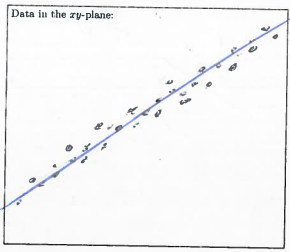
\includegraphics[width=0.6\textwidth]{./Figures/f201.png}
	\end{center}
	Here, $n$ individuals or events were observed, and two pieces of information were recorded for each individual/event (e.g., $n$ patients, $x_k$ stands for the score on a certain medical test, and $y_k$ stands for the score on a different test). Note that the data points are concentrated around a line. The data scientist has computed the slope of the line -- we will learn how fit lines through data later -- and now wants to project the data points onto it. One of the main advantages of this step is that the projected data will then be one-dimensional. That is, each point can then be described by one real number, namely its position along the line. This reduction can make a significant difference for the overall computational complexity of big data projects.
	
	We now derive how to project points \emph{orthogonally} onto a line. Let $L\subseteq\mathbb{R}^2$ be a line and let $w\in\mathbb{R}^2$ be a point that is not an element of $L$. Denote the projection of $w$ onto $L$ by $\wtd{w}$. To project orthogonally means that the line segment connecting $w$ and $\wtd{w}$ is orthogonal to $L$. Let $v$ be a vector that spans $L$, i.e. $L$ is the set of all scalar multiples of $V$,
	\[ L = \{ \lambda v \: | \: \lambda \in \mathbb{R} \} \subseteq \mathbb{R}^2 \:. \]
	This looks as follows, and the goal is now to find a formula for $\wtd{w}$ in terms of $v$ and~$w$.
	%\figbox{Orth. proj. onto a line:}
	\begin{center}
		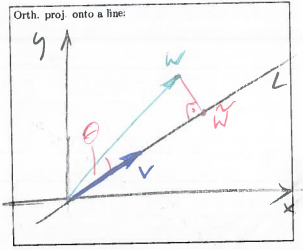
\includegraphics[width=0.6\textwidth]{./Figures/f202.png}
	\end{center}
	
	To visualise elements of $\mathbb{R}^2$, we are using two interpretations interchangeably: $w$ can be interpreted as a point, e.g.,
	\[ w = (1,2) \:, \]
	or as a vector,
	\[ w = \begin{bmatrix} 1 \\ 2 \end{bmatrix}, \]
	where the latter is often drawn as an arrow. Basing the arrow at the origin $(0,0)$ of the $xy$-plane, and interpreting it as ``move $1$ in the $x$ direction and $2$ in the $y$ direction'', we see that the vector $w$ points to the point $w$. This correspondence justifies switching freely between the two interpretations.
	
	Back to the task at hand, let us collect a few formulas for the right-angled triangle in the sketch:
	\begin{enumerate}
		\item \[ \cos \theta = \frac{ v \circ w }{||v||\,||w||} \]
		\hfill (cf. Remark~\ref{rem:vectors} (iv))
		\item \[ \cos \theta 
		= \frac{\text{length adjacent side}}{\text{length hypotenuse}} 
		= \frac{||\wtd{w}||}{||w||} \]
		\hfill (trig. identity for right-angled triangle)
		\item \[ \wtd{w} = \frac{||\wtd{w}||}{||v||} \, v \]
	\end{enumerate}
	Regarding the last formula: $\wtd{w}$ can be written as $\wtd{w}=\lambda v$ with $\lambda > 0$, since it lies on the side of $L$ in which $v$ points. To verify that the factor $\lambda = \rfrac{||\wtd{w}||}{||v||}$ is correct, we use the fact that $||\lambda v||=|\lambda| \,||v||$~:
	\[ \left|\left| \, \frac{||\wtd{w}||}{||v||} v  \, \right| \right|
	=  \left| \frac{||\wtd{w}||}{||v||} \right| ||v||
	=  \frac{||\wtd{w}||}{||v||} ||v||
	= ||\wtd{w}|| \qquad \text{\checkmark} \]
	Combining these formulas gives
	\begin{equation*}
	\wtd{w} \stackrel{(3)}{=} v \cdot \frac{||\wtd{w}||}{||v||}
	\stackrel{(2)}{=} v \cdot \frac{\cos\theta\,||w||}{||v||}
	\stackrel{(1)}{=} v \cdot \frac{\frac{ v \circ w }{||v||\,||w||}\,||w||}{||v||}
	= \frac{v \cdot (v \circ w)}{||v||^2} \:.
	\end{equation*}
	Both $v \circ w$ and $||v||^2 = v \circ v$ are scalars that can be written as matrix products via transposition of the first factor. Once all operations are regular products, associativity of matrix multiplication can be used. We find that the projection $w \mapsto \wtd{w}$ is carried out by multiplication with a $2 \times 2$ matrix:
	\[ \wtd{w} = \frac{v \cdot (v^\top \cdot w)}{v^\top \cdot v}
	= \frac{v \, v^\top}{v^\top \, v} \, w  = P_L \, w \:. \]
\end{application}

\begin{exercise}
\begin{enumerate}[(i)]
	\item Practise matrix multiplication by finding $AB$ and $BA$ for the matrices\footnote{For the difference $AB-BA$, you should obtain
	\[ \begin{bmatrix}
	10 & 7 & -20 \\ -23 & -9 & 39 \\ 1 & 3 & -1 
	\end{bmatrix}. \]} 
	\[ A = \begin{bmatrix}
	4 & 2 & -1 \\ -3 & -3 & 9 \\ 1 & 0 & 6
	\end{bmatrix}, \quad B = \begin{bmatrix}
	3 & 3 & -1 \\ 0 & -4 & 2 \\ 0 & 0 & 2
	\end{bmatrix}. \]
	\item Compute the matrix product 
	\[ \begin{bmatrix} 1 & 2 \end{bmatrix} 
	\begin{bmatrix} 3 & 4 \\ 5 & 6 \end{bmatrix}
	\begin{bmatrix} 7 \\ 8 \end{bmatrix}. \]
	The multiplication can be carried out in two different ways: $(AB)C$ and $A(BC)$ -- try both approaches and make sure that you obtain the same result.
	\item Consider the function $f(x)=x^2-2x-3$. This expression can also be written as $x^2 - 2 \cdot x^1 - 3 \cdot x^0$, since $x^0=1$. For matrices, the zeroth power is defined similarly: $A^0=I$, where $I$ is the identity matrix. Hence find $f(A)$ for the matrix\footnote{$f(A)=0$.}
	\[ A = \begin{bmatrix} -1 & 0 \\ 4 & 3	\end{bmatrix}. \]
	\item Find the angle between the two vectors\footnote{$\theta = \tfrac{\pi}{3}$.}
	\[ v = \begin{bmatrix} 2 & -1 & 0 & 1 \end{bmatrix}^\top,
	\quad w = \begin{bmatrix} 4 & 2 & 2 & 0 \end{bmatrix}^\top. \]
	\item Pick a $2 \times 3$ and a $3 \times 1$ matrix and check that property (iv) in~\ref{prop:matrix_mult} holds. Similarly, verify the statements made in~\ref{prop:det} for a few examples. (Be aware though that verifying examples does not constitute a proof!)
	\item Compute the determinants of\footnote{The determinants are $8,18,30$.}
	\[ \begin{bmatrix} 3 & 1 \\ -5 & 1 \end{bmatrix}, \quad
	\begin{bmatrix}	3 & 1 & -2 \\ -5 & 1 & 3 \\ 2 & 0 & 1 \end{bmatrix}, \quad
	\begin{bmatrix}
	3 & 1 & -2 & 3 \\ -5 & 1 & 3 & -4 \\ 2 & 0 & 1 & -1 \\ 1 & -5 & 3 & -3 
	\end{bmatrix} . \]
	\item Let $A$, $B$, $C$ be $n \times n$ matrices with the properties $AB=I$, $BC=I$, $CA=I$. Find $\tfrac13\left(A^2+B^2+C^2\right)$.
	\item Let $I$ be the $2 \times 2$ identity matrix. Show that for any $2 \times 2$ matrix\footnote{Consider a general matrix $A = \begin{bmatrix} a & b \\ c & d \end{bmatrix}$; multiply with $I$ in both orders; compare.} $A$, \[A \, I = I \, A = A\:.\] 
	\item The product $AB$ is not always the same as $BA$, but for some matrices we do have $AB=BA$ -- e.g., if one of the two is the zero matrix or the identity matrix. Perhaps there are more matrices that commute with a given matrix~$A$.
	
	Consider
	\[ A = \begin{bmatrix} 1 & 0 \\ -1 & 0	\end{bmatrix}. \]
	For which $2 \times 2$ matrices $X$ do we have\footnote{Matrices of the form
		\[ X = \begin{bmatrix} a & 0 \\ b & a+b \end{bmatrix}, \]
		where $a,b\in\mathbb{R}$, commute with $A$.} $AX=XA$ ?
	\item Show that\footnote{Prove by induction; use angle sum identities for trigonometric functions.}
	\[ \begin{bmatrix} \cos \theta & - \sin \theta \\ \sin \theta & \cos \theta \end{bmatrix}^n
	= \begin{bmatrix} \cos n\theta & - \sin n\theta \\ \sin n\theta & \cos n\theta \end{bmatrix}. \]
	\item Suppose you have to find the determinant of a $7 \times 7$ matrix that has no zero entries. You plan to reduce the problem to finding $3 \times 3$'s by applying Laplace's formula several times. How many $3 \times 3$ determinants do you have to compute?
	\item Find the two scalars $\lambda_1$ and $\lambda_2$ for which the determinant of 
	\[ A_{\lambda} = \begin{bmatrix}
	\lambda & 1 & 1 \\ 1 & \lambda & 1 \\ 1 & 1 & \lambda
	\end{bmatrix} \]
	is equal to zero\footnote{Computing this determinant with Sarrus' rule leads to a third-order algebraic expression in $\lambda$. To find its zeros, you first need to guess one solution -- property (ii) of~\ref{prop:det} should be helpful. The second value for $\lambda$ is $\lambda_2=-2$.}.
	\item Project the point $p=(\rfrac12,10)$ orthogonally onto the line\footnote{
	\[  \wtd{p} = \frac{1}{26}
	\begin{bmatrix} 1 & 5 \\ 5 & 25 \end{bmatrix} \begin{bmatrix} \rfrac12 \\ 10 \end{bmatrix}
	= \frac{50.5}{26}\begin{bmatrix} 1 \\ 5 \end{bmatrix}
	\approx \begin{bmatrix} 1.942 \\ 9.712 \end{bmatrix} \]}
	$L \: : \: y=5x$.
\end{enumerate}
\end{exercise}


\section{Systems of Linear Equations: Gaussian Elimination}
\label{sec:sys_lin_equ}
Suppose that the two equations
\begin{equation*}
\begin{cases}
\begin{array}{rcccccl}
2 & x & - & 3 & y & = & 7 \\
-2 & x & + & & y & = & 5
\end{array} \end{cases}
\end{equation*}
need to be satisfied simultaneously. Adding them together gives $-2y = 12$ and therefore $y = -6$. Now that $y$ is known, the first of the original equations reads $2x-3(-6) = 7$ and hence the solution is
\begin{equation}
\label{eq:sole_sol}
x = -\frac{11}{2}, \: y = -6 \:.
\end{equation}

\begin{remark}
\begin{enumerate}[(i)]
	\item The first equation above defines a line in the $xy$-plane, namely $y=\tfrac23x-\tfrac73$. Similarly, the second equation describes the line $y=2x+5$. With the computation above, we have found the intersection of those two lines.
	\item In order to convince yourself that it is permissible to add two equations together, think of two libra scales. Suppose that each of them is in balance. Then, taking the two objects from one scale and putting them onto the two arms of the other, the scale will still be in balance.
	\item The solution~\eqref{eq:sole_sol} above -- which consists of two equations -- can also be written as one vector equation:
	\[ \begin{bmatrix} x \\ y \end{bmatrix} 
	= \begin{bmatrix} -\tfrac{11}{2} \\ -6 \end{bmatrix}. \] 
\end{enumerate}
\end{remark}

\begin{definition}[Linear systems of equations] 
\label{def:lin_sys_equ}
A collection of equations of the form
\begin{equation*}
\begin{cases}
\begin{array}{ccccccccc}
a_{11} \: x_1 & + & a_{12} \: x_2 & + & a_{13} \: x_3 & \dots & + & a_{1n} \: x_n & = \: b_1 \\
a_{21} \: x_1 & + & a_{22} \: x_2 & + & a_{23} \: x_3 & \dots & + & a_{2n} \: x_n & = \: b_2 \\
\vdots & & & & \vdots & & & &\vdots \\
a_{m1} \: x_1 & + & a_{m2} \: x_2 & + & a_{m3} \: x_3 & \dots & + & a_{mn} \: x_n & = \: b_m 
\end{array} \end{cases}
\end{equation*}
is called a \emph{linear system of equations}. Here, $(x_1,x_2,\dots,x_n)$ are the variables, the $a_{ij}$ are the coefficients of the system, and $(b_1,b_2,\dots,b_m)$ is the right-hand side (RHS). If the RHS is zero, $b_1 = b_2 = \dots = b_m = 0$, then the system is called \emph{homogeneous}. A combination of variables $(x_1^*,x_2^*,\dots,x_n^*)$ that satisfies all $m$ equations simultaneously is called a \emph{solution} of the system.
\end{definition}

\begin{remark}
\begin{enumerate}[(i)]
\item For $n=2$ or $n=3$ the variables are often called $(x,y)$ or $(x,y,z)$.
\item Each equation demands that some ``linear combination'' of the variables -- that is, the variables multiplied by some coefficients and then added up -- be equal to some given value. If powers or square roots or other functions of the variables appear in an equation, then it is not linear and can not be solved with the theory developed in this chapter.
\item Such a system can have no solution, a unique solution, or many solutions.
\item We refer to the equations in the system as \emph{rows}, and the following definition lists modifications of a system that do not change the set of solutions. We have already used one such modification in the computation above: adding one row to another.
\end{enumerate}
\end{remark}

\begin{definition}[Elementary row operations]
	\label{def:ero}
The following \emph{row operations} on a system of equations do not change the set of its solutions.
\begin{enumerate}[(i)]
\item Add one row to another.
\item Multiply a row by a scalar different from zero.
\item Add the multiple of a row to another row.
\item Swap rows.
\end{enumerate}
\end{definition}

\begin{example}
\label{expl:lin_sys_equ}
Solve the system
\begin{equation*}
\begin{cases}
\begin{array}{rrrrrrr}
 x & - & y &  &  & = & 3 \phantom{\:.} \\
-3 x & + & 4 y & + & z & = & -1 \phantom{\:.} \\
2 x &  & & + & 7 z & = & -3 \:.
\end{array} \end{cases}
\end{equation*}
{\it Sol.:} We ``eliminate'' the terms $-3x$ and $2x$ by adding $3$ times the first row to the second and by subtracting $2$ times the first row from the third. This transformation is denoted ``$R2 \rightarrow R2 + 3 \cdot R1$'' and ``$R3 \rightarrow R3 - 2 \cdot R1$'', i.e. the arrow is to be read as ``is replaced with'':
\begin{equation}
\label{eq:first_3x3_example}
\begin{split}
\begin{array}{cc}
& ~~~\rightarrow~~~ \\
R2 \rightarrow R2 + 3 \cdot R1 & \\
R3 \rightarrow R3 - 2 \cdot R1 &
\end{array}
& \begin{cases}
\begin{array}{rrrrrrr}
x & - & y &  &  & = & 3 \\
 & & y & + & z & = & 8 \\
 & & 2 y & + & 7 z & = & -9 
\end{array} \end{cases} \\ 
\begin{array}{cc}
& ~~~\rightarrow~~~ \\
& \\
R3 \rightarrow R3 - 2 \cdot R2 &
\end{array}
& \begin{cases}
\begin{array}{rrrrrrr}
x & - & y &  &  & = & 3 \phantom{\:.} \\
& & y & + & z & = & 8 \phantom{\:.} \\
& & & & 5 z & = & -25 \:.
\end{array} \end{cases}  
\end{split}
\end{equation}
The last line yields $z = -5$, and one can then find $y$ and $x$ by back-substituting into the first two equations,
\[ x = 16, \: y = 13, \: z = -5 \:. \]
\end{example}

\begin{remark}
\begin{enumerate}[(i)]
\item The system in Definition~\ref{def:lin_sys_equ} can also be written in matrix form. Keeping in mind that an equation of two $n$-vectors amounts to $n$ equations, convince yourself that the following is equivalent to the system in~\ref{def:lin_sys_equ}.
\[
\begin{bmatrix}
a_{11} & a_{12} & a_{13} & \cdots & a_{1n} \\
a_{21} & a_{22} & a_{23} & \cdots & a_{2n} \\
\vdots & \vdots & \vdots & \ddots & \vdots \\
a_{m1} & a_{m2} & a_{m3 }& \cdots & a_{mn}
\end{bmatrix} \begin{bmatrix}
x_1 \\ x_2 \\ x_3 \\ \vdots \\ x_n
\end{bmatrix} = \begin{bmatrix}
b_1 \\ b_2 \\ \vdots \\ b_m
\end{bmatrix}.
\]
\item The transformation~\eqref{eq:first_3x3_example} via elementary row operations in the previous example is called \emph{Gaussian elimination}. We now define two standard matrix forms that are the goal of this process.
\end{enumerate}
\end{remark}

\begin{definition}[Augmented matrix, row echelon form, rank]
\end{definition}
\begin{enumerate}[(i)]
	\item The \emph{augmented matrix} for the system in Definition~\ref{def:lin_sys_equ} is
	\[ [A\:|\:b] = \left[\begin{array}{ccccc|c}
	a_{11} & a_{12} & a_{13} & \dots & a_{1n} & b_1 \\
	a_{21} & a_{22} & a_{23} & \dots & a_{2n} & b_2 \\
	\vdots & \vdots & \vdots &\ddots & \vdots & \vdots \\
	a_{m1} & a_{m2} & a_{m3} & \dots & a_{mn} & b_m 
	\end{array}\right], \]
	and it can be subjected to elementary row operations the same way as fully written-out systems of linear equations.
	\item The first nonzero entry in a row of a matrix is called the \emph{leading entry}. A matrix (augmented or not) of the form
	\[ \left[\begin{array}{ccccccc}
	\rowcolor{blue!50}
	(*) & \phantom{(*)} & \phantom{(*)} & \phantom{(*)} & \phantom{(*)} & \phantom{(*)} & \phantom{(*)} \\
	\cellcolor{red!30} & \cellcolor{red!30} & \cellcolor{blue!50}(*) & \cellcolor{blue!50} & \cellcolor{blue!50} & \cellcolor{blue!50} & \cellcolor{blue!50} \\
	\cellcolor{red!30} & \cellcolor{red!30} & \cellcolor{red!30} & \cellcolor{blue!50}(*) & \cellcolor{blue!50}& \cellcolor{blue!50} & \cellcolor{blue!50} \\ 
	\cellcolor{red!30} & \cellcolor{red!30}0 & \cellcolor{red!30} & \cellcolor{red!30} & \cellcolor{red!30} & \cellcolor{red!30} & \cellcolor{blue!50}(*) \\ 
	\rowcolor{red!30}
	& & & & & & 
	\end{array}\right], \]
	where all entries in the red (light) part are zero and the $(*)$ stand for leading entries, is said to be in \emph{row echelon form} (REF). That is, zero rows are at the bottom and for the remaining rows -- say there are $r$ of them -- we have
	\[ j_1 < j_2 < j_3 < \dots < j_r \:, \]
	where $j_i$ is the column index of the leading entry in row $i$ (e.g., in the schematic example above, $j_1=1,j_2=3,j_3=4,j_4=7$).
	\item A matrix in REF is further said to be in \emph{reduced row echelon form} (RREF), if all leading entries are $1$ and if each leading entry is the only nonzero entry in its column.
	\item The \emph{rank} of a matrix is the number of nonzero rows in its REF.
\end{enumerate}

\begin{example}
\label{expl:augm_matrix}
\begin{enumerate}[(i)]
	\item The matrices
	\[ \begin{bmatrix}
	-3 & 0 & 1 \\ 0 & 0 & 2 \\ 0 & 0 & 0
	\end{bmatrix}, \begin{bmatrix}
	0 & 1 & 1 & 0 \\ 0 & 0 & 2 & -3 
	\end{bmatrix}, \begin{bmatrix}
	1 & 2 & 3 \\ 0 & 4 & 5 \\ 0 & 0 & 6 \\ 0 & 0 & 0
	\end{bmatrix} \]
	all are in REF and have ranks 2, 2, and 3. If those matrices are the outcome of Gaussian elimination, then the original matrices have the same rank -- the rank does not change under elementary row operations, but it can be read off directly only from the REF. The matrices
	\[ \begin{bmatrix}
	-3 & 0 & 1 \\ 0 & 0 & 0 \\ 0 & 0 & 2
	\end{bmatrix}, \begin{bmatrix}
	1 & 2 & 3 \\ 0 & 4 & 5 \\ 0 & 6 & 7 \\ 0 & 0 & 8
	\end{bmatrix} \]
	are not in REF.
	\item The matrices
	\[ I, \begin{bmatrix}
	1 & -2 & 0 \\ 0 & 0 & 1 \\ 0 & 0 & 0
	\end{bmatrix}, \begin{bmatrix}
	0 & 1 & 0 & 2 \\ 0 & 0 & 1 & -3 
	\end{bmatrix} \]
	all are in RREF, but the matrices in (i) are not.
	\item In Example~\ref{expl:lin_sys_equ}, we have transformed
	\[ \left[\begin{array}{ccc|c}
		1 & -1 & 0 & 3 \\
		-3 & 4 & 1 & -1 \\
		2 & 0 & 7 & -3 
	\end{array}\right] \qquad \stackrel{\eqref{eq:first_3x3_example}}{\rightarrow} \qquad \left[\begin{array}{ccc|c}
	1 & -1 & 0 & 3 \\
	0 & 1 & 1 & 8 \\
	0 & 0 & 5 & -25 
	\end{array}\right]. \]
	The transformed augmented matrix is in REF and has rank $3$. Therefore, the original augmented matrix has rank $3$ as well. Including the vector of variables that is dropped when writing systems as augmented matrices, the last line reads
	\[ \begin{bmatrix}
	0 & 0 & 5
	\end{bmatrix} \begin{bmatrix}
	x \\ y \\ z
	\end{bmatrix} = -25 \:, \]
	i.e.,  $0 \cdot x + 0 \cdot y + 5 \cdot z = 5z = -25$. With back-substitution, one can then find $x$ and $y$ as before. Another option is to bring the augmented matrix into reduced row echelon form:
	\[ 
	\begin{array}{ccc}
	\left[\begin{array}{ccc|c}
	1 & -1 & 0 & 3 \\
	0 & 1 & 1 & 8 \\
	0 & 0 & 5 & -25 
	\end{array}\right] & \stackrel{R3 \rightarrow \rfrac15 \cdot R3}{\rightarrow} \qquad & \left[\begin{array}{ccc|c}
	1 & -1 & 0 & 3 \\
	0 & 1 & 1 & 8 \\
	0 & 0 & 1 & -5 
	\end{array}\right] \\ & & \\
	& \stackrel{R2 \rightarrow R2 - R3}{\rightarrow} \qquad & \left[\begin{array}{ccc|c}
	1 & -1 & 0 & 3 \\
	0 & 1 & 0 & 13 \\
	0 & 0 & 1 & -5 
	\end{array}\right] \\ & & \\
	& \stackrel{R1 \rightarrow R1 + R2}{\rightarrow} \qquad & \left[\begin{array}{ccc|c}
	1 & 0 & 0 & 16 \\
	0 & 1 & 0 & 13 \\
	0 & 0 & 1 & -5 
	\end{array}\right].
	\end{array}	\]
	The augmented matrix now corresponds to
	\[ \begin{bmatrix}
	16 \\ 13 \\ -5
	\end{bmatrix} = \begin{bmatrix}
	1 & 0 & 0 \\ 0 & 1 & 0 \\ 0 & 0 & 1 
	\end{bmatrix} \begin{bmatrix}
	x \\ y \\ z
	\end{bmatrix} = \begin{bmatrix}
	x \\ y \\ z
	\end{bmatrix}, \]
	from which -- for this example -- the solution can be read off directly.
	\item To solve the system
	\begin{equation*}
	\begin{cases}
	\begin{array}{rrrrrrr}
	-3x &   &    & + & 3z & = & 4 \phantom{\:,} \\
	 3x & + & 5y & + &  z & = & 0 \phantom{\:,} \\
	 -x & + & 5y & + & 5z & = & 3 \:,
	\end{array} \end{cases} 
	\end{equation*}
	we construct the augmented matrix and transform it with elementary row operations. It is preferable to have an entry $1$ in the upper left corner -- therefore, we start by swapping row 3 to the top and multiply it by $-1$~:
	\[ 
	\begin{array}{ccc}
	\left[\begin{array}{ccc|c}
	-3 & 0 & 3 & 4 \\
	3  & 5 & 1 & 0 \\
	-1 & 5 & 5 & 3 
	\end{array}\right] & \stackrel{R3 \leftrightarrow R1}{\rightarrow} \qquad & \left[\begin{array}{ccc|c}
	-1 & 5 & 5 & 3 \\
	3 & 5 & 1 & 0 \\
	-3 & 0 & 3 & 4 
	\end{array}\right] \\ & & \\
	& \stackrel{R1 \rightarrow - R1}{\rightarrow} \qquad & \left[\begin{array}{ccc|c}
	1 & -5 & -5 & -3 \\
	3 & 5 & 1 & 0 \\
	-3 & 0 & 3 & 4 
	\end{array}\right] \\ & & \\
	& \stackrel{R2 \rightarrow R2 -3 R1}{\rightarrow} \qquad & \left[\begin{array}{ccc|c}
	1 & -5 & -5 & -3 \\
	0 & 20 & 16 & 9 \\
	-3 & 0 & 3 & 4 
	\end{array}\right] \\ & & \\
	& \stackrel{R3 \rightarrow R3 + 3 R1}{\rightarrow} \qquad & \left[\begin{array}{ccc|c}
	1 & -5 & -5 & -3 \\
	0 & 20 & 16 & 9 \\
	0 & -15 & -12 & -5 
	\end{array}\right] \\ & & \\
	& \stackrel{R3 \rightarrow R3 + \rfrac{3}{4} R2}{\rightarrow} \qquad & \left[\begin{array}{ccc|c}
	1 & -5 & -5 & -3 \\
	0 & 20 & 16 & 9 \\
	0 & 0 & 0 & \rfrac{7}{4} 
	\end{array}\right].
	\end{array}	\]
	The last line reads
	\[ \rfrac74 = \begin{bmatrix}
	0 & 0 & 0
	\end{bmatrix} \begin{bmatrix}
	x \\ y \\ z
	\end{bmatrix} = 0 \cdot x + 0 \cdot y + 0 \cdot z = 0 \:, \]
	 which is never true -- for no combination $(x,y,z)$. Hence the system of linear equations does not have a solution.
\end{enumerate}
\end{example}

\begin{remark}
As the previous example has shown, if the REF of the augmented matrix has a row of zeros on the left-hand side, but the corresponding entry on the right is different from zero, then the system does not have a solution. A formal way of expressing this is
\[ \rank A < \rank[A\:|\:b] \]
-- the rank of the coefficient matrix alone is smaller than the rank of the augmented matrix.
\end{remark}

\begin{theorem}[Solutions of systems of linear equations]
\label{thm:rank_sols}
Suppose a system of $m$ linear equations in $n$ variables is given. That is, the coefficient matrix $A$ of the system is of size $m \times n$. Denote the right-hand side of the system by $b$. Then:
\begin{enumerate}[(i)]
\item If	
\[ \rank A < \rank [A\:|\:b] \:, \]	
then the system does not have a solution.
\item If	
\[ \rank A = \rank [A\:|\:b]  = n \:, \]	
then the system has a unique solution.
\item If	
\[ \rank A = \rank [A\:|\:b] < n \:, \]	
then the system has many solutions.
\item Those cases cover all possibilities, as $\rank A$ can not be greater than $n$ or $\rank [A\:|\:b]$.
\end{enumerate}
\end{theorem}

\begin{example}
\label{expl:systems_of_eqns}
\begin{enumerate}[(i)]
	\item Example (iii) of~\ref{expl:augm_matrix} corresponds to the unique-solution case of Theorem~\ref{thm:rank_sols}, and example (iv) to the no-solution case. The third case is demonstrated in the following examples.
	\item Let us re-do Example~\ref{expl:augm_matrix} (iv) with the right-hand side 
	$b = \begin{bmatrix} -9 & 8 & -4 \end{bmatrix}^\top.$
	The same row operations as before lead to
\[	\left[\begin{array}{ccc|c}
			-3 & 0 & 3 & -9 \\
			3  & 5 & 1 & 8 \\
			-1 & 5 & 5 & -4 
	\end{array}\right] \quad \stackrel{\dots}{\rightarrow} \quad \left[ \begin{array}{ccc|c}
			1 & -5 & -5 & 4 \\
			0 & 20 & 16 &  -4 \\
			0 & -15 & -12 & 3 
		\end{array}\right]. \]
	The third row is a multiple of the second, and the next operation, $R3 \rightarrow R3 + \rfrac{3}{4} R2$, eliminates the third row altogether. We then continue to bring the system into RREF:
	\[\begin{array}{ccc}
		\left[\begin{array}{ccc|c}
			1 & -5 & -5 & 4 \\
			0  & 20 & 16 & -4 \\
			0 & 0 & 0 & 0 
		\end{array}\right] & \stackrel{R2 \rightarrow \rfrac{1}{20}R2}{\rightarrow} \qquad & \left[\begin{array}{ccc|c}
			1 & -5 & -5 & 4 \\
			0 & 1 & \rfrac45 & -\rfrac15 \\
			0 & 0 & 0 & 0 
		\end{array}\right] \\ & & \\
		& \stackrel{R1 \rightarrow R1 + 5 R2}{\rightarrow} \qquad & \left[\begin{array}{ccc|c}
			1 & 0 & -1 & 3 \\
			0 & 1 & \rfrac45 & -\rfrac15 \\
			0 & 0 & 0 & 0 
		\end{array}\right]. 
	\end{array}	\]
	The solution $\begin{bmatrix} x & y & z \end{bmatrix}^\top$ is now obtained as follows. Variables corresponding to columns that do not have a leading entry can be chosen freely. This is expressed using a parameter,
	\[ z = t \qquad (t \in \mathbb{R}) \:. \]
	To obtain an expression for $y$, we use the row whose leading entry is in the column corresponding to $y$:
	\[ y + \tfrac45 z = -\tfrac15 \quad \rightarrow \quad y = -\tfrac15-\tfrac45t \:. \]
	Similarly for $x$:
	\[ x - z = 3 \quad \rightarrow \quad x = 3 + t \:. \]
	Therefore, the answer is
	\[  \left\{ \begin{array}{l}
	x = 3 + t \\
	y = -\tfrac15 -\tfrac45t \\
	z = t \:,
	\end{array} \right. \qquad (t\in\mathbb{R}), \]
	which can also be written as
	\[ \begin{bmatrix}
	x \\ y \\z
	\end{bmatrix} = \begin{bmatrix}
	3 \\ -\rfrac15 \\ 0 
	\end{bmatrix} + t \cdot \begin{bmatrix}
	1 \\ - \rfrac45 \\ 1
	\end{bmatrix}, \qquad (t\in\mathbb{R}). \]
	The latter form is the equation of a line -- namely the line of common points of the three planes $-3x +3z=-9$, $3x+5y+z=8$, $-x+5y+5z=-4$.
	\item For the system
	\begin{equation*}
	\begin{cases}
	\begin{array}{rrrrrrr}
	-6x_1 & +6x_2 & +2x_3 & -2x_4 & = & 2 \phantom{\:,}\\
	-9x_1 & +8x_2 & +3x_3 & -2x_4 & = & 3 \phantom{\:,}\\
	-3x_1 & +2x_2 & +\phantom{1}x_3 &  & = & 1 \phantom{\:,}\\
	-15x_1 & +14x_2 & +5x_3 & -4x_4 & = & 5 \:,
	\end{array} \end{cases}
	\end{equation*}
	Gaussian elimination leads to the REF 
	\[ \left[ \begin{array}{cccc|c}
		-3 & 2 & 1 &  0 & 1 \\
		 0 & 2 & 0 & -2 & 0 
	\end{array} \right] \]
	(dropping two rows of zeros) and to the RREF
	\[ \left[ \begin{array}{cccc|c}
		1 & 0 & -\rfrac13 & -\rfrac23 & -\rfrac13 \\
		0 & 1 & 0 & -1 & 0 
	\end{array} \right]. \]
	The solution is
	\[ \left\{ \begin{array}{l}
	x_1 = \tfrac13 (t+2s-1) \\
	x_2 = s \\
	x_3 = t \\
	x_4 = s \:,
	\end{array} \right. \]
	where $t,s\in\mathbb{R}.$
\end{enumerate}
\end{example}

\begin{exercise}
\begin{enumerate}[(i)]
	\item Fill in the Gaussian elimination steps for Example~\ref{expl:systems_of_eqns} (iii) (careful: the RREF of a matrix is unique, but the REF is not -- therefore, the REF you find may differ from the one given above).
	\item Find $\rank A$ and $\rank [A\:|\:b]$ for the augmented matrices
	\[ \left[ \begin{array}{cc|c}
	1 & 0 & \rfrac13 \\
	1 & 1 & \rfrac13 
	\end{array} \right], \quad
	\left[ \begin{array}{ccc|c}
	1 & 2 & 3 & 4 \\
	0 & 5 & 6 & 7 \\
	0 & 0 & 8 & 9 \\
	2 & 5 & 7 & 3 
	\end{array} \right], \quad
	\left[ \begin{array}{cccc|c}
	3 & 2 & 0 & 5 & 0 \\
	3 & -2 & 3 & 6 & -1 \\
	2 & 0 & 1 & 5 & -3 \\
	1 & 6 & -4 & -1 & 4 
	\end{array} \right], \]
	and state for each case whether we have no solution, a unique solution, or infinitely many solutions\footnote{
\begin{center}
	\begin{tabular}{ l | c | c | c | c}
		 & ~$n$~ & $\rank A$ & $\rank [A\:|\:b]$ &  \# sol. \\ \hline
		(i) & 2 & 2 & 2 & 1 \\ \hline
		(ii) & 3 & 3 & 4 & 0 \\ \hline
		(iii) & 4 & 3 & 3 & $\infty$ \\
		\hline
	\end{tabular}
\end{center}}.
	\item Find all solutions of the homogeneous system\footnote{Using the parameter $t\in\mathbb{R}$, we obtain $(x,y,z)=(-2t,-2t,t)$.}
	\[ \begin{cases}	
		\begin{array}{rrrrrrr}
			4x & -2y & +4z & = & 0 \phantom{\:.}\\
			   &  +y & +2z & = & 0 \phantom{\:.}\\
			3x &  -y & +4z & = & 0 \:. 
		\end{array} \end{cases} \]
	\item Convince yourself of the fact that homogeneous systems always have a solution, i.e. at least one solution\footnote{The vector 
	\[ \begin{bmatrix} x & y & z \end{bmatrix}^\top
	=  \begin{bmatrix} 0 & 0 & 0 \end{bmatrix}^\top, \]
	satisfies all three equations. One can also argue more abstractly that the no-solution case in Theorem~\ref{thm:rank_sols} never happens if $b=0$.}.
	\item Find all solutions of the inhomogeneous system
	\[ \begin{cases}	
	\begin{array}{rrrrrrr}
	4x & -2y & +4z & = & -3 \phantom{\:.}\\
	-x &  +y & +2z & = & 1 \phantom{\:.}\\
	3x &  -y & +4z & = & 7 \:.
	\end{array} \end{cases} \]
	\item An equation $a_1 x + a_2 y + a_3 z = b$ describes a plane in $\mathbb{R}^3$ (just as $a_1x+a_2y=b$ describes a line in $\mathbb{R}^2$; here, $b\in\mathbb{R}$). For example, $y = 0$ describes the $xz$-plane. Think about this interpretation for a moment and connect it to solving systems of equations, i.e., finding simultaneous solutions of several equations. For example, try to picture different arrangements of three planes such that they have no point in common, exactly one point in common, and infinitely many points in common.
	\item Find $\alpha$ such that
	\[ \begin{cases}
	\begin{array}{rrrrrrr}
	5x & -3y & = & 2 \\
	-x & +2y & = & 1 \\
	-4x & +4y & = & \alpha 
	\end{array} \end{cases} \]
	has a solution\footnote{Bring the system in REF using Gaussian elimination as usual. Then choose $\alpha$ such that we are not in the no-solution case of Theorem~\ref{thm:rank_sols}.}.
	\item Find $\alpha, \beta$ such that
	\[ \begin{bmatrix}
	\alpha & 1 & 1 \\ 1 & \beta & 1 \\ 1 & 3\beta & 1
	\end{bmatrix} \begin{bmatrix} x_1 \\ x_2 \\ x_3
	\end{bmatrix} = \begin{bmatrix} 4 \\ 3 \\ 4	\end{bmatrix} \]
	has no solution, a unique solution, infinitely many solutions\footnote{Unique solution if $\alpha\not=1$ and $\beta\not=0$. Infinitely many solutions if $\alpha=1$ and $\beta=\rfrac13$. Otherwise, no solutions.}.
	\item In the last exercise of the previous section, you were asked to orthogonally project the point $p=(\rfrac12,10)$ onto the line $L \: : \: y=5x$. Now consider the following two different types of projections.
	\begin{enumerate}[(a)]
		\item $P_{L,x} \: : \: p=(\rfrac12,10) \mapsto \wtd{p}=(2,10)$ 
				\hfill \text(projection in the $x$ direction)
		\item $P_{L,y} \: : \: p=(\rfrac12,10) \mapsto \wtd{p}=(\rfrac12,\rfrac52)$
				\hfill \text(projection in the $y$ direction)
\end{enumerate}
	Sketch the action of the three different types of projections and find the matrices $P_{L,x},P_{L,y}$. What is the advantage of orthogonal projection over projection along the coordinate axes\footnote{\[
		\begin{bmatrix} a & b \\ c & d \end{bmatrix} \begin{bmatrix} x \\ y \end{bmatrix} 
		= \begin{bmatrix} ax+by \\ cx+dy \end{bmatrix} \stackrel{\text{!}}{=}
		P_{L,x} \begin{bmatrix} x \\ y \end{bmatrix}
		= \begin{bmatrix} \frac15y \\ y \end{bmatrix} 
		\quad \Rightarrow \quad 
		P_{L,x} = \begin{bmatrix} 0 & \rfrac15 \\ 0 & 1 \end{bmatrix} \]
	Alternatively, one can think about where the standard vectors 
	$\begin{bmatrix} 1 & 0 \end{bmatrix}^\top$ and
	$\begin{bmatrix} 0 & 1 \end{bmatrix}^\top$ get mapped to: 
	\[ P_{L,y} \: : \: \begin{bmatrix} 1 \\ 0 \end{bmatrix}
	\mapsto \begin{bmatrix} 1 \\ 5 \end{bmatrix}, \quad 
	\begin{bmatrix} 0 \\ 1 \end{bmatrix}
	\mapsto \begin{bmatrix} 0 \\ 0 \end{bmatrix} 
	\quad \Rightarrow \quad 
	P_{L,y} = \begin{bmatrix} 1 & 0 \\ 5 & 0 \end{bmatrix}. \]}?
\end{enumerate}
\end{exercise}


\section{Eigenvalues and Eigenvectors}

\begin{definition}[Eigenvalues and eigenvectors]
	Let $A$ be a $n \times n$ square matrix. A scalar $\lambda \in \mathbb{R}$ is called an \emph{eigenvalue} of $A$, if there exists a $n$-vector $v\not=0$ with 
	\[ Av = \lambda v \:. \]
	Such a vector $v$ is called an \emph{eigenvector} of $A$.
\end{definition}

\begin{remark}
\label{rem:ev}
\begin{enumerate}[(i)]
	\item In this section, all matrices are square, of size $n \times n$, and vectors are of the corresponding size $n$. 
	\item The vector on the left-hand side of the eigenvalue equation above is obtained via matrix multiplication. The vector on the right is found by scalar multiplication, which is much easier to compute. This observation already suggests that eigenvalues and eigenvectors are useful for simplifying matrix computations.
	\item The condition $v\not=0$ for eigenvectors is crucial. Indeed, for the zero vector, we have
	\[ A0 = 0 =\lambda 0 \]
	for any square matrix $A$ and for any scalar $\lambda$. Therefore, eigenvectors are nonzero by definition (otherwise, any $\lambda\in\mathbb{R}$ would be an eigenvalue). However, eigen\emph{values} can be zero: If there exists $v\not=0$ such that
	\[ Av= 0 = 0 \cdot v \:, \]
	then $v$ is an eigenvector of $A$ with eigenvalue $\lambda=0$ (where the first $0$ in the equation stands for zero vector and the second $0$ for the number zero).
	\item If $v$ is an eigenvector of $A$, then any nonzero multiple of $v$ is an eigenvector with the same eigenvalue: If we scalar-multiply $v$ by $\mu\not=0$, then
	\[ A(\mu v) = \mu (Av) = \mu (\lambda v) = \lambda (\mu v) \:. \]
	\item An approach to computing eigenvalues will be given by Theorem~\ref{thm:eigenvalues} below. That theorem and the results in the preceding lemma provide good opportunities to present a few proofs.
\end{enumerate}
\end{remark}

\begin{lemma}
\label{lem:rank_det}
For a $n \times n$ matrix $M$, we have:
\begin{enumerate}[(i)]
	\item There exists $v\not=0$ with $Mv=0 \quad \Longleftrightarrow \quad \rank M<n$~.
	\item The determinant of $M$ does not change when $M$ is subjected to elementary row operation (iii) in Definition~\ref{def:ero} -- adding the multiple of a row to another row.
	\item Each time two rows are swapped, the determinant changes by a factor of $-1$.
	\item $\quad \rank M <n \quad \Longleftrightarrow \quad \det M =0$~.
\end{enumerate}
\end{lemma}
\begin{proof}
\begin{enumerate}[(i)]
	\item Note that $\rank M = \rank [M\:|\:0]$, and we are therefore either in case (ii) or in case (iii) of Theorem~\ref{thm:rank_sols}. Note further that the zero vector $w=0$ solves $Mw=0$. If $\rank M = n$, this solution is unique by~\ref{thm:rank_sols} -- that is, there are no other solutions and hence no nonzero solutions. If $\rank M < n$, there are other solutions -- that is, nonzero solutions do exist in that case.
	\item Denote the rows of $M$ by $r^{(1)},r^{(2)},\dots,r^{(n)}$, and let $B$ be the matrix obtained by adding $\mu$ times the $q$-th row to the $p$-th row, where $p \not= q$:
	\[ M = \begin{bmatrix}
	--r^{(1)}-- \\
	--r^{(2)}-- \\
	\vdots \\
	--r^{(n)}--
	\end{bmatrix}, \qquad B = \begin{bmatrix}
	--r^{(1)}-- \\
	\vdots \\
	--r^{(p-1)}-- \\
	-\,r^{(p)} + \mu r^{(q)}\,- \\
	--r^{(p+1)}-- \\
	\vdots \\
	--r^{(n)}--
	\end{bmatrix}. \]
	To show that $\det B = \det M$, we apply Laplace's formula developing along the $p$-th row of $B$. As in the previous section, the matrix $\wtd{A}_{ij}$ is the $(n-1) \times (n-1)$ matrix obtained by deleting the $i$-th row and the $j$-th column from $A$:
	\begin{equation*}
	\begin{split}
	\det B & = \sum_{j=1}^n (-1)^{p+j} \left( r_j^{(p)} + \mu r_j^{(q)} \right) \det \wtd{B}_{pj} \\
	& = \sum_{j=1}^n (-1)^{p+j} \left( r_j^{(p)} + \mu r_j^{(q)} \right) \det \wtd{M}_{pj} \\
	& = \sum_{j=1}^n (-1)^{p+j} r_j^{(p)} \det \wtd{M}_{pj} + \sum_{j=1}^n (-1)^{p+j} \mu r_j^{(q)} \det \wtd{M}_{pj} \\
	& = \det M + \det \left( \begin{bmatrix}
	r^{(1)} \\ \vdots \\ r^{(q)} \\ \vdots \\ \mu r^{(q)} \\ \vdots \\ r^{(n)}
	\end{bmatrix}\right) = \det M + 0 = \det M \:,
	\end{split}
	\end{equation*}
	where the simplification in the last line is due to property (ii) of~\ref{prop:det}. We have shown that the determinant does not change when a multiple of a row is added to another row.
	\item By induction over $n$~:
	\begin{itemize}
		\item[$\mathbf{n=2}$~:]
		\[ \begin{vmatrix}
		c & d \\ a & b
		\end{vmatrix} = bc-ad = - \begin{vmatrix}
		a & b \\ c & d
		\end{vmatrix} \qquad \text{\checkmark} \]
		\item[$\mathbf{n=3}$~:] Suppose two rows of a $3 \times 3$ matrix have been swapped. Apply Laplace's formula in the row that has not changed. In each of the three $2 \times 2$ matrices, the rows have been swapped, and we therefore -- cf. the $n=2$ case above -- obtain an overall factor of $-1$.
		\item[$\mathbf{n=4}$~:] Suppose two rows of a $4 \times 4$ matrix have been swapped. Apply Laplace's formula in one of the rows that has not changed. In each of the four $3 \times 3$ matrices, two rows have been swapped, and we therefore -- cf. the $n=3$ case above -- obtain an overall factor of $-1$.
  		\item[$\mathbf{n>4}$~:] Via repetition of the step $n \rightsquigarrow n + 1$, the statement follows for all $n\geq2$.
	\end{itemize}
	\item First suppose that $M$ is in REF. Square matrices in REF have only zero entries below the diagonal. Therefore, $M$ is a upper diagonal matrix and its determinant is the product of its diagonal entries. If $\rank M < n$, then at least one diagonal entry is equal to zero, and thus $\det M = 0$. If $\rank M = n$, then none of the diagonal entries is zero, and therefore $\det M \not= 0$. Hence statement (iv) is true for REF matrices. Since all matrices can be brought into REF by swapping rows and adding multiples of rows to other rows, the general case follows from (ii) and (iii).
\end{enumerate}
\end{proof}

\begin{theorem}[Eigenvalue equation]
\label{thm:eigenvalues}	
	If $\lambda$ is an eigenvalue of $A$, then
	\[ \det(A - \lambda I) = 0 \:. \]
	The converse is also true: If $\det(A - \lambda I) = 0$, then $\lambda$ is an eigenvalue of $A$. The above equation -- a condition on the parameter $\lambda$ -- is called the \emph{eigenvalue equation} of $A$.
\end{theorem}
\begin{proof}
	\[ \begin{array}{cccrlcc}
	\lambda \text{~eigenvalue of~}A &\stackrel{\text{def.}}{\Longleftrightarrow} & & Av & = \lambda v & & (\text{for some~}v\not=0) \\	
	&\Longleftrightarrow & & Av - \lambda v & = 0 & & (\text{for some~}v\not=0) \\	
	&\Longleftrightarrow & & (A - \lambda I)v & = 0 & & (\text{for some~}v\not=0) \\
	&\stackrel{\text{Lemma~\ref{lem:rank_det} (i)}}{\Longleftrightarrow} & & \rank (A - \lambda I) & < n & & \\	
	&\stackrel{\text{\ref{lem:rank_det} (iv)}}{\Longleftrightarrow} & & \det(A - \lambda I) & = 0 & & 
	\end{array} \]
\end{proof}

\begin{example}
\label{expl:evs}
	\begin{enumerate}[(i)]
	\item Find the eigenvalues and eigenvectors of
		\[ A = \begin{bmatrix}
		1 & 5 \\ 10 & -4 
		\end{bmatrix}. \]
		{\it Sol.:}
		The eigenvalue equation is 
		\begin{equation*}
		\begin{split}
		0 & = \det (A-\lambda I) =\det \left( 
		\begin{bmatrix}
		1 & 5 \\ 10 & -4
		\end{bmatrix} - \lambda \begin{bmatrix}
		1 & 0 \\ 0 & 1
		\end{bmatrix}
		\right) \\ 
		& = \begin{vmatrix}  
		1 - \lambda & 5 \\ 10 & -4 - \lambda
		\end{vmatrix} = (1-\lambda)(-4-\lambda)-10 \cdot 5\\ 
		& = \lambda^2 +3\lambda -54 = (\lambda+9)(\lambda-6) \:,
		\end{split}
		\end{equation*}
		and its roots 
		\[ \begin{cases} \lambda_1 = -9 \\ \lambda_2 = 6 \:. \end{cases}  \]
		are the eigenvalues of $A$.
		
		The eigenvector $v_1$ is found  by solving $Av_1=\lambda_1v_1 \leftrightarrow (A-\lambda_1 I)v_1=0$~:
		\[\begin{array}{ccc}
		\left[\begin{array}{cc|c}
		1-\lambda_1 & 5 & 0 \\
		10 & -4-\lambda_1& 0 \\
		\end{array}\right] & = \qquad & \left[\begin{array}{cc|c}
		10 & 5 & 0 \\
		10 & 5 & 0 
		\end{array}\right] \\ & & \\
		& \stackrel{R2 \rightarrow R2 - R1}{\rightarrow} \qquad & 
		\left[\begin{array}{cc|c}
		10 & 5 & 0 \\
		0 &  0 & 0 
		\end{array}\right]
		.\end{array} \]
		The first row of that system corresponds to 
		\[ 10 x + 5 y = 0 \:, \]
		which gives $y = - 2 x$. As was pointed out in Remark~\ref{rem:ev}, multiples of eigenvectors are eigenvectors as well -- this explains why the above system does not determine $x$ and $y$ uniquely; for any solution $(x,y)$ and any constant factor $c\not=0$, the scalar multiple $(cx,cy)$ is a solution as well. Choosing $x=1$, we obtain
		\[v_1 = \begin{bmatrix}
		1 \\ -2
		\end{bmatrix} \qquad (\lambda_1 = -9) \:. \]
				
		For the second eigenvector, we solve $(A-\lambda_2 I)v_2=0$~:
		\[\begin{array}{ccc}
		\left[\begin{array}{cc|c}
		1-\lambda_2 & 5 & 0 \\
		10 & -4-\lambda_2& 0 \\
		\end{array}\right] & = \qquad & \left[\begin{array}{cc|c}
		-5 & 5 & 0 \\
		10 & -10 & 0 
		\end{array}\right] \\ & & \\
		& \stackrel{R2 \rightarrow R2 + 2 R1}{\rightarrow} \qquad & 
		\left[\begin{array}{cc|c}
		-5 & 5 & 0 \\
		0 &  0 & 0 
		\end{array}\right].
		\end{array}	\]
		Here, the first row reads
		\[ -5 x + 5 y = 0 \]
		and leads to
		\[v_2 = \begin{bmatrix}
		1 \\ 1
		\end{bmatrix} \qquad (\lambda_2 = 6) \:. \]
	\item Verify the results from the previous example.\\
		{\it Sol.:}
		\[ Av_1 = \begin{bmatrix}
		1 & 5 \\ 10 & -4 
		\end{bmatrix} \begin{bmatrix}
		1 \\ -2
		\end{bmatrix} = \begin{bmatrix}
		1-10 \\ 10 + 8
		\end{bmatrix} = \begin{bmatrix}
		-9 \\ 18
		\end{bmatrix} = -9 \begin{bmatrix}
		1 \\ -2
		\end{bmatrix} = \lambda_1 v_1
		\qquad \text{\checkmark} \]
		\[ Av_2 = \begin{bmatrix}
		1 & 5 \\ 10 & -4 
		\end{bmatrix} \begin{bmatrix}
		1 \\ 1
		\end{bmatrix} = \begin{bmatrix}
		1+5 \\ 10 - 4
		\end{bmatrix} = \begin{bmatrix}
		6 \\ 6
		\end{bmatrix} = 6 \begin{bmatrix}
		1 \\ 1
		\end{bmatrix} = \lambda_2 v_2
		\qquad \text{\checkmark} \]
	\item Find the eigenvalues and eigenvectors of
		\[ M = \begin{bmatrix}
		-5 & 0 & 7 \\ 6 & 2 & -6 \\ -4 & 0 & 6 
		\end{bmatrix}. \]
		{\it Sol.:}
		\begin{equation*}
		\begin{split}
		0 & = \det (M-\lambda I) = \begin{vmatrix}  
			-5-\lambda & 0 & 7 \\ 
			6 & 2-\lambda & -6 \\ 
			-4 & 0 & 6-\lambda 
		\end{vmatrix} \\
		& = (-5-\lambda)(2-\lambda)(6-\lambda) + 0 + 0 - (-4)(2-\lambda)(7)- 0 - 0 \\
		& = (2-\lambda) \left[ (-5-\lambda)(6-\lambda)+28 \right]
		= (2-\lambda) \left[ (\lambda+5)(\lambda-6)+28 \right] \\
		& = (2-\lambda) \left[ \lambda^2-\lambda-2 \right]
		= - (\lambda+1) (\lambda-2) (\lambda-2) \:,
		\end{split}
		\end{equation*}
		which gives eigenvalues
		\[ \begin{cases} \lambda_1 = -1 \\ \lambda_2 = 2 \\ \lambda_3 = 2 \:. \end{cases} \]
		
		For $v_1$~:
		\[\begin{array}{ccc}
		\left[\begin{array}{ccc|c}
		-5-\lambda_1 & 0 & 7 & 0 \\
		 6 & 2-\lambda_1 & -6 & 0\\ 
		 -4 & 0 & 6-\lambda_1 & 0
		\end{array}\right] & = \qquad & \left[\begin{array}{ccc|c}
		-4 & 0 & 7 & 0 \\
		6 & 3 & -6 & 0\\ 
		-4 & 0 & 7 & 0
		\end{array}\right] \\ & & \\
		& \stackrel{R3 \rightarrow R3 - R1}{\rightarrow} \qquad & 
		\left[\begin{array}{ccc|c}
		-4 & 0 & 7 & 0 \\
		6 & 3 & -6 & 0\\ 
		0 & 0 & 0 & 0
		\end{array}\right] \\ & & \\
		& \stackrel{R2 \rightarrow R2 + \rfrac32 R1}{\rightarrow} \qquad & 
		\left[\begin{array}{ccc|c}
		-4 & 0 & 7 & 0 \\
		0 & 3 & \rfrac92 & 0\\ 
		0 & 0 & 0 & 0
		\end{array}\right]
		\\ & & \\
		& \stackrel{R2 \rightarrow \rfrac13 R2, \, R1 \rightarrow -\rfrac14 R1}{\rightarrow} \qquad & 
		\left[\begin{array}{ccc|c}
		1 & 0 & -\rfrac74 & 0 \\
		0 & 1 & \rfrac32 & 0\\ 
		0 & 0 & 0 & 0
		\end{array}\right].
		\end{array}	\]
		We now need to find the components $x$, $y$, $z$ of $v_1$. One of them can be chosen freely, say $z=4$. Then the first equation reads $x-\tfrac744 = 0$, yielding $x=7$. The second equation reads $y+\tfrac324 = 0$ and we obtain $y=-6$ and
		\[v_1 = \begin{bmatrix}
		7 \\ -6 \\ 4
		\end{bmatrix} \qquad (\lambda_1 = -1) \:. \]

		For a matrix with three distinct eigenvalues, the computations of $v_2$ and $v_3$ would be analogous to the computation of $v_1$. The matrix in this example has a double eigenvalue though, $\lambda_2=\lambda_3=2$. In this case, one has to solve only one system, $(A-2 I)v=0$. Due to $\lambda =2$ being a double eigenvalue, it has a larger set of solutions from which one then has to choose two \emph{different} solutions $v_2$ and $v_3$. Here, ``different'' means that $v_3$ is not simply a scalar multiple of $v_2$.
		
		For $v_{2/3}$~:
		\[\begin{array}{ccc}
		\left[\begin{array}{ccc|c}
		-5-\lambda_{2/3} & 0 & 7 & 0 \\
		6 & 2-\lambda_{2/3} & -6 & 0\\ 
		-4 & 0 & 6-\lambda_{2/3} & 0
		\end{array}\right] & = \qquad & \left[\begin{array}{ccc|c}
		-7 & 0 & 7 & 0 \\
		6 & 0 & -6 & 0\\ 
		-4 & 0 & 4 & 0
		\end{array}\right] \\ & & \\
		& \stackrel{\dots}{\rightarrow} \qquad & 
		\left[\begin{array}{ccc|c}
		1 & 0 & -1 & 0 \\
		0 & 0 & 0 & 0\\ 
		0 & 0 & 0 & 0
		\end{array}\right].
		\end{array}	\]
		We are left with one equation that imposes a condition on three variables. A simple choice to represent the solution is
		\[v_2 = \begin{bmatrix} 0 \\ 1 \\ 0 \end{bmatrix},
		  \quad v_3 = \begin{bmatrix} 1 \\ 0 \\ 1 \end{bmatrix}
		 \qquad (\lambda_2 = \lambda_3 = 2) \:. \]
		 (Check that these two vectors solve the system of equations represented by the augmented matrix above.)
	\item Find the eigenvalues and eigenvectors of
		\[ L = \begin{bmatrix}
		0 & 0.75 \\ 0.75 & 0.4375 
		\end{bmatrix}. \]
		{\it Sol.:}
		The eigenvalue equation is 
		\[ 0 = \det (L-\lambda I) = \begin{vmatrix}  
		0 - \lambda & 0.75 \\ 0.75 & 0.4375 - \lambda
		\end{vmatrix} = \lambda^2 - 0.4375\lambda - 0.5625 \:, \]
		which gives eigenvalues (none of the decimals appearing here is rounded)
		\[ \begin{cases} \lambda_1 = -0.5625 \\ \lambda_2 = 1 \:. \end{cases} \]
		
		We find $v_1$ by solving $(L-\lambda_1 I)v_1=0$~:
		\[\begin{array}{ccc}
		\left[\begin{array}{cc|c}
		0-\lambda_1 & 0.75 & 0 \\
		0.75  & 0.4375 - \lambda_1& 0 \\
		\end{array}\right] & = \qquad & \left[\begin{array}{cc|c}
		0.5625 & 0.75 & 0 \\
		0.75  & 1 & 0 
		\end{array}\right] \\ & & \\
		& \stackrel{R2 \rightarrow R2 - \frac{0.75}{0.5625} R1}{\rightarrow} \qquad & 
		\left[\begin{array}{cc|c}
		0.5625 & 0.75 & 0 \\
		0 &  0 & 0 
		\end{array}\right].
		\end{array}	\]
		Letting $x$ and $y$ stand for the components of $v_1$, the first equation reads
		\[ \left(\frac34\right)^2 x + \frac34 \, y = 0 \:, \]
		which gives $x = - \tfrac43 y$. As in the previous examples, $y$ can be chosen freely  and then $x$ is determined accordingly. We choose
		\[v_1 = \begin{bmatrix}
		0.8 \\ -0.6
		\end{bmatrix} \qquad \text{(for $\lambda_1 = -0.5625$)} \:, \]
		and obtain the second eigenvector similarly:
		\[v_2 = \begin{bmatrix}
		0.6 \\ 0.8
		\end{bmatrix} \qquad \text{(for $\lambda_2 = 1$)} \:. \]
	\end{enumerate}
\end{example}

\begin{definition}[Linear independence]
\label{def:li}
Consider a set 
\[ S = \{ v^{(1)},v^{(2)},v^{(3)}, \dots v^{(m)}\} \: \subseteq\mathbb{R}^n \]
of $m$ vectors of size $n$.
\begin{enumerate}[(i)]
\item A vector $w \in \mathbb{R}^n$ is said to be a \emph{linear combination} of the vectors in $S$ if it can be written in the form
\[ w = c_1v^{(1)}+c_2v^{(2)}+c_3v^{(3)} + \dots + c_mv^{(m)} \]
for some coefficients $c_1,c_2,c_3,\dots,c_m$.
\item The vectors in $S$ are said to be \emph{linearly independent} if 
\[ c_1v^{(1)}+c_2v^{(2)}+c_3v^{(3)} + \dots + c_mv^{(m)} = 0 \]
implies
\[ c_1=0,\:c_2=0,\:c_3=0,\:\dots,\:c_m=0 \:. \]
That is, the vectors of $S$ are called linearly independent if the zero vector can only be written as the trivial linear combination of vectors in $S$ (the linear combination where all coefficients are zero). Otherwise, the vectors are called \emph{linearly dependent}.
\end{enumerate}
\end{definition}

\begin{remark}
\label{rmk:lin_indep}	
\begin{enumerate}[(i)]
	\item Suppose we have a linearly dependent set of vectors,
	\[ c_1v^{(1)}+c_2v^{(2)}+c_3v^{(3)} + \dots + c_mv^{(m)} = 0 \:. \]
	Not all of the coefficients are equal to zero; say $c_m\not=0$. Then
	\[v^{(m)} = -\frac{c_1}{c_m}v^{(1)}-\frac{c_2}{c_m}v^{(2)}-\frac{c_3}{c_m}v^{(3)} - \dots - \frac{c_{m-1}}{c_m}v^{(m-1)} \:, \]
	which shows that in a set of linearly dependent vectors, at least one of the vectors is a linear combination of the others.
	\item For $3 \times 3$ matrices, the eigenvalue equation is a third-order equation, which can not be solved as readily as a second-order equation. One therefore should be careful not to give away any information when computing the determinant: In Example~\ref{expl:evs} (iii), a factor of $(2-\lambda)$ was kept rather than multiplied out -- multiplying it out would have given an expression of the form
	\[ -\lambda^3 + a \lambda^2 + b \lambda + c \:, \]
	of which one then would have to guess a root before being able to continue with polynomial division and the quadratic formula.
\end{enumerate}
\end{remark}

\begin{example}
\label{expl:lin_indep}
\begin{enumerate}[(i)]
	\item Show that $v^{(1)} = \begin{bmatrix}
	1 & 0
	\end{bmatrix}^\top, \: v^{(2)} = \begin{bmatrix}
	0 & 1
	\end{bmatrix}^\top$ are linearly independent. \\
	{\it Sol.:}
	Suppose we have coefficients $c_1$ and $c_2$ such that the corresponding linear combination of the two vectors gives the zero vector. That is,
	\[ \begin{bmatrix}
	0 \\ 0
	\end{bmatrix} = c_1 v^{(1)} + c_2 v^{(2)} = \begin{bmatrix}
	v^{(1)}_1 & v^{(2)}_1 \\ v^{(1)}_2 & v^{(2)}_2
	\end{bmatrix} \begin{bmatrix} c_1 \\ c_2\end{bmatrix}
	= \begin{bmatrix} 1 & 0 \\ 0 & 1 \end{bmatrix} \begin{bmatrix} c_1 \\ c_2\end{bmatrix}
	= \begin{bmatrix}	c_1 \\ c_2 	\end{bmatrix}, \]
	which reads $c_1=0$ and $c_2=0$. Therefore, the vectors $v^{(1)},v^{(2)}$ are linearly independent. This computation was simplified by the fact that the matrix obtained from the vectors is the identity matrix. In less straight-forward cases and also for larger $n$, one checks whether the system
	\begin{equation}
	\label{eq:lin_dep_equ}
	 \begin{bmatrix}
	v^{(1)}_1 & v^{(2)}_1 & \cdots & v^{(m)}_1 \\
	v^{(1)}_2 & v^{(2)}_2 & \cdots & v^{(m)}_2 \\	 
	\vdots	& \vdots & \ddots & \vdots \\				
	v^{(1)}_n & v^{(2)}_n & \cdots & v^{(m)}_n \\	 
	\end{bmatrix} \begin{bmatrix} c_1 \\ c_2 \\ \vdots \\ c_m
	\end{bmatrix} = \begin{bmatrix}
	0 \\ 0 \\ \vdots \\ 0
	\end{bmatrix}
	\end{equation}
	has solutions other than $c_1=c_2=\ldots=c_m=0$.
	\item Show that $v^{(1)} = \begin{bmatrix}
	1 & 0 & 0
	\end{bmatrix}^\top, \: v^{(2)} = \begin{bmatrix}
	0 & 0 & 1
	\end{bmatrix}^\top, \: v^{(3)} = \begin{bmatrix}
	-2 & 0 & 7
	\end{bmatrix}^\top$ are linearly dependent. \\
	{\it Sol.:}
	Solving the system~\eqref{eq:lin_dep_equ} is an approach that always works, but here, noticing that $v^{(3)}$ is a linear combination of the other two,
	\[v^{(3)} = -2v^{(1)}+7v^{(2)} \:, \]
	leads more quickly to the conclusion that the set of vectors is linearly dependent.
\end{enumerate}
\end{example}

\begin{application}[Leslie matrices]
We now apply matrices to the study of population dynamics. In addition to providing an application in the natural sciences, it will also demonstrate the usefulness of eigenvectors.

A biologist has been monitoring a certain population of birds over a number of years. Each bird is either a hatchling or an adult, and vectors are used to describe the state of the population. For example, a population of 25 hatchlings and 89 adults is denoted $p = \begin{bmatrix} 25 & 89 \end{bmatrix}^\top$. The biologist has found that
\begin{itemize}
	\item the survival rate of the hatchlings is 35\%, and hatchlings that survive their first year become adults;
	\item the reproduction rate of the adults is 26\%, meaning that 100 adults contribute an average of 26 hatchlings to next year's population;
	\item hatchlings do not reproduce; and
	\item the survival rate of adults is 67\%.
\end{itemize}

It would now be useful to find a $2 \times 2$ matrix $L$ that describes the growth/decline of the population from one year to the next:
\[ p_{\,\text{next year}} = L \, p_{\,\text{this year}} \:. \]
The properties above show what happens to 100 hatchlings,
\[ \begin{bmatrix} 100 & 0 \end{bmatrix}^\top \mapsto
\begin{bmatrix} 0 & 35 \end{bmatrix}^\top, \]
and what happens to 100 adults, 
\[ \begin{bmatrix} 0 & 100 \end{bmatrix}^\top \mapsto
\begin{bmatrix} 26 & 67 \end{bmatrix}^\top. \]
The matrix that carries out these mappings is
\[ L = \begin{bmatrix}
 0 & 0.26 \\ 0.35 & 0.67
\end{bmatrix}, \]
which is called the \emph{Leslie matrix} and maps a population vector to next year's state.

What we have achieved so far is merely a systematic way of writing out the biologist's observations -- no progress that adds value to his research has been made yet. This changes once an analysis of eigenvectors is included into our study: The eigenvalues of $L$ are
\[ \lambda_1 = -0.116 \:, \quad \lambda_2 = 0.786 \:. \]
Denote the corresponding eigenvectors $v_1, v_2$ as usual and let the current state of the population be $p_0$. Writing $p_0$ as a linear combination of the two eigenvectors,
\[ p_0 = c_1 v_1 + c_2 v_2 \]
(the coefficients can be found by solving a linear system), we find for the population $k$ years from now:
\begin{equation*}
\begin{split}
p_k & = L^kp_0 = L^{k-1}Lp_0 = L^{k-1}\left[L(c_1v_1+c_2v_2)\right] \\
& = L^{k-1}\left[ c_1L(v_1)+c_2L(v_2) \right] 
= L^{k-1}\left[ c_1 \lambda_1 v_1 + c_2 \lambda_2 v_2 \right] \\
& = L^{k-2}\left[ c_1 \lambda_1 L(v_1) + c_2 \lambda_2 L(v_2) \right] 
= \ldots = c_1 \lambda_1^k v_1 + c_2 \lambda_2^k v_2 \:.
\end{split}
\end{equation*}
Note that
\[ \lambda^k \to 0 \quad \text{for~} k \to \infty \]
for both eigenvalues, since both have absolute value less than $1$. This means, unfortunately, that the birds will go extinct unless preservation measures are put in place. Besides identifying a need for preservation, the eigenvalue analysis of Leslie matrices can also indicate which measures would be most effective.
\end{application}

\begin{exercise}
\label{excs:evals}
\begin{enumerate}[(i)]
	\item Verify that $v_1=\begin{bmatrix} -17 & 2 & 34	\end{bmatrix}^\top$ is an eigenvector with eigenvalue $\lambda_1=13$ of
	\[  A = \begin{bmatrix}	1 & 0 & -6 \\ 0 & -4 & 1 \\ -2 & 0 & 12 \end{bmatrix}. \]
	Further verify that $v_2 = \begin{bmatrix} 0 & 1 & 0 \end{bmatrix}^\top$ and $v_3 = \begin{bmatrix} 24 & 1 & 4 \end{bmatrix}^\top$ are eigenvectors as well. What are the corresponding eigenvalues, $\lambda_2$ and $\lambda_3$?
	\item For the matrices
	\[  \begin{bmatrix} 2 & 3 \\ 3 & 2 \end{bmatrix}, \quad 
	\begin{bmatrix} 9 & -1 \\ 3 & 5	\end{bmatrix}, \]
	find all eigenvalues as well as the corresponding eigenvectors\footnote{The eigenvalues of the first matrix are $\lambda_1=5$, $\lambda_2=-1$, and the second matrix has eigenvalues $8$ and $6$. To verify the eigenvectors you have found, make sure that multiplying them against the matrix gives the correct scalar multiple.}.
	\item For the matrices
	\[  \begin{bmatrix} 3 & 2 & 4\\ 2 & 0 & 2 \\ 4 & 2 & 3 \end{bmatrix}, \quad 
	\begin{bmatrix} 0 & 1 & 1\\ 1 & 0 & 1 \\ 0 & 1 & 0 \end{bmatrix}, \]
	find all eigenvalues as well as the corresponding eigenvectors\footnote{$(\lambda_1,\lambda_2,\lambda_3)=(-1,-1,8);(-1,\rfrac{1+\sqrt{5}}{2},\rfrac{1-\sqrt{5}}{2})$.}.
	\item Find all eigenvalues of
	\[ B = \begin{bmatrix}
	3 &  1 &  5 &  5 \\ 
	0 & -4 &  5 &  0 \\
	0 &  0 & -2 &  3 \\
	0 &  0 &  0 &  4  
	\end{bmatrix}.\]
	Can you make a general statement for upper triangular square matrices of any size? Hence argue that two matrices with the same set of eigenvalues need not be the same.
	\item For each of the following sets of vectors, decide whether it is linearly independent or not\footnote{Yes; no; no.}.
	\[ \left\{ \begin{bmatrix} 1 \\ 1 \end{bmatrix},
	\begin{bmatrix} 1 \\ -1 \end{bmatrix} \right\} \:, \quad
	\left\{ \begin{bmatrix} 2 \\ -3 \end{bmatrix},
	\begin{bmatrix} -6 \\ 9 \end{bmatrix} \right\} \:, \quad
	\left\{ \begin{bmatrix} 1 \\ 1 \end{bmatrix},
	\begin{bmatrix} 1 \\ -1 \end{bmatrix},
	\begin{bmatrix} -4 \\ 5 \end{bmatrix} \right\} \:. \]
 	\item Write $w=\begin{bmatrix} 2 & -3 & 9 & 1 \end{bmatrix}^\top$ as a linear combination
 	of\footnote{The discussion in Example~\ref{expl:lin_indep} shows how to set up the system for finding the coefficients.} 
	\[ v_1 = \begin{bmatrix} 1 \\ 3 \\ 0 \\ 5 \end{bmatrix}, \quad
	v_2 = \begin{bmatrix} 1 \\ 2 \\ 1 \\ 4 \end{bmatrix}, \quad
	v_3 = \begin{bmatrix} 1 \\ 1 \\ 2 \\ 3 \end{bmatrix} , \quad
	v_4 = \begin{bmatrix} 1 \\ -3 \\ 6 \\ -1 \end{bmatrix}. \]
	\item Find $\alpha \in \mathbb{R}$ such that $\lambda=0$ is an eigenvalue of
	\[ \begin{bmatrix} 1 & -1 & 1 \\ 1 & 2 & \alpha \\ 3 & 0 & 6 \end{bmatrix}. \]
	For this value of $\alpha$, find the other two eigenvalues of the matrix\footnote{$(\lambda_2,\lambda_3)=(3,6)$.}.
	\item Show that the matrix
		\[ A = \begin{bmatrix}
		0 & -1 \\ 1 & 0
		\end{bmatrix} \]
	has no \emph{real} eigenvalues. There are complex solutions to the eigenvalue equation though -- what are they?
 	\item Let $A$ be a square matrix such that there exists $k\in\mathbb{N}$ such that
 	\[ A^k = 0 \:, \]
 	where the zero on the right stands for the zero matrix, not the number zero. Show that $\lambda=0$ is an eigenvalue of $A$ and that it is the only eigenvalue.
 	\item Consider a set $S$ of $n$ vectors of size $n$,
 		\[ S = \{ v^{(1)},v^{(2)}, \dots , v^{(n)} \} \:, \]
 		and show that
 		\[ S \text{~linearly independent} \quad \Longleftrightarrow \quad \det V \not= 0 \:, \]
 		where $V$ is the matrix whose columns are the vectors of $S$, i.e., the matrix in~\eqref{eq:lin_dep_equ} of Example~\ref{expl:lin_indep} (with $m=n$)\footnote{Lemma~\ref{lem:rank_det}.}.
 	\item Let $A$ be a $n \times n$ matrix, $v$ an $n$-vector, and $k\in\mathbb{N}$ such that
 	\[ \left\{\begin{array}{rcl} A^k\,v & \not= & 0 \\
 	 A^{k+1}\,v & = & 0 \:. \end{array} \right. \]
 	Show that the set 
 	\[ S = \{ v,Av,v,A^2v,\ldots,A^k\,v\} \]
 	is linearly independent\footnote{The set $S$ is linearly independent if
 	\begin{equation}
 	\label{eq:lin_dep_exc}
 	c_0 \, v + c_1 \, A \, v + c_2 \, A^2 \, v + \ldots + c_k \, A^k \, v = 0
 	\tag{$\star$}
 	\end{equation}
 	implies that all coefficients are zero. Hence show that all coefficients in~\eqref{eq:lin_dep_exc} are zero -- apply powers of $A$ to~\eqref{eq:lin_dep_exc} to do that.}.
 	\item Consider a bird population that has the matrix $L$ from Example~\ref{expl:evs} as its Leslie matrix. Suppose the current state is $p_0=\begin{bmatrix} 200 & 1100 \end{bmatrix}^\top$. Find the long-term behaviour of the population\footnote{The population converges to
 		\[ p_\infty = \begin{bmatrix} 600 & 800 \end{bmatrix}^\top. \]}.
\end{enumerate}
\end{exercise}


\section{Inverse Matrices}

\begin{definition}
	If for a square matrix $A$ there exists a matrix $B$ of the same size with 
	\[ AB = BA = I \:, \]
	then we say that $A$ is \emph{invertible} and $B$ is called its \emph{inverse}, written $B=A^{-1}$.
\end{definition}

\begin{remark}
Not all square matrices are invertible.
\end{remark}

\begin{theorem}
\label{thm:invertibility}
\[ A \text{~invertible} \quad \Longleftrightarrow \quad \det A \not=0 \]
\end{theorem}

\begin{example}
\label{expl:inverses}
\begin{enumerate}[(i)]
	\item In order to invert the matrix 
\[ A = \begin{bmatrix}
1 & 2 \\ 2 & 4 \end{bmatrix}, \]
	define a $2 \times 2$ matrix with general entries $a,b,c,d\in\mathbb{R}$ and check whether it is possible to obtain the identity matrix as a product:
\[ \begin{bmatrix}
1 & 2 \\ 2 & 4 \end{bmatrix} \begin{bmatrix}
a & b \\ c & d \end{bmatrix} = \begin{bmatrix}
a+2c & b+2d \\ 2a+4c & 2b+4d \end{bmatrix} \stackrel{\text{!}}{=} \begin{bmatrix}
1 & 0 \\ 0 & 1 \end{bmatrix}, \]
where the exclamation mark means that we want the matrix containing combinations of $a,b,c,d$ to be equal to the identity matrix on the right. However, no choice of $a,b,c,d$ achieves this -- for example, setting the bottom left entry, $2a+4c$, equal to zero implies that the upper left entry is zero as well.

	That $A$ is not invertible could have been found more easily by looking at its determinant.
	\item The determinant of
	\[ B = \begin{bmatrix}
	1 & 2 \\ 3 & 4 \end{bmatrix} \]
	is $\det B = 1\cdot4-3\cdot2=-2\not=0$, and therefore $B$ is invertible. Its inverse is
	\[ B^{-1} = \begin{bmatrix}
	-2 & 1 \\ \rfrac{3}{2} & \rfrac{-1}{2} \end{bmatrix}. \]
	One can find the inverse with the naive approach in (i) or with the the more systematic approaches below. Either way, you can verify that the stated $B^{-1}$ is indeed the inverse of $B$ by finding their matrix products.
	\item A $1 \times 1$ matrix is just a number, $C=\begin{bmatrix}
	c_{11} \end{bmatrix}$. The determinant of that trivial matrix is its entry, $\det C = c_{11}$. The above theorem states that this number has an inverse if and only if it is different from zero. You knew that already -- for $x=0$ there is no $y\in\mathbb{R}$ with $xy=1$, but for all other $x$, there is.
\end{enumerate}
\end{example}

\begin{remark}
\label{rem:inverses}
We now derive a systematic way to find inverses. Let $A$ be an invertible $n \times n$ matrix. To find $A^{-1}$, denote the vectors $\begin{bmatrix}
0 & 0 & \dots & 0 & 1 & 0 & \dots & 0 
\end{bmatrix}^{\top}$ of size $n$, where the entry $1$ is in the $j$-th place, by $e_j$. Now convince yourself of the following observations.
\begin{enumerate}[(i)]
	\item For any $n \times n$ matrix $B$, the $j$-th column of $B$ is $Be_j$.
	\item If $A$ maps $v$ to $w$, then $A^{-1}$ maps $w$ to $v$~:
\[ Av=w \quad \Longrightarrow\ \quad A^{-1}w=A^{-1}Av = Iv = v \:. \]
	\item Solving the augmented matrix $[A\:|\:w]$ gives the vector $v$ that is mapped to $w$ by $A$~: $Av=w$.
	\item Now combine those three points to find the columns of $A^{-1}$~:
\begin{equation*}
\begin{split}
\text{denote the $j$-th column of $A^{-1}$ by $c_j$ } & 
\stackrel{\text{(i)}}{\longrightarrow}
c_j=A^{-1}e_j \\
& \stackrel{\text{(ii)}}{\longrightarrow}
Ac_j=e_j \\
& \stackrel{\text{(iii)}}{\longrightarrow}
c_j \text{~is the solution of~} [A\:|\:e_j] \:.
\end{split}
\end{equation*}
	\item We therefore need to solve $[A\:|\:e_j]$ for all $j\in\{1,2,3,\dots,n\}$ to obtain the columns $c_j$ of $A^{-1}$. This can be done with a single Gaussian elimination by augmenting all $n$ vectors at once:
	\begin{itemize}
		\item Augmenting $e_1,e_2,e_3,\ldots,e_n$ side by side amounts to augmenting the identity matrix.
		\item The RREF of $A$ is the identity matrix, since $A$ has a nonzero determinant and therefore rank $n$ (cf. Lemma~\ref{lem:rank_det}). That is, $A$ can be transformed into~$I$.
		\item If the left-hand side of an augmented matrix is $I$, then the solution can be read off directly: $b$ is the solution of $[I\:|\:b]$ (as in Example~\ref{expl:augm_matrix} (iii)).
	\end{itemize}

	We have derived the following algorithm for finding inverse matrices.
	\item To find the inverse of the invertible matrix $A$, augment the identity matrix $I$ and bring $A$ in reduced row echelon form using elementary row operations. The matrix on the right is then the inverse of $A$~:
	\[ [\,A\:|\:I\,] \qquad
	\stackrel{\text{elementary row operations}}{\rightsquigarrow}
	\qquad [\,I\:|\:A^{-1}\,] \:. \]
\end{enumerate}
\end{remark}

\begin{example} Check whether
\[ A = \begin{bmatrix}
-5 & 0 & 7 \\ 6 & 2 & -6 \\ -4 & 0 & 6
\end{bmatrix} \]
is invertible and find its inverse in case it is.\\
{\it Sol.:} Developing along the second column, Laplace's method gives
\begin{equation*}
\begin{split}
\det A & = (-1)^{2+1} \cdot 0 \cdot \left| \dots \right| 
+ (-1)^{2+2} \cdot 2 \cdot \left| \dots \right| 
+ (-1)^{2+3} \cdot 0 \cdot \left| \dots \right| \\
& = 2 \cdot \begin{vmatrix} -5 & 7 \\ -4 & 6 \end{vmatrix}
= 2 \cdot (-30+28) = -4 \not= 0 \:.
\end{split}
\end{equation*}
Hence $A$ is invertible. The method from the previous remark,
\[\begin{array}{ccc}
\left[\begin{array}{ccc|ccc}
-5 & 0 & 7 & 1 & 0 & 0 \\
6 & 2 & -6 & 0 & 1 & 0 \\ 
-4 & 0 & 6 & 0 & 0 & 1
\end{array}\right] & \stackrel{\text{(i)}}{\rightarrow} & 
\left[\begin{array}{ccc|ccc}
120 & 0 & -168 & -24 & 0 & 0 \\
-120 & -40 & 120 & 0 & -20 & 0 \\ 
-120 & 0 & 180 & 0 & 0 & 30
\end{array}\right] \\ & & \\
& \stackrel{\text{(ii)}}{\rightarrow} & 
\left[\begin{array}{ccc|ccc}
120 & 0 & -168 & -24 & 0 & 0 \\
0 & -40 & -48 & -24 & -20 & 0 \\ 
0 & 0 & 12 & -24 & 0 & 30
\end{array}\right] \\ & & \\
& \stackrel{\text{(iii)}}{\rightarrow} & 
\left[\begin{array}{ccc|ccc}
120 & 0 & 0 & -15\cdot24 & 0 & 14\cdot30 \\
0 & -40 & 0 & -5\cdot24 & -20 & 4\cdot30 \\ 
0 & 0 & 12 & -24 & 0 & 30
\end{array}\right] \\ & & \\
& \stackrel{\text{(iv)}}{\rightarrow} & 
\left[\begin{array}{ccc|ccc}
1 & 0 & 0 & -3 & 0 & \rfrac{7}{2} \\
0 & 1 & 0 & 3 & \rfrac{1}{2} & -3 \\ 
0 & 0 & 1 & -2 & 0 & \rfrac{5}{2}
\end{array}\right],
\end{array}	\]
leads to 
\[ A^{-1} = \begin{bmatrix}	-3 & 0 & \rfrac{7}{2} \\
	3 & \rfrac{1}{2} & -3 \\ -2 & 0 & \rfrac{5}{2} \end{bmatrix}. \]
The Gaussian elimination can of course be carried out in a different way. Here, the following steps were used.
\begin{enumerate}[(i)]
	\item Multiply $R1,R2,R3$ by $-24,-20,30$, respectively, to prepare the elimination of the bottom two entries of the first column.
	\item Add $R1$ to both $R2$ and $R3$ to carry out that elimination.
	\item In general, the middle entry of the third row would have to be eliminated next, but here it is already zero. That is, we already have REF. Now use the entry $12$ to eliminate the entries $-168$ and $-48$.
	\item Again, the middle entry of the first row would have to be eliminated next, but here it is already zero. We have the left-hand side in diagonal form, and it remains to divide the three rows by $120,-40,12$ to obtain the identity matrix.
\end{enumerate}
\end{example}

\begin{remark}
\label{rem:inverse}
As a first simple example to do on your own, you are encouraged to find $B^{-1}$ from Remark~\ref{expl:inverses} (ii) with that method. Once you are comfortable with that computation, you may use the formula for inverses of $2 \times 2$ matrices:
\[ A = \begin{bmatrix} a & b \\ c & d \end{bmatrix}
\qquad \Longrightarrow \qquad 
A^{-1} = \frac{1}{ad-bc} \begin{bmatrix} d & -b \\ -c & a \end{bmatrix}. \]

You can verify this formula by multiplication. Of course, one can apply it only when the given matrix $A$ is invertible -- what happens if you try use it for a matrix that is not invertible (e.g. for the matrix in Example~\ref{expl:inverses} (i))?
\end{remark}

\begin{application}[Approximate solutions]
	We now derive a general technique as an application of the theory covered so far: finding approximate solutions of linear systems that do not have solutions. This is of general importance in many different areas of mathematics and other STEM disciplines.
	
	Let $A$ be a $m \times n$ matrix and define the \emph{range} of $A$ as the set of vectors of $\mathbb{R}^m$ that $A$ maps to,
	\[ \mathrm{range} \, A = \{ w \in \mathbb{R}^m \: | \: 
	\text{there exists } v \in \mathbb{R}^n \text{ such that } Av=w \} \:. \]
	The connection to solving linear systems is
	\[ Av = b \text{ has a solution} \quad \Longleftrightarrow
	\quad b \in \mathrm{range}\, A \:. \]
	
	Now suppose that $Av=b$ that does not have a solution. An idea for finding an approximate solution is to find an element $\wtd{b}$ of the range of $A$ that is close to $b$. Since $\wtd{b} \in \mathrm{range} \, A$, the system $A\wtd{v}=\wtd{b}$ is solvable, and its solution can then be considered an approximate solution of $Av=b$. The idea for obtaining $\wtd{b}$ is to project the vector $b$ onto the range of $A$. In Section~\ref{sec:rma}, we have seen how to project a point onto the line spanned by a vector $v = \begin{bmatrix} a & b
	\end{bmatrix}^\top$, and that is in fact the same as projecting onto the range of the matrix 
	\[ A = \begin{bmatrix} 0 & a \\ 0 & b \end{bmatrix}. \]
	This observation suggests to generalise the formula 
	\begin{equation}
	\label{eq:1d_proj}
	P_L = \frac{v \, v^\top}{v^\top \, v}
	\end{equation}
	from the application in Section~\ref{sec:rma} to matrices. The notation $\tfrac{1}{x} = x^{-1}$ for real numbers suggests to replace the fraction in~\eqref{eq:1d_proj} with a matrix product that contains an inverse. The product in the numerator, $A A^\top$, is of the form $m \times n \cdot n \times m = m \times m$. The denominator, $A^\top A$,  has size $n \times m \cdot m \times n = n \times n$, and its inverse is $n \times n$ as well. Therefore the matrices $A A^\top$ and $A^\top A$ can not multiply in either order, as the sizes do not match. However, it is possible to insert the matrix coming from the denominator between the two factors of the numerator:
	\[ P_A = A \, (A^\top \, A)^{-1} A^\top. \]
	
	We have derived the following approach to finding approximate solutions $\wtd{v}$~: if $Av=b$ does not have a solution, then
	\[ Av=b \quad \leadsto \quad A\wtd{v}=\wtd{b} = P_A \, b 
	= A \, (A^\top \, A)^{-1} A^\top \, b \:, \]
	of which
	\begin{equation}
	\label{eq:proj_range}
	\wtd{v} = (A^\top \, A)^{-1} A^\top \, b
	\end{equation}
	is a solution. Note that we have not proven the validity of this method -- we have merely identified the only consistent way to generalise the projection formula from Section~\ref{sec:rma} to matrices. It will be shown in the next chapter that~\eqref{eq:proj_range} is correct. 
\end{application}

\begin{application}[Linear regression]
	Next we derive an important technique that is used for statistical modelling and machine learning. Suppose data of the following form has been collected.
	\[ X = \begin{bmatrix}
	x_1^{(1)} & x_2^{(1)} & \dots & x_n^{(1)} \\
	x_1^{(2)} & x_2^{(2)} & \dots & x_n^{(2)} \\
	\vdots & \vdots & \ddots & \vdots \\
	x_1^{(m)} & x_2^{(m)} & \dots & x_n^{(m)}
	\end{bmatrix}, \quad y = \begin{bmatrix}
	y^{(1)} \\ y^{(2)} \\ \vdots \\ y^{(m)} 
	\end{bmatrix}. \]
	In the matrix $X$, which is called the \emph{design matrix}, each row stands for an individual or event for which data has been collected, and the elements of that row, 
	\[ \begin{bmatrix}
	x_1^{(k)} & x_2^{(k)} & \dots & x_n^{(k)} \\
	\end{bmatrix},\]
	describe different attributes. There further is an additional observed value, $y^{(k)}$, for that individual/event, which we suspect to be related to the corresponding attributes $x_j^{(k)}$ ($1 \leq j \leq n$). If we can find the relation $X \leftrightarrow y$, it can be used to predict future $y$ values. For example, the data $X$ above could be information extracted from last year's annual reports of $m$ companies. The attributes could be company size, net income, total amount of debt, etc., and the values $y$ the change in price of the companies' shares on the stock market. 
	
	The most simple relationship between $X$ and $y$ is
	\[ y^{(k)} = w_1 \cdot x_1^{(k)} + w_2 \cdot x_2^{(k)} + \dots + w_n \cdot x_n^{(k)} \:. \]
	While this equation is certainly solvable for an individual row, it is very unlikely that there is a single vector $w$ that works for all rows -- for the model to be statistically sound, the amount of data, $m$, needs to be larger than $n$. Then there are more equations than variables, and the existence of a solution is unlikely. Fortunately, we know how to find the approximate solution of $Xw=y$~: 
	\[ \wtd{w} = (X^\top X)^{-1} X^\top y \:. \]
		
	Returning to the financial application mentioned above: Once you have found the relation $w$ between last year's reported data and the subsequent performance on the stock market, and once this year's annual reports have been published, you could produce the matrix $X$ for a selection of listed companies and then compute the corresponding $y$-values as
	\[ y^{\text{this year}} = X^{\text{this year}} \, w^{\text{last year}} \:. \]
	However, such ``predictions'' can be wholly inappropriate; there is a large number of caveats, e.g.: perhaps this approach is not able to capture the true relationship $X \leftrightarrow y$, perhaps that relationship depends on other factors as well, or perhaps there is no true relationship and the model is built on coincidence. One therefore has to be very careful when interpreting the predictions given by machine learning algorithms. Statisticians and data scientists always take a range of measures to test and validate their model before they deploy their findings.
\end{application}

\begin{exercise}
\begin{enumerate}[(i)]
	\item Find the inverses of 
	\[ \begin{bmatrix} 2 & -2 \\ 0 & 8 \end{bmatrix}, 
	\begin{bmatrix}	9 & -4 \\ 7 & 8 \end{bmatrix}. \]
	Next, pick a vector, compute the vector that it gets mapped to by the matrix, and then check that the inverse undoes that transformation.
	\item Find the inverses of
	\[ \begin{bmatrix}
	1 & 2 & 3 \\ 0 & 4 & 5 \\ 0 & 6 & 7
	\end{bmatrix}, \quad
	\begin{bmatrix}
	\rfrac{-5}{18} & \rfrac{1}{18} & \rfrac{7}{18} \\
	\rfrac{1}{18} & \rfrac{7}{18} & \rfrac{-5}{18} \\
	\rfrac{7}{18} & \rfrac{-5}{18} & \rfrac{1}{18}
	\end{bmatrix}. \]
	\item Find the inverse of\footnote{Matrices like the given one are called \emph{block diagonal}. Here we have two $1 \times 1$ blocks and one $2 \times 2$ block on the diagonal. What do you notice for the inverse?}
\[ \begin{bmatrix}
1 & 0 & 0 & 0 \\ 0 & 2 & 0 & 0 \\  
0 & 0 & 1 & 2 \\
0 & 0 & 3 & 4 \\
\end{bmatrix}. \]
	\item Consider the system
	\begin{equation*}
	\left\{\begin{array}{rcrcl}
	x & + & 5y & = & 4 \\
	-2x & + & y & = & 3 \:,
	\end{array}\right.
	\end{equation*}
	and solve it in two ways: First, as in Section~\ref{sec:sys_lin_equ}. Secondly, find the inverse of the matrix $A$ of coefficients and obtain the solution $v = \begin{bmatrix} x & y \end{bmatrix}^{-1}$ as
	\[ v = A^{-1} \begin{bmatrix} 4 \\ 3 \end{bmatrix}. \]
	Which approach do you find faster?
	\item Convince yourself that Theorem~\ref{thm:invertibility} is true\footnote{Lemma~\ref{lem:rank_det} should be helpful here. The following is an alternative approach. When $\det A = 0$, we have a certain eigenvalue, $\lambda = \dots$ Which one? Now try to apply the $v \leftrightarrow w$ argument from Remark~\ref{rem:inverses} to the corresponding eigenvector. Does that work?}.
	\item Let $\lambda$ be an eigenvalue of an invertible matrix $A$. Show that $\lambda\not=0$ and that $A^{-1}$ has $\lambda^{-1}$ as an eigenvalue.
	\item Given that the set of vectors $\{v_1,v_2,v_3\}$ in $\mathbb{R}^3$ is linearly independent, show that $\{w_1,w_2,w_3\}$, where
	\[ \begin{cases} w_1 = v_1 + v_2 \\
	w_2 = 3v_2 + 2v_3 \\ w_3 = v_1 - 2v_2 + v_3	\:, \end{cases} \]
	is linearly independent as well\footnote{Let $V$ and $W$ be the $3 \times 3$ matrices consisting of the vectors $v_j$ and $w_j$. The observation
	\[ V \begin{bmatrix} 1 & 0 & 1 \\ 1 & 3 & -2 \\ 0 & 2 & 1 \end{bmatrix} = W \]
	is now very useful. Check whether the matrix $C$ of coefficients for the transformation $v_j \leadsto w_j$ is invertible. If so, you can write $V=WC^{-1}$. Compare to Example~\ref{expl:lin_indep} for inspiration on how to complete the proof.}.
	\item For the bird population from the last problem of exercise set~\ref{excs:evals}, find the state of the population in the previous year.
		\item Suppose you are taking a module which is assessed via a mid-term exam, coursework assignments, and a final exam. You know three of last year's students, and they had the following marks.
	\[ \begin{cases} S_1 = (55,43,61) \\
	S_2 = (72,60,82) \\
	S_3 = (64,63,68) \:, \end{cases} \]
	where the marks are stated in the format ``$($mid-term exam, coursework, final exam$)$''. Given that you have scored $73$ and $74$ on the mid-term exam and on the coursework assignment, predict your score on the final exam using linear regression. However, this ``prediction'' is not an appropriate use of linear regression! Why not\footnote{Your predicted score on the final exam is
		\[ y = \begin{bmatrix} 73 & 74 \end{bmatrix}
		\left( \begin{bmatrix} 55 & 72 & 64 \\ 43 & 60 & 63 \end{bmatrix}
		\begin{bmatrix} 55 & 43 \\ 72 & 60 \\ 64 & 63 \end{bmatrix} \right)^{-1}
		\begin{bmatrix} 55 & 72 & 64 \\ 43 & 60 & 63 \end{bmatrix}
		\begin{bmatrix} 61 \\ 82 \\ 68 \end{bmatrix} = \dots \approx 77.3 \:.  \]
		You should not rely on this prediction though, as it is problematic in a number of ways. Most notably:
		\begin{itemize}
			\item there is not enough data;
			\item the lecturer may have changed the level of difficulty of the assessments;
			\item and, most importantly, your performance on the final exam depends above all on how well you study!
	\end{itemize}}?
\end{enumerate}
\end{exercise}

\chapter{Functions of Several Variables}
\label{ch:fsv}
% do applications
% proofread content
% proofreading spelling, style, grammar, punctuation, word choices, consistency

We have seen that matrices make real-life problems accessible to mathematical analysis. Functions, like the single-variable functions that were reviewed in Chapter~\ref{ch:found}, are another such link. However, real-life quantities -- for example, the expected profit of a business strategy -- rarely depend on one variable only, and it is therefore important to also study \emph{functions of several variables}. The basic ideas for doing that are the same as for the single-variable theory, but we will also encounter new concepts, new difficulties, and new potential in this chapter.

\begin{application}[Stabilisation of mechanical processes]
Alice is practising archery. She can control the velocity of the arrow and the angle at which she shoots. Note that there are many different ways to hit the target: she could aim a very strong shot directly at the bullseye or she could shoot with less force and aim higher to compensate for the reduced velocity of the arrow. Alice's maths skills are excellent -- for any given angle $\alpha$, she can compute the velocity $v$ required to hit the bullseye. Of all such choices $(\alpha,v)$, Alice wants to use the most stable one. That is, the configuration $(\alpha^*,v^*)$ that hits the bullseye and is the least sensitive to trembling, misjudging of the angle or the velocity, etc., needs to be found.
\begin{center}
	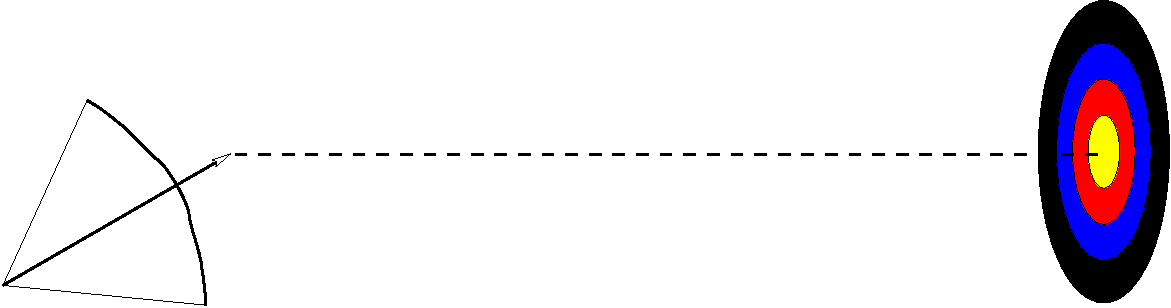
\includegraphics[width=0.6\textwidth]{./Figures/target.pdf}
\end{center}
\end{application}

For our modelling, we assume that the tip of the arrow is exactly level with the bullseye when it is loosed, cf. the sketch above. The target is 30 metres away. Then the height of the arrow when it hits the target is
\[h(\alpha,v) = -\frac{4414.5}{\cos^2(\alpha) \, v^2} + 30 \, \tan\alpha \:. \]
Here, $h=0$ corresponds to hitting the bullseye. There are different possibilities for defining a measurement of ``instability'', and Alice decides to use 
\[ f(\alpha,v) = h_{\alpha}^2 + 3 h_v^2 \]
since she finds controlling the velocity more difficult than controlling the angle. The symbols $h_\alpha$ and $h_v$ are the partial derivatives of $h$ and will be defined in the next section. After familiarising yourself with that concept, convince yourself that $f$ as defined above can be considered a measure of instability of\footnote{What does it mean for a derivative to be large at a point? It means that a small change of the variable will have a large effect!} $h$. In this chapter, we will learn how to minimise functions like $f$ (instability) under constraints like $h=0$ (hitting the bullseye). The optimal angle and velocity for Alice's target practice are
\[\alpha^* = 44.70^{\circ} \:,\quad v^* = 17.16 \tfrac{m}{s} \:. \]

The fact that those numbers do not agree with how archers usually shoot is due to our assumptions and our modelling: wind was neglected, it was assumed that initially the tip of the arrow and the bullseye are exactly level, that the archer can do the maths and control the angle and velocity exactly, etc. -- in the absence of these assumptions, a very strong shot almost directly aimed at the bullseye is the most straightforward option. However, understanding the above methods is a first step towards more complex real-life applications such as the design of mechanical machines.

\section{Multivariate Functions and Partial Derivatives}

\begin{definition}[Functions of Several Variables]
A \emph{function of two variables} is a rule $f$ that assigns to each pair $(x,y)$ in a set $D\subseteq\mathbb{R}^2$ a unique real number $f(x,y)$. The set $D$ is called the \emph{domain} of $f$ and also denoted $D(f)$. The \emph{range} of $f$ is the set of values it maps to,
\[
R(f) = \left\{ z \in \mathbb{R} \: | \: z = f(x,y)\text{~for some~}(x,y)\in D  \right\} \:.
\]
Similarly, a \emph{function of $n$ variables} is a rule $f$ that assigns a unique real number $f(x_1,x_2,\dots,x_n)$ to each $(x_1,x_2,\dots,x_n) \in D\subseteq\mathbb{R}^n$.
\end{definition}

\begin{remark}
\begin{enumerate}[(i)]
	\item Writing $z=f(x,y)$, we call $x$ and $y$ the independent variables, and $z$ the dependent variable. Functions of several variables are also called \emph{multivariate functions}.
	\item Unless specified otherwise, the domain is always the largest set of points $(x,y)$ at which the expression that defines $f$ can be evaluated.
	\item Functions of two variables can be visualised as surfaces/graphs in $\mathbb{R}^3$: The domain is a subset of the $xy$-plane and for $(x_0,y_0)$ in that domain, we mark a point of height $f(x_0,y_0)$ over/under $(x_0,y_0)$. That is, the point of the graph with $(x,y)$-coordinates $(x_0,y_0)$ will have $z$-coordinate $z_0=f(x_0,y_0)$.
	\item Restriction to lines in the domain is an important technique for working with multivariate functions, cf. part (iv) of the following set of examples.
\end{enumerate}
\end{remark}

\begin{example}
\label{expl:first_graphs}
\begin{enumerate}[(i)]
\item Draw the graph of $f(x,y) = x^2 + y^2$.\\
{\it Sol.:}
%\figbox{Graph of $f$ (paraboloid) with curves from parts (iv) and (v) (3D):}
\begin{center}
	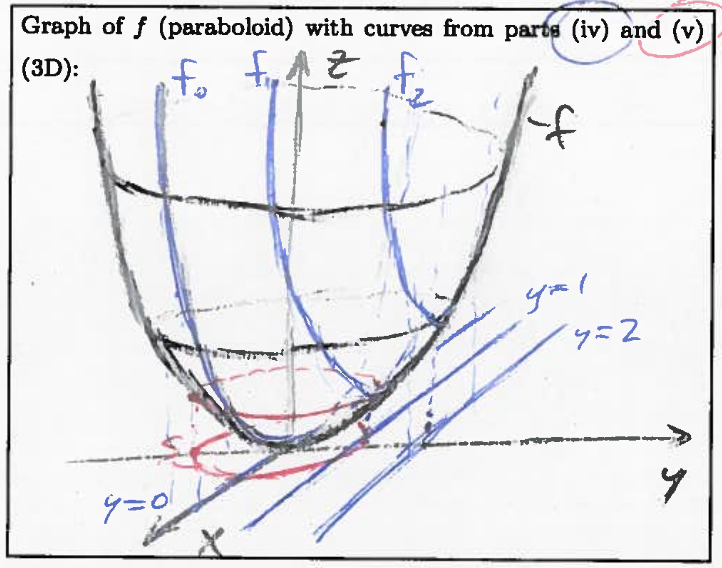
\includegraphics[width=0.6\textwidth]{./Figures/f301.png}
\end{center}
\item Find the domain and range of $g(x,y)= 1 + \sqrt{y-x^2}$.\\
{\it Sol.:}
The function $g$ is defined on the set
\[ D(g) = \left\{ (x,y) \in \mathbb{R}^2 \: | \: y \ge x^2 \right\} = \left\{ y \ge x^2 \right\} \:, \]
since we need $ y-x^2 \ge 0$ to be able to evaluate the square root. On this domain, the argument of the square root takes all non-negative real values $t\in[0,\infty)$, producing non-negative real numbers $\sqrt{t}\in[0,\infty)$. Therefore, the range is $R(g) = [1, \infty).$
\item Find the domain and range of $h(x_1,x_2,x_3)= \sin (x_1x_2+x_3)$.\\
{\it Sol.:}
The domain is $D = \mathbb{R}^3$ since $h$ can be evaluated at any $(x_1,x_2,x_3)$. The range of $h$ is $R = [-1,1]$.
\item Draw the graphs of the following one-variable functions
\begin{equation*}
\begin{split}
f_0(x) & = x^2 \:, \\
f_1(x) & = x^2 + 1 \:, \\
f_2(x) & = x^2 + 4 \:.
\end{split}
\end{equation*}
Where do these curves appear in the graph in (i)?\\
{\it Sol.:}
The functions $f_0,f_1,f_2$ are restrictions of $f(x,y)$ in (i) to the lines $y=0,y=1,y=2$. This can also be expressed as
\begin{equation*}
\begin{split}
f_0(x) & = f(x,0) = x^2 + 0^2 \:, \\
f_1(x) & = f(x,1) = x^2 + 1^2 \:, \\
f_2(x) & = f(x,2) = x^2 + 2^2 \:.
\end{split}
\end{equation*}
%\figbox{Graphs of $f_0,f_1,f_2$ (compare to graph (i); 2D):}
\begin{center}
	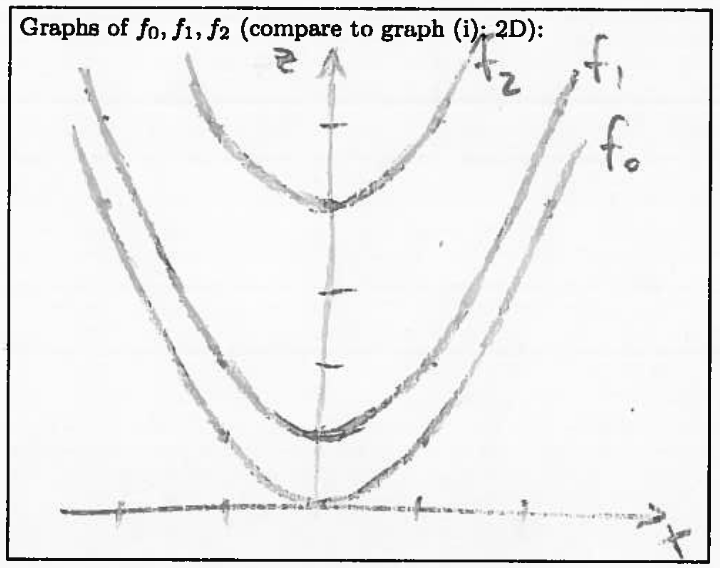
\includegraphics[width=0.6\textwidth]{./Figures/f302.png}
\end{center}
\item The domain of the function $f(x,y) = x^2 + y^2$ from (i) is $D(f)=\mathbb{R}^2$. Describe the subset $S$ of points in $D$ with $f(x,y)=1$.\\
{\it Sol.:} The equation
\[ x^2 + y^2 = 1 \]
defines a circle in the $xy$-plane:
%\figbox{Curve $S$ in $xy$-plane (compare to graph (i); 2D):}
\begin{center}
	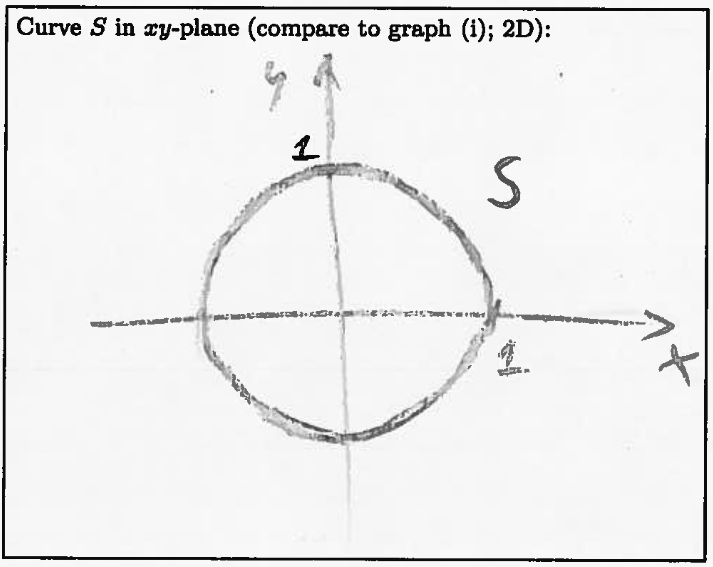
\includegraphics[width=0.6\textwidth]{./Figures/f303.png}
\end{center}
\end{enumerate}
\end{example}

\begin{definition}[Partial Derivatives]
For a function $f$ of two variables, the \emph{partial derivatives} with respect to $x$, respectively $y$, are the functions 	
\begin{equation*}
\begin{split}
\df{f}{x}(x,y) & = \lim_{h\to 0} \frac{f(x+h,y)-f(x,y)}{h} \:, \\
\df{f}{y}(x,y) & = \lim_{h\to 0} \frac{f(x,y+h)-f(x,y)}{h} \:.
\end{split}
\end{equation*}
We also write $f_x$ for $\df{f}{x}$ and $f_y$ for $\df{f}{y}$. Similarly for functions of more than two variables:
\begin{equation*}
\df{f}{x_j}(x_1,x_2,\dots,x_n) = \lim_{h\to 0}
\frac{f(x_1,x_2,\dots,x_{j-1},x_j+h,x_{j+1},\dots,x_n)-f(x_1,x_2,\dots,x_n)}{h} \:. \\
\end{equation*}
\end{definition}

\begin{example}
Find $f_x$ for the function $f(x,y) = 5x^2y^7$.\\
{\it Sol.:}
\begin{equation*}
\begin{split}
\df{f}{x}(x,y) & = \lim_{h\to 0}  \frac{f(x+h,y)-f(x,y)}{h} \\
& = \lim_{h\to 0}  \frac{5(x+h)^2y^7-5x^2y^7}{h} \\
& = 5y^7 \lim_{h\to 0} \frac{(x+h)^2 - x^2}{h} \\
& = 5y^7 \lim_{h\to 0} \frac{x^2+2hx+h^2 - x^2}{h} \\
& = 5y^7 \lim_{h\to 0} (2x+h) = 5(2x)y^7 = 10xy^7 \:.
\end{split}
\end{equation*}
The factor $2x$ in the last line is just the ordinary single-variable derivative of the factor $x^2$ of $f$. That is, the operator $\rfrac{\partial}{\partial x}$ differentiates the $x$-dependent part of $f$ in the usual way and treats terms that do not depend on $x$ as constants:
\begin{equation*}
\df{f}{x}(x,y) = \df{}{x} \left( 5x^2y^7\right) = 5 \, \df{}{x} \left( x^2\right) y^7 = 5(2x)y^7 = 10xy^7 \:.
\end{equation*}
\end{example}

\begin{example}
\begin{enumerate}[(i)]
	\item For $f = x^3 + y^5 - 2$, find $f_x$ and $f_y$.\\
	{\it Sol.:}
	\begin{equation*}
	\begin{split}
	f_x & = \df{}{x} \left( x^3 + y^5 - 2 \right) = 3x^2+0+0 = 3x^2 \:, \\
	f_y & = \df{}{y} \left( x^3 + y^5 - 2 \right) = 0+5y^4+0 = 5y^4 \:. 
	\end{split}
	\end{equation*}
	\item For $f=x^3+x^2y^3 -2 y^2$, find $f_x$ and $f_y$.\\
	{\it Sol.:}
	\begin{equation*}
	\begin{split}
	f_x & = \df{}{x} \left( x^3 \right) + \df{}{x} \left( x^2 \right)y^3 - 0 = 3x^2 +2xy^3 \:, \\
	f_y & = 0 + x^2 \df{}{y} \left( y^3 \right) - 2 \df{}{y}\left( y^2 \right) = 3x^2y^2 -4y \:. \\
	\end{split}
	\end{equation*}
\end{enumerate}
\end{example}

\begin{remark}
\begin{enumerate}[(i)]	
\item For a geometric interpretation, we consider the graph of a function $f$ of two variables, i.e. $z = f(x,y)$. Then $\rfrac{\partial z}{\partial x}$ is the slope on the surface ``when moving in the $x$ direction''. That is, $x$ is varied, $y$ is held constant, and we take note of the change of function values. Similarly, $\rfrac{\partial z}{\partial y}$ is the slope in the $y$ direction. 

As an intuitive example, consider a hiker climbing a mountain of the shape $z = 4-(x^2+y^2)$. 
%\figbox{``Steep mountain'' with hiker's position and paths in $x$ and $y$ direction (3D):}
\begin{center}
	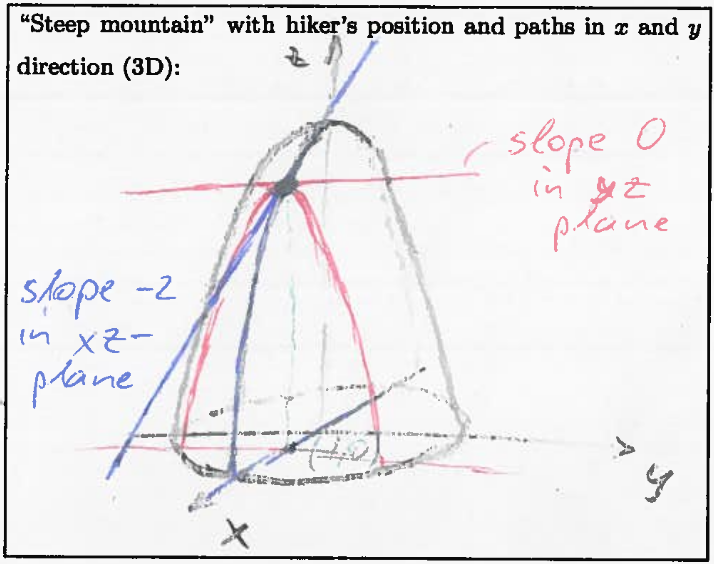
\includegraphics[width=0.6\textwidth]{./Figures/f304.png}
\end{center}
Suppose she checks her GPS and finds that her coordinates are $(x,y) = (1,0)$. The slopes at this point in both directions are
\begin{equation*}
\begin{split}
z_x(1,0) & = \df{}{x} \left( 4-(x^2+y^2) \right)_{|(x,y)=(1,0)} 
	= \left( -2x \right)_{|(x,y)=(1,0)} = -2 \:, \\
z_y(1,0) & = \df{}{y} \left( 4-(x^2+y^2) \right)_{|(x,y)=(1,0)} 
	= \left( -2y \right)_{|(x,y)=(1,0)} = 0 \:.
\end{split}
\end{equation*}
That is, there is no slope in the $y$ direction. The slope in the $x$ direction is negative, because the height decreases as $x$ increases (from where she stands, increasing $x$ would be moving away from the peak).
\item In order to be able to work with a larger set of functions -- not just sums of  products and powers of variables -- we extend the single-variable differentiation rules to the multivariate setting: The $x$-derivative of a product of functions is
\[ (fg)_x  = f_xg + fg_x \:, \]
that is, the product rule extends to partial derivatives without any changes. Similarly for $\rfrac{\partial}{\partial y}$. The quotient rule for a $y$-derivative is
\[ \left( \frac{f}{g} \right)_y = \frac{f_y g-f g_y}{g^2} \:. \]
\item In order to find partial derivatives of functions like
\[ f(x,y) = \sin(x+y^2) \:, \]
we also need to combine the chain rule for single-variable functions with partial derivatives. Note that the outer function, $h(t)=\sin(t)$, is a single-variable function. Let $c$ be a constant and review the following applications of the single-variable chain rule.
\begin{equation}
\label{eq:single-var_chain}
\begin{split}
\Df{}{t}\left(\sin(t+c)\right) & = \cos(t+c) \Df{}{t} (t+c) = \cos(t+c) \:,  \\
\Df{}{t}\left(\sin(c+t^2)\right) & = \cos(c+t^2) \Df{}{t} (c+t^2) = 2t\cos(c+t^2) \:.
\end{split}
\end{equation}
Now, the term $y^2$ looks like a constant to the operator $\rfrac{\partial}{\partial x}$. Similarly for $x$ and $\rfrac{\partial}{\partial y}$. We can thus apply the single-variable computations \eqref{eq:single-var_chain} to the two-variable function $f$ (in the first case, just replace $y^2$ with $c$):
\begin{equation*}
\begin{split}
f_x & = \df{}{x}\left(\sin(x+y^2)\right) = \cos(x+y^2) \df{}{x} (x+y^2) = \cos(x+y^2) \:,  \\
f_y & = \df{}{y}\left(\sin(x+y^2)\right) = \cos(x+y^2) \df{}{y} (x+y^2) = 2y\cos(x+y^2) \:.
\end{split}
\end{equation*}
This can be stated as
\[ \df{}{x} h(g(x,y)) = h'(g(x,y)) \cdot g_x(x,y) \:, \]
where $h$ is a single-variable function. Similarly for $\rfrac{\partial}{\partial y}$. Note that the $'$ is not ambiguous -- $h$ has only one variable, and $h'$ is the derivative with respect to (abbreviated: ``w.r.t'') that variable.
\end{enumerate}
\end{remark}

\begin{example}
\begin{enumerate}[(i)]
	\item The $y$-derivative of $f(x,y)=\e^{x^2+y^3}$ is found easily,
	\[ \df{}{y} \left( \e^{x^2+y^3} \right) 
	= \e^{x^2+y^3} \cdot \df{}{y}(x^2+y^3) = 3y^2 \, \e^{x^2+y^3} \:, \]
	and we can verify this result with the following alternative approach.
	\begin{equation*}
	\begin{split}
	\df{}{y} \left( \e^{x^2+y^3} \right) & = \df{}{y} \left( \e^{x^2}\e^{y^3} \right) = \e^{x^2} \df{}{y} \left( \e^{y^3} \right) \\
	& = \e^{x^2} \Df{}{y} \left( \e^{y^3} \right) = \e^{x^2} \e^{y^3} 3y^2 
	= 3y^2 \, \e^{x^2+y^3} \:. 
	\end{split}
	\end{equation*}
	Here, the ``$\partial$'' was changed to a ``$\d$'' to emphasise that in this approach, an ordinary derivative was taken, i.e., a derivative of a single-variable expression.
	\item 
	\[\begin{split}
	 \df{}{x}\left( \frac{\sin x \cos y }{x+y}\right) 
	& = \frac{\df{}{x}\Big(\sin x \cos y\Big) (x+y) - (\sin x \cos y)\df{}{x}\Big(x+y\Big)}{(x+y)^2} \\
	& = \frac{\cos y \left[ \cos x \cdot (x+y) - \sin x \right]}{(x+y)^2} 
	\end{split} \]
	\smallskip
\end{enumerate}
\end{example}

\begin{definition}[Higher-Order Partial Derivatives]
The \emph{second-order partial derivatives} with respect to $x$ and $y$ of a function $f$ of two variables are written
\begin{equation*}
\begin{split}
\ddf{f}{x} & = \df{}{x}\left( \df{f}{x}\right) , \\
\ddf{f}{y} & = \df{}{y}\left( \df{f}{y}\right) ,
\end{split}
\end{equation*}
and can also be denoted $f_{xx}$ and $f_{yy}$. We further have \emph{mixed} second-order derivatives:
\begin{equation*}
\begin{split}
\dff{f}{x}{y} & = \df{}{x}\left( \df{f}{y}\right) , \\
\dff{f}{y}{x} & = \df{}{y}\left( \df{f}{x}\right) .
\end{split}
\end{equation*}
Similarly for functions of more than two variables and for higher-order derivatives; e.g.,
\[ f_{xyyz} =\frac{\partial^4 f}{\partial x \partial y \partial y \partial z} 
		   = \df{}{x}\left(\df{}{y}\left(\df{}{y}\left(\df{f}{z}\right)\right)\right) \]
is a fourth-order derivative of a three-variable function $f=f(x,y,z)$.
\end{definition}

\begin{example}
\begin{enumerate}[(i)]
	\item
	For \[ f(x,y) = 2x^9y^5 \:, \] find all partial derivatives of order up to 2.\\
	{\it Sol.:}
	\begin{equation*}
	\begin{split}
	f & = 2x^9y^5 \:, \\
	f_x & = 2(9x^8)y^5=18x^8y^5 \:, \\
	f_y & = 2x^9(5y^4)=10x^9y^4 \:, \\
	f_{xx} & = \df{}{x} \left( 18x^8y^5 \right)=18(8x^7)y^5=144x^7y^5 \:, \\
	f_{yy} & = \df{}{y} \left( 10x^9y^4 \right)=10x^9(4y^3)=40x^9y^3 \:, \\
	f_{xy} & = \df{}{x} \left( 10x^9y^4 \right)=10(9x^8)y^4=90x^8y^4 \:, \\
	f_{yx} & = \df{}{y} \left( 18x^8y^5 \right)=18x^8(5y^4)=90x^8y^4 \:.
	\end{split}
	\end{equation*}
	\item
For \[f(x,y) = x^2 + 3xy - y^2 + 7x -4 y +2 \:, \] find \emph{all} partial derivatives.\\
{\it Sol.:}
\begin{equation*}
\begin{split}
f & = x^2+3xy-y^2+7x-4y+2 \:, \\
f_x & =  2x+3y+7 \:, \\
f_y & =  3x-2y-4 \:, \\
f_{xx} & = 2 \:, \\
f_{yy} & = -2 \:, \\
f_{xy} & = 3 \:, \\
f_{yx} & = 3 \:.
\end{split}
\end{equation*}
Since all the second-order derivatives are constant, all derivatives of higher order are zero,
\[ \frac{\partial^k f}{\partial \dots} = 0 \qquad \text{for~}k>2 \:. \]
	\item
	For \[ f(x,y) = x\, \cos(xy^2) \:, \] find all partial derivatives of order up to 2.\\
	{\it Sol.:}
	\begin{equation*}
	\begin{split}
	f & = x \cos(xy^2) \:, \\
	f_x & = \cos(xy^2) - xy^2 \sin(xy^2) \:, \\
	f_y & = -2x^2y \sin(xy^2) \:, \\
	f_{xx} & = -2y^2 \sin(xy^2) - xy^4 \cos(xy^2) \:, \\
	f_{yy} & = -2x^2 \sin(xy^2) - 4x^3y^2 \cos(xy^2) \:, \\
	f_{xy} & = -4xy \sin(xy^2) - 2x^2y^3 \cos(xy^2) = f_{yx} \:.
	\end{split}
	\end{equation*}
\end{enumerate}
\end{example}

\begin{remark}
In all of the previous examples, we had $f_{xy}=f_{yx}$. The following theorem states that this is not a coincidence -- it is always true as long as certain technical conditions are satisfied. Those conditions are met for the functions considered in this book, hence we can always work with the conclusion of the following theorem. However, be aware that there are functions that do not meet its requirements.
\end{remark}

\begin{theorem}[Schwarz's Theorem or Clairaut's Theorem]
\label{thm:schwarz}
Consider a function $f=f(x,y)$ and a point $(a,b)$ in its domain. If the functions $f_{xy}$ and
$f_{yx}$ are both continuous at $(a,b)$, then
\[f_{xy}(a,b)=f_{yx}(a,b) \:. \]
\end{theorem}

\begin{remark}
\texttt{Short remark on continuity for multivariate functions; or leave it -- depending whether 1D continuity is covered in chapter 1.}
\end{remark}

\begin{exercise}
\begin{enumerate}[(i)]
	\item Restrict the function $f(x,y)=xy$ to the lines $x=0$, $y=0$, $y=x$, $y=-x$. Hence draw the graph of\footnote{We have
	\[ f(x,x)=x^2\:, \quad f(x,-x) = -x^2 \:. \]
	That is, there is a parabola ``sitting'' on the line $y=x$ of the $xy$-plane and an upside-down parabola ``hanging'' under the line $y=-x$. The full graph looks like a saddle. You can use software to help visualising such functions; e.g., enter \texttt{plot x*y} in WolframAlpha. Note that, even though this is a curved surface, you can form it with straight lines (e.g., with mikado sticks) since the restriction of the graph to any $y=c$ is a line.} $f$.
	\item Find $f_x,f_y,f_{xx},f_{xy},f_{yy},f_{yx}$ for the functions\footnote{The $xy$ derivatives of the three functions are
	\[ 2x+12x^2y^3 \:, \quad \e^x \:, \quad -\sin x \, \tfrac{1}{y} \:, \]
	and we always have $f_{xy}=f_{yx}$. You can use software to check your results; e.g., \texttt{partial derivatives of \ldots} in WolframAlpha. Use such commands only to support your studies though -- do not rely on software!}
	\begin{enumerate}[(a)]
		\item $f(x,y) = x^2y+x^3y^4 + 7y \:;$
		\item $f(x,y) = y\,\e^x \:;$
		\item $f(x,y) = \cos x \ln y \:.$
	\end{enumerate}
	\item Find $f_x,f_y,f_{xx},f_{xy},f_{yy},f_{yx}$ for the functions\footnote{The $xy$ derivatives of the three functions are
		\[ \cos(xy+y^3) - y (x+3x^2) \sin(xy+y^3) \:, \quad
		-4xy - 2xy \ln xy \:, \quad 
		\tfrac{2y(1+x^2+y^2)^2-4xy(1+x^2+y^2)(2x)}{(1+x^2+y^2)^4} \:. \]
		(If you don't quite get those expressions, you may have forgotten to apply the product rule.)}
	\begin{enumerate}[(a)]
		\item $f(x,y) = \sin \left( xy + y^3 \right) \:;$
		\item $f(x,y) = \frac{x^2y^2}{2}-x^2y^2 \ln (xy) \:;$
		\item $f(x,y) = \frac{x}{1+x^2+y^2} \:.$
	\end{enumerate}
	\item Find the domain and the range of\footnote{You can check your domain with a WolframAlpha command of the form \texttt{plot ... >= 0}.} $f(x,y) =\sqrt{ 2 \sin x \sin y}$. 
		\item Let $D\subseteq\mathbb{R}^2$ be the open disk of radius $1$, $D = \{x^2 + y^2 < 1\}$. Define a function that is defined for $(x,y) \in D$, and another function that is defined on the \emph{complement} of $D$,
	\[D^c = \mathbb{R}^2 \setminus D = \{x^2+y^2 \geq 1 \} \]
	(read this as ``all points outside of $D$'')\footnote{For example: $\ln(1-x^2-y^2)$ and $\sqrt{x^2+x^2-1}$\:.}.
	\item Verify that
	\begin{enumerate}[(a)]
		\item $y(t,x) = \e^{-kn^2t}\sin(nx) \:$ satisfies $\: y_t=ky_{xx} \:;$
		\item $r(x,y,z) = \sqrt{x^2+y^2+z^2} \:$ satisfies
		$\: r_{xx}+r_{yy}+r_{zz} = \tfrac{2}{r} \:.$
	\end{enumerate}
	\item Find \emph{all} partial derivatives of\footnote{Use Theorem~\ref{thm:schwarz} to justify that your answer can be given in the form \[\frac{\partial^n}{\partial y^n} \frac{\partial^m f}{\partial x^m}=\dots \:, \] i.e. it can be assumed that $x$-derivatives are taken first.} $f(x,y) = \e^{2x+3y}$.
	\item Consider the function $f(x,y)=x^2(1-x^2)-y^2$. Find all points for which both the $x$- and the $y$-derivative is equal to zero. That is, find $(x_0,y_0)$ with\footnote{Setting both partial derivatives equal to zero gives you a (non-linear) system of two equations; solving it should lead to three points.} $f_x(x_0,y_0)=f_y(x_0,y_0)=0$.
\end{enumerate}
\end{exercise}


\section{Chain Rule and Implicit Differentiation}

\begin{remark}
\label{rem:composition}
\emph{Curves} in the $xy$-plane can be parametrised by writing $x$ and $y$ as single-variable functions of a third variable, usually $t$ (think of it as ``time''):
\[ (x,y) = (x(t),y(t)) \:. \]
We denote such curves $\gamma$,
\begin{equation*}
\begin{split}
\gamma \: : \: \mathbb{R} & \: \rightarrow \: \mathbb{R}^2 \\
t & \: \mapsto \: \gamma(t) = \left(x(t),y(t)\right) \:.
\end{split} 
\end{equation*}
A given function $f=f(x,y)$ can then be restricted to $\gamma$ -- this is carried out formally via a composition : define the single-variable function $F$ as
\[F(t) = \left(f\circ\gamma\right) (t) = f(\gamma(t)) = f(x(t),y(t)) \:. \]
Finding the derivative of $F$ is now an important and applicable task.

The distinction $f \leftrightarrow F$ is often not made to simplify notation. That is, the single-variable function of $t$ may be called $f$ as well. This reduces the number of function names needed to write out a computation, but it also carries potential for confusion since the symbol ``$f$'' would then used for two different mathematical objects. 
\end{remark}

\begin{example}
\label{expl:chainruleI}
\begin{enumerate}[(i)]
	\item Draw the curves
		\begin{equation*}
		\begin{split}
		\gamma_1 \: & : \quad (x(t),y(t)) = (t,t) \:, \\
		\gamma_2 \: & : \quad (x(t),y(t)) = (3\cos t,3\sin t) \:, \\
		\gamma_3 \: & : \quad (x(t),y(t)) = (t,1-t^2) \:, 
		\end{split}
		\end{equation*}
		and highlight the point corresponding to $t=0$ in each of them. \\
		{\it Sol.:} 
		%\figbox{The curves $\gamma_1,\gamma_2,\gamma_3$ (2D):}
		\begin{center}
			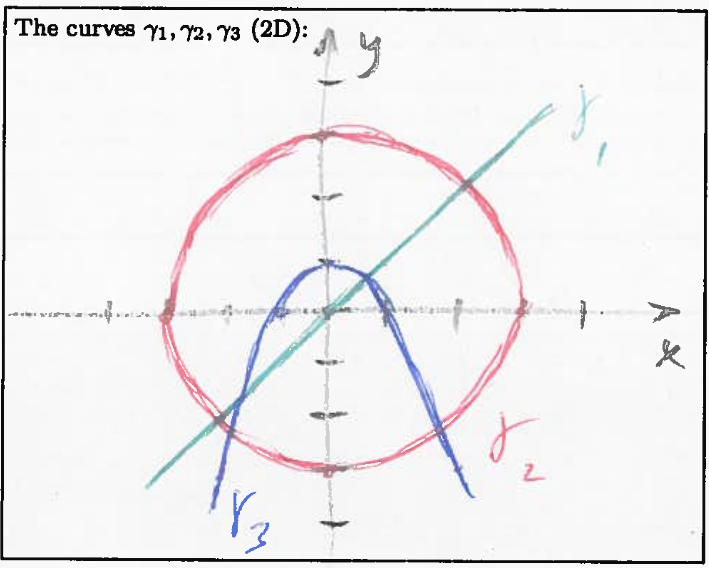
\includegraphics[width=0.6\textwidth]{./Figures/f305.png}
		\end{center}
	\item Consider the functions
		\begin{equation*}
		\begin{split}
		f_1 \: & : \quad f_1(x,y) = x-y \:, \\
		f_2 \: & : \quad f_2(x,y) = x^2+y^2 \:, \\
		f_3 \: & : \quad f_3(x,y) = \ln (3+x^2-y) \:, 
		\end{split}
		\end{equation*}
		and find the three single-variable functions $F_i=f_i\circ\gamma_i$.\\
		{\it Sol.:} 
		\begin{equation}
		\label{eq:chainruleI}
		\begin{split}
		F_1(t) & = \left(f_1\circ\gamma_1\right)(t) = f_1(t,t) = t-t = 0 \:, \\
		F_2(t) & = \left(f_2\circ\gamma_2\right)(t) = f_2(3\cos t, 3\sin t) 
		= (3\cos t)^2 +  (3\sin t)^2 = 9 \:, \\
		F_3(t) & = \ln \left( 3 + t^2 - (1-t^2) \right) = \ln \left( 2 + 2t^2\right) = \ln 2 + \ln\left(1+t^2\right).
		\end{split}
		\end{equation}
\end{enumerate}
\end{example}

\begin{theorem}[Chain Rule I]
\label{thm:CRI}
Let $f$ and $F$ be as in Remark~\ref{rem:composition}. Then
\[ \Df{F}{t} = \df{f}{x} \Df{x}{t} + \df{f}{y} \Df{y}{t} \:. \]
\end{theorem}

\begin{example}
\label{expl:chain_rule_i}
\begin{enumerate}[(i)]
	\item The derivatives of the functions $F_i$ in \ref{expl:chainruleI} are
\begin{equation*}
\begin{split}
\Df{F_1}{t} & = \df{f_1}{x} \Df{x}{t} + \df{f_1}{y} \Df{y}{t} 
= \df{(x-y)}{x} \Df{t}{t} + \df{(x-y)}{y} \Df{t}{t} = 1 \cdot 1 + (-1)\cdot 1 = 0 \:, \\
\Df{F_2}{t} & 
= 2x(t) \cdot (-3\sin t) + 2y(t) \cdot 3\cos t = -6 \cos t \sin t + 6 \sin t \cos t = 0 \:,  \\
\Df{F_3}{t} & = \frac{2x}{3+x^2-y} \cdot 1 + \frac{-1}{3+x^2-y} \cdot (-2t) 
= \frac{4t}{2+2t^2} = \frac{2t}{1+t^2} \:.
\end{split}
\end{equation*}
Alternatively, these derivatives could have been found by directly differentiating the functions $F_i=F_i(t)$ in \eqref{eq:chainruleI}. However, the chain rule allowed us to find the derivatives without using the explicit expressions of $t$ on the right-hand sides of \eqref{eq:chainruleI}, which is often very helpful.
	\item We now present an example in the simplified notation mentioned at the end of Remark~\ref{rem:composition}: For $f=x^2 y + 3x y^4$, $x=\sin 2 t$, $y= \cos t$,  find $\rfrac{\d f}{\d t}$ at $t=0$.
	{\it Sol.:}
\[ \Df{f}{t} = \df{f}{x} \Df{x}{t} + \df{f}{y}\Df{y}{t} 
= (2xy+ 3y^4)(2\cos 2t)+(x^2+12 xy^3)(-\sin t) \:. \]
The expressions containing the variable $t$ can be evaluated at $t=0$ directly. The other expressions we evaluate at the $x$ and $y$ values at $t=0$ : $x(0)=0$, $y(0)=1$. Therefore, the $t$-derivative of $f$ at $t=0$ is
\[ \Df{f}{t}(0) = 3\cdot 2 + 0 \cdot 0 = 6 \:. \]

To give this derivative a geometric interpretation, think of a hiker walking along the path $(x(t),y(t))$ in the ``mountain range'' that is given by the graph of $f$. Then our computations show that at time $t=0$, he will be climbing at a rate of six height units per time unit.
\end{enumerate}
\end{example}

\begin{remark}
\label{rem:transformations}
\emph{Changes of variables} in the $xy$-plane can be realised by writing $x$ and $y$ as functions of \emph{two} other variables,
\[ (x,y) = (x(s,t),y(s,t)) \:. \]
Given a function $f=f(x,y)$, one can then define a new function $F$ that has the same values as $f$, but is written out in term of $s$ and $t$ :
\[F(s,t) = f(x(s,t),y(s,t)) \:. \]
These changes of variables are quite useful -- for example, we will use them to solve differential equations in chapter \ref{ch:de} -- and it is important to be able to understand the relation of the partial derivatives of $f$ and $F$.

As in Remark~\ref{rem:composition}, the distinction $f \leftrightarrow F$ is sometimes not made, and the function of the new variables may be called $f$ as well. Again, this simplifies the notation but also carries potential for confusion. 
\end{remark}

\begin{theorem}[Chain Rule II]
\label{thm:CRII}
For $s,t,x,y,f,F$ as in Remark~\ref{rem:transformations}, we have
\begin{equation*}
\begin{split}
\df{F}{s} & = \df{f}{x}\df{x}{s} + \df{f}{y}\df{y}{s} \:, \\
\df{F}{t} & = \df{f}{x}\df{x}{t} + \df{f}{y}\df{y}{t} \:.
\end{split}
\end{equation*}
\end{theorem}

\begin{example}
\label{expl:chain_rule_ii}
\begin{enumerate}[(i)]
	\item Consider the function $f(x,y)=x-y$ and the change of variables 
	\[x(s,t)=s+t \:, \qquad y(s,t)=s-t \:. \]
	For $f$ in the new variables, i.e. $F(s,t)=f(x(s,t),y(s,t))$, we have partial derivatives 
	\begin{equation*}
	\begin{split}
	\df{F}{s} & = \df{f}{x}\df{x}{s} + \df{f}{y}\df{y}{s} = 1 \cdot 1 + (-1) \cdot 1 = 0 \:, \\
	\df{F}{t} & = \df{f}{x}\df{x}{t} + \df{f}{y}\df{y}{t} = 1 \cdot 1 + (-1) \cdot (-1) = 2 \:.
	\end{split}
	\end{equation*}
	As in the examples for derivatives along curves, the derivatives can be checked by explicitly writing out the function $F$ in terms of $s$ and $t$ :
	\[ F(s,t) = f(x,y) = x-y = (s+t)-(s-t) = 2t \:, \]
	which has the partial derivatives that were obtained above.
	\item Consider the paraboloid $f(x,y)=x^2+y^2$ and the change of variables
	\begin{equation}
	\label{eq:polar_coords}
	x(r,\theta)=r\cos\theta, \qquad y(r,\theta)=r\sin\theta \:.
	\end{equation}
	The partial derivatives of $F(r,\theta)=f(x,y)$ are
	\begin{equation*}
	\begin{split}
	\df{F}{r} & = \df{f}{x}\df{x}{r} + \df{f}{y}\df{y}{r} 
	= 2x \cdot \cos\theta + 2y \cdot \sin\theta 
	= 2r \left( \cos^2\theta + \sin^2\theta \right) = 2r \:, \\
	\df{F}{\theta} & = \df{f}{x}\df{x}{\theta} + \df{f}{y}\df{y}{\theta} 
	= 2r\cos\theta \cdot (-r\sin\theta) + 2r\sin\theta \cdot r\cos\theta = 0 \:.
	\end{split}
	\end{equation*}
	Again, we check these derivatives by explicitly writing out the function $F$ :
	\[ F(r,\theta) = f(x,y) = x^2+y^2 = r^2 \left( \cos^2\theta + \sin^2\theta \right) = r^2 \:, \]
	which confirms the partial derivatives that were found via chain rule II.
	
	The change of variables \eqref{eq:polar_coords} is the very important change to \emph{polar coordinates}. \texttt{Adjust this paragraph depending on whether polar coordinates are reviewed in the foundations chapter.}
	
	\item Let $g(s, t)=f(s^2-t^2, t^2-s^2)$, where $f$ is an arbitrary differentiable function. Show that $g$ satisfies
	\[ t\df{g}{s} + s \df{g}{t}=0 \:. \]
	{\it Sol.:}
	Let $ x=s^2-t^2, y=t^2-s^2$. Then,
	\begin{equation*}
	\begin{split}
	\df{g}{s} & = \df{f}{x} \df{x}{s} + \df{f}{y} \df{y}{s}=f_x \cdot 2s + f_y \cdot (-2s) \:, \\
	\df{g}{t} & = \df{f}{x} \df{x}{t} + \df{f}{y} \df{y}{t}=f_x \cdot (-2t) + f_y \cdot 2t \:.
	\end{split}
	\end{equation*}
	Therefore
	\[ t\df{g}{s} + s \df{g}{t}=0 \:. \]
	\item As in the examples \ref{expl:chain_rule_i} for chain rule I, we now present an example in simplified notation, where the function in the new variables is not given a new name. Consider the expression
	\begin{equation}
	\label{eq:first_pde_trafo}
	3\ddf{u}{x} +\frac12 \dff{u}{x}{y} -\frac12 \ddf{u}{y} 
	\end{equation}
	for the function $u=u(x,y)$, and rewrite it in terms of the new variables $\xi$ (``xi'') and $\eta$ (``eta'') defined as 
	\[ \xi=x+3y \:, \quad \eta=x-2y \:. \]
	{\it Sol.:} Chain rule II allows to rewrite the derivatives of $u$ with respect to $x$ and $y$ as derivatives w.r.t. $\xi$ and $\eta$ :
	\begin{equation*}
	\begin{split}
	\df{u}{x} &= \df{u}{\xi} \df{\xi}{x} + \df{u}{\eta} \df{\eta}{x}
	 = \df{u}{\xi} \cdot 1 + \df{u}{\eta} \cdot 1 = u_{\xi} + u_{\eta} \:, \\
 	\df{u}{y} &= \df{u}{\xi} \df{\xi}{y} + \df{u}{\eta} \df{\eta}{y}
	 = \df{u}{\xi} \cdot 3 + \df{u}{\eta} \cdot \left( -2 \right) 
	 = 3u_{\xi} - 2 u_{\eta} \:.
	 \end{split}
	\end{equation*}
	These formulas for the first-order derivatives of $u$ are only intermediate steps in our computation -- we need the second-order derivatives appearing in \eqref{eq:first_pde_trafo}: 
	\begin{equation*}
	\begin{split}
	\ddf{u}{x} & = \df{}{x}\left( \df{u}{x} \right)
		= \df{}{x} \left( u_{\xi} + u_{\eta} \right)
		= \df{u_{\xi}}{x} + \df{u_{\eta}}{x} \\
		& = \df{u_{\xi}}{\xi} \df{\xi}{x} + \df{u_{\xi}}{\eta} \df{\eta}{x}
		\: + \: \df{u_{\eta}}{\xi} \df{\xi}{x} + \df{u_{\eta}}{\eta} \df{\eta}{x} 
		 = u_{\xi\xi} + u_{\eta\xi} + u_{\xi\eta} + u_{\eta\eta} \:.
	\end{split}
	\end{equation*}
	Recalling Theorem~\ref{thm:schwarz}, we obtain
	\[ \ddf{u}{x} =  u_{\xi\xi} + 2 u_{\xi\eta} + u_{\eta\eta} \:. \]
	The second-order derivative w.r.t. $y$ is 
	\begin{equation*}
	\begin{split}
	\ddf{u}{y} &= \df{}{y}\left( 3u_{\xi} - 2 u_{\eta} \right)
	= 3\df{u_{\xi}}{y} -2 \df{u_{\eta}}{y} \\
	&= 3 \left( \df{u_{\xi}}{\xi} \df{\xi}{y} + \df{u_{\xi}}{\eta} \df{\eta}{y} \right)
-2 \left( \df{u_{\eta}}{\xi} \df{\xi}{y} + \df{u_{\eta}}{\eta} \df{\eta}{y} \right) \\
	&= 3\df{u_{\xi}}{\xi} \cdot 3 + 3\df{u_{\xi}}{\eta} \cdot \left( -2 \right)
	-2 \df{u_{\eta}}{\xi} \cdot 3
	-2 \df{u_{\eta}}{\eta} \cdot \left( -2 \right) \\
	&= 9 u_{\xi\xi} -12 u_{\xi\eta} + 4 u_{\eta\eta} \:.
	\end{split}
	\end{equation*}
	The mixed second-order derivative,
	\[ u_{xy} = 3 u_{\xi\xi} + u_{\xi\eta} - 2 u_{\eta\eta} \:, \]
	is obtained similarly. 
	This allows to write out \eqref{eq:first_pde_trafo} in terms of $\xi$ and $\eta$ :
	\begin{equation*}
	\begin{split}
	3\ddf{u}{x} & +\frac12 \dff{u}{x}{y} -\frac12 \ddf{u}{y} \\
	&= 3 \left[ u_{\xi\xi} + 2 u_{\xi\eta} + u_{\eta\eta} \right] 
	+\frac12 \left[ 3 u_{\xi\xi} + u_{\xi\eta} - 2 u_{\eta\eta} \right] 
	-\frac12 \left[ 9 u_{\xi\xi} - 12 u_{\xi\eta} + 4 u_{\eta\eta} \right] \\
	&= 0 \cdot u_{\xi\xi} + \left( 6 + \frac12 + 6 \right) \cdot u_{\xi\eta}
	+ 0 \cdot u_{\eta\eta} = \frac{25}{2} u_{\xi\eta} \:.
	\end{split}
	\end{equation*}
	Later, in Section \ref{sec:pdes}, we will use computations of this kind to solve a certain type of differential equation.
\end{enumerate}
\end{example}

\begin{definition}[Level Sets]
Given a function $f$ of $n$ variables and a constant $c$ in the range of $f$, the set of points in the domain of $f$ with
\[ f = c \]
is called a \emph{level set} of $f$. That is, a level set of $f$ is of the form
\[  \left\{ (x,y)\in\mathbb{R}^2 \: | \: f(x,y)=c \right\}\:.\]
\end{definition}

\begin{remark}
\begin{enumerate}[(i)]
	\item Level sets usually have one dimension less than the domain of the function. For example, the function $f(x,y) = x^2 + y^2$ is defined on the $xy$-plane, $\mathbb{R}^2$, which is two-dimensional. We have seen in Example~\ref{expl:first_graphs} that the condition
	\[ f(x,y) = x^2 + y^2 = 1 \]
	describes a curve, i.e. a one-dimensional object, namely the circle of radius $1$. In fact, $f(x,y)=x^2+y^2=c$ describes a one-dimensional object for any $c>0$. This may not work for all values of $c$ though: the only solution to $f=0$ is the point $(x,y)=(0,0)$, and points are considered zero-dimensional. The equation $f=c$, where $c<0$, has no solutions at all.
	
	Similarly, consider the function $f(x,y,z) = x^2 + y^2 + z^2$. It is defined in the three-dimensional space $\mathbb{R}^3$, and its level sets $f=c$ for $c>0$ are two-dimensional objects: spheres of radius $\sqrt{c}$ (the surfaces of the balls of radius $\sqrt{c}$ centred at the origin of the coordinate system).
	\item Considering $x$ and $y$ independent variables, we have
	\[ \df{y}{x} = 0 \]
	(the $x$-derivative of the function $g(x,y)=y$ is zero, since $g$ does not depend on $x$). 
	
	Now consider a level set $f(x,y)=c$. Under the constraint $f(x,y)=c$, the variables cannot both move freely any more. Such a level set is one-dimensional by the previous remark, i.e. a curve, and we can use $x$ as a parameter for it. That is, we let $x$ vary freely (independent variable) and then $y$ is determined (not independent any more) by the choice of $x$.
	
	For example, requiring $f_1 = 0$ in~\ref{expl:chainruleI} gives $y(x) = x$, and $f_3=\ln(2)$ gives $y(x)=1+x^2$.
\end{enumerate}
\end{remark}

\begin{theorem}[Implicit Differentiation]
\label{thm:impl_diff}
If the independent variable $y$ of the $xy$-plane $(x,y)\in\mathbb{R}^2$ is turned into a dependent variable $y=y(x)$ via a condition $f(x,y)=c$ (as in (ii) of the previous remark), then
\[ \Df{y}{x} = -\frac{f_x}{f_y} \:. \]
Similarly in $\mathbb{R}^3$: If the independent variable $z$ of $(x,y,z)\in\mathbb{R}^3$ is turned into a dependent variable $z=z(x,y)$ via a condition $f(x,y,z)=c$, then
\begin{equation*}
\begin{split}
\df{z}{x} = -\frac{f_x}{f_z} \:, \\
\df{z}{y} = -\frac{f_y}{f_z} \:. 
\end{split}
\end{equation*}
\end{theorem}

\begin{proof} Differentiating the condition $f(x,y(x))=c$ with respect to $x$ gives
\begin{equation}
\label{eq:pid1}
\Df{c}{x} = 0
\end{equation}
on the right-hand side. On the left-hand side, we use chain rule I to obtain
\begin{equation}
\label{eq:pid2}
\Df{f(x,y(x))}{x} = \df{f(x,y)}{x}\Df{x}{x} + \df{f(x,y)}{y}\Df{y}{x} \:.
\end{equation}
Note that here, $f$ appears as a function of one independent variable on the left, and as a two-variable function on the right. Since $\rfrac{\d x}{\d x} = 1$, combining~\eqref{eq:pid1} and~\eqref{eq:pid2} leads to the claimed formula for $\rfrac{\d y}{\d x}$.

Similarly, we differentiate the condition $f(x,y,z(x,y))=c$ with respect to $x$ and $y$,
\begin{equation*}
\begin{split}
\df{f(x,y,z(x,y))}{x} & = \df{f}{x}\df{x}{x} + \df{f}{y}\df{y}{x} +\df{f}{z}\df{z}{x} 
= f_x \cdot 1 + f_y \cdot 0 +f_z \cdot \df{z}{x} = 0 \:, \\
\df{f(x,y,z(x,y))}{y} & = \df{f}{x}\df{x}{y} + \df{f}{y}\df{y}{y} +\df{f}{z}\df{z}{y} 
= f_x \cdot 0 + f_y \cdot 1 +f_z \cdot \df{z}{y} = 0 \:,
\end{split}
\end{equation*}
to derive the other formulas stated in the theorem. The terms with $\rfrac{\partial y}{\partial x}$ and $\rfrac{\partial x}{\partial y}$ drop out by the previous remark. Here, $f$ appears as a two-variable function on the left and as a three-variable function in the other expressions.
\end{proof}
	
\begin{example}
\label{expl:impl_diff}
\begin{enumerate}[(i)]
	\item Find $\rfrac{\d y}{\d x}$ if $ x^3+y^3=6xy$.\\
	{\it Sol.:}
	\[ f(x,y)=x^3 + y^3 - 6xy = 0	
		\quad \Longrightarrow \quad \Df{y}{x} = -\frac{f_x}{f_y}= -\frac{3x^2-6y}{3y^2-6x} \:. \]
	\item Find $\tfrac{\partial z}{\partial x}$, $\tfrac{\partial z}{\partial y}$, $\tfrac{\partial^2 z}{\partial x \partial y}$, where $z=z(x,y)$ is defined by the equation
	\[ x+y-z=\e^z \:. \]
	{\it Method 1:} For $f(x,y,z)=x+y-z-\e^z$, we have
	\[f_x = \df{f}{x} = 1, \quad f_y= \df{f}{y} = 1, \quad
	f_z = \df{f}{z} = -1-\e^z \:. \]
	By Theorem~\ref{thm:impl_diff}, 
	\begin{equation*}
	\begin{split}
	\df{z}{x} & = - \frac{f_x}{f_z}= \frac{1}{1+\e^z} \:,\\
	\df{z}{y} & = - \frac{f_y}{f_z}= \frac{1}{1+\e^z} \:,
	\end{split}
	\end{equation*}
	and then, using the single-variable chain rule,
	\begin{equation*}
	\begin{split}
	\dff{z}{x}{y} & = \df{}{x} \left( \frac{1}{1+\e^z} \right) 
	= - \frac{1}{(1+\e^z)^2} \df{}{x} \left( \e^z \right) \\
	& = - \frac{\e^z}{(1+\e^z)^2} \df{}{x} \left( z \right)	= - \frac{\e^z}{(1+\e^z)^3} \:.
	\end{split}
	\end{equation*}
	{\it Method 2:} Differentiating both sides of $x+y-z=\e^z$ with respect to $x$ gives
	\[ 1 - \df{z}{x} = \e^z \df{z}{x} \:. \]
	Solving this for $z_x$, we find the same derivative as before.
	
	The two computations are very closely related -- Method~2 was presented to show that a more flexible approach can be used as well.
	\item For $z=u^v$, where $u=\sin x$ and $v=\cos x$, find $\rfrac{\d z}{\d x}$. \\
	{\it Sol.:} The chain rule for $z=z(x)$ reads
	\[
	\Df{z}{x} =\df{z}{u} \df{u}{x} + \df{z}{v} \df{v}{x}
	\:. \]
	The partials of $z = z (u,v)$ are
	\[
	\df{z}{u} = v u^{v-1}, \quad \df{z}{v}= u^v \ln u
	\:, \]
	and therefore
	\[
	\Df{z}{x} = v u^{v-1} \cos x - u^v \ln u \cdot \sin x
	=(\sin x)^{\cos x -1}  \cos^2 x -   \ln (\sin x) \cdot (\sin x)^{\cos x +1}
	\:. \]
	\item (Logarithmic Differentiation) Find $\rfrac{\partial z}{\partial x}$, $\rfrac{\partial z}{\partial y}$  for
	\begin{equation}
	\label{eq:symmetric_z}
	z=(x^2y+xy^2)^{\cos(xy)} \:.
	\end{equation} 
	{\it Sol.:}
	The idea for dealing with the function in the power on the right is to use the rule $\ln(a^p)=p\ln(a)$ for logarithms. If $a=b$, then $\ln(a)=\ln(b)$ -- applying this principle to~\eqref{eq:symmetric_z} gives
	\[
	\ln z = \ln\left( (x^2y+xy^2)^{\cos(xy)} \right) = \cos(xy) \ln(x^2y+xy^2)
	\:. \]
	Differentiating both sides with respect to $x$, we obtain
	\[
	\frac{1}{z} \df{z}{x} = -y \sin(xy) \ln(x^2y+xy^2)
	 + \cos(xy) \: \frac{2xy+y^2}{x^2y+xy^2}
	\]
	and
	\[
	\frac{\partial z}{\partial x} =  (x^2y+xy^2)^{\cos(xy)} \left[
	-y \sin (xy) \ln (x^2y+xy^2)+ \cos(xy) \: \frac{2x+y}{x^2+xy}
	\right]
	\:. \]
	The $y$-derivative of $z$ will be given as an exercise. It can be found analoguously, but it is much faster to point to the symmetry in~\eqref{eq:symmetric_z} and hence write down $\rfrac{\partial z}{\partial y}$ immediately.
\end{enumerate}
\end{example}

\begin{application}[Trajectories in phase space]
\texttt{Simple and quick example of a 2D phases space, e.g. for 1D motion; define energy on that phase space and find level curves.}
\end{application}

\begin{exercise}
	\begin{enumerate}[(i)]
		\item Find the rate of change of the functions
		\[ f(x,y) = x + x^2y - 5y^3\:, \quad g(x,y) = \sqrt{1+x^2+y^2} \]
		along the curve
		\[ \gamma(t) = (x(t),y(t)) = (t,t^2) \:. \]
		That is, find the $t$-derivatives of\footnote{
		\[ \begin{split}
		\Df{F}{t} & = \df{f}{x}\Df{x}{t} + \df{f}{y}\Df{y}{t}
		= (1+2xy) \cdot 1 + (x^2-15y^2) \cdot 2t \\
		& = 1 + 2 t t^2 + (t^2-15t^4)2t = 1 + 4 t^3 + 30 t^5 \\
		\Df{G}{t} & = \frac{t+4t^3}{\sqrt{1+t^2+t^4}}
		\end{split} \]
		} $F(t)=f(\gamma(t))$ and $G(t)=g(\gamma(t))$.
		\item Write the function $f(x,y) = x+y^2$ in polar coordinates, i.e. find an expression for $F=F(r,\theta)=f(x,y)$ in terms of $r$ and $\theta$. Then differentiate $F$ directly and compare to the $r$ and $\theta$ derivatives obtained via chain rule II (as in example~\ref{expl:chain_rule_ii} (ii)).
		\item Find $\rfrac{\partial z}{\partial x}$ and $\rfrac{\partial z}{\partial x}$
		for $z=z(x,y)$ defined by $z^3-3xyz=4 \:.$ 
		\item In Example~\ref{expl:impl_diff} (iv), the $x$-derivative of $z$ in~\eqref{eq:symmetric_z} was found by applying $\rfrac{\partial}{\partial x}$ to the logarithm of~\eqref{eq:symmetric_z}. Now find the derivative with respect to $y$ by repeating those steps. Comparing the two partial derivatives, try to interpret the reference to ``symmetry'' at the end of the example\footnote{In~\eqref{eq:symmetric_z}, the variable names $x$ and $y$ can be swapped, can't they? Having that in mind, what is the difference between the given $z_x$ and the $z_y$ you have found (they should be very similar -- if not, you have made a mistake)?}.
		\item Consider $u=u(x,y)$ and define the new variables $\xi=x-y$, $\eta=x+by$. Find $b$ so that the equation
		\[ \ddf{u}{x} +4\dff{u}{x}{y} +3\ddf{u}{y} = 0 \]
		transforms to\footnote{Carrying out the transformation as in Example~\ref{expl:chain_rule_ii}~(iv) leads to
		\[ 0 = 0 \cdot \ddf{u}{\xi} - 2(1+b) \cdot \dff{u}{\xi}{\eta} 
		+ (1+4b+3b^2) \cdot \ddf{u}{\eta} \:. \]
		The equation $u_{\xi\eta}=0$ we need to transform to has only a mixed derivatives. Hence $b$ needs to be chosen such that $1+4b+3b^2=0$. We choose $b=-\rfrac13$, since the other solution would also make the mixed derivative disappear. This gives $\rfrac{-4}{3}u_{u_{\xi\eta}}=0$; now multiply by $\rfrac{-3}{4}$.} $u_{\xi\eta}=0$.
		\item Consider $u=u(x,y)$ and the new variables $s,t$ defined by $x = \e^s \cos t$, $y = \e^2 \sin t$. Show that\footnote{This requires quite a bit of work. Start with
		\[ u_s = \df{}{s}(u) = \df{u}{x}\df{x}{s} + \df{u}{y}\df{y}{s} 
		= \e^s \left( u_x \cos t + u_y \sin t \right) \:. \]
	We need the product rule for the second $s$-derivative:
	\[ u_{ss} = \df{}{s}(u_s) = \df{}{s} (\e^s) \cdot \left( u_x \cos t + u_y \sin t \right)
	+ \e^s \left( \df{u_x}{s} \cos t + \df{u_y}{s} \sin t \right). \]
	Now find the $s$-derivatives of the functions $u_x,u_y$ by applying the chain rule -- as in the first step. Then simplify, repeat for $u_{tt}$, find the sum $u_{ss}+u_{tt}$.}
		\[ u_{xx} + u_{yy} = \e^{-2s}(u_{ss}+u_{tt}) \:. \]
		\item Find functions $f$ and corresponding constants $c$ such that the level sets $f=c$ are: a straight line of slope $+1$, a circle, a straight line of slope different from $\pm1$, a parabola, a hyperbola, an ellipse, two concentric circles, etc. Check your examples using software\footnote{For the hyperbola:
			\[ y = \frac{1}{x} \quad \longrightarrow \quad xy = 1 \quad \Longrightarrow
			\quad f(x,y)=xy \:,\:c=1 \:. \]
		Here is an example for the WolframAlpha syntax: \texttt{plot sin(x)*sin(y) = 0.1}~.}.
		\item Have the level set
		\[x^2(1-x^2) - y^2 = 0\]
		plotted and find the values of $x$ for which $\rfrac{\partial y}{\partial x} = 0$. What is the connection between those $x$-values and the plot of the level set\footnote{The level set is a curve of the shape of an infinity sign: $\infty\:$. The $y$-coordinate of its points can not be written as a function of $x$ since for most $x$, there are two corresponding $y$-values. Most individual segments of the curve can be written as $y(x)$ though (careful: this is not possible at $x=-1,0,1$), and then $y'(x_0)=0$ has the usual interpretation: a horizontal tangent line.}?
		\item Find the first-order partial derivatives of\footnote{You can \emph{check} (not ``find''!) your result with \texttt{differentiate z(x,y) = \ldots}}
		$z(x,y) = \left(\cos(2x)\right)^{\ln y}$.
		\item \texttt{Trajectory in phase space}
	\end{enumerate}
\end{exercise}


\section{Directional Derivatives and the Gradient Vector}

\begin{definition}[Gradient Vectors]
	The \emph{gradient vector} $\nabla f$ of a function $f(x,y)$ is the row vector containing its partial derivatives,
	\[ \nabla f = \begin{bmatrix} \df{f}{x} & \df{f}{y} \end{bmatrix} \:. \]
	Similarly for $f=f(x,y,z)$,
	\[ \nabla f = \begin{bmatrix} \df{f}{x} & \df{f}{y} & \df{f}{z} \end{bmatrix} \:. \]
\end{definition}

\begin{definition}[Directional Derivatives]
For a vector $v = \begin{bmatrix} a & b \end{bmatrix}^\top$ and a function $f$ of two variables, the \emph{directional derivative} of $f$ along $v$ is
\[ \mathrm{D}_v f = a \df{f}{x} + b \df{f}{y} 
= \nabla f \begin{bmatrix} a \\ b \end{bmatrix} \:, \]
and similarly for three-variable functions and directions $v = \begin{bmatrix} a & b & c \end{bmatrix}^\top$.
\end{definition}

\begin{example} Find the gradient of the function $f(x,y)=x\cos(y)-\sin(xy)$, and further its directional derivative along $v = \tfrac{1}{\sqrt{2}}\begin{bmatrix}
		1 & 1
	\end{bmatrix}^\top$ at the point $(x_0,y_0)=(\pi,0)$.\\
{\it Sol.:}
\begin{equation*}
\begin{split}
f(x,y) & = x\cos(y)-\sin(xy) \:, \\
\nabla f (x,y) & = 
\begin{bmatrix} \cos(y)-\cos(xy)y & -x\sin(y)-\cos(xy)x \end{bmatrix} \:, \\
\nabla f (x_0,y_0) & = 
\begin{bmatrix} \cos(0)-\cos(\pi 0)0 & -\pi\sin(0)-\cos(\pi 0) \pi \end{bmatrix}
= \begin{bmatrix} 1 & -\pi \end{bmatrix} \:, \\
\mathrm{D}_v f (0,\pi) & = \nabla f (x_0,y_0) \cdot v
= \frac{1}{\sqrt{2}}\begin{bmatrix} 1 & -\pi \end{bmatrix} 
\begin{bmatrix} 1 \\ 1 \end{bmatrix} = \frac{1-\pi}{\sqrt{2}} \:.
\end{split}
\end{equation*}
\end{example}

\begin{remark}
\label{rem:gradient_and_dd}
\begin{enumerate}[(i)]
	\item Consider a function $f=f(x,y)$ and a curve
	\[ \gamma(t) = \begin{bmatrix}
	x(t) \\ y(t)
	\end{bmatrix} \]
	in the $xy$-plane. (In the previous section, we had used the notation ``$(x(t),y(t))$'' for curves. Here, we simply switched from point notation $(x, y)$ for the points of $\gamma$ to vector notation $\begin{bmatrix} x & y \end{bmatrix}^\top$, cf. the application in Section~\ref{sec:rma}.) Define the function $F(t)=f(\gamma(t))=f(x(t),y(t))$. Then, comparing the definition of directional derivatives to chain rule I, we find
	\[ \Df{F}{t} = \df{f}{x}\Df{x}{t} + \df{f}{y}\Df{y}{t}
	 = \begin{bmatrix} f_x & f_y \end{bmatrix} \begin{bmatrix}	x' \\ y' \end{bmatrix}
	 = \mathrm{D}_{\gamma'}f , \]
	where prime dentotes the $t$-derivative and $\gamma'=\begin{bmatrix} x' & y' \end{bmatrix}^\top$.
	\item We introduce the following notation for the statement of the next theorem:
	\[ v \parallel w \]
	means that the vectors $v$ and $w$ are \emph{parallel}, i.e. one of them can be obtained from the other by scalar multiplication. The expression
	\[ v \perp w \]
	means that the two vectors are \emph{perpendicular} (or \emph{orthogonal}), i.e. the angle between them is $\rfrac\pi2$ ($90^\circ$ degrees). Reviewing section~\ref{sec:rma}, in particular remark~\ref{rem:vectors} and the definition before that, you will find:
	\[ v \perp w \quad \Longleftrightarrow \quad v \circ w = 0 \:. \]
	
	An important operation for vectors is to \emph{normalise} them: Given a vector $v$, we scalar-multiply it by the inverse of its length,
	\[ \bar{v} = \frac{1}{||v||} \cdot v = \frac{v}{||v||} \:, \]
	to obtain a vector $\bar{v}$ that (a) is parallel to $v$, i.e. points in the same direction, and (b) has unit length, $||\bar{v}||=1$. This is where the factor $\rfrac{1}{\sqrt{2}}$ of $v$ in the previous example comes from -- convince yourself that this vector has unit length! 
\end{enumerate}
\end{remark}

\begin{theorem}[Geometric Interpretation of Directional Derivatives]
\label{thm:geom_dd}
For vectors $v$ of length $||v||=1$, the absolute value of the directional derivative is maximal if $\nabla f ^\top \parallel v$, and zero if $\nabla f ^\top \perp v.$

In particular, level sets of a function are always perpendicular to the gradient of the function.
\end{theorem}
\begin{proof}
The directional derivative of $f$ along $v$ at the point $(x_0,y_0)$ is
\begin{equation*}
\begin{split}
\abs{\mathrm{D}_v f(x_0,y_0) }
& = \abs{ \nabla f (x_0,y_0) \cdot v} 
  = \abs{ \left( \nabla f (x_0,y_0) \right)^\top \circ v} \\
& \stackrel{\text{Remark}~\ref{rem:vectors}}{=}
 \abs{ \cos(\theta) \cdot || \left(\nabla f (x_0,y_0) \right)^\top || \cdot || v ||} 
  = \abs{ \cos(\theta) } \cdot || \left( \nabla f (x_0,y_0) \right)^\top || \:,
\end{split}
\end{equation*}
where $\theta$ is the angle between the vectors $v$ and $\left( \nabla f (x_0,y_0) \right)^\top$. The length of the latter is fixed, and only the cosine term can be changed by choosing a different vector $v$ of length 1. If the two vectors are parallel, then $\abs{\cos \theta} = 1$; if they are perpendicular, then $\abs{\cos \theta} = 0$; and for all other angles, $\abs{\cos \theta}$ will be between $0$ and $1$. This proves the first part of the statement.

For the second part, let the curve $\gamma(t)$ traverse a level set of $f$ and consider a fixed $t$-value $t_0$. Then $F(t)=f(\gamma(t))$ is constant, and therefore
\[ 0 = \Df{F}{t} (t_0) = \nabla f (x_0,y_0) \cdot \gamma'(t_0) = \left( \nabla f (x_0,y_0) \right)^\top \circ \gamma'(t_0) \:, \]
where $ \begin{bmatrix}
x'(t_0) & y'(t_0)
\end{bmatrix}^\top = \gamma'(t_0)$. This dot product being $0$ means that the two vectors are perpendicular. Since $\gamma'(t_0)$ is the tangent vector of the curve $\gamma(t)$ at $t_0$, we have completed the proof of the theorem.
\end{proof}

\begin{remark}
\begin{enumerate}[(i)]
	\item The same works in three dimensions: Then, a level set $f=c$ is a surface (two-dimensional), and the vector $\left(\nabla f\right)^\top$ will always be perpendicular to it.
	\item We now introduce a matrix of second-order derivatives that will be useful in the next section. For that, review Theorem~\ref{thm:schwarz}.
\end{enumerate}
\end{remark}

\begin{definition}[Hessian Matrix]
The \emph{Hessian matrix} or \emph{Hessian} of $f=f(x,y)$ is the matrix
\[ \mathrm{Hess} f = \begin{bmatrix}
f_{xx} & f_{xy} \\ f_{yx} & f_{yy}
\end{bmatrix} \:. \]
Similarly for functions of three or more variables. 
\end{definition}

\begin{example}
Find the gradient and the Hessian of $f(x,y,z) = xy^2 + z^3$.\\
{\it Sol.:}
\begin{equation*}
\begin{split}
\nabla f & = \begin{bmatrix}
y^2 & 2xy & 3z^2
\end{bmatrix},\\
\mathrm{Hess} f & = \begin{bmatrix}
0 & 2y & 0 \\
2y & 2x & 0 \\
0 & 0 & 6z
\end{bmatrix} \:.
\end{split}
\end{equation*}

\end{example}

\begin{exercise}
\begin{enumerate}[(i)]
	\item For $f(x,y) = \ln(x+y^2)$, find the gradient and the Hessian matrix at\footnote{
	\[\nabla f(3,1) = \frac{1}{4}\begin{bmatrix} 1 & 2 \end{bmatrix} \:, \quad
	 \mathrm{Hess}f(3,1)=\frac{1}{16}\begin{bmatrix} -1 & -2 \\ -2 & +4 \end{bmatrix} \]}
	$(x_0,y_0)=(3,1)$.
	\item Find the directional derivatives $D_vf(x_0,y_0)$ for\footnote{
	$D_vf(x_0,y_0)=\tfrac{63}{52};\:-\tfrac{7}{5};\:\tfrac{3-\pi}{2\sqrt{5}}.$}:
	\begin{enumerate}[(a)]
		\item $f(x,y)=y+\rfrac{x^2}{y}\:,\quad (x_0,y_0)=(1,2)\:,\quad
		v = \begin{bmatrix} \rfrac{12}{13} & \rfrac{5}{13}\end{bmatrix}^\top \:;$
		\item $f(x,y)=x^2-3xy+2y^2\:,\quad (x_0,y_0)=(1,1)\:,\quad
		v = \begin{bmatrix} \rfrac{3}{5} & -\rfrac{4}{5}\end{bmatrix}^\top \:;$
		\item $f(x,y)=x\arctan(\rfrac{y}{x})\:,\quad (x_0,y_0)=(1,-1)\:,\quad
		v = \begin{bmatrix} \rfrac{2}{\sqrt{5}} & \rfrac{1}{\sqrt{5}}\end{bmatrix}^\top \:.$
	\end{enumerate}
	\item Find the Hessian of $f(x,y)=\tfrac16\left((x-1)^3+(y+2)^3\right)$ at the point where\footnote{This quite a bit of work if you expand $f$, and a quick computation if you work with the given form. Answer: $I$.} $\nabla f=0$.
	\item For $f(x,y) = \left(\e^{3x}+\sin(4y) \right)^{5}$, find the unit vector $v$ (i.e., $||v||=1$) of steepest descent at\footnote{The steps for solving this are: Compare to theorem \ref{thm:geom_dd}, find the gradient of $f$ at the given point, normalise, choose one of the two possible directions.	Answer: $ v = \begin{bmatrix} -0.6 & 0.8 \end{bmatrix}^{\top}$.}
	$(x,y)=(0,\rfrac{\pi}{4})$.
	\item In remark \ref{rem:gradient_and_dd}, we have written out chain rule I as a matrix multiplication of a row vector and a column vector. Do the same for chain rule II: Find the matrix $M$ such that for the functions $f=f(x,y)$ and $F=F(s,t)$ in Theorem~\ref{thm:CRII} we have\footnote{The matrix $M$ contains the derivatives of the transformation $(s,t)\leadsto(x,y)$, cf. Theorem~\ref{thm:higher_dim_subst}.}
	\[  \nabla F = \nabla f \cdot M \:. \]
\end{enumerate}
\end{exercise}


\section{Taylor Approximations}

\begin{remark}
Recall the single-variable Taylor approximations from Chapter~\ref{ch:found}: For $F=F(t)$, we have the approximation
\[ F(t) \approx T_a^{(2)}F(t) = F(a) + F'(a)\cdot(t-a) + \frac{1}{2} F''(a)\cdot(t-a)^2 \]
close to the point $t=a$. In this section, we will derive the corresponding formula for functions of several variables.
\end{remark}

\begin{theorem}[Taylor Approximation]
Let $f(x,y)$ have continuous partial derivatives of order up to $2$, and let the point $(a,b)$ be in its domain. Then the \emph{first- and second-order Taylor approximations} of $f$ at $(a,b)$ are
\begin{equation}
\label{eq:TA}
\begin{split}
T_{(a,b)}^{(1)} f (x,y) = 
f(a,b) & + \nabla f (a,b) \begin{bmatrix} x-a \\ y-b \end{bmatrix} \:, \\
T_{(a,b)}^{(2)} f (x,y) = 
f(a,b) & + \nabla f (a,b) \begin{bmatrix} x-a \\ y-b \end{bmatrix} \\
 & + \frac{1}{2} \begin{bmatrix} x-a & y-b \end{bmatrix}
\mathrm{Hess} f (a,b) \begin{bmatrix} x-a \\ y-b \end{bmatrix} \:.
\end{split}
\end{equation}
Close to $(a,b)$, we have
\[ T_{(a,b)}^{(1)} f \approx f, \qquad T_{(a,b)}^{(2)} f \approx f \:, \]
where the second-order approximation is better in the sense that the error \[\abs{T_{(a,b)}^{(2)}f(x,y)-f(x,y)}\]
decays faster than $\abs{T_{(a,b)}^{(1)}f(x,y)-f(x,y)}$ as $(x,y)\to(a,b)$. Similarly for $f=f(x,y,z)$.
\end{theorem}

\begin{proof}
Let $(x,y)$ be close to the point $(a,b)$, so that both
\[ h = x-a \quad \text{and} \quad  k = y-b \]
are small. Define the curve
\[ \gamma(t) = (a+ht,b+kt) \:, \]
and let $F(t) = f(\gamma(t))$. Note that $\gamma(0)=(a,b)$ and $\gamma(1)=(x,y)$. We now find the second-order Taylor approximation of the single-variable function $F$ at $t=0$:
\begin{equation*}
\begin{split}
F(t) & \approx T_0^{(2)}F(t)
= F(0) + F'(0)\cdot t + \frac{1}{2} F''(0)\cdot t^2 \\
& = F(0) + t \cdot \Df{F}{t}(0) + \frac{1}{2}t^2 \cdot \Ddf{F}{t}(0) \\
& = f(a,b) + t \cdot \left[ \df{f}{x}\Df{x}{t} + \df{f}{y}\Df{y}{t} \right]_{t=0}
+ \frac{1}{2} t^2 \cdot \Df{}{t}\left[ \df{f}{x}\Df{x}{t} + \df{f}{y}\Df{y}{t} \right]_{t=0} \\
& = f(a,b) + t \cdot \nabla f (a,b) \begin{bmatrix} h \\ k \end{bmatrix}
+ \frac{1}{2} t^2 \cdot \Df{}{t}\left[ f_x \, h + f_y \, k \right]_{t=0} \:.
\end{split}
\end{equation*}
The remaining $t$-derivative is that of a composition with $\gamma$ (the evaluation at $t=0$ indicated as $[\dots]_{t=0}$ does not mean that $f_x$ and $f_y$ are evaluated at $t=0$ -- they are to be evaluated at $\gamma(0)=(a,b)$), and therefore, chain rule I needs to be applied one more time. Note that $h$ and $k$ do not depend on $t$.
\begin{equation*}
\begin{split}
\Df{}{t} \left[ f_x \, h + f_y \, k \right]_{t=0} 
& = h \cdot \left[ \df{f_x}{x} \Df{x}{t} + \df{f_x}{y} \Df{y}{t} \right] 
+ k \cdot \left[ \df{f_y}{x} \Df{x}{t} + \df{f_y}{y} \Df{y}{t} \right] \\
& = h^2 f_{xx} + hk f_{yx} + kh f_{xy} + k^2 f_{yy} \:,
\end{split}
\end{equation*}
where all the partials are evaluated at $(a,b)$. The last expression can be written as a matrix multiplication of the row vector containing $h$ and $k$, a matrix containing the second-order derivatives of $f$, and the column vector containing $h$ and $k$. This gives
\[
F(t) \approx f(a,b) + t \, \nabla f (a,b) \begin{bmatrix} h \\ k \end{bmatrix} 
+ \frac{t^2}{2} \begin{bmatrix} h & k \end{bmatrix}
\mathrm{Hess} f (a,b) \begin{bmatrix} h \\ k \end{bmatrix} \:.
\]
Evaluating this approximation at $t=1$, we obtain the stated second-order approximation of $f$,
\[
f(x,y) \approx f(a,b) + \nabla f (a,b) \begin{bmatrix} h \\ k \end{bmatrix} 
+ \frac{1}{2} \begin{bmatrix} h & k \end{bmatrix}
\mathrm{Hess} f (a,b) \begin{bmatrix} h \\ k \end{bmatrix} \:.
\]
Note that $t=1$ is not small, i.e. that it is not close to the point $t=0$ about which $F$ was developed, and that in general it may be too big for a good approximation. However, in the above situation, this can be controlled by requiring $h$ and $k$ to be small, that is, by letting $(x,y)$ be close to the point $(a,b)$ from which the approximation of $f$ is carried out.
\end{proof}

\begin{example}
\begin{enumerate}[(i)]
	\item Find the first- and second-order Taylor approximation of $f(x,y)=\e^x \ln(1+y)$ at $(a,b)=(0,0)$. \\
	{\it Sol.:} We begin by finding all the values, vectors, and matrices at $(a,b)$ that are needed for writing out the Taylor approximations \eqref{eq:TA}:
	\begin{equation*}
	\begin{split}
	f(x,y) & = \e^x \ln(1+y) \:, \\
	f(0,0) & = 1 \cdot 0 = 0 \:, \\
	\nabla f(x,y) & = \begin{bmatrix} \e^x \ln(1+y) & \frac{\e^x}{1+y} \end{bmatrix} \:, \\
	\nabla f(0,0) & = \begin{bmatrix} 0 & 1 \end{bmatrix} \:, \\
	\mathrm{Hess}f(x,y) & = \begin{bmatrix} \e^x \ln(1+y) & \frac{\e^x}{1+y} \:, \\
								 \frac{\e^x}{1+y} & -\e^x\frac{1}{(1+y)^2} \end{bmatrix} \:, \\
	\mathrm{Hess}f(0,0) & = \begin{bmatrix}	0 & 1 \\ 1 & -1	\end{bmatrix} \:.
	\end{split}
	\end{equation*}
	This gives
	\begin{equation*}
	T^{(1)}_{(0,0)}f(x,y) = f(0,0)+\nabla f(0,0) 
	\begin{bmatrix}	x-0 \\ y-0 \end{bmatrix}
	= 0 + \begin{bmatrix} 0 & 1 \end{bmatrix} \begin{bmatrix} x \\ y \end{bmatrix} = y
	\end{equation*}
	and
	\begin{equation*}
	\begin{split}
	T^{(2)}_{(0,0)}f(x,y) 
	& = 0 + \begin{bmatrix} 0 & 1 \end{bmatrix} \begin{bmatrix} x \\ y \end{bmatrix}
	+ \frac{1}{2} \begin{bmatrix} x & y \end{bmatrix}
	\begin{bmatrix}	0 & 1 \\ 1 & -1	\end{bmatrix}
	\begin{bmatrix} x \\ y \end{bmatrix} \\
	& = y + \frac{1}{2} \begin{bmatrix} x & y \end{bmatrix} 
	\begin{bmatrix} y \\ x - y \end{bmatrix} 
	= y + xy - \frac{y^2}{2} \:.
	\end{split}
	\end{equation*}
	\item Find the first- and second-order Taylor approximation of $f(x,y)= 2x^2 + y^2$ about the point $(a,b)=(1,1)$. \\
	{\it Sol.:}
	\begin{equation*}
	\begin{split}
	f(x,y) & = 2x^2 + y^2 \:, \\
	f(1,1) & = 3 \:, \\
	\nabla f(x,y) & = \begin{bmatrix} 4x & 2y \end{bmatrix} \:, \\
	\nabla f(1,1) & = \begin{bmatrix} 4 & 2 \end{bmatrix} \:, \\
	\mathrm{Hess}f(x,y) & = \begin{bmatrix} 4 & 0 \\ 0 & 2 \end{bmatrix} \:, \\
	\mathrm{Hess}f(1,1) & = \begin{bmatrix} 4 & 0 \\ 0 & 2 \end{bmatrix} \:,
	\end{split}
	\end{equation*}
	\begin{equation*}
	\begin{split} 
	T^{(2)}_{(1,1)}f(x,y) & = 3 + 
	\begin{bmatrix} 4 & 2 \end{bmatrix}
	\begin{bmatrix} x-1 \\ y-1 \end{bmatrix}
	+ \frac{1}{2} \begin{bmatrix} x-1 & y-1 \end{bmatrix}
	\begin{bmatrix} 4 & 0 \\ 0 & 2 \end{bmatrix}
	\begin{bmatrix} x-1 \\ y-1 \end{bmatrix} \\
	& = -3 + 4x + 2y + \begin{bmatrix} x-1 & y-1 \end{bmatrix}
	\begin{bmatrix} 2x-2 \\ y-1 \end{bmatrix} = 2x^2 + y^2 \:. 
	\end{split}
	\end{equation*}
	Note that we have obtained $T_{(a,b)}^{(2)}f=f$. This is because $f(x,y)$ is already a very simple function -- an expression of $x$ and $y$ containing terms of order at most $2$. The analogous situation in the corresponding single-variable theory is: The $m$-th-order Taylor approximation of a polynomial of order $d \leq m$ is the original polynomial itself. 
	
	It is important not to forget about one of the parts we were asked about -- the first-order approximation! It is contained in the above computation:
	\[ T^{(1)}_{(1,1)}f(x,y) = -3 +4x+2y \:. \]
	\item Find the second-order Taylor approximation of $f(x,y)= \sin(x)\sin(y)$ about the point $(a,b)=(\rfrac{\pi}{4},\rfrac{\pi}{4})$. \\
	{\it Sol.:}
    Note that $\sin(\rfrac{\pi}{4})=\cos(\rfrac{\pi}{4})=\rfrac{\sqrt{2}}{2}$. The required quantities at $(a,b)$ are
	\begin{equation*}
	\begin{split}
	f(x,y) & = \sin(x)\sin(y) \:, \\
	f(\rfrac{\pi}{4},\rfrac{\pi}{4}) & = \frac{1}{2} \:, \\
	\nabla f(x,y) & = \begin{bmatrix} \cos(x)\sin(y) & \sin(x)\cos(y) \end{bmatrix} \:, \\
	\nabla f(\rfrac{\pi}{4},\rfrac{\pi}{4}) 
	& = \begin{bmatrix} \frac12 & \frac12 \end{bmatrix} \:, \\
	\mathrm{Hess}f(x,y) & = \begin{bmatrix}
	-\sin(x)\sin(y) & \cos(x)\cos(y) \\ \cos(x)\cos(y) & -\sin(x)\sin(y) \end{bmatrix} \:, \\
	\mathrm{Hess}f(\rfrac{\pi}{4},\rfrac{\pi}{4}) 
	& = \frac{1}{2} \begin{bmatrix} -1 & 1 \\ 1 & -1 \end{bmatrix} \:.
	\end{split}
	\end{equation*}
	For simplicity, we write out the approximation in terms of $h=x-\rfrac{\pi}{4}$ and $k=y-\rfrac{\pi}{4}$:
	\begin{equation*}
	\begin{split}
	T^{(2)}_{(\rfrac{\pi}{4},\rfrac{\pi}{4})}f(x,y) 
	& = \frac{1}{2} + \frac{1}{2} \begin{bmatrix} 1 & 1 \end{bmatrix}
	\begin{bmatrix} h \\ k \end{bmatrix}
	+ \frac{1}{4} 	\begin{bmatrix} h & k \end{bmatrix}
	\begin{bmatrix} -1 & 1 \\ 1 & -1	\end{bmatrix}
	\begin{bmatrix} h \\ k \end{bmatrix} \\
	& = \frac{1}{2} \left[ 1 + h + k + hk - \frac{h^2}{2} - \frac{k^2}{2} \right] \:,
	\end{split}
	\end{equation*}
	which can then be translated back to an expression of $x$ and $y$ by replacing $h$ and $k$ with $x-\rfrac{\pi}{4}$ and $y-\rfrac{\pi}{4}$ respectively.
\end{enumerate}
\end{example}

\begin{remark}
\label{rem:taylor_appr}
\begin{enumerate}[(i)]
\item The second-order Taylor approximation of $f(x,y)$ at $(a,b)$ has the following properties (denote it by $T$ for simplicity: $T=T_{(a,b)}^{(2)}f$).
\begin{enumerate}[(a)]
	\item $T(a,b) = f(a,b)$ \hfill (same function value at $(a,b)$)
	\item $\nabla T(a,b) = \nabla f(a,b)$ \hfill (same first-order derivatives at $(a,b)$)
	\item $\mathrm{Hess}T(a,b) = \mathrm{Hess}f(a,b)$ \hfill (same second-order derivatives at $(a,b)$)
	\item $T$ is a second-order expression, i.e., a linear combination of $1,x,y,x^2,xy,y^2$.
\end{enumerate}
The last point should help you identify mistakes. For example, if you obtain terms like $x^2y$ or $y^5$ or $x \sin y$ in the approximation, you should review your computation -- forgetting to evaluate the gradient or the Hessian at the given point can lead to such expressions.
\item Similary, $T^{(1)}_{(a,b)}f$ is a first-order expression,
\[ T^{(1)}_{(a,b)}f = c_1 + c_2x +c_3y \:, \]
It further is a function of $x$ and $y$, of course, and we plot such functions in $\mathbb{R}^3$ by drawing the function values as the $z$-coordinate: 
\[ z = c_1 + c_2x +c_3y \:. \]
This is the equation of a plane in $\mathbb{R}^3$, namely the plane tangent to the graph of $f$ at the point $(x_0,y_0,z_0)=(a,b,f(a,b))$. This is similar to the corresponding 1D theory: The first-order Taylor approximation gives the equation of the tangent line.
%\figbox{Graphs of $f$ and $T^{(1)}_{(a,b)}f$ (3D):}
\begin{center}
	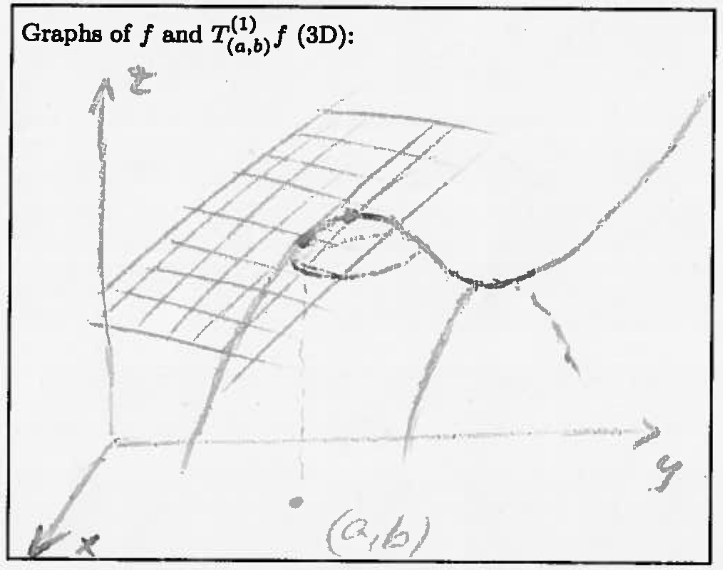
\includegraphics[width=0.6\textwidth]{./Figures/f306.png}
\end{center}
\end{enumerate}
\end{remark}

\begin{exercise}
\begin{enumerate}[(i)]
	\item Find the second-order Taylor approximation of $f(x,y)=x^2(1-y^3)$ at the point\footnote{
	\[ T_{(2,1)}^{(2)}f(x,y) = -12y^2-12xy+12x-36y-24 \]}
	$(a,b)=(2,1)$.
	\item Find the second-order Taylor approximation of $f(x,y,z)=xy^2+z^3$ at\footnote{You can verify your answer by checking the conditions in Remark~\ref{rem:taylor_appr}. To make sure that your second derivatives are correct, compare to the example at the end of the previous section.} $(a,b,c)=(1,1,1)$.
	\item Find the second-order Taylor approximation of $f(x,y)=\arctan(x+2y)$ at\footnote{
	\[ T_{(5,-2)}^{(2)}f(x,y) = -\frac{x^2}{4}-y^2-xy+x+2y+\frac{\pi-3}{4}\]}
	$(a,b)=(5,-2)$.
	\item Re-do example (ii) above, $f(x,y)=2x^2+y^2$, but now at a general point $(a,b)\in\mathbb{R}^2$. That is, use parameters $a$ and $b$ for the point at which the approximation is carried out, rather than specific numbers.
	\item Find the intersection of the $xy$-plane with the tangent plane of $f(x,y)=2x^2+y^2$ at\footnote{$y=x-\tfrac32.$} $(1,-2)$.
\end{enumerate}
\end{exercise}
	
	
\section{Local Extrema and Saddle Points}

\begin{definition}[Local Extrema and Critical Points]
For a function $f(x,y)$ and a point $(a,b)$ in its domain (similarly in three variables):
\begin{enumerate}[(i)]
	\item $(a,b)$ is a \emph{local maximum} of $f$ if 
	\[ f(x,y) \leq f(a,b) \]
	in some neighbourhood of $(a,b)$.
	\item $(a,b)$ is a \emph{local minimum} of $f$ if there exists an $\delta > 0$ such that
	\[ f(x,y) \geq f(a,b) \]
	for all $(x,y)$ with $\left|\left|\begin{bmatrix} x \\ y \end{bmatrix}
							   -\begin{bmatrix} a \\ b \end{bmatrix}\right|\right|<\delta$.
	\item $(a,b)$ is a \emph{critical point} of $f$ if 
	\[ \nabla f (a,b) = \begin{bmatrix} 0 & 0 \end{bmatrix} \:. \]
\end{enumerate}
\end{definition}

\begin{remark}
\begin{enumerate}[(i)]
	\item Neighbourhoods are small sets surrounding the point in question. For example, in one dimension: For $t_0 = 0.001$, there exists a small neighbourhood of $t_0$ that contains only positive numbers, e.g. the open interval $(t_0-0.0005,t_0+0.0005)$. For $t_0=0$, however, this is not possible: every neighbourhood -- no matter how small -- contains both positive and negative numbers. In the higher dimensional domains of multivariate functions, one can work with disks (in 2D) or balls (in 3D). This notion is very important in Mathematics and used informally in part (i) of the definition above. In part (ii), the same condition is written out more formally using a parameter $\delta$ and the corresponding disk of radius $\delta$ around the point $(a,b)$. It does not matter how small $\delta$ is, but $\delta>0$ is essential.
	\item A local extremum is either a local minimum or a local maximum. Local maxima are not surpassed in some small neighbourhood, while for local minima there exists a neighbourhood in which none of the other function values is smaller. There is no requirement for surrounding function values to be strictly smaller, respectively strictly larger -- that means, for example, that for a constant function $f(x,y)=c$, every point in its domain is both a local maximum and a local minimum.
	\item For the material in this section, it is useful to recall the corresponding single-variable theory. The following result should look familiar and its proof will be left as an exercise.
\end{enumerate}
\end{remark}

\begin{theorem}
\label{thm:crit_pts}
If $(a,b)$ is a local extremum of $f$, then $(a,b)$ is a critical point of~$f$.
\end{theorem}

\begin{example}
\label{expl:crit_points}
	\begin{enumerate}[(i)]
		\item Find the critical points of $f(x,y) = x^2y - y + 7$.\\
		{\it Sol.:}
		The gradient of $f$ is 
		\[  \nabla f (x,y) = \begin{bmatrix} 2xy & x^2-1 \end{bmatrix} \:. \]
		Setting its second component, i.e., the $y$-derivative of $f$, equal to zero, we obtain $x^2-1=0$, which has solutions $x=\pm1$. The second equation is $2xy=0$, which, since we know $x\not=0$, has the solution $y=0$. Therefore, the critical points are $(-1,0)$ and $(+1,0)$.
		\item Find the critical points of $f(x,y) = xy$.\\
		{\it Sol.:}
		Setting the gradient of $f$,
		\[  \nabla f (x,y) = \begin{bmatrix} y & x \end{bmatrix} \:, \]
		equal to zero gives the critical point $(a,b)=(0,0)$.
		
		Note, however, that this is not a local extremum: The function value at that point is $0$, and there are points with both positive and negative function values arbitrarily close to it. For example, consider the points $(x,y)=(\varepsilon,\varepsilon)$ and $(x,y)=(\varepsilon,-\varepsilon)$, where $\varepsilon$ is a small positive constant.
		\item Find the critical points of $f(x,y) = x^3 - 3x + 3xy^2$.\\
		{\it Sol.:}
		After computing the gradient of $f$, we find that $f_x=0$ for all points on the unit circle, and $f_y=0$ for all points that lie on one of the two axes. This gives the critical points $(+1,0)$, $(0,+1)$, $(-1,0)$, $(0,-1)$.
	\end{enumerate}
\end{example}

\begin{theorem}[Second-Derivative Test]
Let $(a,b)$ be a critical point of $f(x,y)$ and let 
\[ \Delta = \det \left( \mathrm{Hess} f (a,b) \right) 
= \left( f_{xx}f_{yy}-f_{xy}^2 \right)_{|(a,b)} \:. \]
Then $(a,b)$ can be classified as follows.
\begin{enumerate}[(i)]
	\item If $\Delta > 0$ and $f_{xx}(a,b)>0$, then $(a,b)$ is a local minimum.
	\item If $\Delta > 0$ and $f_{xx}(a,b)<0$, then $(a,b)$ is a local maximum.
	\item If $\Delta < 0$, then $(a,b)$ is not a local extremum.
	\item If $\Delta = 0$, then the test is inconclusive and $(a,b)$ could be any of the three possibilities above (local maximum, local minimum, or neither).
\end{enumerate}
\end{theorem}

\begin{example}
\label{expl:classifications}
\begin{enumerate}[(i)]
	\item Find and classify all critical points of $f(x,y) = x^2y - y + 7$.\\
	{\it Sol.:} In the previous example, we have found the critical points $P_1=(-1,0)$ and $P_2=(+1,0)$. The Hessian of $f$ is
	\[ \mathrm{Hess}f(x,y) =
	\begin{bmatrix}	2y & 2x \\ 2x & 0 \end{bmatrix} \:. \]
	At the first point, we have
	\[ \mathrm{Hess}f(P_1) =
	\begin{bmatrix}	0 & -2 \\ -2 & 0 \end{bmatrix} \:, \]
	which has determinant $\Delta = 0 \cdot 0 - (-2) \cdot (-2) = -4 < 0$. Hence, $P_1$ is neither a local maximum nor a local minimum. Points like $P_1$ are called \emph{saddle points}, cf. Remark~\ref{rem:schmiegquadriken}.
	At the second critical point, we have
	\[ \mathrm{Hess}f(P_2) =
	\begin{bmatrix}	0 & 2 \\ 2 & 0 \end{bmatrix} \:, \]
	which has determinant $\Delta = 0 \cdot 0 - 2 \cdot 2 = -4 < 0$. Hence, $P_2$ is a saddle point as well and therefore not a local extremum.
	\item Find and classify all critical points of $f(x,y) = x^3 - 3x + 3xy$.\\
	{\it Sol.:} Earlier we had found the critical points $P_1=(+1,0)$, $P_2=(0,+1)$, $P_3=(-1,0)$, and $P_4=(0,-1)$. The Hessian of $f$ is
	\[ \mathrm{Hess}f(x,y) =
	\begin{bmatrix}	6x & 6y \\ 6y & 6x \end{bmatrix} = 
	6\begin{bmatrix}	x & y \\ y & x \end{bmatrix} \:. \]
	This gives
	\[ \mathrm{Hess}f(P_1) = 6 I, \qquad \mathrm{Hess}f(P_3) = -6 I \:, \]
	which both have determinant $\Delta = +36 > 0$. Inspecting the signs of the entries in the upper left of those Hessians, we find that $P_1$ is a local minimum and that $P_3$ is a local maximum. At $P_2$ and $P_4$, we have
	\[ \mathrm{Hess}f(P_{2/4}) =
	\begin{bmatrix}	 0 & \pm6 \\ \pm6 & 0 \end{bmatrix} \:, \]
	which both have determinant $\Delta = -36 < 0$. Therefore, $P_2$ and $P_4$ are not local extrema.
	\item Find all critical points of 
	$f(x,y) = x - \ln x + 2 y^2 + xy$
	and classify them using the second derivative test.\\
	{\it Sol.:}
	\begin{equation*}
	\begin{split}
	f(x,y) &= x - \ln x + 2 y^2 + xy \:, \\
	\nabla f (x,y) & = \begin{bmatrix} 1 - \tfrac{1}{x} + y & 4y + x \end{bmatrix} \:,\\
	\mathrm{Hess}f(x,y) &= \begin{bmatrix} \rfrac{1}{x^2} & 1 \\ 1 & 4 \end{bmatrix} \:,\\
	P &= (2,-\tfrac{1}{2}) \:,\\
	\Delta &= 0 \:.
	\end{split}
	\end{equation*}
	Therefore, the second derivative test is inconclusive, and more work is required to classify the critical point $P=(2,-\tfrac{1}{2})$ of $f$.
\end{enumerate}
\end{example}

\begin{remark}
\label{rem:schmiegquadriken}
It is useful to understand the workings behind the second derivative test. We therefore sketch its derivation:

Since $(a,b)$ is a critical point of $f$, the second-order Taylor approximation	at that point is 
\[ T_{(a,b)}^{(2)} f (x,y) = f(a,b) + 0 
 + \frac{1}{2} \begin{bmatrix} x-a & y-b \end{bmatrix}
\mathrm{Hess} f (a,b) \begin{bmatrix} x-a \\ y-b \end{bmatrix} \:, \]
and it seems plausible that studying the approximation $T_{(a,b)}^{(2)}f$ should allow to classify $(a,b)$. Now, for the question whether $(a,b)$ is an extremum or not, overall additive constants such as the term $f(a,b)$ above do not matter. Also, we may shift our coordinate system so that $(a,b)\rightarrow(0,0)$. That is, we let $\wtd{x}=x-a$, $\wtd{y}=y-b$, as in the proof of the Taylor approximation, and we then write $\wtd{x}$ and $\wtd{y}$ as $x$ and $y$ again to simplify the notation. Thirdly, we denote the matrix $\tfrac12 \cdot \mathrm{Hess}f$ at the critical point by $M$. Note that $M$ is symmetric. With those steps, we have reduced classifying the critical point $(a,b)$ of the original function $f$ to classifying the critical point $(0,0)$ of the auxiliary function
\[ h(x,y) = \begin{bmatrix}	x & y \end{bmatrix} M 
\begin{bmatrix} x \\ y \end{bmatrix} \:. \]

More advanced theory of matrices implies that it suffices to restrict one's attention to the case when $M$ is a diagonal matrix. The basic idea for this argument is: if $M$ is not diagonal, then there is a change of variables so that $M$ written out in the new variables is diagonal. This change of variables is a rotation of the $xy$-plane, which does not affect the property of being a minimum, maximum, or neither. The function $h$ is now of the form
\[ h(x,y) = \begin{bmatrix}	x & y \end{bmatrix}  
\begin{bmatrix}	\lambda & 0 \\ 0 & \mu \end{bmatrix}
\begin{bmatrix} x \\ y \end{bmatrix} \:, \]
where $\lambda,\mu\in\mathbb{R}$. For example, consider the case $\lambda = 4$, $\mu = 1$. Then
\[ h(x,y) = 4 x^2 + y^2 = (2x)^2 + y^2 = \wtd{x}^2+y^2 \:, \]
where we rescaled the $x$ axis, $x \rightarrow \wtd{x} = 2x$. The expression on the right is a paraboloid, for which $(0,0)$ is a minimum. The rescaling causes a deformation -- imagine a paraboloid, then squeeze it so that its level sets are ellipses rather than circles -- but, again, this does not affect the property of having a minimum, maximum, or neither at the point $(0,0)$. We have therefore found that $h$ with $\lambda = 4$ and $\mu = 1$ has a local minimum at $(0,0)$. By this argument, we find that all the cases with $\lambda > 0$ and $\mu > 0$ are qualitatively the same and have a minimum. Let us choose the identity matrix as representing those cases,
\[ M_1 = I = \begin{bmatrix} 1 & 0 \\ 0 & 1 \end{bmatrix} \:, \]
for which $h(x,y)=x^2+y^2$ and the graph of $h$ is a paraboloid:
%\figbox{Example for case (i) ($h$ induced by $M_1$, paraboloid; 3D):}
\begin{center}
	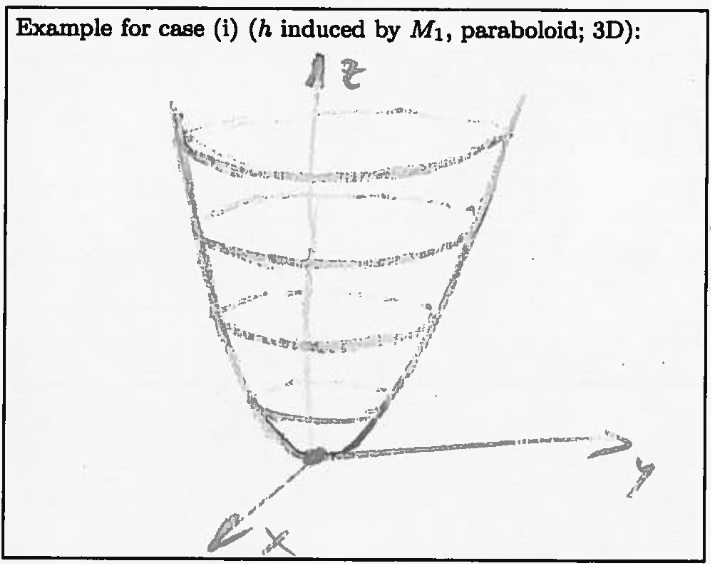
\includegraphics[width=0.6\textwidth]{./Figures/f307.png}
\end{center}
This is case (i) of the second derivative test, a local minimum. Note that the chosen representative $M_1=I$ for this class satisfies the assumptions of (i): $\det M_1 > 0$ and its upper left entry is positive.

Continuing this line of reasoning, one finds that the other cases to consider are:
\begin{equation*}
M_2 = \begin{bmatrix} -1 & 0 \\ 0 & -1 \end{bmatrix} \:,
M_3 = \begin{bmatrix} +1 & 0 \\ 0 & -1 \end{bmatrix} \:,
M_4 = \begin{bmatrix} +1 & 0 \\ 0 & 0 \end{bmatrix} \:, 
M_5 = \begin{bmatrix} -1 & 0 \\ 0 & 0 \end{bmatrix} \:, 
M_6 = \begin{bmatrix} 0 & 0 \\ 0 & 0 \end{bmatrix} \:.
\end{equation*}
The matrix $M_2$ generates the upside-down paraboloid $h(x,y)=-(x^2+y^2)$,
%\figbox{Example for case (ii) ($h$ induced by $M_2$, upside-down paraboloid; 3D):}
\begin{center}
	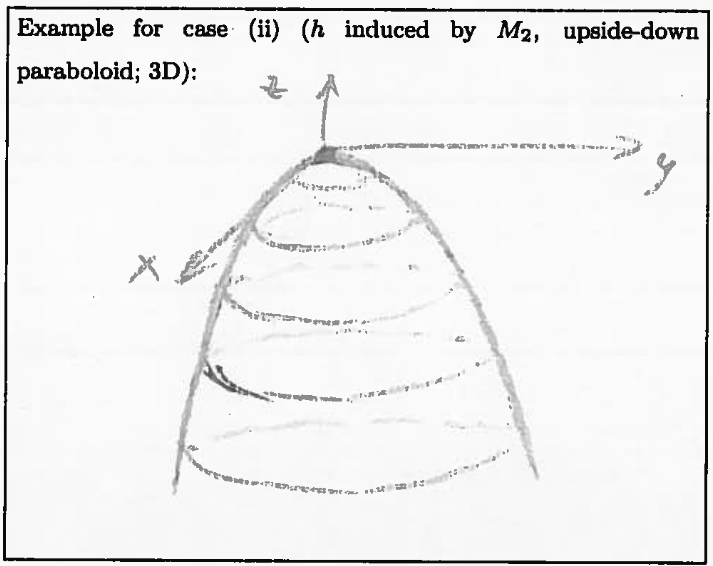
\includegraphics[width=0.6\textwidth]{./Figures/f308.png}
\end{center}
which has a maximum at $(0,0)$. Again, note that $M_2$ satisfies the assumptions of (ii) of the second derivative test. The matrix $M_3$ gives
\[ h(x,y) = x^2-y^2 \:, \]
which does not have an extremum at $(0,0)$: we have $h(0,0)=0$, but both positive and negative function values arbitrarily close (e.g. $h(\varepsilon,0)>0$ and $h(0,\varepsilon)<0$). This is case (iii) of the second derivative test, and both the graph of $h(x,y) = x^2-y^2$,
%\figbox{Example for case (iii), ($h$ induced by $M_3$, saddle; 3D):}
\begin{center}
	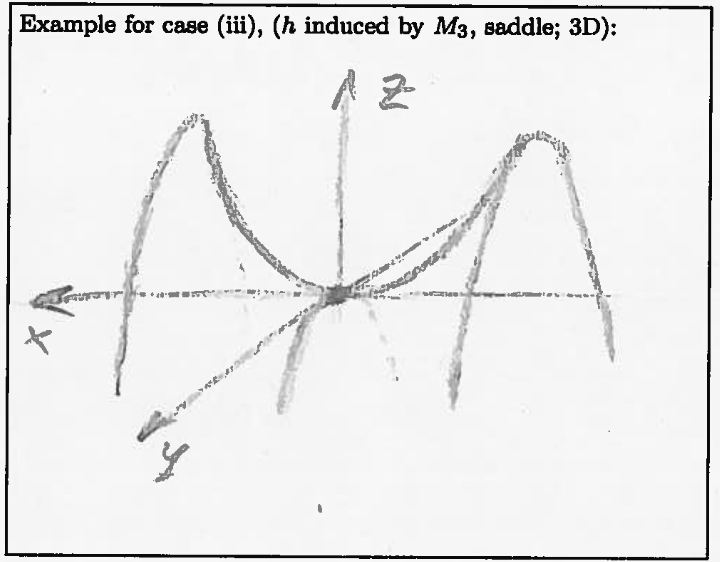
\includegraphics[width=0.6\textwidth]{./Figures/f309.png}
\end{center}
and the form of $M_3$ agree with the statements in (iii).

Finally, we argue that the cases represented by $M_4,M_5,M_6$ do not allow us to draw a conclusion, i.e. they correspond to case (iv) of the second derivative test. They all do satisfy the assumption $\det M = 0$. The choice $M_5$ gives $h(x,y)=-x^2$, which has the following graph.
%\figbox{Example for case (iv) ($h$ induced by $M_5$; 3D):}
\begin{center}
	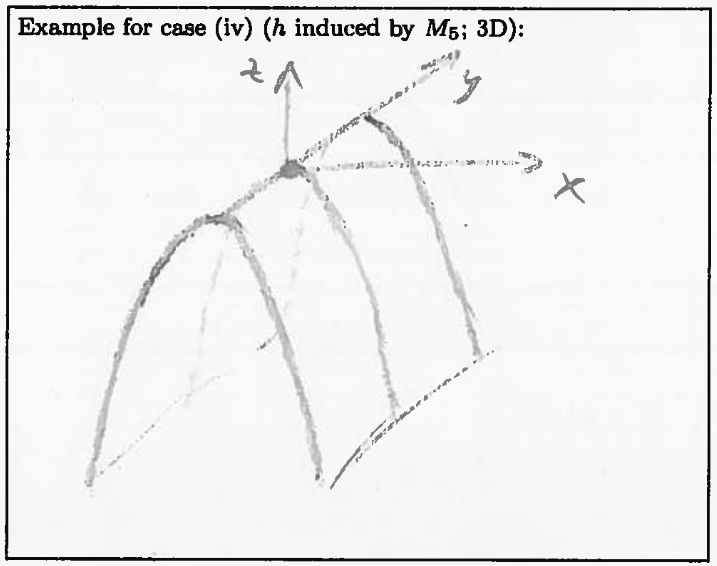
\includegraphics[width=0.6\textwidth]{./Figures/f310.png}
\end{center}
The matrix $M_4$ produces the same graph, but upside-down, and the graph obtained by choosing $M_6$ is the plane $h(x,y)=0$. In each of these cases, there is at least one straight line passing through the critical point $(0,0)$ in question. On this line, small contributions of the original function $f$, that are not captured by the second-order Taylor approximation, could tip the balance to different conclusions. Some guidance for understanding this will be provided in the exercises below.

The purpose of this remark was to explain the workings behind the second derivative test, to outline its proof, and, perhaps most importantly, to help avoid confusion of the cases (i) and (ii): For example, suppose you are classifying a critical point, you have obtained a Hessian matrix with positive determinant and positive entry in the upper left corner, but you have forgotten whether this implies a minimum or a maximum. Then think of the representative $M = I$ of this situation -- this gives the function $h(x,y) = x^2 + y^2$, which is the well-known paraboloid, which has a \emph{minimum} at $(0,0)$.
\end{remark}

\begin{application}[Mean squared error for linear regression]
\texttt{Define mean squared error for the linear regression application from the previous chapter; apply theory from the current chapter to basic matrix functions and hence show that linear regression minimises the MSE.}
\end{application}

\begin{exercise}
	\begin{enumerate}[(i)]
		\item Fill in the gaps for examples \ref{expl:crit_points} (iii) and \ref{expl:classifications} (iii), which were only sketched.
		\item Find an classify all critical points of\footnote{Only one critical point: a saddle point at $(-2,4)$.}
		$f(x,y) = x^2+xy+2y-1$. 
		\item Find and classify all critical points of\footnote{The critical points are
		\[ (0,0)\:,\quad(2,0)\:,\quad(1,1)\:,\quad(1,-1), \]
		and they are a maximum, minimum, saddle point, saddle point, respectively.}
		$f(x,y) = x^3+3xy^2-3x^2-3y^2-2$.
		\item Convince yourself that Theorem~\ref{thm:crit_pts} is true\footnote{You could contrapose that statement and/or look at Theorem~\ref{thm:geom_dd} for inspiration.}.
		\item Give examples of a local minimum, a local maximum, and a critical point that is neither, that cannot be classified with the second derivative test\footnote{$f(x,y)=x^4+y^4$ covers one of those cases.}.
	 	\item Use graphing software to explore different functions of the form
	 	\[ h(x,y) = \begin{bmatrix} x & y \end{bmatrix}
	 	M \begin{bmatrix} x \\ y \end{bmatrix} \:, \]
	 	where $M$ is a symmetric $2 \times 2$ matrix (i.e., $a_{12}=a_{21}$), and compare the different shapes you find to Remark~\ref{rem:schmiegquadriken}.
	 	\item For \ref{expl:classifications} (iii), use graphing software to find out what the point $P$ is\footnote{Classifying $P$ is quite difficult. Zooming in by appending \texttt{~for x from 1.99 to 2.01 and y from -0.51 to -0.49~} to the WolframAlpha plot command provides some insight.}.
	\end{enumerate}
\end{exercise}


\section{Extrema under Constraints: Lagrange Multipliers}

\begin{example}
\label{expl:naive_opt}
Find the maximum of the function $z=f(x,y)=2x+y$ on the circle $S = \{ (x,y) \in \mathbb{R}^2 \: | \: x^2+y^2=1 \}$, as well as the value that $f$ takes at that point.\\
{\it Sol.:} First note that the graph of $f$ is a plane, and therefore $f$ does not have any extrema at all on its full domain $\mathbb{R}^2$. However, a maximum does exist when restricting to the circle:
%\figbox{Maximum of $f$ on $S$ (3D):}
\begin{center}
	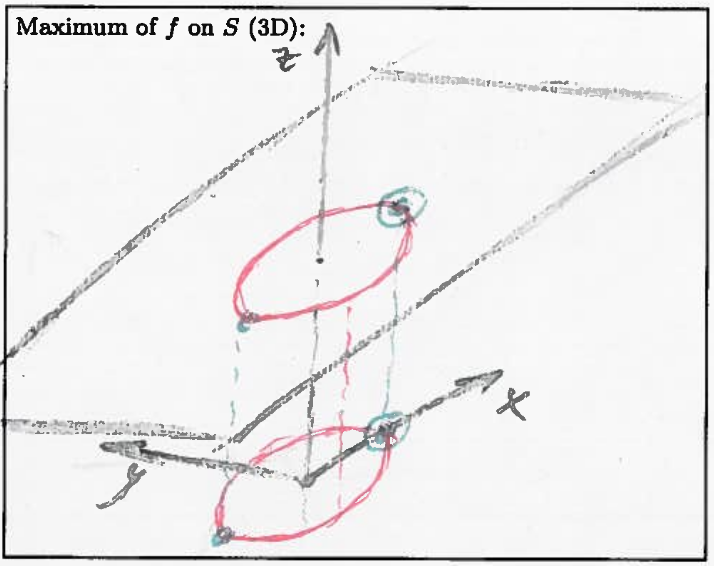
\includegraphics[width=0.6\textwidth]{./Figures/f311.png}
\end{center}
To find this point, we parametrise the circle as
\[ (x(t),y(t)) = (\cos(t),\sin(t)) \:, \]
and then define the function $F(t)=f(x(t),y(t))$. This gives
\begin{equation*}
\begin{split}
F(t) &= 2\cos(t)+\sin(t) \:, \\
F'(t) &= -2\sin(t)+\cos(t) \:.
\end{split}
\end{equation*}
Setting $F'(t)$ equal to zero, we obtain
\[ \tan(t_0) = \frac12 \:, \]
which has solutions $t_0 \approx 0.464 + k\pi$. Taking $k=0$ and $k=1$ leads to the points
\begin{equation*}
\begin{split}
(x_1,y_1)&\approx(\cos(0.464),\sin(0.464))\approx(0.894,0.448) \:, \\
(x_2,y_2)&\approx(\cos(3.606),\sin(3.606))\approx(-0.894,-0.448) \:,
\end{split}
\end{equation*}
and all other $k$ will yield one of those two points again. Evaluating, we see that $f$ has a larger value at $(x_1,y_1)$, and hence we obtain the answer: $f$ takes the maximum value $2.236$ on the circle $S$ at the point $(x,y)=(0.894,0.448)$.
\end{example}

\begin{remark}
Now suppose the set $S$ is given as a level set of a function $g$, and is less regular and can not be parametrised easily. The following figure shows such a set $S$ in the domain of $f$, and further a level set $f(x,y)=c$, where the constant $c=c_1$ is chosen to be larger than any of the values $f$ takes on $S$.
%\figbox{The level sets $g=0$ and $f=c$ for large $c$ (2D):}
\begin{center}
	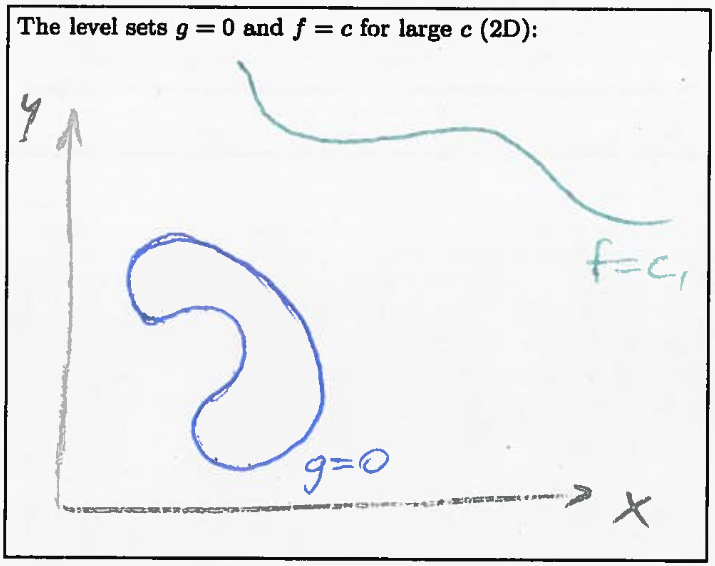
\includegraphics[width=0.6\textwidth]{./Figures/f312.png}
\end{center}
Now, choosing a slightly smaller constant $c_2$, the curve $f=c$ will move towards $g=0$. We continue this process until the first contact between the two curves is made, say for $c=c_3$. This contact point is a local maximum -- convince yourself of that\footnote{Can any of the other points in $S$ have larger function values?}!
%\figbox{The level sets $g=0$ and $f=c$ for smaller values of $c$ (2D):}
\begin{center}
	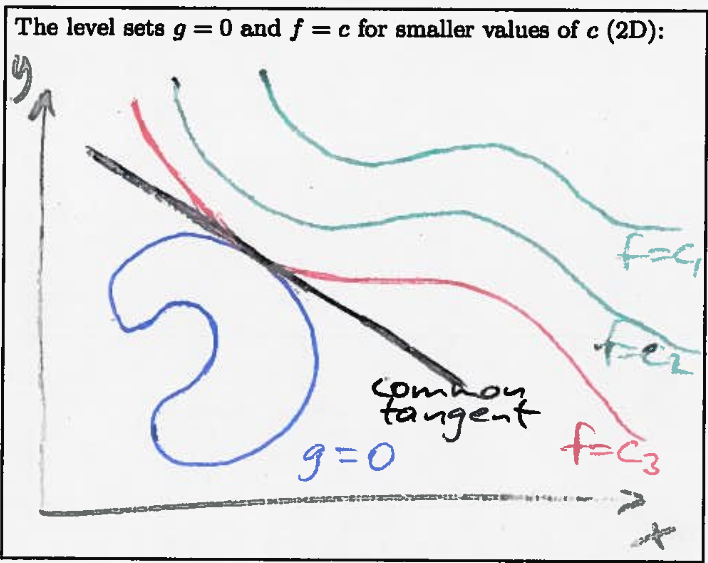
\includegraphics[width=0.6\textwidth]{./Figures/f313.png}
\end{center}
Note that the level curves $g=0$ and $f=c_3$ have a common tangent line -- convince yourself that this is always the case\footnote{Try to sketch a \emph{first-contact} scenario where the tangent lines at the contact point intersect (you will not succeed; be aware that level curves of smooth functions do not have ends -- they are either closed curves or they go out to infinity).}. Recall that gradient vectors are orthogonal to level sets and their tangent lines or planes. It must therefore be the case that the gradients of $f$ and $g$ are parallel:
\[ \nabla f = \lambda \nabla g, \qquad \text{for some~} \lambda \in \mathbb{R} \:. \]
\end{remark}

\begin{theorem}[Lagrange Multipliers]
To maximise or minimise a function $f(x,y)$ on a set 
$S = \{ (x,y) \in \mathbb{R}^2 \: | \: g(x,y) = 0 \} $,
define the function
\[ F(\lambda,x,y) = f(x,y) - \lambda g(x,y) \:, \]
and then solve
\[ \nabla F = \begin{bmatrix} 0 & 0 & 0 \end{bmatrix} \:. \]
The function $f$ can then be evaluated at the solutions $(x,y)$ of that system to identify the extreme value. The parameter $\lambda$ is called \emph{Lagrange multiplier}.
\end{theorem}

\begin{example}
\label{expl:opt}
\begin{enumerate}[(i)]
	\item Re-do example \ref{expl:naive_opt} using Lagrange multipliers.\\
	{\it Sol.:} We have $f(x,y) = 2x + y$ and we let
	\[ g(x,y) = x^2 + y^2 - 1 \:, \]
	so that
	\[  S = \{ g=0 \} \:. \]
	Then we define
	\[ F(\lambda,x,y) = f(x,y) - \lambda g(x,y) = 2x+y - \lambda (x^2+y^2-1) \:, \]
	which has partial derivatives
	\begin{equation*}
	\label{eq:lagrange_system}
	\begin{split}
	F_\lambda(\lambda,x,y) & = 1-(x^2+y^2) \:, \\
	F_x(\lambda,x,y) & = 2 - 2\lambda x \:, \\
	F_y(\lambda,x,y) & = 1 - 2\lambda y \:.
	\end{split}
	\end{equation*}
	Setting $\nabla F$ equal to $0$ leads to a system of three equations (the equations are not linear, and hence the techniques from chapter~\ref{ch:vm} can not be used to solve it). The equations $F_x=0$ and $F_y=0$ lead to
	\[ x = \frac{1}{\lambda}, \qquad y = \frac{1}{2\lambda} \:, \]
	which we can then substitute into $F_\lambda=0$:
	\[ 0 = 1 - \left( \left( \frac{1}{\lambda} \right)^2 
	+ \left( \frac{1}{2\lambda} \right)^2 \right) 
	= 1 -\frac{5}{4\lambda^2} \quad \rightarrow \quad \lambda = \pm \frac{\sqrt{5}}{2} \:. \]
	Using the equations for $x$ and $y$ above, we obtain the points 
	\begin{equation*}
	\begin{split}
(x_1,y_1) &= \left( \frac{2}{\sqrt{5}},\frac{1}{\sqrt{5}} \right) \approx (0.894,0.447) \:, \\
(x_2,y_2) &= \left( -\frac{2}{\sqrt{5}},-\frac{1}{\sqrt{5}} \right) \approx (-0.894,-0.447) \:.
	\end{split}
	\end{equation*}
	Now, $f$ has to have both a maximum and a minimum on $S$ -- this is similar to the extreme value theorem for continuous single-variable functions -- and the two points above are the only candidates for those extrema. Evaluating, we find
	\[ f(x_1,y_1) = 2 \frac{2}{\sqrt{5}} + \frac{1}{\sqrt{5}} = \sqrt{5} \]
	and $f(x_2,y_2)= - \sqrt{5}$. Hence, $(x_1,y_1)$ is the maximum.
	
	Note that, contrary to the computation in example \ref{expl:naive_opt}, we did not have to numerically evaluate inverse trigonometric functions, and we were able to obtain exact symbolic expressions for the maximum function value and the coordinates of the point where it is taken. Also, comparing the two different approaches, we have proven that
	\[ \cos \left( \arctan \left( \frac{1}{2}\right)\right) = \frac{2}{\sqrt{5}} \:. \]
	\item Find the point on the surface $(x-y)^2-z^2 = 1$ that is closest to the origin $(x,y,z)=(0,0,0)$ of $\mathbb{R}^3$.\\
	{\it Sol.:}
	The function
	\[ d(x,y,z) = \sqrt{x^2+y^2+z^2} \:, \]
	which assigns to every point in $\mathrm{R}^3$ its distance from the origin, needs to be minimised on the surface
	\[ S = \{ x,y,z\in \mathbb{R} \: | \: (x-y)^2-z^2 = 1\} \subseteq \mathbb{R}^3 \:. \]
	Suppose we have found a point $P \in S$ with minimal $d(P)$. Then $(d(P))^2$ will be minimal as well (the formal justification for this step is that $x \mapsto x^2$ is monotonously increasing for $x \geq 0$). Hence we can simplify our computations by minimising 
	\[ f(x,y,z) = x^2+y^2+z^2 \]
	instead of $d$. The function $g(x,y,z)=(x-y)^2-z^2-1$ defines $S$ and gives
	\[ F(\lambda,x,y,z) = x^2+y^2+z^2-\lambda((x-y)^2-z^2-1) \:. \]
	Setting the gradient of $F$ equal to zero, we obtain the system
	\begin{equation*}
		\begin{cases}
			0 &= 2x - \lambda \cdot 2(x-y) \:, \\
			0 &= 2y - \lambda \cdot 2(x-y)(-1) \:, \\
			0 &= 2z - \lambda \cdot (-2z) \:, \\
			0 &= 1+z^2-(x-y)^2 \:.
		\end{cases}
	\end{equation*}
	There are different ways to solve this, and it is important to gain experience with computations of that kind in order to be able to carry them out efficiently and with confidence. Combining the first two equations yields $y=-x$ and the new system
	\begin{equation*}
		\begin{cases}
			0 &= 2x (1 - 2 \lambda) \:, \\
			0 &= 2z (1 + \lambda) \:, \\
			0 &= 1 + z^2 - 4x^2 \:.
		\end{cases}
	\end{equation*}
	In R1, one of the two factors has to be $0$. Taking $x=0$, R3 becomes $1+z^2=0$, which does not have solutions. Taking $\lambda=\tfrac{1}{2}$ in R1 leads to the points
	\[ P_{1/2} \: : \: (x,y,z) = \left( \pm\frac12, \mp\frac12,0 \right) \:. \]
	The function values at those critical points are $f(P_1)=f(P_2)=\tfrac12$, corresponding to distances $d(P_1)=d(P_2)=\tfrac{\sqrt{2}}{2}$ from the origin. Now, there have to be points of minimal distance to the origin on $S$, and since the two critical points we have found are the only candidates for such extrema, we see that $P_1$ and $P_2$ are minima. Note that $f$ does not have any maxima -- this is possible because $S$ is unbounded.
	\item Bob wants to sell free-range eggs and needs to decide how many chicken to keep (``$x$'') and how much land to lease (``$y$''). In order to be able to label his eggs as free-range, every chicken needs to have at least $4\,m^2$ of space. Leasing land costs $f_2(y)=\rfrac{y}{10}$ and selling eggs brings in an income $f_1(x)=8\sqrt{x}$. Help Bob optimise his profits. (The numbers in this problem are fictional.)\\
	{\it Sol.:}
	\begin{equation*}
	\begin{split}
	 \mathrm{Profit}\: &: \quad f(x,y) = f_1(x) - f_2(y) \:, \\
	 \mathrm{Function~}F\: &: \quad
	 F(\lambda,x,y) = 8\sqrt{x} - \frac{y}{10} - \lambda \left( \frac{y}{x}-4 \right) \:, \\
	 \mathrm{Answer}\: &: \quad x=100, \quad y=400, \quad f_{\text{max}} = 40 \:.
	\end{split}
	\end{equation*}
\end{enumerate}	
\end{example}

\begin{exercise}
\begin{enumerate}[(i)]
	\item Find the maximum of $f(x,y)=x$ on\footnote{Maximising that function amounts to finding the point of the curve that has the largest $x$-coordinate: $x_{\text{max}}=1$, taken at $(x,y)=(1,0)$.} $x^3+y^2=1$.
	\item Just to make sure we are not sending Bob down the wrong path: also solve example~\ref{expl:opt} (iii)  with single-variable theory, as in example~\ref{expl:naive_opt}.
	\item Find the maximum and minimum value of $f(x,y)=x^3y^5$ on the ellipse\footnote{The maximum and minimum values of $f$ are $\pm5^{\rfrac52}$, taken at the points $(\pm1,\pm\sqrt{5})$.} $3x^2+y^2=8.$
	\item Find the point on $S\,:\:z= xy$ that is closest to the sphere of radius $1$ centred at\footnote{A point on $S$, that is closest to the sphere, is also closest to its centre; considering different cases helps solving $\nabla F = 0$; to check your answer: you should obtain a minimum distance of $2$.} $(x,y,z)=(0,0,5)$.
	\item A single-variable problem similar to example \ref{expl:opt} (ii): For $c\in\{1,-4\}$, consider the curve $y=x^2+c$ and the distances of its points to the origin $(0,0)$ of the $xy$-plane. Sketch the curves and think about what kind of extrema exist in each case. Then compute all local and global extrema as well as the corresponding distances to the origin\footnote{You should obtain four extrema with distances $1$, $1.936$, and $4$ to the origin. The minima are both local and global, the maximum is only local. Make sure to state the extrema (the points at which the minimal/maximal distances are realised), as they are part of what you were asked for.}.
	\item Find the maximum value of 
	\[ f(x,y,z) = \ln x + \ln y + 3 \ln z \:, \quad x>0,y>0,z>0 \]
	on the sphere $x^2+y^2+z^2 = 5R^2$.
\end{enumerate}	
\end{exercise}

\chapter{Integration \texttt{(written; to be expanded and brushed up)}}
\label{ch:i}
\begin{center}
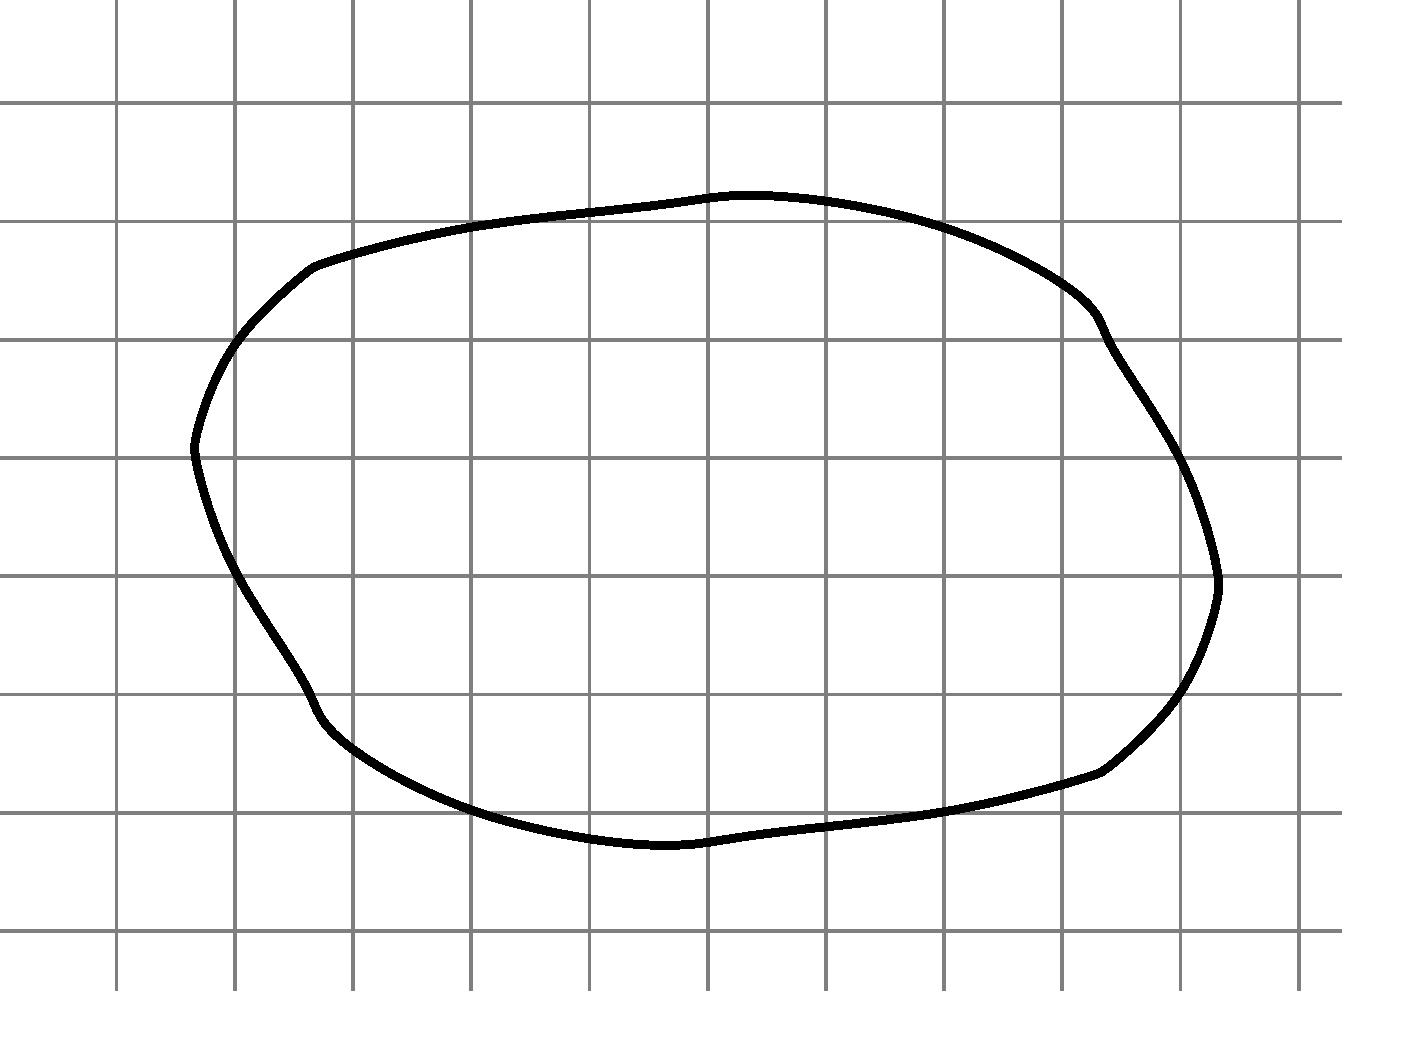
\includegraphics[width=0.6\textwidth]{./Figures/tiled_room.pdf}
\end{center}

Suppose you have an oddly shaped room with square tiles, and you want to estimate its square footage. Let $n$ be the number of full tiles you count, and let $m$ stand for the number of broken tiles. Denote the area of a single tile -- which can be computed: it is the square of the side length -- by $A_0$. Then we have the lower and upper bounds
\[n \cdot A_0 \leq A \leq (n+m) \cdot A_0\]
for the area $A$ of the room. Now, convince yourself that this estimate would be better (tighter), if the tiles were smaller\footnote{Mark the areas $n \cdot A_0$ and $(n+m) \cdot A_0$ in the sketch above, and then think about what would happen if we had tiles of half the side length}!

Finding areas under curves or volumes under surfaces is called \emph{integration}. It is one of the most fundamental and important concepts of mathematics, and it has applications in every scientific discipline. The above approach of approximating areas with large numbers of simple pieces can be quite cumbersome. Fortunately, there is very powerful connection to differentiation, which allows to compute integrals in a more efficient way.

\begin{application}[Centre of mass]
A large metal plate of uniform thickness and the shape in the sketch (let us call it $S$; the area under $f(x)=\sqrt{x}$ for $x$ from $0$ to $9$) needs to be balanced on a single point.
\begin{center}
	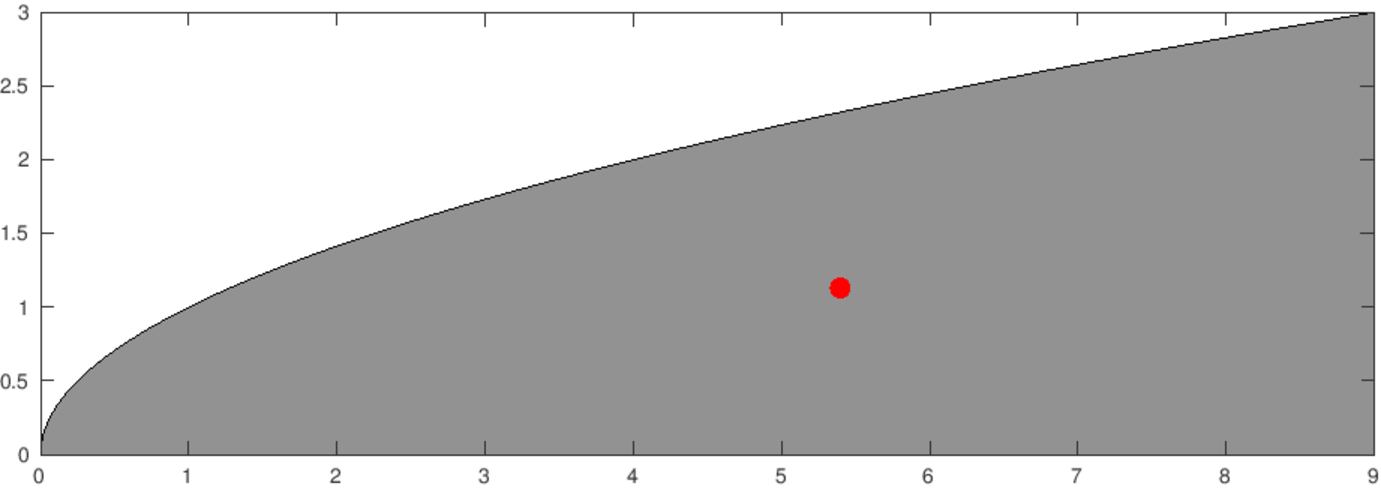
\includegraphics[width=0.6\textwidth]{./Figures/centre_of_mass.pdf}
\end{center}
That is, the centre of mass of $S$ needs to be found.

This can be solved with integration: The $x$ and $y$ coordinates of the centre of mass of $S$ are
\begin{align*}
x_c &= \frac{\iint_S x \: \d A}{\iint_S 1 \: \d A} = 5.4, \\
y_c &= \frac{\iint_S y \: \d A}{\iint_S 1 \: \d A} = 1.125.
\end{align*}
We will learn how to compute those integrals in this chapter.
\end{application}


\section{Theory of Integration in One Dimension}

\begin{definition}[Definite Integral, Riemann Sum]
Let $f(x)$ be continuous on $a \le x \le b$ and divide the interval
$[a,b]$ into $n$ subintervals of equal width $\Delta x = \rfrac{(b-a)}{n}$. Let
\[ x_0 = a, \:\: x_1 = a + \Delta x, \:\: x_2 = x_1 + \Delta x = x_0 + 2 \Delta x, \:\:
\dots, \:\: x_n = x_0 + n \Delta x = b \]
be the endpoints of these subintervals. 
\begin{enumerate}[(i)]
\item
Then the \emph{definite integral} of $f$ from $a$ to $b$ is defined as
\begin{equation}
\label{eq:def_itgr}
\itgr{a}{b}{f(x)}{x} := \lim_{n \to \infty} \sum_{j=1}^{n} f(c_j) \Delta x,
\end{equation}
where $x_{j-1} \le c_j \le x_{j}$. Here $f(x)$ is called the \emph{integrand}, $a$ the lower boundary, and $b$ the upper boundary.
\item
The sum appearing in the above definition is called a \emph{Riemann sum} of $f$ over $[a,b]$. If the points $c_j$ are always chosen to be the right-hand end point of their subinterval, that is $c_j=x_j$, we obtain the right-hand Riemann sum
\[ \sum_{j=1}^{n} f(x_j) \Delta x. \]
Using the left end points of the subintervals, $c_j=x_{j-1}$, gives the left-hand Riemann sum
\[ \sum_{j=1}^{n} f(x_{j-1}) \Delta x = \sum_{j=0}^{n-1} f(x_{j}) \Delta x. \]
\end{enumerate}	
\end{definition}

\begin{remark}
\label{rem:def_int}
\begin{enumerate}[(i)]
	\item Equation~\eqref{eq:def_itgr} introduces a new quantity -- the definite integral of $f$ over $[a,b]$ -- and \emph{defines} (that is what the ``$:=$'' means) it to be equal to the limit for $n \rightarrow \infty$ of the Riemann sums on the right. Note that on the right-hand side of \eqref{eq:def_itgr}, different choices could be made for the points $c_j$. One should therefore show now that all these possible different choices lead to the same limit. That is, one should show that $\itgr{a}{b}{f(x)}{x}$ as defined above is \emph{well-defined}! This will be given as an exercise at the end of this section.
	\item The following figure illustrates the right-hand Riemann sum for $n=4$, 
	\[ \sum_{j=1}^{4} f(x_j) \Delta x, \]
	of some function $f$.
	\figbox{Right-hand Riemann sum of $f$ for $n=4$:}
	The rectangles in this figure have areas ``height'' $\cdot$ ``width'' 
	$= f(x_j)\cdot \Delta x$, and they are added up to obtain the Riemann sum. For comparison, the left-hand Riemann sum is
	\figbox{Left-hand Riemann sum of $f$ for $n=4$:}
	We see that in both cases, the Riemann sums approximate the area under the curve $y=f(x)$, and as in the example of the oddly-shaped room in the introduction, those approximations will get better if we choose $n$ to be larger. We can therefore interpret their limit, i.e., $\itgr{a}{b}{f(x)}{x}$, as the signed area under the curve $y=f(x)$:
	\figbox{Definite integral of $f$ over the integral $[a,b]$:}
	Here, the word ``signed'' was added since areas below the $x$-axis contribute negatively to the definite integral.
\end{enumerate}
\end{remark}

\begin{example}
Consider $f(x)=	\rfrac35 \, x$, $a=0$, $b=5$. First, let us find the left-hand Riemann sum for $n=5$ of $f$. The partition of $[a,b]=[0,5]$ is
\begin{equation*}
\begin{split}
\Delta x &= \frac{b-a}{n} = \frac{5-0}{5} = 1,\\
x_0 &= 0, \: x_1 = 1, \: x_2 = 2, \: \dots, x_5 = 5,
\end{split}
\end{equation*}
and therefore
\begin{equation*}
\begin{split}
\itgr{0}{5}{\frac{3}{5} \, x}{x} & \approx \sum_{j=0}^4 f(x_j) \Delta x 
= [f(0)+f(1)+f(2)+f(3)+f(4)] \cdot 1 \\
& = \frac35 \, [0+1+2+3+4] = 6.
\end{split}
\end{equation*}
We now generalise this computation to find the definite integral $f$ over the interval $[a,b]$.
The partition of the interval is
\begin{equation*}
\begin{split}
\Delta x &= \frac{b-a}{n} = \frac{5-0}{n} = \frac{5}{n},\\
x_0 &= 0, \: x_1 = \frac{5}{n}, \: x_2 = 2\frac{5}{n}, \: \dots, x_n = n\frac{5}{n}=5,
\end{split}
\end{equation*}
and therefore
\begin{equation*}
\begin{split}
\itgr{0}{5}{\frac{3}{5} \, x}{x} & = \lim_{n \to \infty} \sum_{j=0}^{n-1} f(x_j) \Delta x 
= \lim_{n \to \infty} \frac{5}{n} \sum_{j=0}^{n-1} \frac{3}{5} x_j  \\
& = \lim_{n \to \infty} \frac{5}{n} \sum_{j=0}^{n-1} \frac{3}{5} \frac{5}{n} \, j
= \lim_{n \to \infty} \frac{15}{n^2} \sum_{j=0}^{n-1} j \\
& = \lim_{n \to \infty} \frac{15}{n^2} \frac{(n-1)n}{2}
= \lim_{n \to \infty} \frac{15}{2} \frac{n-1}{n} = 7.5,
\end{split}
\end{equation*}
Note that this result agrees with the area
\[ A = \frac{3\cdot5}{2}, \]
found by noticing that the region under the curve $y=f(x)$ is a right-angled triangle.
\end{example}

\begin{properties}
\label{prop:di}
Let $a,b,\alpha\in\mathbb{R}$, $a<b$, and let $f(x),g(x)$ be continuous functions on $[a,b]$. Then:
\begin{equation*}
\begin{split}
(1) \qquad & \itgr{a}{a}{f(x)}{x} = 0, \\
(2) \qquad & \itgr{a}{b}{f(x)}{x} = -\itgr{b}{a}{f(x)}{x}, \\
(3) \qquad & \itgr{a}{b}{[f(x)+g(x)]}{x} = \itgr{a}{b}{f(x)}{x} + \itgr{a}{b}{g(x)}{x}, \\
(4) \qquad & \itgr{a}{b}{\alpha \cdot f(x)}{x} = \alpha \cdot \itgr{a}{b}{f(x)}{x}, \\
(5) \qquad & \itgr{a}{b}{f(x)}{x} = \itgr{a}{c}{f(x)}{x} + \itgr{c}{b}{f(x)}{x}  \\
(6) \qquad & \text{If~} f(x) \ge 0 \text{~on~} [a,b] \text{,~then} \itgr{a}{b}{f(x)}{x} \ge 0.
\end{split}
\end{equation*}
Now suppose that $f(x)$ is continuous on the interval $[-a,a]$, where $a>0$. Then we have
\begin{equation*}
\begin{split}
(7) \qquad & \text{If $f(x)$ is even, i.e. $f(-x)=f(x)$, then} 
	\itgr{-a}{a}{f(x)}{x} = 2\itgr{0}{a}{f(x)}{x}, \\
(8) \qquad & \text{If $f(x)$ is odd, i.e. $f(-x)=-f(x)$, then} \itgr{-a}{a}{f(x)}{x} = 0.
\end{split}
\end{equation*}
\end{properties}

\begin{remark}
\begin{enumerate}[(i)]
	\item All those properties are proven starting from the definition~\ref{eq:def_itgr} of the definite integral. (There is nothing else to start from, is there?) Only the proof of the last property is written out below.
	\item Properties (3) and (4) state that integration is \emph{linear}, and they can by proven by using the corresponding laws for sums and limits (e.g., pull the constant $\alpha$ out of the sum and then out of the limit in definition~\ref{eq:def_itgr}).
\end{enumerate}	
\end{remark}

\begin{proof}
For the proof of (8), we consider an odd function and we use only even $n$ for the limit $n\to\infty$. Since all choices for the points $c_j$ lead to the same limit, we make a choice that suits our purpose well: let the $c_j$ be the midpoints of their subintervals. The Riemann sums are
\[ \sum_{j=1}^n f(c_j) \Delta x 
= \Delta x \cdot \left[ f(c_1) + f(c_2) + \dots f(c_{n-1}) + f(c_n) \right], \]
and comparing to 
\figbox{An odd function and its Riemann sum, using midpoints:}
we see that this Riemann sum is zero since $f(c_1)+f(c_n)=0$, $f(c_2)+f(c_{n-1})=0$, \ldots This gives 
\[ \itgr{-a}{a}{f(x)}{x} = \lim_{n \to \infty} 0 = 0.\]

Now, the above assertion that $f(c_{j})+f(c_{n-j+1})=0$ seems to be confirmed by the sketch, but we should prove it properly: After working out formulas for the partition points $x_j$, we find
\[ c_j = -a+\Delta x\left(j-\frac12\right) = -a+\frac{2a}{n}\left(j-\frac12\right) \]
for the midpoints $c_j$ of the subintervals. This gives
\begin{equation*}
\begin{split}
c_{n-j+1} & = -a+\frac{2a}{n}\left(n-j+1-\frac12\right) \\
& = -a+2a+\frac{2a}{n}\left(-j+\frac12\right) = -c_j,
\end{split}
\end{equation*}
and therefore, since $f$ is odd,
\[ f(c_j)+f(c_{n-j+1})=f(c_j)+f(-c_j)=f(c_j)-f(c_j) = 0. \]
\end{proof}

\begin{definition}[Mean]
For continuous $f:[a,b]\rightarrow\mathbb{R}$, the real number
\[ \bar{f}:= \frac{1}{b-a} \itgr{a}{b}{f(x)}{x} \]
is called the \emph{mean} or \emph{average} of $f$ over the interval $[a,b]$.
\end{definition}

\begin{remark}
We have
\[ \bar{f}\cdot(b-a) = \itgr{a}{b}{f(x)}{x}, \]
that is, the area under the constant function $\bar{f}$ over $[a,b]$ is the same as the area under the graph of $f$:
\figbox{Definite integrals of $f$ and of the constant function $\bar{f}$:}
Note that this is similar for the average of numbers -- if Alice has an average of $\bar{m}$ on all the tests in a module, and Bob scored exactly $\bar{m}$ each time, then they have the same total mark.
\end{remark}

\begin{theorem}[Mean Value Theorem (MVT)]
Let $f:[a,b]\rightarrow\mathbb{R}$ be continuous. Then there exists a point $c\in(a,b)$ such that
\[ f(c) = \frac{1}{b-a} \itgr{a}{b}{f(x)}{x}. \]
That is, $f$ attains its mean value at some point in $(a,b)$.
\end{theorem}

\begin{proof}
Let
\[ M:=\max_{x\in[a,b]} f(x), \qquad m:=\min_{x\in[a,b]} f(x).\]
Since $f$ is continuous, it takes every value between $m$ and $M$. Therefore, we need to show that
\begin{equation}
\label{eq:proof_mvt}
 m \le \bar{f} \le M.
\end{equation}
We have
\begin{equation*}
\begin{split}
& M-f(x) \ge 0 \qquad \text{on~} [a,b] \\
\stackrel{\text{prop. (6)}}{\Longrightarrow} \quad & \itgr{a}{b}{M-f(x)}{x} \ge 0 \\
\stackrel{\text{prop. (3)}}{\Longrightarrow} \quad & \itgr{a}{b}{M}{x}-\itgr{a}{b}{f(x)}{x} \ge 0 \\
\Longrightarrow \quad & \itgr{a}{b}{f(x)}{x} \le \itgr{a}{b}{M}{x} = M(b-a).
\end{split}
\end{equation*}
Combining this with the outcome of the analogous computation for $f(x)-m$ gives
\[ m(b-a) \le \itgr{a}{b}{f(x)}{x} \le M(b-a). \]
Division by $(b-a)$ gives the inequality~\ref{eq:proof_mvt}, and hence completes the proof.
\end{proof}

\begin{definition}[Area Function]
For continuous $f:[a,b]\rightarrow\mathbb{R}$, the \emph{area function}
\[ A : [a,b] \rightarrow \mathbb{R} \]
of $f$ is
\[ A(x):=\itgr{a}{x}{f(t)}{t}. \]
\end{definition}

\begin{remark}
We use the variable $t$ in the integrand to avoid confusion with the variable of $A$.
\figbox{The area function for a continuous function $f$:}
\end{remark}

\begin{theorem}[Fundamental Theorem of Calculus (FTC)]
Let $f:[a,b]\rightarrow\mathbb{R}$ be continuous.
\begin{enumerate}[(i)]
	\item The derivative of the area function is
	\[ A'(x) = \Df{}{x} A(x) = f(x).\]
	That is,
	\[ \Df{}{x} \itgr{a}{x}{f(t)}{t} = f(x). \]
	\item If $F$ is any \emph{antiderivative} of $f$, i.e. a function with $F'(x)=f(x)$, then
	\[ \itgr{a}{b}{f(x)}{x} = F(b) - F(a). \]
\end{enumerate}
\end{theorem}

\begin{example}
We solve the following definite integral by guessing a function whose derivative is the integrand. Once this guessed antiderivative is written down, one should always check whether it really differentiates to the original integrand. 
\begin{equation*}
\begin{split}
\itgr{1}{3}{(x^3-6x)}{x} 
& = \left( \eval{\frac{x^4}{4} - 3x^2}{1}{3} \right) 
	\qquad \left[ \text{check :~} \Df{}{x} \left( \frac{x^4}{4} - 3x^2 \right) 
	= x^3-6x \quad \text{\checkmark} \right] \\
& = \left( \frac{3^4}{4} - 3\cdot 3^2 \right)
- \left( \frac{1^4}{4} - 3\cdot 1^2 \right) 
= \frac{81}{4} - 27 - \frac{1}{4} + 3 = -4
\end{split}
\end{equation*}
The vertical line in the second expression stands for ``evaluate at $x=3$ and then subtract the evaluation at $x=1$'' -- as on the right-hand side of FTC (ii). To foreshadow the proof of the FTC, note that the choice of antiderivative is not unique, but different choices seem to be leading to the same result; e.g.,
\[ \itgr{1}{3}{x^3-6x}{x} = \left( \eval{\frac{x^4}{4} - 3x^2 + 42}{1}{3} \right)
= \frac{81}{4} - 27 + 42 - \frac{1}{4} + 3 - 42 = -4. \]
\end{example}

\begin{proof}
\begin{enumerate}[(i)]
	\item Using the definition of the derivative, the definition of the area function, and property (5) of the definite integral, we obtain
	\[ A'(x) = \lim_{h \to 0} \frac{A(x+h)-A(x)}{h}
	= \lim_{h \to 0} \frac{1}{h} \itgr{x}{x+h}{f(t)}{t}. \]
	The expression within the limit on the right is the average of $f$ over the interval $[x,x+h]$. By the MVT, there exist $c_h\in[x,x+h]$ such that
	\[ f(c_h) = \frac{1}{h} \itgr{x}{x+h}{f(t)}{t}. \]
	This allows to continue the computation of $A'(x)$ above as follows:
	\begin{equation*}
	\begin{split}
	A'(x) & = \lim_{h \to 0} f(c_h) \qquad \text{where~} c_h\in[x,x+h] \\
		  & = f\left(\lim_{h \to 0} c_h \right) = f(x). \\	
	\end{split}
	\end{equation*}
	\item The area function $A(x)$ is an antiderivative of $f$ -- by (i) -- and for it, the claim is true by definition:
	\[ A(b) - A(a) = A(b) = \itgr{a}{b}{f(t)}{t}. \]
	Now let $F(t)$ be a different antiderivative of $f$. Then
	\[ \Df{}{x} \left( F(x) -A(x) \right) = f(x) -f(x) = 0, \]
	and therefore $F$ and $A$ differ only by a constant,
	\[ F(x) = A(x) + c.\]
	This gives
	\[ F(b) - F(a) = (A(b)+c) - (A(a)+c) = A(b)-A(a) = \itgr{a}{b}{f(t)}{t}. \]
\end{enumerate}
\end{proof}

\begin{corollary}
\label{thm:cor_ftc}
\begin{enumerate}[(i)]
	\item \[ \itgr{a}{b}{F'(t)}{t} = F(b)-F(a). \]
	\item \[ \Df{}{x} \itgr{a(x)}{b(x)}{f(t)}{t} = f(b(x))\,b'(x) - f(a(x))\,a'(x). \]
\end{enumerate}
\end{corollary}

\begin{remark}
\begin{enumerate}[(i)]
	\item The word ``corollary'' is usually used for results that follow from important theorems.
	\item The first identity is also called the ``Total Change Theorem'', and it follows immediately from FTC (ii). It reads: ``Integrating the rate of change of a function over an interval gives the total change over that interval.'' 
	\item Make sure to take note of the second identity -- it is important for differentiating more complicated integral expressions. It follows from the chain rule:
	\begin{equation*}
	\begin{split}
	\Df{}{x} \itgr{c}{b(x)}{f(t)}{t} & = \Df{}{x} \itgr{c}{y}{f(t)}{t} \qquad\qquad (y=b(x)) \\
	& = \Df{}{y} \itgr{c}{y}{f(t)}{t} \cdot \Df{y}{x} \qquad\qquad (\text{chain rule})\\
	& = f(y) \cdot \Df{y}{x} = f(b(x))\,b'(x),
	\end{split}
	\end{equation*}
	and using property (5) of the definite integral, we can prove the formula in full generality, that is, for the case when the lower bound is a function of $x$ as well.
\end{enumerate}	
\end{remark}

\begin{definition}[Indefinite Integral]
The \emph{indefinite integral}
\[ \itgr{}{}{f(x)}{x} \]
of $f(x)$ is the collection of all antiderivatives of the function $f$.
\end{definition}

\begin{example}
\begin{enumerate}[(i)]
	\item For 
	\[ F(x) = \itgr{1}{x^3}{t^5}{t}, \]
	we find, identifying $f(t)=t^5$ and using the formula from theorem~\ref{thm:cor_ftc},
	\[ F'(x) = \Df{}{x} \itgr{1}{x^3}{f(t)}{t}
	= f(x^3)\cdot\Df{}{x}\left(x^3\right) - f(1)\cdot\Df{}{x}(1) 
	= \left(x^3\right)^5 \cdot 3x^2 + 0 = 3x^{17}. \]
	
	We can check this by finding $F(x)$ explicitly,
	\[ F(x) = \itgr{1}{x^3}{t^5}{t} 
	= \left(\left. \frac{t^6}{6} \right|_1^{x^3}\right)
	= \frac{\left(x^3\right)^6}{6} - \frac{1}{6}, \]
	and then differentiating:
	\[ F'(x) = \Df{}{x} \left( \frac{x^{18}}{6} - \frac{1}{6} \right) 
	= 18\cdot\frac{x^{17}}{6} - 0 = 3x^{17} \quad \text{\checkmark}\]
	\item \[ \itgr{}{}{\e^{3x}}{x} = \frac{1}{3} \e^{3x} + c. \]
	Here, we use the constant $c$ as a place holder to cover all the infinitely many possible antiderivatives, e.g.
	\[ \frac{1}{3} \e^{3x}, \quad \frac{1}{3} \e^{3x} - 5, \quad
	\frac{1}{3} \e^{3x} + 117.38, \quad \dots, \]
	of $f(x)=\e^{3x}$.
\end{enumerate}	
\end{example}

\begin{remark}
We conclude this section with the following remarks:
\begin{enumerate}[(i)]
	\item Integration is ``the opposite of differentiation''.
	\item Integrals with boundaries are definite integrals, and then the result is a real number.
	\item Integrals without boundaries are indefinite integrals, and then the result is a function! Make sure to not forget the constant of integration!
\end{enumerate}
\end{remark}

\begin{exercise}
\begin{enumerate}[(i)]
	\item Work through all the material from the lectures and the practice problems on the tutorial sheet that corresponding to this section. Interpret the properties~\ref{prop:di} -- perhaps add a few sketches to your notes -- and prove one or two of them.
	\item Find the area function $A_0$ of $f(x)=x^3-6x$ with $a=0$. Then set $a=1$ and find the corresponding area function $A_1$. Compare $A_0$ and $A_1$ to each other and to the indefinite integral of\footnote{A$A_0(x)$ and $A_1(x)$ should differ by the constant $\rfrac{-11}{4}$ -- where does this number come from? By choosing the constant of integration suitably, you should be able to obtain both $A_0$ and $A_1$ from the indefinite integral.} $f(x)$.
	\item Find the definite integral
	\[ \itgr{0}{1}{\e^x}{x} \]
	using Riemann sums\footnote{You will need the formula for the sum of the first $n$ terms of the geometric series.}, and then compare to the value found via direct integration.
	\item Show that the definite integral, \eqref{eq:def_itgr}, is well-defined\footnote{Cf. remark~\ref{rem:def_int} for the meaning of `well-defined'' in this context. For fixed $n$, we obtain the largest possible Riemann sum by letting the $c_j$ be the points at which $f$ takes its maximal value on $[x_{j-1},x_j]$. Similarly for the smallest possible Riemann sum. What is the difference between those two extremes, and what happens for $n\to\infty$?}.
	\item Find the derivative of\footnote{Careful, the FTC can not immediately by applied, because the $x$ appears in the integrand as well. Hence pull out the $x$ and then differentiate the product $x \cdot \int_0^{x^2}\dots$. Note that there is a different way to solve this: find an explicit formula for $F$ in terms of $x$ -- without an integral -- and then differentiate. Try this approach as well and make sure your answers agree!}
	\[ F(x) = \itgr{0}{x^2}{x}{t}. \]
\end{enumerate}
\end{exercise}


\section{Methods of Integration}

\subsection{Basic Integrals}

\begin{properties}[Basic Integrals]
\label{prop:bi}
\begin{equation*}
\begin{split}
(1) \qquad & \itgr{}{}{x^r}{x} = \frac{x^{r+1}}{r+1} + c \qquad \text{for~} r\not=-1,  \\
(2) \qquad & \itgr{}{}{\frac{1}{x}}{x} = \ln\abs{x} + c, \\
(3) \qquad & \itgr{}{}{\e^x}{x} = \e^x + c, \\
(4) \qquad & \itgr{}{}{a^x}{x} = \frac{a^x}{\ln a} + c \qquad \text{for~} a>0,  \\
(5) \qquad & \itgr{}{}{\cos x}{x} = \sin x + c, \\
(6) \qquad & \itgr{}{}{\sin x}{x} = -\cos x + c, \\
(7) \qquad & \itgr{}{}{\frac{1}{\cos^2 x}}{x} = \tan x + c, \\
(8) \qquad & \itgr{}{}{\frac{1}{\sin^2 x}}{x} = -\cot x + c, \\
(9) \qquad & \itgr{}{}{\frac{1}{1+x^2}}{x} = \arctan x + c, \\
(10) \qquad & \itgr{}{}{\frac{1}{\sqrt{1-x^2}}}{x} = \arcsin x + c, \\
(11) \qquad & \itgr{}{}{\cosh x}{x} = \sinh x + c, \\
(12) \qquad & \itgr{}{}{\sinh x}{x} = \cosh x + c. 
\end{split}
\end{equation*}
\end{properties}

\begin{remark}
\begin{enumerate}[(i)]
	\item The function $\arctan x$ is the inverse function of $\tan x$. It is sometimes denoted $\tan^{-1}$, but this carries potential for confusion, as $\arctan x \not= \rfrac{1}{\tan x}$ ! Similarly, for $\cos x$ and $\sin x$ and their inverse functions. The expressions appearing in (7) and (8) could be rewritten using the conventions
	\[  \sec x = \frac{1}{\cos x}, \quad \csc x = \frac{1}{\sin x}, \quad
	\cot x = \frac{\cos x}{\sin x}.\]
	\item The linearity properties (3) and (4) of \ref{prop:di} remain true for indefinite integrals. Therefore, we can now integrate all linear combinations of functions appearing in the integrands of properties~\ref{prop:bi}.
	\item All the integrals above are verified by differentiating the antiderivative on the right and comparing to the integrand on the left. For example,
	\[ \Df{}{x} (-\cos x + c) = \sin x, \]
	and hence (6) is correct.
	\item Formula (2) can be used to evaluate definite integrals such as $\itgr{1}{2}{\rfrac{1}{x}}{x}$ or $\itgr{-23}{-5}{\rfrac{1}{x}}{x}$, but definite integrals across $x=0$ are not permitted since $f(x) = \rfrac1x$ is not defined at $x=0$. This means that in this context, $x$ is either always positive or always negative. This allows to verify (2) by considering two cases: \\
	{\it Case (a):} $x>0$ \\
	\phantom{abc}If $x$ is positive, then $\abs{x}=x$ and
	\[ \Df{}{x} (\ln \abs{x} + c) = \Df{}{x} \ln x = \frac1x \qquad \text{\checkmark} \]
	{\it Case (b):} $x<0$ \\
	\phantom{abc}If $x$ is negative, then $\abs{x}=-x$ and we obtain
	\[ \Df{}{x} (\ln \abs{x} + c) = \Df{}{x} \ln(-x) = \frac{1}{-x}\cdot(-1) = \frac1x \]
	\phantom{abc}as well.
\end{enumerate}
\end{remark}

\begin{example}
\begin{enumerate}[(i)]
	\item
	\begin{equation*}
	\begin{split}
	\itgr{}{}{ x^{11} + 5\cos x - 7^x }{x} 
	& = \itgr{}{}{x^{11}}{x} + 5\itgr{}{}{\cos x}{x} - \itgr{}{}{7^x}{x} \\
	& = \frac{x^{12}}{12} + 5\sin x - \frac{7^x}{\ln 7} + c.
	\end{split} 
	\end{equation*}
	\item \[ \itgr{1}{\e}{\frac1x}{x} = \eval{ \ln \abs{x} }{1}{\e} = \ln e - \ln 1 = 1, \]
	which some calculus text books use to define the constant $\e\approx2.718$.
\end{enumerate}
\end{example}

\begin{remark}
In the following example, recognising an expression coming from the chain rule allows us to ``guess'' an integral:
\[ \itgr{}{}{2x\,\cosh(x^2)}{x} = \sinh(x^2)+c. \]
The next theorem makes the application of this idea more systematic.
\end{remark}

\subsection{Substitution}

\begin{theorem}[Substitution] 
\label{thm:subst}
If $u=u(x)$ is differentiable and $f$ continuous, then
\begin{enumerate}[(i)]
	\item \[ \itgr{}{}{f(u(x)) \cdot u'(x) }{x} = \itgr{}{}{f(u)}{u}. \]
	\item \[ \itgr{a}{b}{f(u(x)) \cdot u'(x) }{x} = \itgr{u(a)}{u(b)}{f(u)}{u}. \]
\end{enumerate}
\end{theorem}

\begin{example}
\begin{enumerate}[(i)]
	\item \begin{equation*}
	\begin{split}
	\itgr{}{}{x\,\left(1+x^2\right)^{13}}{x} & 
		\qquad \qquad \qquad \qquad \left[ \begin{array}{rcl}
		u & = & 1+x^2 \\ 1 \cdot \d u & = & 2x \cdot \d x \\
		\rightarrow \: x \d x & = & \rfrac12 \, \d u
		\end{array}\right] \\
	& = \itgr{}{}{u^{13}\,\frac12}{u} \\ 
	& = \frac12 \frac{u^{14}}{14} + c 
	  = \frac{\left( 1 + x^2 \right)^{14}}{28} + c. 
	\end{split}
	\end{equation*}
	Check:
	\[ \Df{}{x} \left( \frac{\left( 1 + x^2 \right)^{14}}{28} + c \right)
	= \frac{14}{28} \left( 1 + x^2 \right)^{14-1} \cdot 2x
	= x\,\left( 1 + x^2 \right)^{13} \qquad \text{\checkmark}\]
	\item \begin{equation*}
	\begin{split}
	\itgr{0}{\rfrac{\pi}{2}}{\cos(\cos x)\sin x}{x} &  
		\qquad \qquad \qquad \left[ \begin{array}{rcl}
		u & = & \cos x \\ \d u & = & -\sin x \, \d x \\
		\rightarrow \: \sin x \, \d x & = & - \d u \\
		u=0 & \leftrightarrow & x = \rfrac\pi2\\
		u=1 & \leftrightarrow & x = 0\\
		\end{array}\right] \\
	& = \itgr{1}{0}{\cos u \cdot (-1)}{u} \\ 
	& = \itgr{0}{1}{\cos u}{u} = \eval{\sin u}{0}{1}   
	  = \sin 1. 
	\end{split}
	\end{equation*}
	\item \begin{equation*}
	\begin{split}
	I = \itgr{0}{\sqrt{3}}{\e^{\sqrt{1+x^2}}\frac{x}{\sqrt{1+x^2}}}{x} &  
		\qquad \qquad \qquad \left[ \begin{array}{rcl}
		u & = & \sqrt{1+x^2} \\ \d u & = & \frac{x}{\sqrt{1+x^2}} \d x \\
		u=2 & \leftrightarrow & x = \sqrt{3}\\
		u=1 & \leftrightarrow & x = 0\\
		\end{array}\right] \\
	& = \itgr{1}{2}{\e^u}{u} \\ 
	& = \eval{\e^u}{1}{2} = \e^2-\e^1 = \e(\e-1).
	\end{split}
	\end{equation*} 
	Alternatively, one could leave the boundaries in terms of $x$ and evaluate the antiderivative after substituting back to $x$:
	\[ I = \eval{\e^u}{\cdot}{\cdot} = \eval{\e^{\sqrt{1+x^2}}}{0}{\sqrt{3}}
	= \e^{\sqrt{1+3}} - \e^{\sqrt{1}} = \e(\e-1). \]
\end{enumerate}	
\end{example}

\begin{remark}
In the integrands of the previous examples, we have seen the inner functions
\[ 1+x^2, \quad \cos x, \quad \sqrt{1+x^2}, \]
to which the outer functions
\[ x^{13}, \quad \cos x, \quad \e^x, \]
respectively, are applied. A first attempt for solving integrals of that kind should always be to substitute for the identified inner function. The question is then whether the other factors in the integrand are absorbed by the transformation of the differential $\d\cdot$. If not, then more work or a different approach is required.
\end{remark}

\begin{example}
\label{expl:arctan-int}
Compute the indefinite integral
\[ I = \itgr{}{}{\frac{1}{4+x^2}}{x}. \]
Note that we could read off the answer immediately from the list in properties~\ref{prop:bi} if the $4$ in the denominator was a $1$. We therefore bring the integral in that form using substitution:
\begin{equation*}
\begin{split}
I = \itgr{}{}{\frac{1}{4+x^2}}{x}
& = \itgr{}{}{\frac{1}{4\left(1+\rfrac{x^2}{4}\right)}}{x} \\
& = \frac{1}{4} \itgr{}{}{\frac{1}{1+\left(\rfrac{x}{2}\right)^2}}{x}
\qquad \qquad \qquad \left[ \begin{array}{rcl}
u & = & \rfrac{x}{2} \\ \d u & = & \rfrac{1}{2} \, \d x \\
\end{array}\right] \\
& = \frac{1}{2} \itgr{}{}{\frac{1}{1+u^2}}{u} \\ 
& = \frac{1}{2} \arctan u + c = \frac{1}{2} \arctan \left(\frac{x}{2} \right) + c.
\end{split}
\end{equation*} 
\end{example}

\subsection{Trigonometric Identities}

\begin{properties}[Trigonometric Identities]
\label{prop:ti}
\begin{equation*}
\begin{split}
(1) \qquad & \cos^2 x + \sin^2 x = 1,  \\
(2) \qquad & \cos(x+y) = \cos x \cos y - \sin x \sin y, \\
(3) \qquad & \sin(x+y) = \sin x \cos y + \cos x \sin y, \\
(4) \qquad & \cos(2x) = 2\cos^2 x - 1 = 1 - 2 \sin^2 x, \\
(5) \qquad & \sin(2x) = 2\sin x \cos x, \\
(6) \qquad & 2\sin x \cos y = \sin(x-y)+\sin(x+y), \\
(7) \qquad & 2\cos x \cos y = \cos(x-y)+\cos(x+y), \\
(8) \qquad & 2\sin x \sin y = \cos(x-y)-\cos(x+y), \\
(9) \qquad & \cosh^2 x - \sinh^2 x = 1, \\
\end{split}
\end{equation*}
\end{properties}

\begin{example}
\begin{enumerate}[(i)]
	\item \begin{equation*}
	\begin{split}
	\itgr{0}{\pi}{\sin^2 x}{x} & = \itgr{0}{\pi}{\sin x \cdot \sin x}{x} 
	\stackrel{(8)}{=} \itgr{0}{\pi}{\frac12 \left[\cos(x-x)-\cos(x+x)\right]}{x} \\
	& = \itgr{0}{\pi}{\frac12 \left[\cos(0)-\cos(2x)\right]}{x}
	= \frac12 \itgr{0}{\pi}{ 1-\cos(2x)}{x} \\
	& = \frac12 \left( \eval{x-\rfrac12 \sin(2x)}{0}{\pi} \right) = \frac{\pi}{2}.
	\end{split}
	\end{equation*}
	A better way to compute this integral would be to use the identity (4) -- this allows to go directly from the first expression to the fifth.
	\item \begin{equation*}
	\begin{split}
	\itgr{}{}{\cos^4 x}{x} & = \itgr{}{}{\left( \cos^2 x \right)^2}{x} 
	\stackrel{(4)}{=} \itgr{}{}{\left( \frac{\cos(2x)+1}{2} \right)^2}{x} \\
	& = \itgr{}{}{\frac14 \left(\cos^2(2x)+2\cos(2x)+1\right)}{x} \\
	& \stackrel{(4)}{=} \itgr{}{}{\frac14 \left(\frac{\cos(4x)+1}{2}+2\cos(2x)+1\right)}{x} \\
	& = \frac{1}{32} \sin(4x) + \frac14 \sin(2x) + \frac38 x + c.
	\end{split}
	\end{equation*}
	\item 
	\[ \itgr{}{}{\sin(2x)\sin(7x)}{x} 
	\stackrel{(8)}{=} \itgr{}{}{\frac12 \left[ \cos(-5x) - \cos(9x) \right]}{x}
	= \frac{\sin(5x)}{10} - \frac{\sin(9x)}{18} + c. \]
	\item The following example contains a typical substitution with trigonometric functions, and some comments on it will be made in the next remark. \begin{equation*}
	\begin{split}
	\itgr{2.5}{5}{\frac{\sqrt{25-x^2}}{x^2}}{x} &  
		\qquad \qquad \qquad \qquad \qquad \qquad \left[ \begin{array}{rcl}
		x & = & 5\sin\theta \\ \d x & = & 5\cos\theta \, \d \theta \\
		x=5 & \leftrightarrow & \theta = \rfrac{\pi}{2} \\
		x=2.5 & \leftrightarrow & \theta = \rfrac{\pi}{6}\\
		\end{array}\right] \\
	& = \itgr{\rfrac{\pi}{6}}{\rfrac{\pi}{2}}
	{\frac{\sqrt{25-(5\sin\theta)^2}}{(5\sin\theta)^2}\,5\cos\theta}{\theta} \\ 
	& = \itgr{\rfrac{\pi}{6}}{\rfrac{\pi}{2}}
	{\frac{\sqrt{1-\sin^2\theta}}{\sin^2\theta}\,\cos\theta}{\theta} 
	\stackrel{(1)}{=} \itgr{\rfrac{\pi}{6}} {\rfrac{\pi}{2}}{\frac{\cos^2\theta}{\sin^2\theta}}{\theta} \\
	& \stackrel{(1)}{=} \itgr{\rfrac{\pi}{6}}{\rfrac{\pi}{2}}
	{\frac{1-\sin^2\theta}{\sin^2\theta}}{\theta} 
	= \itgr{\rfrac{\pi}{6}}{\rfrac{\pi}{2}}{\frac{1}{\sin^2\theta}-1}{\theta} \\
	& = \eval{-\cot \theta - \theta}{\rfrac{\pi}{6}}{\rfrac{\pi}{2}}
	= - 0 - \frac{\pi}{2} + \frac{\rfrac{\sqrt{3}}{2}}{\rfrac{1}{2}} + \frac{\pi}{6} 
	= \sqrt{3} - \frac{\pi}{3}.
	\end{split}
	\end{equation*}
	\item \begin{equation*}
	\begin{split}
	\itgr{}{}{\frac{1}{\sqrt{x^2-a^2}}}{x} &  
		\qquad \qquad \qquad \qquad \qquad \qquad \left[ \begin{array}{rcl}
		x & = & a\cosh t \\ \d x & = & a\sinh t \, \d t \\
		\end{array}\right] \\
	& = \itgr{}{}{\frac{a\sinh t}{\sqrt{(a\cosh t)^2-a^2}}}{t} \\
	& \stackrel{(9)}{=} \itgr{}{}{1}{t} = t+c = \text{arccosh} \left( \frac{x}{a} \right) + c.
	\end{split}
	\end{equation*}
\end{enumerate}
\end{example}

\begin{remark}
\begin{enumerate}[(i)]
	\item Note the similarities in the approaches for (iv) and (v) above, and also note the differences: In both cases, we have square roots of expressions $\pm(a^2-x^2)$ in the integrand, and we use the trigonometric Pythagoras formula (1) of properties~\ref{prop:ti} and the corresponding hyperbolic version $(9)$ to simplify them. The following thoughts might help you to avoid confusion of the two. For $\sqrt{a^2-x^2}$, we need $x$ to be small, namely in the range $[0,a]$, and the trigonometric functions have a bounded range. For $\sqrt{x^2-a^2}$, we need $x$ to be large, and the function $g(t) = a\cosh t$ has the correct range, $ R(g) = [a,\infty)$.
	\item For our next integration method, we apply the product rule to differentiate the product $fg$, and then bring one of the terms on the other side,
	\[ f'g = (fg)' - fg'.\]
	Integrating this expression with respect to $x$, we obtain the following result.
\end{enumerate}
\end{remark}

\subsection{Integration by Parts}

\begin{theorem}[Integration by Parts]
\[ \itgr{}{}{f'(x)g(x)}{x} = f(x)g(x) - \itgr{}{}{f(x)g'(x)}{x}. \]
\end{theorem}

\begin{example}
\begin{enumerate}[(i)]
	\item 
	The integration by parts formula allows us to find an import integral that was missing in properties~\ref{prop:bi} -- the integral of the logarithm:
	\begin{equation*}
	\begin{split}
	\itgr{}{}{\ln x}{x} 
	& =	\itgr{}{}{\underbrace{1}_{\text{int.}} \cdot \underbrace{\ln x}_{\text{diff.}}}{x}
	= x\ln x - \itgr{}{}{x \cdot \Df{}{x}(\ln x)}{x} \\
	& = x\ln x - \itgr{}{}{x\cdot\frac{1}{x}}{x}
	= x\ln x - \itgr{}{}{1}{x} = x\ln x - x + c.
	\end{split}
	\end{equation*}
	We have integrated $\ln x$ by differentiating it!
	\item \begin{equation*}
	\begin{split}
	\itgr{}{}{\underbrace{x^2}_{\text{diff.}} \underbrace{\e^{3x}}_{\text{int.}}}{x} 
	& = \frac13\e^{3x}x^2 - \itgr{}{}{\frac13\e^{3x}2x }{x}
	= \frac13\e^{3x}x^2 - \frac23 \left[ 
	\itgr{}{}{\underbrace{\e^{3x}}_{\text{int.}}\underbrace{x}_{\text{diff.}} }{x} \right] \\
	& = \frac13\e^{3x}x^2 - \frac23 
	\left[ \frac13 \e^{3x}x - \itgr{}{}{\frac13\e^{3x}}{x}  \right] \\
	& = \frac13\e^{3x}x^2 - \frac23 
		\left[ \frac13 \e^{3x}x - \frac19\e^{3x} + \wtd{c} \right] 
	= \frac13 \e^{3x} \left[ x^2-\frac23x+\frac29 \right] + c.
	\end{split}
	\end{equation*}
	\item When applying integration by parts to definite integrals, all terms need to be evaluated over the interval; e.g.,
	\begin{equation*}
	\begin{split}
	\itgr{0}{1}{\underbrace{x}_{\text{diff.}}\underbrace{(1+x)^{17}}_{\text{int.}}}{x} 
	& = \eval{x\frac{(1+x)^{18}}{18}}{0}{1} - \itgr{0}{1}{\frac{(1+x)^{18}}{18}}{x} \\
	& = 1 \cdot \frac{2^{18}}{18}-0-\frac{1}{18 \cdot 19} 
		\left( \eval{(1+x)^{19}}{0}{1} \right) \\
	& = \frac{1}{18 \cdot 19} \left( 19 \cdot 2^{18} - 2^{19} + 1 \right)
	= \frac{495161}{38}.
	\end{split}
	\end{equation*}
	\item \begin{equation*}
	\begin{split}
	I & = \itgr{}{}{\underbrace{\e^x}_{\text{int.}}\underbrace{\cos x}_{\text{diff.}}}{x} 
	= \e^x\cos x - \itgr{}{}{\e^x (-\sin x)}{x} \\
	& = \e^x\cos x + \itgr{}{}
		{\underbrace{\e^x}_{\text{int.}}\underbrace{\sin x}_{\text{diff.}}}{x} \\
	& = \e^x\cos x + \e^x\sin x - \itgr{}{}{\e^x \cos x}{x} \\
	& = \e^x\cos x + \e^x\sin x - I
	\end{split}
	\end{equation*}
	This computation does not seem to lead anywhere, as the integral we need to compute reappears after two applications of the integration by parts rule. Differentiating $\e^x$ and integrating the trigonometric term instead, leads to a similar situation. However, we can solve the equation for $I$ ! This gives
	\[ I = \itgr{}{}{\e^x \cos x}{x} = \frac12 \e^x(\cos x + \sin x) +c.\]
\end{enumerate}
\end{example}

\begin{remark}
\begin{enumerate}[(i)]
	\item When faced with an integrand that contains a power of $x$ and other, more complicated terms, one should first try substitution. If this does not work, integration by parts is the next best option. In this case, one would usually choose the power of $x$ as the term that is to be differentiated -- the reason for this is that differentiation makes powers simpler and repeated integration by parts will eventually dispose of them. However, there are no firm rules for integration and one should remain open-minded to non-standard approaches.
	\item Many of the examples above are specifically designed so that the computations work out relatively smoothly. In general, integration is quite hard and sometimes even impossible. It is therefore important to keep in mind that differentiation provides a straight-forward way to verify the integrals you have found. Here is an integral that cannot be solved:
	\[ \itgr{}{}{\e^{-x^2}}{x}. \]
	\item Consider the computation
	\[ \frac{2}{x+4}-\frac{3}{x-1} 
	= \frac{2(x-1)-3(x+4)}{(x+4)(x-1)} = \frac{-(x+14)}{x^2+3x-4}, \]
	and note that, while we can integrate the expression on the left-hand side -- e.g.,
	\[ \itgr{}{}{\frac{2}{x+4}}{x} = 2\ln(x+4) + c \]
	-- the expression on the right is not covered by the integration methods we have developed so far. Reversing finding the common denominator therefore extends the set of functions we can integrate. This is called integration by partial fractions.
\end{enumerate}
\end{remark}

\subsection{Partial Fractions}

\begin{example}
\label{expl:partial_fractions}
\begin{enumerate}[(i)]
	\item Find the integral
	\[ I = \itgr{}{}{\frac{2x+16}{x^2+2x-35}}{x}. \]
	{\it Sol.:}
	\begin{equation*}
	\begin{split}
	\frac{2x+16}{x^2+2x-35} & =\frac{2x+16}{(x-5)(x+7)}
	= \frac{A}{x-5} +\frac{B}{x+7} \\
	& = \frac{A(x+7)+B(x-5)}{(x-5)(x+7)}
	= \frac{(A+B)x+(7A-5B)}{(x-5)(x+7)}
	\end{split}
	\end{equation*}
	\[ \Longrightarrow \quad \begin{cases} A+B &= 2 \\ 7A-5B &= 16 \end{cases} 
		\qquad \Longrightarrow \quad 
		\begin{cases} A &= \rfrac{13}{6} \\ B &= \rfrac{-1}{6} \end{cases} \]
	\begin{equation*}
		\begin{split}
			\Longrightarrow \quad I & = \itgr{}{}{\frac{2x+16}{x^2+2x-35}}{x}
			= \itgr{}{}{ \frac{\rfrac{13}{6}}{x-5} +\frac{\rfrac{-1}{6}}{x+7} }{x} \\
			& = \frac{13}{6} \itgr{}{}{\frac{1}{x-5}}{x} 
				- \frac{1}{6} \itgr{}{}{\frac{1}{x+7}}{x}
			= \frac{13}{6} \ln\abs{x-5}	- \frac{1}{6} \ln\abs{x+7} + c.
		\end{split}
	\end{equation*}
	\item Integrate
	\[ f(x) = \frac{x^4-x^3-3x^2+x-2}{x^3+9x} \]
	over the interval $[1,2]$. \\
	{\it Sol.:}
	Before we can ``split up'' the fraction as above, we have to bring it in a form in which the degree of the numerator is smaller than the degree of the denominator. The idea for doing that is
	\begin{equation*}
	\begin{split}
	\frac{x^4-x^3-3x^2+x-2}{x^3+9x} & = \frac{x^4\colorbox{olive!20}{+$9x^2-9x^2$}-x^3-3x^2+x-2}{x^3+9x} \\
	& = \frac{x^4+9x^2}{x^3+9x} + \frac{-9x^2-x^3-3x^2+x-2}{x^3+9x} \\
	& = x + \frac{-x^3-12x^2+x-2}{x^3+9x} = \dots
	\end{split}
	\end{equation*}
	This is long division of polynomials, and it is usually written out more systematically as
	\begin{equation*}
	\begin{array}{rrrrrrrrrrr}
		( & x^4 & - x^3 & - 3x^2 & + x & - 2 & ) & : & (x^3+9x) & = & 
											x-1 + \frac{-12x^2+10x-2}{x^3+9x}. \\
	   -( & x^4 &       & + 9x^2 & )   &&&&&& \\
	      &   ( & - x^3 & -12x^2 & + x & - 2 & ) &&&& \\
   	      &  -( & - x^3 &        & -9x & ) &&&&& \\
   	      &     &     ( & -12x^2 &+10x & - 2 & ) &&&&
	\end{array}
	\end{equation*}
	Next, we split up the remaining fraction, as in the example above:
	\begin{equation*}
	\begin{split}
	\frac{-12x^2+10x-2}{x^3+9x} & =\frac{-12x^2+10x-2}{x(x^2+9)}
	= \frac{A}{x} +\frac{Bx+C}{x^2+9} \\
	& = \frac{A(x^2+9)+(Bx+C)x}{x(x^2+9)}
	= \frac{(A+B)x^2+Cx+9A}{x(x^2+9)}.
	\end{split}
	\end{equation*}
	General guidelines for how to make the ansatz involving the constants $A,B,C$ in the middle expression will be given in the remark below. The next step is to compare coefficients in the numerator on the left and on the right:	
	\[ \begin{cases} A+B &= -12 \\ C &= 10 \\ 9A &= -2 \end{cases} 
	\qquad \Longrightarrow \quad 
	\begin{cases} A &= \rfrac{-2}{9} \\ B &= \rfrac{-106}{9} \\ C &= 10. \end{cases} \]
	We can now write the definite integral as a sum of simpler integrals:
	\begin{equation*}
	\begin{split}
	I & = \itgr{1}{2}{\frac{x^4-x^3-3x^2+x-2}{x^3+9x}}{x}
	= \itgr{1}{2}{x-1+\frac{\rfrac{-2}{9}}{x}+\frac{\rfrac{-106}{9}\,x+10}{x^2+9} }{x} \\
	& = \itgr{1}{2}{x}{x} - \itgr{1}{2}{1}{x} -\frac{2}{9}\itgr{1}{2}{\frac{1}{x}}{x}
								+\itgr{1}{2}{\frac{\rfrac{-106}{9}\,x+10}{x^2+9}}{x}.
	\end{split}
	\end{equation*}
	The first integrals are basic integrals, denote them $I_1,I_2,I_3$. The fourth we split up further as
	\[ I = I_1 + I_2 + I_3 
		-\frac{53}{9}\itgr{1}{2}{\frac{2x}{x^2+9}}{x}
		+10\itgr{1}{2}{\frac{1}{x^2+9}}{x}, \]
	so that the fourth integral can be computed with a straightforward substitution, and the last one as in example~\ref{expl:arctan-int}. Computing the five definite integrals and adding them together gives the answer,
	\[ I = \frac12 -\frac29\ln(2)-\frac{53}{9}\ln(1.3)
		+\frac{10}{3}\left(\arctan (\rfrac23) - \arctan(\rfrac13) \right)
		\approx -0.312. \]
	\item Find the integral
	\[ I = \itgr{}{}{\frac{x-\rfrac32}{x^2-3x+7}}{x}. \]
	{\it Sol.:}
	Flexibility is key for integration -- this is a substitution problem:
	\begin{equation*}
	\begin{split}
	I & = \frac12 \itgr{}{}{\frac{2x-3}{x^2-3x+7}}{x}
	= \frac12 \itgr{}{}{\frac1u}{u} \\
	& = \frac12 \ln \abs{u} + c
	= \frac12 \ln \abs{x^2-3x+7} + c.
	\end{split}
	\end{equation*}
	There are examples where both approaches -- the substitution here in (iii), and the partial fraction approach in (i) -- can be used, cf. the exercise below. However, for the problem at hand, the partial fraction approach would not work, as the denominator $x^2-3x+7$ can not be factored.
\end{enumerate}
\end{example}

\begin{remark}
The steps for integration by partial fractions are:
\begin{enumerate}[(1)]
	\item If necessary, use polynomial division to transform to a polynomial plus a fraction in which the degree of the numerator is smaller than degree of the denominator.
	\item Write the denominator as a product of irreducible factors. Each of them will have degree at most two. In this module, we only consider the case where none of these factors is repeated.
	\item For each factor, define a fraction that has that factor in the denominator and a general polynomial of degree one less in the numerator. That is, if the denominator is a linear expression (polynomial of degree $1$), then the numerator is just a constant $c$ (polynomial of degree $0$). If the denominator is a quadratic expression (polynomial of degree $2$), then the numerator should be of the form $c_1 x + c_2$ (polynomial of degree $1$).
	\item Make the ansatz that the sum of the fractions from the previous step is equal to the original fraction. This will lead to a system of equations for all the constants appearing in the numerators defined in the previous step. Solve it.
	\item In the computation of the integral, replace the original integrand with the sum of partial fractions you have found, plus possibly the polynomial that was obtained in step $(1)$. Now use the linearity of the integral to obtain a combination of simple integrals that can be solved with the methods we have seen in this section. (In general, it is possible to obtain integrals at this point that can not be solved with the methods we have learned so far -- but there will not be any such examples in the exam.) 
\end{enumerate}
\end{remark}


\begin{application}[Signal conversion]
\texttt{\ldots}
\end{application}

\begin{exercise}
\begin{enumerate}[(i)]
	\item We recommend to practise integration intensively by working through a large number of examples. This is important as integration is a very fundamental skill for all branches of mathematics, engineering, and other sciences. Besides the material from the lectures and the tutorial sheet, you can look for more practice examples in books and online. You can even make up you own examples and check your results using differentiation. Mathematics software such as WolframAlpha can compute many integrals, but \emph{do not rely on this}. 
	\item Make sure to complete all the steps in this section that were only sketched, e.g. the last lines of~\ref{expl:partial_fractions} (ii). Following the comment at the end of~\ref{expl:partial_fractions} (iii), compute
	\[ \itgr{}{}{\frac{x+1}{x^2+2x-3}}{x} \]
	in two different ways.
	\item Using integration, find the area inside the circle of radius\footnote{First, you need a function whose graph is the circle or part of the circle -- use the formula $x^2+y^2=R^2$ for that.} $R$.
	\item Find\footnote{The value you obtained is correct if it rounds to $0.309$.}
	\[ \itgr{\rfrac{\pi}{6}}{\rfrac{\pi}{4}}{\frac{\cos 2x}{\cos^2 x \sin^2 x}}{x}. \]
	\item Find\footnote{It is useful to consider the area function with $a=0$, $A(x)=\itgr{0}{x}{(1+\abs{t})^2}{t}$.}
	\[ \itgr{}{}{(1+\abs{x})^2}{x}. \]
	
\end{enumerate}		
\end{exercise}


\section{Improper Integrals}

\begin{definition}[Improper Integral]
A definite integral $\itgr{a}{b}{f(x)}{x}$ is called \emph{improper} if
\begin{enumerate}[(I)]
	\item the interval of integration is infinite, i.e. $a=-\infty$, or $b=\infty$, or both;
			 or if 
	\item the interval of integration contains a \emph{singularity} of $f$, that is, a point where $f$ is not defined, e.g. a zero of the denominator.
\end{enumerate}
If $b=\infty$ (type I) or $b$ is a singularity (type II), then
\[ \itgr{a}{b}{f(x)}{x} := \lim_{\substack{t \to b \\ t<b}} \itgr{a}{t}{f(x)}{x}, \]
and the improper integral is said to exist / not exist depending on whether the limit on the right-hand side exists.

Similarly if $a$ is the boundary that causes the integral to be improper. If both boundaries are infinite (type I) or if the singularity lies inside the interval (type II), then the improper integral should be split up, cf. example~\ref{expl:ii_t2} (i) below.
\end{definition}

\begin{example}[Type I]
\begin{enumerate}[(i)]
	\item 
\begin{equation*}
\begin{split}
\itgr{-\infty}{0}{\e^{2x}}{x} & = \lim_{R \to -\infty} \itgr{R}{0}{\e^{2x}}{x}
= \lim_{R \to -\infty} \left. \frac12 \e^{2x} \right|_R^0 
= \lim_{R \to -\infty} \frac{\e^{2 \cdot 0} - \e^{2 \cdot R}}{2} \\ 
& = \frac12 \qquad \qquad \Longrightarrow
\text{the impr. int. does exist and is equal to $\rfrac12$.}
\end{split}
\end{equation*}
	\item
\begin{equation*}
\begin{split}
\itgr{1}{\infty}{\frac1x}{x} & = \lim_{R \to \infty} \itgr{1}{R}{\frac1x}{x}
= \lim_{R \to \infty} \left. \ln x \right|_1^R
= \lim_{R \to \infty} \ln R - \ln 0 \\
& = \infty \qquad \qquad \Longrightarrow \text{the impr. int. does not exist.}
\end{split}
\end{equation*}
\end{enumerate}
\end{example}

\begin{remark}
\begin{enumerate}[(i)]
	\item The first example states that the area under the curve
	\[ f(x) = \e^{2x} \qquad x\leq0 \]
	is finite! Here, the word ``area'' refers to the total amount of area -- as in ``square footage'' -- rather than the set of points under that curve. The latter is an infinitely long ``spike''.
	\item Improper integrals of type I are similar to series, and (ii) corresponds to the fact that the harmonic series $\sum \rfrac1n$ diverges.
	\item Recalling the definition of the area function $A(x)$, we see that the limit that is to be found for an improper integral of a continuous function on $[a,\infty)$ is that of the area function:
	\[ \itgr{a}{\infty}{f(x)}{x} = \lim_{R\to\infty} A(R). \]
\end{enumerate}
\end{remark}

\begin{example}[Type II]
\label{expl:ii_t2}
\begin{enumerate}[(i)]
	\item Integrate $f(x)=\rfrac{1}{\sqrt[3]{x^2}}$ over the interval $[-1,+1]$.\\
{\it Sol.:}
\begin{equation*}
\begin{split}
\itgr{-1}{+1}{\frac{1}{\sqrt[3]{x^2}}}{x} 
& = \itgr{-1}{0}{\frac{1}{\sqrt[3]{x^2}}}{x} + \itgr{0}{+1}{\frac{1}{\sqrt[3]{x^2}}}{x} \\
& = 2 \itgr{0}{1}{\frac{1}{\sqrt[3]{x^2}}}{x} 
	\qquad \qquad \text{(since $f$ is an even function)} \\
& = 2\,\lim_{\varepsilon \to 0} \itgr{\varepsilon}{1}{x^{-\rfrac23}}{x}
= 2\,\lim_{\varepsilon \to 0} \left. 3 x^{\rfrac13} \right|_\varepsilon^1
= 6 - 6\,\lim_{\varepsilon \to 0} \varepsilon^{\rfrac13} = 6.
\end{split}
\end{equation*}
The improper integral exists and is equal to $6$.
	\item
\begin{equation*}
\begin{split}
\itgr{0}{\rfrac\pi2}{\frac{1}{\sin^2x}}{x} 
& = \lim_{\varepsilon \to 0} \itgr{\varepsilon}{\rfrac\pi2}{\frac{1}{\sin^2x}}{x} 
= \lim_{\varepsilon \to 0} \left( \left. -\cot x \right|_\varepsilon^{\rfrac\pi2} \right) \\
& = \lim_{\varepsilon \to 0} \left( -\frac{\cos\rfrac\pi2}{\sin\rfrac\pi2} 
	+ \frac{\cos\varepsilon}{\sin\varepsilon} \right)
= - 0 + \lim_{\varepsilon \to 0} \frac{\cos\varepsilon}{\sin\varepsilon} = \infty.
\end{split}
\end{equation*}
Therefore, the improper integral does not exist.
\end{enumerate}
\end{example}

\begin{exercise}
\begin{enumerate}[(i)]
	\item As usual: Work through the material from the lectures and the improper integrals on the tutorial sheet.
	\item For which powers $p\in\mathbb{R}$ do the integrals
		\[ \itgr{0}{1}{x^p}{x}, \qquad \itgr{1}{\infty}{x^p}{x} \]
	exist\footnote{Taking the union of the set of $p$ values, for which the first improper exists, with the set of $p$'s for the second, you should obtain the whole real line with only one point missing.}?		
	\item Evaluate the improper integral\footnote{Compute $I_0$ directly and use integration by parts to find a recursive formula for $I_n$. Can you derive an explicit formula!}
		\[ I_n = \itgr{0}{\infty}{x^n\e^{-x}}{x}. \]
	\item The goal of this exercise is to go through a quite difficult integration that consists of a number of steps: Evaluate the improper integral
		\[ \itgr{\rfrac12}{\rfrac32}{\frac{1}{\sqrt{\abs{x-x^2}}}}{x} \]
	by (1) considering two cases, (2) using the identities
	\[ x-x^2 = \frac14\left[ 1-(2x-1)^2 \right], 
	\quad x^2-x = \frac14\left[ (2x-1)^2-1 \right], \]
	(3) substituting $u=2x-1$, and (4) using a basic integral from the table~\ref{prop:bi} and\footnote{The value you obtained is correct if it rounds to $1.571+1.317=2.888$.}
	\[ \itgr{}{}{\frac{1}{\sqrt{t^2-1}}}{t} =\ln \left( \sqrt{t^2-1}+t \right)+c.\]
\end{enumerate}		
\end{exercise}


\section{Integrals of Functions of Several Variables}

\begin{example}
\label{expl:first_higher-dim_int}
As an introduction to this section, we compute a simple double-integral. That is done systematically starting from the innermost integral. In the following example, a $\d x$ integral is to be found first. For this step, the other variable, $y$, is treated like a constant, as it is not the variable with respect to which the current integration is carried out:
\begin{equation*}
\begin{split}
I & = \itgr{0}{1}{\itgr{0}{1}{x+y}{x}}{y} 
= \itgr{0}{1}{\left[\itgr{0}{1}{x+y}{x}\right]}{y} \\
& = \itgr{0}{1}{\left[ \left. \frac{x^2}{2} + xy \right|_{x=0}^{x=1} \right]}{y} 
= \itgr{0}{1}{\left[ \frac{1}{2} + 1 \cdot y - \frac{0^2}{2} - 0 \cdot y \right]}{y} \\
& = \itgr{0}{1}{\frac12+y}{y} = \left. \frac{y}{2} + \frac{y^2}{2} \right|_0^1 
= \frac12 + \frac 12 - 0 - 0 = 1.
\end{split}
\end{equation*}
\end{example}

\begin{remark}
\begin{enumerate}[(i)]
	\item Just as the integral $\itgr{a}{b}{f(x)}{x}$ is the area between the curve $y=f(x)$ and the interval $[a,b]$ of the $x$-axis, the double integral
	\[ \itgr{a}{b}{\itgr{c}{d}{f(x,y)}{y}}{x} \]
	is the volume between the surface $z=f(x,y)$ and the rectangle 
	\[ [a,b]\times[c,d] = 
		\{ (x,y)\in\mathbb{R}^2 \: | \: a \leq x \leq b,\, c \leq y \leq d \} \]
	of the $xy$-plane.
	\item To check whether this interpretation agrees with the result $I=1$ we have found above, note that the graph of the integrand $f(x,y)=x+y$ is a plane and has heights
	\[ f(0,0)=0, \quad f(0,1)=1, \quad f(1,0)=1, \quad f(1,1)=2, \]
	over the corner points of the domain of integration, $D=[0,1]\times[0,1]$. This means that the volume that is to be found is that of a cuboid of size $1 \times 1 \times 2$ that is diagonally cut in half:
	\figbox{Sketch corresponding to example \ref{expl:first_higher-dim_int}:}
	This solid has the volume
	\[ V = \frac{1\cdot1\cdot2}{2}=1, \]
	which we had also obtained with the integration above.
	\item We write $\d A$ for $\d x \d y$,
	\[ \d A = \d x \d y, \]
	meaning, roughly, that the change of area is equal to the change of $x$ times the change of $y$. $\d A$ is called the \emph{area element}. The order of the integrations $\d x$ and $\d y$ can be swapped, but one needs to be careful about the boundaries, cf. later examples.	
	\item There also is a formulation of Riemann sums for functions of several variables. We will not address this further in MTH1002, but the idea is as follows:
	\figbox{Riemann Sum of a 2D function:}
\end{enumerate}
\end{remark}

\begin{example}
Integrate the function $f(x,y)=\rfrac{y}{x}$ over the domain $D=[3,6]\times[1,2]$. \\
{\it Sol.:}
\[ I = \iint_D f \: \d A 
= \itgr{1}{2}{\itgr{3}{6}{\frac{y}{x}}{x}}{y}
= \itgr{1}{2}{\left[ \itgr{3}{6}{\frac{y}{x}}{x}\right]}{y}. \]
The inside integral is with respect to $x$, and it therefore treats $y$ like a constant -- it is therefore permissible to pull out $y$,
\[ I = \itgr{1}{2}{y \left[ \itgr{3}{6}{\frac{1}{x}}{x}\right]}{y}
= \itgr{1}{2}{y \left[ \left. \ln x \right|_3^6 \right]}{y} 
= \ln 2 \, \itgr{1}{2}{y}{y} = \ln \sqrt{8}. \]
\end{example}

\begin{remark}
All domains of integration so far have been rectangles. In this case, the $x$ and $y$ boundaries are constant, and the order of integration can be swapped easily -- convince yourself of that by re-doing one of the problems above integrating with respect to $y$ and then w.r.t. $x$. Next we study non-rectangular domains of integration, for which the boundaries of the inner integral depend on the outer variable.
\end{remark}

\begin{example}
\label{expl:non-rect}
\begin{equation*}
\begin{split}
I & = \itgr{0}{1}{\itgr{0}{x^2}{1}{y}}{x} 
= \itgr{0}{1}{\left[\itgr{0}{x^2}{1}{y}\right]}{x} \\
& = \itgr{0}{1}{\left(\left.y\right|_{0}^{x^2}\right)}{x} 
= \itgr{0}{1}{\left(x^2-0\right)}{x} = \itgr{0}{1}{x^2}{x} = \frac13.
\end{split}
\end{equation*}
\end{example}

\begin{remark}
\begin{enumerate}[(i)]
	\item In the previous example, the domain of integration was
	\[ D = \{ (x,y) \: | \: 0 \leq x \leq 1,\, 0 \leq y \leq x^2 \}. \]
	Integrating the function $f(x,y)=1$ over a subset of $\mathbb{R}^2$ gives the area of that set. This is similar to 1D integration: integrating $f(x)=1$ over an interval gives the length of that interval.
	\item Our choice to integrate first w.r.t. $y$ and then w.r.t. $x$ in the previous example corresponds to the following steps: (1) for each $x\in[0,1]$, integrate over each vertical line in the sketch, then (2) collect those values in the $x$ direction. 
	\figbox{Order of integration for example \ref{expl:non-rect}:}
	We could also find $I=\iint_D 1 \: \d A$ by integrating the other way around. For this, one has to solve the equations that define the boundaries for the other variable:
	\[ I = \itgr{0}{1}{\itgr{\sqrt{y}}{1}{1}{x}}{y} \]
	-- check that this gives the same result.
	\figbox{Illustration of integration in the other order:}
\end{enumerate}
\end{remark}

\begin{example}
\label{expl:mult_int_1}
Integrate $f(x,y)=y \sin x$ over the triangle $D$ with corner points $(0,0)$, $(\pi,0)$, and $(\pi,1)$. \\
{\it Sol.:}
\figbox{Sketch of the domain of integration:}
\begin{equation*}
\begin{split}
\iint f \d A & = \itgr{0}{\pi}{\itgr{0}{\rfrac{x}{\pi}}{y\sin x}{y}}{x} 
= \itgr{0}{\pi}{\sin x \left[\itgr{0}{\rfrac{x}{\pi}}{y}{y}\right]}{x} \\ 
& = \itgr{0}{\pi}{\sin x \left(\left.\frac{y^2}{2}\right|_0^{\rfrac{x}{\pi}}\right)}{x} 
= \itgr{0}{\pi}{\sin x \frac{x^2}{2\pi^2}}{x} \\
& = \frac{1}{2\pi^2}\itgr{0}{\pi}{x^2 \cdot \sin x}{x} = \dots = \frac{\pi^2-4}{2\pi^2}.
\end{split}
\end{equation*}
\end{example}

\begin{remark}
It is helpful to always start a computation of a 2D integral with a sketch of the domain of integration. Labelling its boundaries with the formulas that describe them helps to correctly write out $\iint_D f(x,y) \: \d A$ as $\itgr{\cdot}{\cdot}{\itgr{\cdot}{\cdot}{f(x,y)}{y}}{x}$. The integration can be carried out in either order, but the next example and the corresponding exercise below show that for some domains, one order of integration is easier than the other.
\end{remark}

\begin{example}
\label{expl:mult_int_2}
\begin{enumerate}[(i)]
	\item 
Let $D$ be the region bounded by the line $y=x+1$ and by the parabola $y=x^2-1$. Find
\[ I = \iint_D xy+2 \: \d A. \]
{\it Sol.:} 
The domain of integration is the region between the line and the parabola below. We find the intersection points as follows:
\begin{equation*}
\begin{split}
x + 1 & \stackrel{\text{!}}{=} x^2 - 1 \\
\rightarrow \quad 0 & = x^2-x-2 \\
& \Longrightarrow \quad x_1 = -1, \quad x_2 = 2.
\end{split}
\end{equation*}
\figbox{The domain of integration $D$:}
Let us integrate with respect to $x$ first and then w.r.t. $y$; that is, the outside integral is w.r.t. $y$. The sketch shows that $y$ ranges from $y=-1$ to $y=3$. Note that the right $x$ boundary is $x=+\sqrt{y+1}$ for any $y\in[-1,3]$. However, for the left $x$ boundary, we have to distinguish two cases: $x=-\sqrt{y+1}$ for any $y\in[-1,0]$, and $y=x+1 \: \leftrightarrow \: x=y-1$ for any $y\in[0,3]$. We therefore split $D$ along $y=0$ to obtain
\begin{equation*}
\begin{split}
I & = \iint_{D_-} xy + 2 \: \d A + \iint_{D_+} xy + 2 \: \d A \\
& = \itgr{-1}{0}{\itgr{-\sqrt{y+1}}{+\sqrt{y+1}}{xy+2}{x}}{y}
  + \itgr{0}{3}{\itgr{y-1}{+\sqrt{y+1}}{xy+2}{x}}{y} \\
& = \itgr{-1}{0}{\left( \left. \frac{x^2y}{2}+2x \right|_{-\sqrt{y+1}}^{+\sqrt{y+1}} \right)}{y}
  + \itgr{0}{3}{\left( \left. \frac{x^2y}{2}+2x \right|_{y-1}^{\sqrt{y+1}} \right)}{y} \\
& = \itgr{-1}{0}{\frac{(y+1)y}{2}+2\sqrt{y+1}-\frac{(y+1)y}{2}+2\sqrt{y+1}}{y} \\  
  & \qquad \qquad \qquad 
  + \itgr{0}{3}{\frac{(y+1)y}{2}+2\sqrt{y+1}-\frac{(y-1)^2y}{2}-2y+2}{y} \\
& = \itgr{-1}{0}{4\sqrt{y+1}}{y} + \itgr{0}{3}{\frac{-y^3+3y^2-4y+4}{2}+2\sqrt{y+1}}{y} \\
& = \frac83 \left( \left. (y+1)^{\rfrac32} \right|_{-1}^{0} \right)
	+ \frac12 \left( \left. -\frac{y^4}{4}+\frac{3y^3}{3} 
		-\frac{4y^2}{2} + 4y \right|_0^3 \right)
	+ \frac43\left( \left. (y+1)^{\rfrac32} \right|_0^3 \right) \\
& = \left(\frac83-0\right) + \frac12\left( -\frac{3^4}{4}+3^3-2 \cdot 3^2+4 \cdot 3- 0\right) 
    +\frac43\left( 4^{\rfrac32}-1 \right) \\
& = \frac{8}{3} + \frac{3}{8} + \frac{28}{3} = \frac{99}{8}.
\end{split}
\end{equation*}
	\item
For $D = [0,2]\times[0,1]$, find
\[I = \iint_D \abs{(x+y)^2-1} \: \d A. \]
{\it Sol.:} Let $f(x,y)=(x+y)^2-1$. In order to integrate its \emph{absolute value} over $D$, one first has to split $D$ into the subset $D_+$ on which $f$ is positive and the subset $D_-$ where it is negative, and then use the definition of the absolute value,
\[ \abs{f} = \begin{cases}
\phantom{-}f,& \quad \text{when~} f\geq0, \\
-f,& \quad \text{when~} f<0. 
\end{cases} \]
The boundary between these subsets is the level set $f=0$:
\[ (x+y)^2-1=0 \quad \Longrightarrow \quad \begin{cases}
y_1&=1-x, \\
y_2&=-1-x,
\end{cases} \]
but only $y_1$ intersects $D$. This gives
\begin{equation*}
\begin{split}
I &= \iint_{D_-}-\left[(x+y)^2-1\right]\:\d A + \iint_{D_+}+\left[(x+y)^2-1\right]\:\d A \\
&= \itgr{0}{1}{\itgr{0}{1-y}{1-(x+y)^2}{x}}{y}+\itgr{0}{1}{\itgr{1-y}{2}{(x+y)^2-1}{x}}{y} \\
&= \itgr{0}{1}{\left(\left.x-\frac{(x+y)^3}{3}\right|_0^{1-y}\right)}{y}
	+\itgr{0}{1}{\left(\left.\frac{(x+y)^3}{3}-x\right|_{1-y}^2\right)}{y} \\
&= \itgr{0}{1}{1-y-\frac{1^3}{3}-0+\frac{y^3}{3}+\frac{(2+y)^3}{3}-2-\frac{1^3}{3}+1-y}{y} \\
&= \itgr{0}{1}{-\frac{2}{3}-2y+\frac{y^3}{3}+\frac{(2+y)^3}{3}}{y}=\dots=\frac{23}{6}.
\end{split}
\end{equation*}
Note that you do not need to multiply out $\rfrac{(2+y)^3}{3}$ to integrate it: similar to the integration of $(x+y)^2$ earlier in the computation, its antiderivative is $\rfrac{(2+y)^4}{4 \cdot 3}$ -- check using differentiation in case you have doubts!
\end{enumerate}
\end{example}

\begin{exercise}
\begin{enumerate}[(i)]
	\item Work through the material from the lectures and the integrals on the tutorial sheet that correspond to this section.
	\item Complete the computation in~\ref{expl:mult_int_1}. Also re-do example \ref{expl:mult_int_2} (i), now integrating the other way around: first w.r.t. $y$ and then w.r.t. $x$ -- this is a very important exercise, as it provides crucial insight on how to best choose the order of integration.
	\item Using integration, find the volume of the pyramid with base $[-2,2]\times[-2,2]$ and height\footnote{The pyramid is quite symmetric -- this allows to consider a sub-domain $S$ of the base and later multiply the volume that is sitting on top of it by a suitable factor. Choose $S$ so that the walls of the pyramid do not have any edges over it -- i.e. the restriction of the shell to $S$ is a plane!} $h=3$. Compare your result to the volume obtained with geometry formulas.
	\item Let $f(x)$ be continuous on $[0,1]$ with
	\[ \itgr{0}{1}{f(x)}{x} = \alpha. \]
	Find\footnote{Sketch the domain and the smallest rectangle that contains it, and argue that the integrand $f(x) \cdot f(y)$ integrates to $2I$ over the rectangle.}
	\[ I = \itgr{0}{1}{\itgr{x}{1}{f(x) \cdot f(y)}{y}}{x}. \]
\end{enumerate}
\end{exercise}

\section{Change of Variables and Integration in Polar Coordinates}

\begin{remark}
\begin{enumerate}[(i)]
	\item The theory and computations in this section require familiarity with polar coordinates. You can review the material from the foundations module MTH1000 to refresh your memory on that.
	\item The next theorem states a change-of-variables formula for two-dimensional integrals, and it is very similar to theorem~\ref{thm:subst}. It is first stated in full generality, (i), and then for the special case when the transformation of variables is that from polar coordinates to Cartesian coordinates, (ii). The derivation of (ii) from (i) is given as an exercise, but both this derivation and (i) itself are not examinable. You do have to be able to integrate in polar coordinates though, i.e., you do have to know (ii).
	\item Suppose we need to find the volume between the paraboloid $z=f(x,y)=x^2+y^2$ and the disk $D= \{x^2+y^2 \leq a^2\}$ in the $xy$-plane. Note that both the function and the domain of integration are simpler in polar coordinates, $(x,y)=(r\cos\theta,r\sin\theta)$:
	\[ f(x,y) = x^2+y^2=(r\cos\theta)^2+(r\sin\theta)^2 
		= r^2 \left( \cos^2\theta + \sin^2\theta \right) = r^2, \]
	and $D$ corresponds to a rectangular domain in polar coordinates,
	\[ (x,y) \in D \quad \leftrightarrow \quad (r,\theta) \in [0,a]\times[0,2\pi]. \]
	You know from the previous section that 2D integrals over rectangular domains are the easier ones, and the next theorem allows us to ``pull back'' the integrand $f$ and the domain of integration $D$ into that setting. 
\end{enumerate}
\end{remark}

\begin{theorem}[Substitution in Higher Dimensions]
\label{thm:higher_dim_subst}
\begin{enumerate}[(i)]
	\item Let a differentiable and injective (or ``one-to-one'') transformation
	\begin{equation*}
	\begin{array}{cccccc}
	\Phi & : & U & \rightarrow & \mathbb{R}^2 & \qquad(U\subseteq\mathbb{R}^2) \\
	     &   & (u,v) & \mapsto & (x,y) &
	\end{array}
	\end{equation*}
	and a continuous function $f=f(x,y)$ be given. Then we have 
	\[ \iint_{\Phi(U)} f(x,y) \: \d x \d y =
		\iint_U f(\Phi(u,v)) \abs{\det J_{\phi}(u,v)} \: \d u \d v, \]
	where $J_{\Phi}$ is the \emph{Jacobian} of the transformation $(u,v)\leadsto(x,y)$,
	\[ J_{\Phi} = \begin{bmatrix}
	\rfrac{\partial x}{\partial u} & \rfrac{\partial x}{\partial v} \\
	\rfrac{\partial y}{\partial u} & \rfrac{\partial y}{\partial v} 
	\end{bmatrix}. \]
	\item Consider the transformation
	\begin{equation*}
	\begin{array}{cccccc}
	\Phi & : & \mathbb{R}^+_0\times[0,2\pi] & \rightarrow & \mathbb{R}^2 & \\
	&   & (r,\theta) & \mapsto & (x,y) & = \: (r\cos\theta,r\sin\theta)
	\end{array}
	\end{equation*}
	from polar coordinates to Cartesian coordinates, and let a continuous function $f=f(x,y)$ be given. Then we have for some set $U$ in the domain of $\Phi$ that
	\[ \iint_{\Phi(U)} f(x,y) \: \d x \d y =
	\iint_U f(r\cos\theta,r\sin\theta) \: r \: \d r \d \theta. \]
	That is, the area element is
	\[ \d A = r \: \d r \d \theta \]
	in polar coordinates.
\end{enumerate}
\end{theorem}

\begin{remark}
You may have noticed that the transformation $\Phi:\mathbb{R}^+_0\times[0,2\pi]\rightarrow\mathbb{R}^2$
in (ii) above is not injective. For example, all points $(r,\theta)=(0,\theta)$ are mapped to $(x,y)=(0,0)$, and $(r,0),(r,2\pi)$ are mapped to the same points $(x,y)=(r,0)$. This is not problematic, as the sets on which this non-injectiveness happens are of lower dimension and therefore do not contribute to the integral. Also, the choice of domain for the angle $\theta$ is flexible and can more generally be taken as $[\theta_0,\theta_0+2\pi]$, where $\theta_0\in\mathbb{R}$, cf. example (ii) below.
\end{remark}

\begin{example}
\begin{enumerate}[(i)]
	\item Find 
	\[ I = \iint_D x^2+y^2 \: \d A, \]
	where $D$ is the disk of radius $a$, $D=\{x^2+y^2 \leq a^2\}$. \\
	{\it Sol.:}
	This is the integral from the remark at the beginning of this section. We have
	\[ f(r\cos\theta,r\sin\theta) = r^2 \]
	and $D=\Phi(U)$, where
	\[ U = [0,a]\times[0,2\pi] \]
	and $\Phi$ is the transformation from polar to Cartesian coordinates. This gives
	\[  I = \itgr{0}{2\pi}{\itgr{0}{a}{r^2 \cdot r}{r}}{\theta}
		  = \itgr{0}{2\pi}{\left( \left. \frac{r^4}{4}\right|_0^a \right)}{\theta}
		  = \frac{a^4\pi}{2}.\]
	You could now also carry out that integration in Cartesian coordinates $x,y$ -- as an additional exercise for the previous section and to convince yourself of the benefits of integrating in polar coordinates. Of course, not all 2D integrals are easier to solve in polar coordinates.
	\item Let
	\[ D = \{ (x,y)\in\mathbb{R}^2 \: 
					| \: x\geq 0, \, \abs{y}\leq x, \, 9 \leq x^2+y^2 \leq 25 \}, \]
	and find $\iint_D x \: \d A$. \\
	{\it Sol.:}
	The domain of integration is a segment of the ring with outer radius $r=5$ and inner radius $r=3$:
	\figbox{Domain of integration $D$:}
	We see that $r$ ranges from $3$ to $5$ and $\theta$ from $-\rfrac{\pi}{4}$ to $\rfrac{\pi}{4}$ -- again, a rectangle! That is, for 
	\[ U = \left[3,5\right]\times\left[-\frac{\pi}{4},\frac{\pi}{4}\right], \]
	we have $D=\Phi(U)$. This gives
	\begin{equation*}
	\begin{split}
\iint_D x \: \d A 
& = \itgr{3}{5}{\itgr{-\rfrac{\pi}{4}}{\rfrac{\pi}{4}}{r\cos\theta \: r}{\theta}}{r} 
 = \itgr{3}{5}{r^2\itgr{-\rfrac{\pi}{4}}{\rfrac{\pi}{4}}{\cos\theta}{\theta}}{r} \\
& = \itgr{3}{5}{r^2\left(\left.\sin\theta\right|_{-\rfrac{\pi}{4}}^{\rfrac{\pi}{4}}\right)}{r}
 = \sqrt{2}\itgr{3}{5}{r^2}{r} = \sqrt{2}\cdot\frac{98}{3} \approx 46.198.
	\end{split}
	\end{equation*}
	This result, $46.2$, has a physical meaning -- compare to the application in the introduction to this chapter to see what it is\footnote{If you divide that number by $\iint_D 1 \: \d A$, the result will help you balance a cut-out of $D$ on a single point.}. Note that integration in Cartesian coordinates would have been more laborious, as one would have to split up $D$ into at least three pieces\footnote{E.g., letting $y$ be the outer integral: there are three different sets of formulas for the $x$ boundaries.}. 
	\item Find the area $A$ enclosed by one loop of the four-leaved rose $r=\cos(2\theta)$.\\
	{\it Sol.:} Here, a curve in the $xy$-plane is not given by an explicit (e.g. $y=x^2$) or implicit (e.g. $x^2+y^2=1$) formula in $x$ and $y$, but via an equation in polar coordinates. Those are \emph{polar curves}. For example, $r=1$ is the unit circle centred at the origin, and $\theta = \rfrac{\pi}{3}$ describes the ray that leaves the origin at an angle of $60^{\circ}$. Examples of polar curves -- including the four-leaved rose -- can be viewed in the interactive MTH1000 worksheet ``Polar coordinates''. You can also enter commands like \texttt{polar plot r=cos(2t)} into WolframAlpha. To find the area within one loop of the four-leaved rose,
	\figbox{The four-leaved rose:}
	we integrate the function $f=1$ over $\theta\in[\rfrac{\pi}{4},\rfrac{3\pi}{4}]$ and $r\in[0,\cos2\theta]$:
	\begin{equation*}
	\begin{split}
	A & = \iint_D 1 \: \d A 
	= \itgr{\rfrac{\pi}{4}}{\rfrac{3\pi}{4}}{\itgr{0}{\cos 2\theta}{r}{r}}{\theta}
	= \frac12 \itgr{\rfrac{\pi}{4}}{\rfrac{3\pi}{4}}{\cos^2(2\theta)}{\theta} \\
	& = \frac14 \itgr{\rfrac{\pi}{4}}{\rfrac{3\pi}{4}}{1+\cos(4\theta)}{\theta} 
	= \frac{\pi}{8} + \frac{1}{16} \left( \left. \sin(4\theta)
				\right|_{\rfrac{\pi}{4}}^{\rfrac{3\pi}{4}} \right) = \frac{\pi}{8}.	
	\end{split}
	\end{equation*}
\end{enumerate}
\end{example}

\begin{example}
Find the volume within the ball of radius $R$ in $\mathbb{R}^3$ (centred at the origin).\\
{\it Sol.:} Denote that ball by $B_R$,
\[ B_R = \{ (x,y,z)\in\mathbb{R}^3 \: | \: x^2+y^2+z^2 \leq R^2 \} 
									\subseteq \mathbb{R}^3. \]
Besides using a basic geometry formula, there are two approaches to finding the volume of $B_R$: (1) compute the volume of the upper hemisphere by integrating the 2D function whose graph forms the surface of the upper hemisphere over the the disk $D_R$ of radius $R$, and then multiply by $2$; or (2) find the integral of the 3D function $f(x,y,z)=1$ over $B_R$. In maths terms:
\begin{equation*}
\begin{split}
(1) & \qquad V = 2\iint_{D_R} \sqrt{R^2-x^2-y^2} \: \d A,\\
(2) & \qquad V = \iiint_{B_R} 1 \: \d V.
\end{split}
\end{equation*}
(1) can be carried out nicely in polar coordinates, but we will take the second approach now, as it is a good opportunity to apply the general form of theorem~\ref{thm:higher_dim_subst}.

For this, we need \emph{spherical polar coordinates}, i.e. a form of polar coordinates for $\mathbb{R}^3$. You do not need to know this transformation for the MTH1002 exam, but it is good to preview it for your second year in the programme:
\begin{equation*}
\begin{array}{cccccc}
\Phi & : & \mathbb{R}^+_0\times[0,2\pi]\times[0,\pi] & \rightarrow & \mathbb{R}^3 & \\
&   & \begin{pmatrix} r \\ \phi \\ \theta \end{pmatrix} 
& \mapsto & \begin{pmatrix} x \\ y \\ z \end{pmatrix}  
& = \begin{pmatrix} r\cos\phi\sin\theta \\ r\sin\phi\sin\theta \\ r\cos\theta \end{pmatrix} 
\end{array}
\end{equation*}
For example, for fixed $r=r_0$, the points $(x,y,z)$ will traverse the surface of the ball of radius $r_0$, with $\theta = 0$ corresponding to the north pole, $\theta = \pi$ to the south pole, and $\theta = \rfrac{\pi}{2}$ to the equator.
\figbox{Spherical polar coordinates in $\mathbb{R}^3$:}
The Jacobian for this transformation is
\[ J_\Phi = \begin{bmatrix}
\cos\phi\sin\theta & -r\sin\phi\sin\theta & r\cos\phi\cos\theta \\
\sin\phi\sin\theta &  r\cos\phi\sin\theta & r\sin\phi\cos\theta \\
\cos\theta & 0 & -r\sin\theta  
\end{bmatrix}, \]
whose determinant has an absolute value of $\abs{\det J_\Phi} = r^2\sin\theta$. Hence the \emph{volume element} (the 3D version of the area element) is
\[ \d V = r^2\sin\theta \: \d r \d\phi\d\theta. \]
This allows to find the volume of the ball of radius $R$ with 3D integration:
\begin{equation*}
\begin{split}
V & = \iiint_{B_R} 1 \: \d V \\
& = \itgr{0}{\pi}{\itgr{0}{2\pi}{\itgr{0}{R}{r^2\sin\theta}{r}}{\phi}}{\theta} \\
& = \itgr{0}{\pi}{\itgr{0}{2\pi}
		{\sin\theta\left(\left.\frac{r^3}{3}\right|_0^R\right)}{\phi}}{\theta} \\
& = \frac{R^3}{3}\itgr{0}{\pi}{\sin\theta\itgr{0}{2\pi}{1}{\phi}}{\theta} \\
& = \frac{2\pi R^3}{3}\itgr{0}{\pi}{\sin\theta}{\theta}
= \frac{2\pi R^3}{3}\left( \left. -\cos\theta\right|_0^\pi \right) = \frac{4\pi}{3}R^3.
\end{split}
\end{equation*}
\end{example}

\begin{application}[\texttt{One more application of integration}]
\texttt{\ldots}
\end{application}

\begin{exercise}
\begin{enumerate}[(i)]
	\item As usual, work through the material from the lectures and the corresponding problems on the tutorial sheet. You might also want to review polar coordinates using the material from MTH1000 -- e.g., you can practise converting to and from polar coordinates, working with polar curves, and identifying polar domains using the interactive worksheet ``Polar coordinates''.
	\item Evaluate
	\[ \iint_D \abs{\sin\left( \sqrt{x^2+y^2} \right)} \: \d A, \]
	where $D$ is the upper half of the disk of radius\footnote{The value you obtained is correct if it rounds to $39.478$.} $2\pi$,
	\[ D = \{ y \geq 0, \, x^2 + y^2 \leq (2\pi)^2 \}. \]
	\item In theorem~\ref{thm:higher_dim_subst}, derive the special case (ii) from the general formula (i).
	\item Evaluate the integral
	\[ \iiint_V r \: \d V, \]
	where $V$ is the volume between the the two spheres of radius $1$ and $2$ in $\mathbb{R}^3$ (both centred at the origin)\footnote{You will need the general version of theorem~\ref{thm:higher_dim_subst} and ``spherical polar coordinates'' for this.
		
	Answer: The value you obtained is correct if it rounds to $47.124$.}.
\end{enumerate}
\end{exercise}

\chapter{Differential Equations \texttt{(written; to be exp.~and brushed up)}}
\label{ch:de}
You are perfectly familiar with solving equations involving an unknown variable $x$ and its powers. For example, $x=2$ solves $x^2-x-2=0$. We now study equations involving an unknown function and its derivatives. That is, we will be studying \emph{differential equations} (DEs). For example, $f(x)=e^{2x}$ solves $f''(x)-f'(x)-2f(x)=0$. Differential equations are difficult to solve, but it is important to keep in mind that checking whether a given function is a solution is more straightforward: you can verify that $f(x)=e^{2x}$ solves $f''(x)-f'(x)-2f(x)=0$ solely with your knowledge of differentiation. Which of $f(x)=e^{x}$ and $f(x)=e^{-x}$ is another solution of that differential equation?

Differential equations for functions of one variable are called \emph{ordinary differential equations} (ODEs), and for functions of several variables, they are called \emph{partial differential equations} (PDEs). Almost all natural processes obey differential equations, and they are therefore very important for physics and in engineering. However, besides classical physics and engineering applications such as describing the motion of objects, many other phenomena can be modelled with differential equations as well: for example, the growth of populations and the spread of diseases.

\begin{application}[Draining a tank]
~\\
\begin{minipage}{0.6\textwidth}
A water tank is being drained, and we are asked to find a formula for the height $h(t)$ of the water level as a function of time.

The behaviour of the height of the water level over time depends on how quickly water is leaving the tank, i.e. on the rate of change $h'(t)$. The problem now is the following: $h'(t)$ in turn depends on $h(t)$ -- for example, if the level is very high, the water pressure at the bottom of the tank will be very high and water will be forced out at a very high velocity.
\end{minipage} \hfill
\begin{minipage}{0.3\textwidth}
	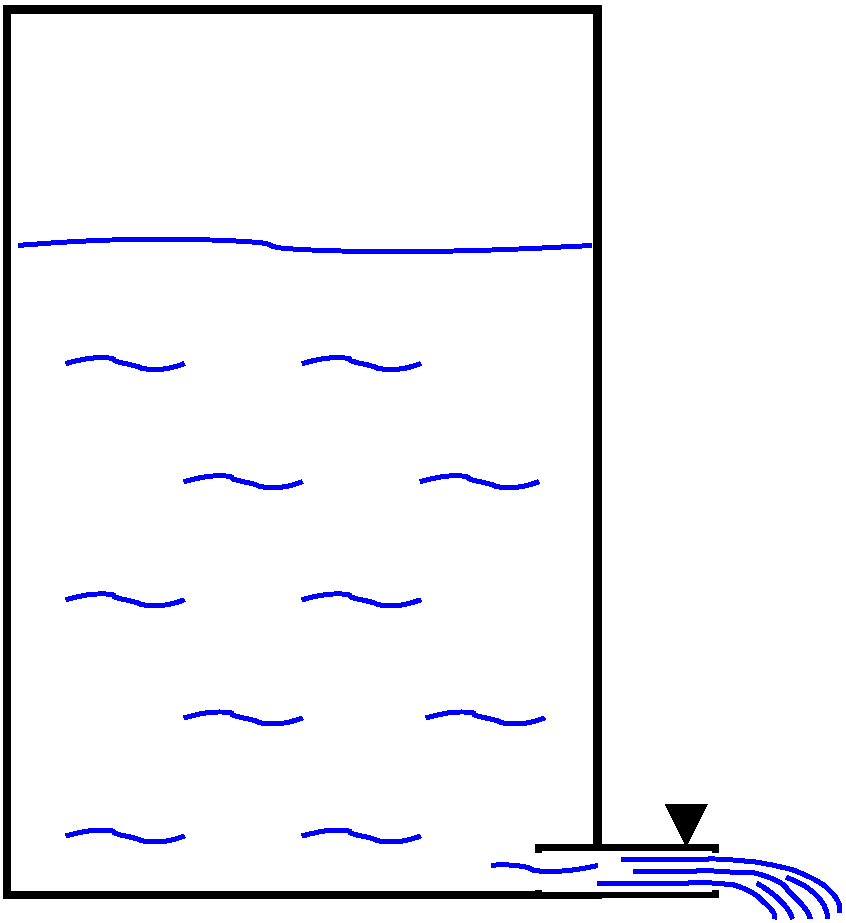
\includegraphics[width=0.9\textwidth]{./Figures/water_tank.pdf}
\end{minipage}

\medskip
From physical principles, one can derive the differential equation
\[ h'(t) = -\alpha \cdot \sqrt{h(t)} \]
for the height of the water level, where $\alpha$ is some positive constant that depends on the size of the tank and other parameters. This differential equation is known as Torricelli's law, and we will now learn how to solve it!
\end{application}


\section{First-Order Ordinary Differential Equations}
\label{sec:f-o}

\begin{definition}[ODEs, order, IVPs, solutions]
\label{def:f-o}
\begin{enumerate}[(i)]
	\item An \emph{ordinary differential equation (ODE)} is an equation involving an unknown function $y(x)$ and its derivatives
	\[ y'(x),\,y''(x),\,y'''(x),\,y^{(4)}(x),\,\dots,\,y^{(n)}(x) \]
	and other known functions of $x$.
	\item The order of the highest derivative appearing in an ordinary differential equation is called the \emph{order} of the ODE. For example, a first-order ODE is of the form
	\[ y' = f(x,y), \]
	where $f$ is a known function. The argument $x$ of $y$ is often omitted, but it is important to be aware that $y$ is a function.
	\item A first-order ODE together with an \emph{initial condition} of the form
	\[ y(x_0)=y_0, \]
	where the numbers $x_0,\,y_0$ are given, is called an \emph{initial-value problem (IVP)}.
	\item A function $y=y(x)$ that satisfies a given ODE is called a \emph{solution}. If $y$ contains parameters (constants) such that varying them covers all possible solutions to the ODE, then $y$ is called the \emph{general solution}. A solution that also satisfies given initial conditions is called a \emph{particular solution}. For now, i.e. until section~\ref{sec:pdes}, we can omit the specification 'ordinary'.
\end{enumerate}
\end{definition}

\begin{example}
\label{exple:first_de_exples}
\begin{enumerate}[(i)]
	\item The DE
	\[ y''(x)+4y(x)=0 \]
	has $y(x)=\sin(2x)$ as a solution. Indeed, we can check
	\begin{equation*}
	\begin{split}
	y(x) & =\sin(2x) \\
	\rightarrow \quad y'(x) & =2\cos(2x) \\
	\rightarrow \quad y''(x) & =-4\sin(2x) \\
	\rightarrow \quad y''(x) +4y(x) & = -4\sin(2x) + 4\sin(2x) = 0 \quad \text{\checkmark}.
	\end{split}
	\end{equation*}
	We will see later that the general solution is
	\[ y(x)=c_1\sin(2x)+c_2\cos(2x), \]
	which gives our guessed solution via the choice $(c_1,c_2)=(1,0)$ of constants.
	\item For the DE
	\[ y^{(4)} = 0, \]
	one can guess solutions $y(x)=1,\,y(x)=x^3,\,y(x)=2x^2-3x+5$, and hence the general solution
	\[ y(x) = Ax^3+Bx^2+Cx+D \]
	-- the polynomials of degree less than $4$.
\end{enumerate}
\end{example}

\begin{remark}
\label{rem:first_de_rems}	
\begin{enumerate}[(i)]
	\item As for integration: While solving DEs can be tricky, verifying solutions using differentiation is straightforward.
	\item Differential equations of the form
	\[ y'=f(x), \]
	i.e. when the function $f(x,y)$ in definition~\ref{def:f-o} (ii) does not depend on $y$, are the easiest to solve -- by integration:
	\[ y(x) = \itgr{}{}{f(x)}{x}. \]
	For example, the function $y(x)=\ln(x)+c$ solves the DE $y'=\rfrac1x$. We will refer to this type of DE as \emph{directly integrable}.
	\item The general solution of a $n$th-order DE usually contains $n$ constants. You can see that in the examples above. For directly integrable DEs, one can argue as follows: To solve
	\[ y^{(n)}=f(x), \]
	we integrate $f(x)$ $n$ times, obtaining a constant of integration each time. For this module, you can always work with the assumption that the general solution of a $n$th-order DE contains $n$ constants. Proving this for certain types of DEs -- it is not true for all DEs -- is beyond the scope of MTH1002.
	\item Our first non-trivial technique for solving ODEs is for those of the form
	\[ y'=h(x) \cdot g(y). \]
\end{enumerate}
\end{remark}

\subsection{Separable DEs}

\begin{example}
\begin{enumerate}[(i)]
	\item To solve the DE
	\[ y' = x \cdot y, \]
	we first write it as
	\[ \Df{y}{x} = x \cdot y \]
	and then \emph{separate variables}. That is, bring all expressions with an $x$ on one side and all expressions with $y$ on the other side. For that, we treat $dx$ like a number and 'multiply' the DE by it. Integrating gives
	\begin{equation}
	\label{eq:first_sop}
	 \itgr{}{}{\frac{1}{y}}{y} = \itgr{}{}{x}{x},
	\end{equation}
	which leads to
	\[ \ln\abs{y} = \frac{x^2}{2} + c_1 \qquad (c_1\in\mathbb{R}). \]
	Applying $\exp(.)$ on both sides gives
	\[ \abs{y} = \e^{\rfrac{x^2}{2}+c_1} = \e^{\rfrac{x^2}{2}}\,\e^{c_1} = c_2\, \e^{\rfrac{x^2}{2}} \qquad (c_2\in\mathbb{R}^+),\]
	where we let $c_2=\e^{c_1}$. Now, the absolute value on the left is either a factor of $+1$ or $-1$, depending on whether $y$ is positive or negative. Absorbing this potential negative sign into the constant, we have
	\[ y=c_3\,\e^{\rfrac{x^2}{2}} \qquad (c_3\in\mathbb{R}\backslash\{0\}). \]
	Even though $c_3 \not= 0$ is excluded, we note that a constant of $0$ works as well: Then we have $y(x)=0$ and 
	\[ y'(x) = 0 = x \cdot y. \]
	Hence we include the possibility $c=0$ and find the general solution to be
	\[ y(x) = c\,\e^{\rfrac{x^2}{2}} \qquad (c\in\mathbb{R}). \]
	
	Note that after~\eqref{eq:first_sop}, one should have stated that the function $y(x)$ can not have any zeros, since otherwise the integrand on the left-hand side would not be defined. Hence one solves the DE only on intervals on which $y$ is either always positive or always negative, and considers the case of $y$ having a zero separately. If $y(x_0)=0$, then $y'(x_0)=0$ by the original DE, and this suggests that the constant function $y(x)=0$ is a solution. Now, for the remaining cases, $y$ is either always positive or always negative, which allows to absorb the potential negative from $\abs{y}$ into the constant $c_2$. However, we will not always discuss the solution of DEs and the ranges of any constants involved that carefully. For example, in the next computation we might change the meaning of constants from one line to the next without explicitly renaming them.
	\item Solve the IVP
	\[ \left\{ \begin{split} 1+xyy' & = y^2+yy' \\ y(0) & = -\rfrac12. \end{split} \right. \]
	{\it Sol.:}
	\begin{equation*}
	\begin{split}
	\rightarrow & \quad (xy-y)\Df{y}{x} 
	= y^2-1 \quad \stackrel{\text{sep. of var.}}{\rightarrow} \quad
	\itgr{}{}{\frac{y}{y^2-1}}{y} = \itgr{}{}{\frac{1}{x-1}}{x} \\
	\stackrel{u=y^2-1}{\rightarrow} & \quad \frac12 \itgr{}{}{\frac1u}{u} = \ln\abs{x-1}+c \quad
	\stackrel{\text{integrate}}{\rightarrow} \quad \frac12\ln\abs{y^2-1} = \ln\abs{x-1} + c \\ 
	\stackrel{\cdot 2}{\rightarrow} & \quad \ln\abs{y^2-1} = \ln(x-1)^2+c \quad 
	\stackrel{\exp(.)}{\rightarrow} \quad \abs{y^2-1} = \e^{\ln(x-1)^2+c} \\
	\stackrel{\text{as in (i)}}{\rightarrow} & \quad y^2-1 = c\,(x-1)^2 \quad
	\rightarrow \quad y^2+c\,(x-1)^2=1.
	\end{split}
	\end{equation*}
	This is the general solution of the DE, but it is in implicit form, i.e. not solved for $y$ (it is not an explicit formula for $y(x)$). Next, we use the given initial data $(x_0,y_0)=(0,-\rfrac12)$:
	\[ \left(-\frac12\right)^2+c\,(0-1)^2 = \frac14+c\stackrel{!}{=} 1, \]
	which gives $c=\rfrac34$ and the explicit solution
	\[ y=\pm \sqrt{1-\rfrac34\,(x-1^2)}. \]
	For the particular solution to the given IVP, it remains to decide between $+$ and $-$. We choose
	\[ y(x) = -\sqrt{1-\rfrac34\,(x-1^2)} \]
	-- why not the positive solution\footnote{Check the initial condition for both possible choices.}?
\end{enumerate}
\end{example}

\begin{remark}
\label{rem:sov}
\begin{enumerate}[(i)]
	\item The implicit general solution $y^2+c\,(x-1)^2=1$ in (ii) describes an ellipse for $c>0$ (centred at $(1,0)$; a circle for $c=1$), a hyperbola for $c<0$, and a pair of horizontal lines for $c=0$.
	\item Next we study DEs of the form
	\[ \Df{y}{x} = f(x,y) = F\left(\rfrac{y}{x}\right),\]
	which we call \emph{homogeneous-type} and which can be transformed into separable DEs. A DE is homogeneous-type if 
	\[ f(\lambda x,\lambda y) = f(x,y) \qquad \text{for all~} \lambda\not=0. \]
\end{enumerate}
\end{remark}


\subsection{Homogeneous-Type}

\begin{example} Solve
	\[ \Df{y}{x}=\frac{x^2+y^2}{xy}. \]
{\it Sol.:} This DE is not separable. The expression on the right is invariant under replacing $x$ and $y$ with $\lambda x$ and $\lambda y$, respectively, so the DE is of homogeneous type. We solve it as follows:
\begin{equation}
\label{eq:homog1}
\Df{y}{x} = \frac{x^2\left( 1+\rfrac{y^2}{x^2} \right)}{x^2\:\rfrac{y}{x}}
= \frac{1+(\rfrac{y}{x})^2}{\rfrac{y}{x}} = F\left(\rfrac{y}{x}\right),
\end{equation}
where $F$ is the single-variable function defined by
\[ F(t) = \frac{1+t^2}{t}. \]
Set $t=\rfrac{y}{x}$, and note that it is a function of $x$: $t=t(x)$. Next, we find the relation between $y'$ and $t'$:
\begin{equation}
\label{eq:homog2}
 \Df{y}{x} = \Df{}{x}(x \cdot t ) = xt'+t.
\end{equation}
Combining \eqref{eq:homog1} and \eqref{eq:homog2}, we obtain a DE for $t(x)$:
\[ x\,t'+t=\frac{1+t^2}{t} \quad \rightarrow \quad x\,t'=\frac{1+t^2}{t}-t=\frac{1}{t}. \]
Writing this as
\[ x\,\Df{t}{x} = \frac{1}{t}, \]
we see that it is a separable DE, which we solve with the steps from the previous section:
\[ \itgr{}{}{t}{t} = \itgr{}{}{\frac{1}{x}}{x} \quad \rightarrow \quad
t^2 = \ln x^2+c = \left( \frac{y}{x} \right)^2, \]
which gives the general solution
\[ y(x) = \pm \, x \, \sqrt{\ln x^2+c}\,. \]
\end{example}

\subsection{Linear DEs}

\begin{definition}[Linear First-Order ODEs, Homogeneity]
\begin{enumerate}[(i)]
	\item A first-order ODE of the form
	\[ y'+p(x)\,y=r(x) \]
	is called \emph{linear}.
	\item It is further called \emph{homogeneous} if $r(x)=0$, and \emph{inhomogeneous} otherwise.
\end{enumerate}
\end{definition}

\begin{remark} Multiplying this DE by its \emph{integrating factor}
	\[ h(x):=\e^{P(x)}, \]
	where $P$ is any antiderivative of $p$, we obtain
	\[ h\,r =h\,y'+h\,p\,y= h\,y'+h'\,y = (h\,y)', \]
	which can be solved by integrating both sides:
	\[ h(x) \cdot y(x) = \itgr{}{}{h(x) \cdot r(x)}{x}. \]
\end{remark}

\begin{example}
\begin{enumerate}[(i)]
	\item Solve \[ y' +\frac{5}{x}\,y=\cos\left( x^6 \right).\]
	{\it Sol.:} The DE is linear, and the integrating factor 
	\[ h(x) = \e^{\itgr{}{}{\rfrac{5}{x}}{x}} = \e^{5\ln x} = x^5. \]
	Note that the constant of integration was omitted in the integration of $p(x)$ -- that is because the method using the integrating factor works for any antiderivative, and hence one can choose the easiest one: the antiderivative with $c=0$. Next, we find
	\[ x^5\,y=\itgr{}{}{x^5\,\cos\left(x^6\right)}{x} \stackrel{u=x^6}{=} \dots 
	= \frac16\left( \sin\left( x^6 \right) + c \right). \]
	Finally, dividing by the integrating factor gives the solution:
	\[ y(x)=\frac{\sin\left(x^6\right)+c}{6x^5}\,. \]
	\item Solve the IVP
	\[ \left\{ \begin{split}
	(1+x^2)y'-2xy&=1+x^2 \\ y(1)&=6.
	\end{split} \right. \]
	{\it Sol.:} First bring the DE in the correct form:
	\[ y'-\frac{2x}{1+x^2}y=1.\]
	Now one can read off the antiderivative $P(x)=-\ln(1+x^2)$ of $p(x)$. This gives the integrating factor
	\[ h(x)=\e^{-\ln(1+x^2)}=\frac{1}{1+x^2}, \]
	and therefore the general solution
	\[ y(x) = (1+x^2) \itgr{}{}{\frac{1}{1+x^2} \cdot 1}{x} 
	= (1+x^2)( \arctan x + c ).\]
	The initial condition gives
	\[ 6=(1+1^2)\left(\frac{\pi}{4}+c\right) \quad \rightarrow \quad
	y(x)=(1+x^2)\left( \arctan x + 3-\frac{\pi}{4} \right). \]
\end{enumerate}
\end{example}

\begin{application}[Logistic growth]
\texttt{\ldots}
\end{application}

\begin{exercise}
\begin{enumerate}[(i)]
	\item Work through the first-order DEs on the tutorial sheet for chapter~4.
	\item Letting $\alpha=1$ and $h(0)=100$, solve the differential equation for the water tank from the beginning of this chapter. Plot your solution -- does it make sense\footnote{Initially, it does not make sense, but setting the solution equal to $0$ from a certain $t_0$ on, one obtains a function for the water level $h(t)$ that does agrees with how one would imagine a tank to drain.}? How long does it take for the tank to drain\footnote{$20$ seconds.}?
	\item Solve\footnote{$y(x) \approx x \cdot \text{arcsin} ( \ln x + 0.866 )$,
	but you should obtain the constant exactly.}
	\[ xy'=y+x\sec\left(\frac{y}{x}\right), \quad y(1)=\frac{\pi}{3}.\]
	\item Solve\footnote{$y(x)=\frac{\sin^2x}{\cos x}$.}
	\[ y' = y \tan x + \sin x, \quad y(0)=0. \]
	\item Prove the statement from remark~\ref{rem:sov} (ii): Let $f(x,y)$ be a continuous function on $\mathbb{R}^2\backslash\{(0,0)\}$, i.e. $f$ is defined on the $xy$-plane without the origin $(x,y)=(0,0)$. There exists a single-variable function $F(t)$ such that 
	\[ f(x,y)=F(\rfrac{y}{x}) \]
	for any $x\not=0$, if and only if\footnote{Perhaps stating this more formally makes it more clear what needs to be done: Let $f=f(x,y)$ be continuous on $\mathbb{R}^2\backslash\{(0,0)\}$. Then
	\[ \exists \: F=F(t): f(x,y)=F(\rfrac{y}{x}) \: \forall x\not=0
	\: \Longleftrightarrow \: f(x,y)=f(\lambda x, \lambda y) \: \forall \lambda\not=0.
	\] The direction ``$\Longrightarrow$'' is the easier one. The case $x=0$ causes some extra work -- one can use continuity for that -- but it would be alright to skip this technicality.}
	\[ f(x,y) = f(\lambda x, \lambda y) \qquad \text{for all~}\lambda\not=0.\]
\end{enumerate}
\end{exercise}


\section{Linear Ordinary Differential Equations of Higher Order}
\label{sec:s-o}

\begin{definition}[Second-Order Linear ODEs]
	The standard form for a \emph{second-order linear ODE is}
	\[ y''+p(x)y'+q(x)y=r(x). \]
	A LODE is called homogeneous if $r(x)=0$, inhomogeneous otherwise.
\end{definition}

\begin{remark}
\label{rem:s-o_lode}
\begin{enumerate}[(i)]
	\item If we set
	\[ L[y]=y''+p(x)y'+q(x)y, \]
	the DE reads $L[y]=r(x)$. Here, $L$ is a \emph{differential operator} -- it takes a function as input and outputs a function. For example, the differential operator
	\[ \wtd{L}=7\Df{}{x} \]
	would map the input $x^2$ to $14x$.
	\item For LODEs: If $y_1,\,y_2$ are functions and $\alpha,\,\beta$ constants, then
	\[ L[\alpha y_1 + \beta y_2] = \alpha L[y_1] + \beta L[y_2]. \]
	\item If $y_1$ and $y_2$ are solutions to a homogeneous s-o LODE and they are \emph{linearly independent} (i.e. $y_2 \not= c \cdot y_1$), then
	\[ y(x) = c_1 y_1(x) + c_2 y_2(x) \]
	is the general solution.
	\item However, the previous statement, (iii), is not true in the inhomogeneous case: If
	\[ L[y_1] = r(x) \quad \text{and} \quad L[y_2] = r(x), \]
	then
	\[ L[y_1+y_2] = L[y_1] + L[y_2] = 2r(x), \]
	that is, $y_1+y_2$ does not satisfy $L[y]=r(x)$ (unless $r(x)=0$, which is the homogeneous case (iii)).
	\item The following technique allows us to find the general solution if one solution is known or can be guessed.
\end{enumerate}
\end{remark}

\subsection{Reduction of Order}

\begin{example}
Given the solution $y_1(x)=x$ of 
\[ x^2y''+xy'-y=0, \]
find $y_2$ and hence the general solution. \\
{\it Sol.:} First, one should verify that $y_1$ really is a solution:
\[ x^2y_1''+xy_1'-y_1=x^2 \cdot 0 + x \cdot 1 - x = x-x = 0 \quad \text{\checkmark}. \]
Now make the ansatz $y(x)=v(x) \cdot y_1(x)$, or, abbreviated, \[y=vy_1.\] The idea behind this ansatz is: the other solutions should be structurally similar to $y_1$, as they satisfy the same differential equation. From this viewpoint, it seems possible that using the knowledge of $y_1$ and analysing its ratio with other solutions might reduce the complexity of the problem. We have
\[ y=vy_1,\quad y'=v'y_1+vy_1', \quad y''=v''y_1+2v'y_1'+vy_1'', \]
and therefore
\begin{equation*}
\begin{split}
L[y] & = L[vy_1] = x^2 \cdot \left[ v''y_1+2v'y_1'+vy_1'' \right]
+ x \cdot \left[ v'y_1+vy_1' \right] - \left[ vy_1 \right] \\
& = x^2v''y_1+2x^2v'y_1'+xv'y_1+v \cdot
\underbrace{\left[ x^2y_1''+xy_1'-y_1 \right]}_{=L[y_1]=0} \\
& = x^2v''y_1+2x^2v'y_1'+xv'y_1+v \cdot 0 \qquad (\text{now use~} y_1=x,\,y_1'=1,\,y_1''=0) \\
& = x^3v''+3x^2v' \stackrel{w=v'}{=} x^3w'+3x^2w \stackrel{!}{=} 0.
\end{split}
\end{equation*}
That is, if $w=w(x)$ satisfies the first-order LODE
\[ x^3w'+3x^2w = 0, \]
then $y=vy_1$ will satisfy the original second-order LODE. We find
\begin{equation*}
\begin{split}
w(x) &= \frac{\alpha}{x^3}, \\
v(x) &= -\frac{\alpha}{2}x^{-2} + \beta, \\
y(x) &= \beta x - \frac{\alpha}{2} \frac{1}{x},
\end{split}
\end{equation*}
where $\alpha, \beta \in \mathbb{R}$, and, after renaming the constants,
\[ y(x) = c_1 \cdot x + c_2 \cdot \frac{1}{x}. \]
This is the general solution of the DE, and it is in the form mentioned in remark~\ref{rem:s-o_lode} (iii), with $y_2=\rfrac{1}{x}$.
\end{example}

\begin{remark}
We recommend writing out $L[y]=L[vy_1]=\dots$ as above, rather than using the formula for $y_1$, which is already known at this point. Then, \emph{after} the term $v \cdot L[y_1]$ has dropped out of the computation, one can substitute in the formula for $y_1$ and its derivatives. Using the formula for $y_1$ from the beginning, i.e. $L[y]=L[v \cdot x]=\dots$ in this case, would often make the computation more complicated, e.g. if $y_1$ is a rational function with bulky derivatives. 
\end{remark}

\subsection{Constant-Coefficient Homogeneous}
\label{sec:cch}

\begin{remark} Consider the second-order LODE
\label{rem:cch}
	\begin{equation}
	\label{eq:char_eq1}
		L[y] = y''+py'+qy = 0,
	\end{equation} 
	where $p,\,q$ are \emph{constants}, not functions of $x$. Making the ansatz
	\[ y(x) = \e^{\lambda x}, \]
	we find
	\[	0  \stackrel{!}{=} L[\e^{\lambda x}]
	= \Ddf{}{x} \left( \e^{\lambda x} \right) +
	p\,\Df{}{x} \left( \e^{\lambda x} \right) + q\,\e^{\lambda x} 
	= \e^{\lambda x}\left(\lambda^2+p\,\lambda+q\right). \]
	That is, if $\lambda$ satisfies the \emph{characteristic equation} (or \emph{auxiliary equation})
	\begin{equation}
	\label{eq:char_eq2}
		\lambda^2+p\,\lambda+q = 0,
	\end{equation}
	then $y=\e^{\lambda x}$ is a solution of~\eqref{eq:char_eq1}. The solutions of~\eqref{eq:char_eq2} are
	\[ \lambda_{1/2} = \frac{-p\pm\sqrt{p^2-4q}}{2}, \]
	and we now have to consider three cases:
	\begin{enumerate}[(I)]
		\item If~\eqref{eq:char_eq2} has two distinct real solutions $\lambda_1$ and $\lambda_2$ -- this happens when $p^2-4q>0$ -- then we have solutions
		\[ y_1(x) = \e^{\lambda_1 x}, \qquad y_2(x) = \e^{\lambda_2 x}, \]
		of~\eqref{eq:char_eq1}. From earlier theory, we conclude that the general solution is
		\[ y(x) = c_1\,\e^{\lambda_1 x} + c_2\,\e^{\lambda_2 x}.\]
		\item If~\eqref{eq:char_eq2} has one real solution $\lambda$ (i.e. a double root, $\lambda_1=\lambda_2$) -- this happens when $p^2-4q=0$ -- then we have solutions
		\[ y_1(x) = \e^{\lambda x}, \qquad y_2(x) = x\,\e^{\lambda x}. \]
		That $y_1$ is a solution follows again from $\lambda$ solving the characteristic equation, and $y_2$ is obtained via reduction of order. Note that $\lambda=-\rfrac{p}{2}$ in this case. The general solution is
 		\[ y(x) = c_1\,\e^{\lambda x} + c_2\,x\,\e^{\lambda x}. \]
		\item If~\eqref{eq:char_eq2} has no real solutions -- this happens when $p^2-4q<0$ -- then it has complex solutions 
		\[ \lambda_{1/2} = a \pm ib \qquad (a,b\in\mathbb{R}), \]
		and the solutions to the differential equation are
		\[ y_1(x) = \e^{ax}\cos(bx), \qquad y_2(x) = \e^{ax}\sin(bx). \]
		The derivation of this is outlined in the exercises below. The general solution is
		\[ y(x) = \e^{ax}\left[ c_1\cos(bx)+c_2\sin(bx) \right]. \]
\end{enumerate}
\end{remark}

\begin{definition}[IVPs and BVPs]
	For a second-order ODE, $L[y] = r(x)$,
	the system of equations
	\begin{equation*}
	\left\{
	\begin{split}
L[y] &= r(x) \\ y(a) &= A \\ y'(a) &= B 
	\end{split}\right.
	\end{equation*}
	is called an \emph{initial-value problem} (IVP). A system of the form
	\begin{equation*}
	\left\{
	\begin{split}
L[y] &= r(x) \\ y(a) &= A \\ y(b) &= B 
	\end{split}\right.
	\end{equation*}
	is called an \emph{boundary-value problem} (BVP).
\end{definition}

\begin{example}
\label{expl:bvps_ivps}
\begin{enumerate}[(i)]
	\item
	\[ \left\{ 
	\begin{split}
		y''-3\,y'+\rfrac{9}{4}\,y & = 0 \\ 
		y(0) & = 0 \\ y\left(\rfrac{2}{3}\right) & = 1
	\end{split}
	\right.\]
	{\it Sol.:} We first consider the DE only, which is second-order, linear, and homogeneous with constant coefficients. Its characteristic equation is
	\[ 0 = \lambda^2-3\lambda+\frac94 = (\lambda-\rfrac32)(\lambda-\rfrac32), \]
	which has the double root $\lambda=\rfrac32$, i.e. we have case (II) from the discussion above. This value of $\lambda$ implies that the general solution is
	\[ y(x) = c_1\,\e^{\rfrac32\,x} + c_2\,x\,\e^{\rfrac32\,x}, \]
	and it remains to determine the constants so that $y$ satisfies the given boundary conditions:
	\[ \begin{split}
	0 \stackrel{!}{=} y(0) & = c_1\cdot1 +c_2\cdot0\cdot1 = c_1 \\
	1 \stackrel{!}{=} y\left( \rfrac23 \right) 
		& = c_1 \cdot \e + c_2 \cdot \rfrac23 \cdot \e = \rfrac{2\e}{3}\,c_2,
	\end{split}\]
	which leads to the particular solution 
	\[ y(x) = \frac{3x}{2\e}\,\e^{\rfrac23\,x}. \]
	\item
		\[ \left\{ 
	\begin{split}
			y''-y'+\rfrac{17}{4}\,y & = 0 \\ 
			y(0) & = 0 \\ y'(0) & = 10
	\end{split}
	\right.\]
	{\it Sol.:} 
	The characteristic equation is 
	\[ \lambda^2-\lambda +\frac{17}{4} = 0, \]
	which has solutions
	\[ \lambda_{1/2} = \frac{-(-1)\pm\sqrt{(-1)^2-4 \cdot \rfrac{17}{4}}}{2}
	= \frac12 \pm \frac{\sqrt{-16}}{2} = \frac12 \pm i \cdot 2, \]
	and therefore leads to the general solution
	\[ y(x) = \e^{\rfrac{x}{2}}\left( c_1\cos(2x) + c_2\sin(2x) \right). \]
	In order to find the solution of the IVP, we need to set the values of $y$ and $y'$ at $x=0$ equal to the given values. Therefore, $y'(x)$ needs to be found:
	\[ y'(x) = \frac12\e^{\rfrac{x}{2}}\left( c_1\cos(2x) + c_2\sin(2x) \right)
	+\e^{\rfrac{x}{2}}\left(-2c_1\sin(2x) + 2c_2\cos(2x) \right).\]
	Now we can solve for the constants:
	\[ \left\{ \begin{split}
	0=y(0)&=\e^0 (c_1\cos 0 + c_2\sin 0) = c_1 \\
	10=y'(0)&=\rfrac12\,\e^0(c_1\cos 0 + c_2\sin 0)
	+ \e^0 (-2c_1\sin 0 + 2c_2\cos 0)=\rfrac{1}{2}\,c_1+2c_2,
	\end{split}\right.\]
	which gives $c_1=0,\,c_2=5$ and hence
	\[ y(x) = 5\,\e^{\rfrac{x}{2}}\sin(2x). \]
	\item
	\[\left\{ \begin{split}
	y''+y'-6y &= 0 \\ y(0) &= 1 \\ y'(0) &= 12
	 \end{split}\right.\]
	{\it Sol.:} 
	\[ y(x) = 3\,\e^{2x}-2\,\e^{-3x}\]
\end{enumerate}
\end{example}

\begin{remark}
\begin{enumerate}[(i)]
	\item At the beginning of this chapter, in remark~\ref{rem:first_de_rems}, it was stated that the general solution of a $n$th-order DE contains $n$ constants. From this, one can deduce that it takes $n$ conditions to specify a particular solution -- this agrees with the examples we have seen so far: one condition in section~\ref{sec:f-o} and two conditions (either IVP or BVP) for the second-order DEs in the previous example.
	\item The difference between an IVP and an BVP can be illustrated as follows. Many natural processes obey second-order differential equations, and the motion of objects is a prominent example. Suppose a ball is kicked vertically in the air, and you are shown a snapshot of it. That is, you are given the height at a certain time, $h(t_1)$. From this, you cannot say what will happen next -- for example, you do not know whether the ball was on its way up or down when the picture was taken. However, if you are given a second piece of information, you can -- with your knowledge from this module -- determine the exact trajectory $h(t)$ of the ball. This second piece of information could be the velocity $h'(t_1)$ of the ball ($\rightarrow$ IVP; how fast and in which direction was it moving when the picture was taken) or the position at some other specified time ($\rightarrow$ BVP; e.g., another snapshot, taken exactly one second later).
	\item The method of using the characteristic equation remains applicable for LODEs of higher orders -- however, then the characteristic equation will be of higher order as well, and it might therefore not be readily solvable. Sometimes, one is able to guess one solution and then reduce its order, cf. the next example.
\end{enumerate}
\end{remark}

\begin{example}
\[ y''' - \frac12 \, y'' -\frac{41}{2} \, y' + 35 \, y = 0 \]
{\it Sol.:} The characteristic equation is 
\[ \lambda^3 - \frac12 \, \lambda^2 -\frac{41}{2} \, \lambda + 35 = 0, \]
and after some experimentation, one finds the solution $\lambda = 2$, since $8-2-41+35=0$.  This means that $(\lambda-2)$ is a factor of the cubic expression on the left -- dividing by it (long division of polynomials), we obtain
\[ 0 = \lambda^3 - \frac12 \, \lambda^2 -\frac{41}{2} \, \lambda + 35 
= (\lambda-2)\left( \lambda^2+\frac32\lambda-\frac{35}{2} \right) = (\lambda-2)(\lambda-\rfrac{7}{2})(\lambda+5),\]
and therefore the general solution
\[ y(x) = c_1\,\e^{2x} + c_2\,\e^{\rfrac{7}{2}x} + c_3\,\e^{-5x}. \]
\end{example}

\subsection{Constant-Coefficient Inhomogeneous}

\begin{remark}
\begin{enumerate}[(i)]
	\item The steps for solving an \emph{inhomogeneous} linear second-order DE with constant coefficients, 
	\[ L[y] = y''+py'+qy = r(x), \qquad \qquad p,\,q\in\mathbb{R},\]
	are:
	\begin{enumerate}[(1)]
		\item Solve the corresponding homogeneous DE, $L[y] = 0$. Its general solution is called the \emph{complementary function}:
		\[ y_{CF} = c_1y_1+c_2y_2. \]
		\item Find one solution of the inhomogeneous DE, $L[y]=r(x)$. This solution is denoted $y_{PI}$ and called the \emph{particular integral}. Finding $y_{PI}$ will be discussed below.
		\item The general solution of the inhomogeneous DE is
		\[ y = y_{CF} + y_{PI} = c_1y_1+c_2y_2 + y_{PI}. \]
		\item If the DE was given as an IVP or a BVP, i.e. with two additional conditions, then determine the constants in the general solution (3) so that the resulting function satisfies those conditions. This function is the solution to the IVP/BVP.
	\end{enumerate}
	\item Let us check whether the function from step (3) above really is the general solution of $L[y]=r(x)$: The function
	\[ y = y_{CF} + y_{PI} = c_1y_1+c_2y_2 + y_{PI} \]
	does contain two constants -- as we expect for the general solution of a second-order DE -- and
	\begin{equation*}
	\begin{split}
	L[y] = L[c_1y_1+c_2y_2 + y_{PI}] &= c_1L[y_1] + c_2L[y_2]+L[y_{PI}] \\ 
	&= c_1 \cdot 0 + c_2 \cdot 0 + r(x) = r(x) \quad \text{\checkmark}.
	\end{split}
	\end{equation*}
\end{enumerate}
\end{remark}

\begin{example}
Solve the IVP
\[ \left\{ \begin{split}
y''-y'-12y & = \e^{2x} \\ y(0) & = -2 \\ y'(0) & = 2
\end{split} \right. .\]
{\it Sol.:}
\begin{enumerate}[(1)]
	\item First we consider the homogeneous version of the DE,
	\[ y''-y'-12y = 0. \]
	Its characteristic equation is
	\[ 0 = \lambda^2-\lambda-12 = (\lambda-4)(\lambda+3), \]
	and it leads to the two solutions 
	\[ y_1(x) = \e^{4x}, \qquad y_2(x) = \e^{-3x}, \]
	of the homogeneous DE. Hence the complimentary function is
	\[ y_{CF}(x) = c_1 \, \e^{4x} + c_2 \, \e^{-3x}. \]
	\item Next, we need one solution of the inhomogeneous DE, the particular integral, $y_{PI}$. The idea is to make an ansatz containing parameters for it and then substitute it into $L[y]=\e^{2x}$ to determine those parameters. Choosing the correct form for $y_{PI}$ is key:
	\begin{enumerate}[{Attempt} 1:]
		\item Take $y_{PI}(x)=\sqrt{Ax^2+Bx+C}$. However, thinking about the action of the operator $L$, we see that 
		\[ \begin{split}
L[y_{PI}]&=L\left[\sqrt{Ax^2+Bx+C}\right] \\
&=\Ddf{}{x}\left[\sqrt{Ax^2+Bx+C}\right]-\Df{}{x}\left[\sqrt{Ax^2+Bx+C}\right] \\
& \qquad \quad \qquad \qquad \qquad \qquad -12\left[\sqrt{Ax^2+Bx+C}\right] = \dots
		\end{split}  \]
		will not lead to an expression that can be made equal to $\e^{2x}$ by making suitable choices for $A,\,B,\,C$.
		\item For $y_{PI}(x) = A\cos x +B\sin x$, application of $L$ will give a combination of trigonometric functions $\cos x$ and $\sin x$, not $\e^{2x}$.
		\item The previous attempts suggest that one should make an ansatz of the same form as the inhomogeneity $r(x)$. Hence try $y_{PI}(x) = A\e^{2x}$:
		\[ L[y_{PI}]=L\left[ A\e^{2x} \right] 
		= A \left[ 4 \e^{2x} - 2 \e^{2x} - 12 \e^{2x} \right] 
		= A (-10) \e^{2x} \stackrel{!}{=}\e^{2x},\]
		and therefore $A=\rfrac{-1}{10}$,
		\[ y_{PI}(x) = \frac{-1}{10}\e^{2x}. \]
		General advice on how to make the ansatz for the particular integral will be given below.
	\end{enumerate}
	\item The general solution of the original inhomogeneous DE is
			\[ y = y_{CF} + y_{PI} = c_1\,\e^{4x}+c_2\,\e^{-3x} - \frac{1}{10}\,\e^{2x}. \]
	\item The initial conditions give rise to the system 
	\[ \left\{ \begin{split}
		-2 = y(0) & = c_1+c_2-\rfrac{1}{10} \\
		2 = y'(0) & = 4c_1-3c_2-\rfrac{2}{10},
	\end{split} \right. \]
	which has solutions $c_1=-\rfrac12,\,c_2=-\rfrac{7}{5}$. This gives the solution to the IVP as
	\[ y = -\frac12\,\e^{4x}-\frac{7}{5}\,\e^{-3x} - \frac{1}{10}\,\e^{2x}. \]
\end{enumerate}
\end{example}

\begin{remark}
\label{rem:inhomog}
\begin{enumerate}[(i)]
	\item The following table and remarks should help you make the ansatz for the particular integral:
	\begin{center}
		\begin{tabular}{ | c | c | }
			Right-hand side $r(x)$ & Ansatz for $y_{PI}$ \\ \hline \hline
			polynomial of degree $m$: & polynomial of degree $m$: \\ 
			$\alpha_m x^m + \dots \alpha_1 x + \alpha_0$ 
			& $A_m x^m + \dots A_1 x + A_0$ \\ \hline
			exponential: & exponential: \\ 
			$\alpha\e^{\lambda x}$ & $A\e^{\lambda x}$ \\ \hline
			comb. of trig. functions: & comb. of trig. functions: \\
			$\alpha \cos(\lambda x) + \beta \sin(\lambda x)$ &
			$A\cos(\lambda x) + B\sin(\lambda x)$ \\ \hline 
			\ldots & \ \ldots \\
			(e.g.: comb. of hyp. trig. fcns & comb. of hyp. trig. fcns) \\ \hline
			a sum of any of the above: & find $y_{PI,j}$ for each $r_j$ and then: \\
			$r(x) = r_1(x) + \dots + r_k(x)$ &
			$y_{PI} = y_{PI,1} + \dots + y_{PI,k}$  \\ \hline
		\end{tabular}
	\end{center}
	Here it is important to always have full generality on the ansatz side: E.g., if $r(x)=2\sin(3x)$, i.e. there is no $\cos(3x)$ term in the inhomogeneity, one still needs $y_{PI}=A\cos(3x) + B\sin(3x)$ rather than an ansatz with a sine term only. If, for example, $r(x)=\sin(5x)+\cos(2x)$, the rule in the middle row of the table needs to be applied twice -- once for $\lambda=5$ and once for $\lambda=2$ -- and the outcomes are then to be combined as in the last row. If you have written out the ansatz $y_{PI}$ based on $r(x)$, but this $y_{PI}$ happens to already be a solution to the homogeneous version of the DE, then multiply it by~$x$.
	\item The linearity of the ODE is crucial for the above approach of finding all solutions of the homogeneous DE and then adding one solution of the inhomogeneous DE. Let us compare this to another linear situation: An inhomogeneous linear equation for the variables $x,\,y,\,z$: Solve 
	\begin{equation}
	\label{eq:plane}
	x+2y-5z = 2. 
	\end{equation}
	{\it Sol.:} 
	\begin{enumerate}[(1)]
		\item For the homogeneous version of the equation,
		\[ x+2y-5z = 0, \]
		we can find the two linearly independent (cf. \ref{def:li} for the general definition of this term) solutions
		\[ v_1 = \begin{bmatrix} 5 \\ 0 \\ 1\end{bmatrix}, \qquad 
		   v_2 = \begin{bmatrix} 0 \\ 5 \\ 2\end{bmatrix} \]
		and hence the general solution 
		\[ v_{CF} = c_1 \begin{bmatrix} 5 \\ 0 \\ 1\end{bmatrix}
		+ c_2 \begin{bmatrix} 0 \\ 5 \\ 2\end{bmatrix}. \]
		\item We now just need a single vector that satisfies the inhomogeneous equation~\eqref{eq:plane}. For example, 
		\[ v_{PI} = \begin{bmatrix} 2 \\ 0 \\ 0 \end{bmatrix}, \]
		as
		\[ \begin{bmatrix}	1 & 2 & -5 \end{bmatrix}
		\begin{bmatrix} 2 \\ 0 \\ 0	\end{bmatrix} = 2 \quad \text{\checkmark} \]
		(the entries of the row vector are the coefficients of \eqref{eq:plane}).
		\item The general solution of the inhomogeneous equation is
				\[ v = \begin{bmatrix} 2 \\ 0 \\ 0 \end{bmatrix} +
				c_1 \begin{bmatrix} 5 \\ 0 \\ 1\end{bmatrix}
		+ c_2 \begin{bmatrix} 0 \\ 5 \\ 2\end{bmatrix}. \]
		This is a parametrisation of the plane~\eqref{eq:plane}.
\end{enumerate} 
\end{enumerate}
\end{remark}

\begin{example}
Find the general solution of 
\[ L[y] = y''-3\,y'+\rfrac{9}{4}\,y = \e^{\rfrac{3x}{2}}. \]
{\it Sol.:}
\begin{enumerate}[(1)]
	\item We have already found the solution to the homogeneous version of that DE in example~\ref{expl:bvps_ivps} (i):
	\[ y_{CF}(x) = c_1\,\e^{\rfrac32\,x} + c_2\,x\,\e^{\rfrac32\,x}. \]
	\item Based on the form of the right-hand side, $r(x)=\e^{\rfrac{3x}{2}}$, one would make the ansatz $y_{PI}=A\e^{\rfrac{3x}{2}}$. However, this will be mapped to $0$ by $L$, as it is a solution of $L[y]=0$ -- after all, the function $A\e^{\rfrac{3x}{2}}$ is already contained in the complementary function; for $(c_1,c_2)=(A,0)$. According to the last sentence of remark~\ref{rem:inhomog} (i), we multiply by $x$ to obtain $y_{PI}=Ax\e^{\rfrac{3x}{2}}$. Again, this already solves the homogeneous DE, and we therefore multiply by $x$ one more time:
	\[ y_{PI}(x)=Ax^2\e^{\rfrac{3x}{2}}. \]
	Substituting this into $L[y]=\e^{\rfrac{3x}{2}}$ gives
	\begin{equation*}
	\begin{split}
	 L\left[ Ax^2\e^{\rfrac{3x}{2}} \right] 
	 &= A\left[ 2\e^{\rfrac{3x}{2}} + 6x\e^{\rfrac{3x}{2}} 
	 + \frac{9}{4}x^2\e^{\rfrac{3x}{2}} \right] \\
	 & \qquad -3A\left[ 2x\e^{\rfrac{3x}{2}} + \frac{3}{2}x^2\e^{\rfrac{3x}{2}} \right]
	 +\frac{9}{4}A\left[ x^2\e^{\rfrac{3x}{2}} \right] \\
	 & = A \left[ 2 + 6x + \frac94x^2 - 6x -\frac92x^2 + \frac94x^2  \right] \e^{\rfrac{3x}{2}}
	 =2A\e^{\rfrac{3x}{2}} \stackrel{!}{=} \e^{\rfrac{3x}{2}},
	\end{split}
	\end{equation*}
	and hence
	\[ y_{PI}(x)=\frac{x^2}{2}\e^{\rfrac{3x}{2}}. \]
	\item Steps (1) and (2) lead to the general solution
	\[ y(x) = \e^{\rfrac{3x}{2}}\left( c_1+c_2x+\frac{x^2}{2} \right). \]
\end{enumerate}
\end{example}

\begin{exercise}
\begin{enumerate}[(i)]
		\item Solve the higher-order ODEs on the tutorial sheet.
		\item Consider the s-o LODE	\[y''+4y=0\]
		from example~\ref{exple:first_de_exples} and the solution $y_1(x)=\sin(2x)$ we had already guessed and verified. Using reduction of order, find the general solution. Then also solve the DE using the theory from section~\ref{sec:cch}.
		\item Solve the BVP\footnote{The general solution is $y_{\text{gen}}(x)= A \, \e^x \cos x + B \, \e^x \sin x + 5$, and you can verify the constants you have found for the particular solution by checking whether it satisfies the boundary conditions.} 
		\[ \left\{\begin{split}
			y''-2y'+2y & = 10 \\ y(0) & = 7 \\ y(\rfrac{\pi}{2}) & = 4.
		\end{split}\right. \]
		\item Find the general solution of\footnote{$y(x)=A\,\e^{-x}+B\,x\e^{-x}+\rfrac{1}{2}\,x^2\e^{-x}
			+\rfrac{5}{32}\cosh(3x)-\rfrac{3}{32}\sinh(3x)$, where the hyperbolic functions could also be written out as a sum of exponential expressions.} 
		\[ y''+2y'+y=\cosh(3x)+\e^{-x} .\]
		\item Consider the s-o LODE
		\begin{equation}
		\label{eq:DE_two_methods}
		L[y] = x^3 y'' + 3 x^2 y' + x y = 0.
		\end{equation}
		Find one solution via the ansatz $y_1(x) = x^r$, and then find the general solution via reduction of order.
		\item Solve the DE \eqref{eq:DE_two_methods} again, this time by transforming to a DE for the function $u=u(t)$, where $u = x \cdot y$ and $x=\e^t$.
		\item  Show that the function $y_2$ in (II) of remark~\ref{rem:cch} and both functions $y_{1/2}$ in (III) really are solutions of~\eqref{eq:char_eq1} in the respective cases. The former can be done with reduction of order, and	the latter by carrying out (I) for complex $\lambda$, e.g. $y_1=\e^{(a+ib)x}$ -- the usual argument involving the characteristic equation remains applicable, and the laws of exponentials are true in the complex case as well -- and then using \emph{Euler's identity},
		\[ \e^{ix} = \cos(x)+i\sin(x) \]
		and renaming the constants. A different approach would be, of course, to simply verify that the functions that are given satisfy the constant-coefficient homogeneous second-order LODE~\eqref{eq:char_eq1}. Euler's identity is very significant and perhaps surprising: for $x=\pi$ we obtain
		\[ \e^{i\pi} = -1, \]
		combining three important mathematical constants on the left -- that are quite non-trivial (irrational/imaginary) and seemed unrelated until now -- to a rather simple number on the right.
\end{enumerate}
\end{exercise}


\section{Partial Differential Equations}
\label{sec:pdes}

\begin{remark}
\emph{Partial differential equations} (PDEs) are differential equations for multivariate functions, i.e. equations involving the partial derivatives of an unknown function. Many natural processes obey partial differential equations, for example: The temperature in a room as a function of time can be modelled with 
\[ u = u(t,x,y,z) \]
and satisfies the \emph{heat equation}
\[ u_t-\alpha\left( u_{xx}+u_{yy}+u_{zz}\right) = 0.\]
The heat equation is a very important PDE. We will not be able to discuss it in MTH1002, but you will learn how to solve it in MTH2003.
\end{remark}

\begin{example}
\begin{enumerate}[(i)]
	\item Solve the PDE \[ \df{u}{x} = 0, \] where $u=u(x,y)$.\\
	{\it Sol.:}
	Let us just integrate that equation with respect to $x$:
	\[ \itgr{}{}{\df{u}{x}}{x} = u = \itgr{}{}{0}{x} = c(y). \]
	Here, the constant of integration can be a function of $y$, since any expression that does not depend on $x$ has $0$ as its $x$-derivative. Renaming the ``constant'', we find the solution
	\[ u(x,y) = w(y), \]
	where $w$ is an arbitrary differentiable single-variable function. Since this is a new type of computation, and since it might be surprising to have so much freedom of choice in the general solution -- for first-order ODEs, that would be a constant; here it is a function that can be chosen freely -- let us check: 
	\[ \df{u}{x} = \df{}{x} \left( w(y) \right) = 0 \quad \text{\checkmark}. \]
	\item \[ \dff{u}{x}{y} = 0 \]
	{\it Sol.:}
	\begin{equation*}
	\begin{split}
	\df{}{x}\left(\df{u}{y}\right) = 0 \qquad & \stackrel{\itgr{}{}{\cdot}{x}}{\rightarrow} \qquad 
	\df{u}{y} = \itgr{}{}{0}{x} = w(y) \\
	& \stackrel{\itgr{}{}{\cdot}{y}}{\rightarrow} \qquad u = \itgr{}{}{w(y)}{y} 
	\stackrel{W'=w}{=} W(y) + v(x) \\
	& \stackrel{\text{rename}}{\rightarrow} \qquad u(x,y) = f(x) + g(y),
	\end{split}
	\end{equation*}
	where $f$ and $g$ are arbitrary differentiable single-variable functions. Check this result using partial differentiation!
\end{enumerate}
\end{example}

\begin{remark}
\begin{enumerate}[(i)]
	\item As hinted on above, the set of solution is \emph{much} bigger for PDEs than for ODEs of the same order. You will see that when solving the exercises below and the PDEs on the tutorial sheet.
	\item The previous examples are analogous to directly integrable ODEs -- they can be solved directly using integration. The next example can not be solved as readily, but we will bring it into directly integrable form using theory from chapter~\ref{ch:fsv}.
\end{enumerate}
\end{remark}

\begin{example}
Find $u=u(x,y)$ that satisfies
\[ L[u] = 6\ddf{u}{x} + \dff{u}{x}{y} - \ddf{u}{y} = 0. \]
	{\it Sol.:}
Note that we can not simply integrate the PDE, as $L[u]$ is a sum of different partial derivatives of $u$. The idea is to define new variables,
\[ \xi = x+ay,\qquad \eta=x+by, \qquad \qquad
(\xi\rightarrow\text{``xi''},\,\eta\rightarrow\text{``eta''})\]
and then choose the parameters $a$ and $b$ so that the PDE can be integrated directly in the new variables (we had already carried out such a transformation in chapter 2: example~\ref{expl:chain_rule_ii} (iv)). The partials transform as follows:
\begin{equation*}
\begin{split}
\df{u}{x} &= u_\xi+u_\eta, \qquad
\df{u}{y} = a\,u_\xi+b\,u_\eta, \\
\ddf{u}{x} &= u_{\xi\xi}+2\,u_{\xi\eta}+u_{\eta\eta}, \\
\ddf{u}{y} &= a^2\,u_{\xi\xi}+2ab\,u_{\xi\eta}+b^2\,u_{\eta\eta}, \\
\dff{u}{x}{y} &= a\,u_{\xi\xi}+(a+b)\,u_{\xi\eta}+b\,u_{\eta\eta}, 
\end{split}
\end{equation*}
and hence $L[u]$ transforms to 
\begin{equation*}
\begin{split}
L[u] &= 6\,u_{\xi\xi}+12\,u_{\xi\eta}+6\,u_{\eta\eta}
+ a\,u_{\xi\xi}+(a+b)\,u_{\xi\eta}+b\,u_{\eta\eta}
- a^2\,u_{\xi\xi}-2ab\,u_{\xi\eta}-b^2\,u_{\eta\eta} \\
&= \left[ 6+a-a^2 \right]u_{\xi\xi} + \left[ 12+a+b-2ab \right]u_{\xi\eta}
+\left[ 6+b-b^2 \right]u_{\eta\eta} \\
&=: c_1\,u_{\xi\xi} + c_2\,u_{\xi\eta} + c_3\,u_{\eta\eta}
\stackrel{!}{=} c \cdot u_{\xi\eta}.
\end{split}
\end{equation*}
The last line states that we assigned the names $c_1,\,c_2,\,c_3$ to the expressions in square brackets in the previous line. We would then like this combination of second-order partials with respect to $\xi$ and $\eta$ to be of the form some constants times $u_{\xi\eta}$, as this is a PDE that we can solve, cf. the previous example. For $L[u]=0$ to be equivalent to $u_{\xi\eta}=0$, we need $c_1=0$, $c_3=0$, and $c_2\not=0$, because then
\[ L[u]=0 \quad \Longleftrightarrow \quad c_2\,u_{\xi\eta}=0
\quad \Longleftrightarrow \quad u_{\xi\eta}=0. \]
Setting $c_1=0$ and $c_3=0$ leads to
\[ a\in \{-2,3\} \quad \text{and} \quad b\in\{-2,3\},  \]
which a-priori leaves four choices for the combination of parameters $(a,b)$. However, if $a=b$, then
\[ c_2 = 12+2a-2a^2 = 2[6+a-a^2]=2 \cdot 0 = 0, \]
which shows that $a=b$ is not a suitable choice. (If we chose $a=b$, we would have $\xi=\eta$, and we would therefore be looking for functions that can effectively be written as functions of one variable -- this would not give us full generality for solutions of $L[u]=0$.) We are left with two equivalent choices for $(a,b)$. Take 
\[ \xi = x+3y, \qquad \eta = x-2y. \]
The new DE is
\[ u_{\xi\eta} = 0, \]
which we have already solved in the previous example (well, the variables were called $x$ and $y$ then). Its solution is $f(\xi)+g(\eta)$, and we therefore obtain the solution
\[ u(x,y) = f(x+3y)+g(x-2y) \]
in the original variables. Here, $f$ and $g$ are arbitrary single-variable functions (twice differentiable).
\end{example}

\begin{application}[Wave equation]
\texttt{Stone dropped in a swimming pool, do quickly, use Fourier theory from the previous chapter to find correct superposition of modes; mention heat equation and Black-Scholes as other applications.}
\end{application}

\begin{exercise}
\begin{enumerate}[(i)]
	\item Work through the PDEs on the tutorial sheet. Check the solution from the previous example by finding its second-order partial derivatives and check whether they add to $0$ when combined in way prescribed by the PDE. This will require the 1D chain rule, e.g.:
	\[ \df{}{y}\left( f(x+3y) \right) = f'(x+3y)\,\df{}{y}\left( x+3y \right)
		= 3f'(x+3y).\]
	\item Find $u=u(x,y)$ that satisfies\footnote{No need to provide the answer here -- just check it yourself in the way described in the previous exercise. This is a very good thing to do, as it shows you what we are actually doing here.}
		\[ 2\ddf{u}{x} + 5\dff{u}{x}{y} +2\ddf{u}{y} = 0. \]
	\item Find the function $u=u(x,y)$ with\footnote{$u(x,y) = (y+1) \cdot \cosh x$, but, again, this would have been easy to check -- always try to check your answers yourself!}
	\[ \left\{ \begin{split}
\ddf{u}{y} & = 0 \\ u(x,0) &= \cosh(x) \\ u(x,-1) &= 0. 
	\end{split} \right. \]
	\item Solve the first-order PDE\footnote{Use the same change of variables as for s-o PDEs, and then make a suitable choice for $(a,b)$. It is less straightforward what to do now, but with some flexibility, you will find a solution (containing a single-variable function) that can be easily verified.}
	\[ \df{u}{x} + \df{u}{y} = 0. \]
\end{enumerate}
\end{exercise}


\section{Systems of Differential Equations}

\begin{application}[Coupled oscillator]
The two applications in this section connect differential equation to matrices. We first briefly derive some general theory in a context that is very important and fundamental in physics. This is then followed by an application to biology.

Suppose we have two oscillators (e.g., pendulums, weights on springs) described by functions $x(t)$ and $y(t)$. Each of those two functions obeys a second-order ODE, for example an ODE of the form $x''(t)=c\cdot x(t)$. Now suppose we couple the two (e.g., connect them with a spring) -- then the position of $y$ will affect the motion of $x$ and vice versa. This can be described by a system of ODEs. An example would be
\begin{equation}
\label{eq:coupled_sys_orig}
\begin{cases}
x'' & = -2x+y \\ y'' & = x-2y,
\end{cases}\end{equation}
where $'$ stands for the derivative with respect to $t$.

We approach solving this system by writing it in matrix form:
\[ \Ddf{}{t} \begin{bmatrix} x \\ y \end{bmatrix} =
\begin{bmatrix} -2 & 1 \\ 1 & -2 \end{bmatrix} 
\begin{bmatrix} x \\ y \end{bmatrix} \]
and 
\begin{equation}\label{eq:coupled_sys_vec} w'' = A w, \end{equation}
where $w(t) = \begin{bmatrix}
	x(t) & y(t)
\end{bmatrix}^\top$ and $A$ is the matrix from the previous equation. Next, we compute the eigenvalues and eigenvectors of $A$:
\[ \begin{array}{ccc}
	\lambda_1 = - 3, & & v_1 = \begin{bmatrix} 1 \\ -1 \end{bmatrix}, \\ & & \\
	\lambda_2 = - 1, & & v_2 = \begin{bmatrix} 1 \\ 1 \end{bmatrix}.
\end{array} \]
The ansatz
\[ w(t) = f_1(t) v_1 = f_1(t) \begin{bmatrix} 1 \\ -1 \end{bmatrix}
= \begin{bmatrix} f_1(t) \\ -f_1(t) \end{bmatrix}, \]
where $f_1(t)$ is a function to be determined, is now very useful for solving \eqref{eq:coupled_sys_vec} because (a) the derivatives in \eqref{eq:coupled_sys_vec} affect only $f_1(t)$, as $v_1$ is constant; (b) the matrix product affects only $v_1$, as $f_1(t)$ is a scalar factor that can be swapped with the matrix multiplication; and (c) this matrix multiplication is simplified by $v_1$ being an eigenvector. We obtain
\[ A\left(w(t)\right) = A (f_1(t)v_1) = f_1(t) A v_1 = f_1(t) \lambda_1 v_1 = \lambda_1 f_1(t) \cdot v_1 \]
and
\begin{equation}
\label{eq:derivative_of_vector}
 \Ddf{}{t} w(t) = \Ddf{}{t} (f_1(t)v_1) = \Ddf{}{t} (f_1(t)) \cdot v_1.
\end{equation}
Equating the the two leads to
\[ \Ddf{}{t} (f_1(t))v_1 = \lambda_1 f_1(t) v_1 \Longrightarrow
\begin{cases}
f_1''(t) \cdot 1 & = -3 f_1(t) \cdot 1 \\
f_1''(t) \cdot (-1) & = -3 f_1(t) \cdot (-1) 
\end{cases} \Longrightarrow f_1'' = -3 f_1. \]
This gives
\[ f_1(t) = A\cos\left(\sqrt{3}t\right) + B\sin\left(\sqrt{3}t\right), \]
and therefore a first solution
\[ w_1(t) = \left[ A\cos\left(\sqrt{3}t\right) + B\sin\left(\sqrt{3}t\right)\right] \cdot v_1. \]
Similarly, one finds
\[ f_2(t) = C\cos\left(t\right) + D\sin\left(t\right)\]
for $f_2(t)$ in the ansatz $w_2(t) = f_2(t)v_2$.

We have therefore found the general solution:
\begin{equation}
\label{eq:coupled_sys_sol}
\begin{split}
w(t) = \begin{bmatrix} x(t) \\ y(t) \end{bmatrix} & = 
A\cos\left(\sqrt{3}t\right)v_1 + B\sin\left(\sqrt{3}t\right)v_1 + C\cos\left(t\right)v_2 + D\sin\left(t\right)v_2 \\
& = A \begin{bmatrix}
\cos(\sqrt{3}t) \\ -\cos(\sqrt{3}t)
\end{bmatrix} + B \begin{bmatrix}
\sin(\sqrt{3}t) \\ -\sin(\sqrt{3}t)
\end{bmatrix} + C \begin{bmatrix}
\cos(t) \\ \cos(t)
\end{bmatrix} + D \begin{bmatrix}
\sin(t) \\ \sin(t)
\end{bmatrix}.
\end{split}
\end{equation}
The constants $A,B,C,D$ may now be chosen so that $w(t)$ satisfies any initial conditions the system \eqref{eq:coupled_sys_orig} might have come with. If in doubt about any of the vector steps above -- e.g. taking the derivative of a vector -- one could always re-write them as pairs of ordinary equations. For example, one could write out \eqref{eq:derivative_of_vector} as
\[  \Ddf{}{t} w = \Ddf{}{t} \begin{bmatrix} f_1 \\ -f_1 \end{bmatrix} 
= \begin{bmatrix} f''_1 \\ -f''_1 \end{bmatrix}
= f''_1 \cdot \begin{bmatrix} 1 \\ -1 \end{bmatrix} = f''_1 \cdot v_1. \]
\end{application}

\begin{application}[Competing species.]
\texttt{Do quickly, also eigenvalue analysis to classify the equilibria; mention predator-prey and SIR as similar models.}
\end{application}

\begin{exercise}
\begin{enumerate}[(i)]
\item
Suppose the motion of the first oscillator in \eqref{eq:coupled_sys_orig} is given as
\[ x(t) = 2\cos\left(\sqrt{3}t\right) - \sin\left(\sqrt{3}t\right) + \cos\left(t\right) -3\sin\left(t\right).\]
Differentiate $x(t)$ twice, and then find $y(t)$ using the first equation of \eqref{eq:coupled_sys_orig}. (This approach to find $y$ does not use any of the theory above.) Could you have read off $y(t)$ immediately from the general solution \eqref{eq:coupled_sys_sol} and the given $x(t)$?
\item \texttt{Simple system without context.}
\item \texttt{Simple system with context.}
\item \texttt{\ldots and perhaps a more theoretical/conceptual problem.}
\end{enumerate}
\end{exercise}

\printendnotes

\end{document}